\documentclass[UTF8,a4paper,11pt,oneside]{ctexbook}
\usepackage{amsmath,amssymb,amsthm,mathtools,geometry,enumitem,graphicx,longtable,booktabs,hyperref,needspace}
\geometry{margin=2.45cm}
\setmainfont{Times New Roman}
\newfontfamily\symbolfont{Segoe UI Symbol}[BoldFont={Segoe UI Symbol}]
\emergencystretch=3em
\hypersetup{hidelinks,bookmarksnumbered=true}
\setlength{\parindent}{2em}
\setlength{\parskip}{0.3em}
\allowdisplaybreaks[2]
\newcommand{\sourceblock}[2]{\par\smallskip\begingroup\centering\includegraphics[width=#1pt]{#2}\par\endgroup\smallskip}
\newcommand{\eq}[1]{\par\smallskip\begingroup\centering\setbox0=\hbox{$\displaystyle#1$}\ifdim\wd0>\linewidth\resizebox{\linewidth}{!}{\box0}\else\box0\fi\par\endgroup\smallskip}
\newcommand{\ex}[1]{\par\medskip\noindent\textbf{【例 #1】}\ }
\newcommand{\prop}[1]{\par\medskip\noindent\textbf{【命题 #1】}\ }
\newcommand{\thm}[1]{\par\medskip\noindent\textbf{【定理 #1】}\ }
\newcommand{\pf}{\par\noindent\textbf{证明}\ }
\newcommand{\sol}{\par\noindent\textbf{解}\ }
\DeclareMathOperator{\rank}{rank}
\DeclareMathOperator{\tr}{tr}
\title{全国大学生数学竞赛解析教程\\高等代数与解析几何\\全书重排稿}
\author{原书：佘志坤 主编；全国大学生数学竞赛命题组 编}
\date{}
\begin{document}
\sloppy
\maketitle
\chapter*{重排说明}
\noindent 本稿依照原书章节顺序重排，原书例题和训练题编号保留。

正文采用可编辑的LaTeX排版。复杂公式、矩阵、图形及识别不可靠的相邻文字，以清晰的局部原图保留。第一章开头至例1.2.5已逐式转写；其余部分为保真优先的全书初稿，后续可继续逐处转成可编辑公式。

本稿另保留前言、资源使用说明及参考文献；原书封面、版权页、旧目录和纯分隔页不重复排入。附带原书可供对照。
\tableofcontents
\chapter*{前言与资源使用说明}
\addcontentsline{toc}{chapter}{前言与资源使用说明}

% SOURCE_PDF_PAGE 5

\hypertarget{source-p005}{}
司t
\sourceblock{80.23}{images-full/p005-d000.png}
全国大学生数学竞赛是由中国数学会主办、面向本科学生的全国性高水平学科竞赛，
旨在激励大学生学习数学的兴趣，培养他们分析问题、解决问题的能力，为青年学子搭建
一个展示数学思维能力和学习成果的平台.
全国大学生数学竞赛自2009 年开展以来，得到了全国各赛区和各高校的大力支持和
帮助.在各赛区和承办单位的辛勤努力下，该赛事己经连续成功举办了15 届.参赛高校
由第一届的400 多所增加到第十五届的1100 余所，参赛人数也由第一届的2 万多人增
加到第十五届的近29 万人，在全国高校产生了广泛的影响.这15 届的承办单位分别是
国防科技大学、北京航壁航天大学、同济大学、电子科技大学、中国科学技术大学、华中
科技大学、福建师范大学、北京科技大学、西安交通大学、哈尔滨工业大学、武汉大学、
吉林大学、华东师范大学、广东工业大学、山东大学.在此，向全国各赛区、各高校和各
\sourceblock{230.52}{images-full/p005-d001.png}
全国大学生数学竞赛分初赛和决赛两个阶段，每个阶段都包含数学专业和非数学专
业两大类别.随着全国大学生数学竞赛持续深入开展，参赛学生越来越多，规模越来越大，
参赛学生和竞赛指导教师对数学竞赛资料的需求也越来越大，但是目前专门针对大学生
数学竞赛的辅导教材不多，满足不了参赛学生和竞赛指导教师日益增长的需求.为了帮助
大学生和热爱数学的人士更好地了解这项全国性赛事，并对有志参加数学竞赛的大学生
进行专业的数学竞赛指导，经过与科学出版社协商，全国大学生数学竞赛命题组决定撰写
《全国大学生数学竞赛解析教程(数学专业类) >>和《全国大学生数学竞赛解析教程(非数
学专业类)>> ，作为《全国大学生数学竞赛参赛指南》的拓展参考读物.
《全国大学生数学竞赛解析教程(数学专业类) >>紧扣《全国大学生数学竞赛参赛指
南》里的全国大学生数学竞赛数学专业类考试内容，分上、下两册出版，上册是数学分析
的相关内容，下册是高等代数和解析几何的相关内容.数学分析部分共七章，包括Euclid
空间，极限与连续，微分，级数，Riemann 积分、曲线积分及曲面积分，反常积分及含参变
量积分，综合与拓展.高等代数部分共三章，包括矩阵与线性变换、线性方程组与二次型、
多项式与矩阵方程.解析几何部分共三章，包括向量代数、几何空间中的平面与直线、二
次曲面与二次曲线.这些内容都是经过命题组专家精心组织的，充分体现了大学生数学竞
赛试题的综合性、高阶性、创新性、挑战性等特点.
《全国大学生数学竞赛解析教程(数学专业类) >>具有如下几方面的特色:
\par\noindent (1) 强调基础知识.对于竞赛中必考的核心内容与知识点，特别是基本概念、基本理


% SOURCE_PDF_PAGE 6

\hypertarget{source-p006}{}
论和基本方法，在每个章节都首先作简要总结，然后对一些精选的例题和赛题进行系统详
细的阐述和深入浅出的讲解，有些例题还给出了必要的注.
\sourceblock{432.22}{images-full/p006-d000.png}
易懂的典型方法，期望读者能够举一反三.
\par\noindent (3) 注重综合技能.大学生数学竞赛不仅测试相对容易的试题，而且更多的问题都具
有一定的灵活性和挑战性，需要具有较强的综合技能才能正确求解.因此，书中各部分内
容均体现出对综合技能的足够重视.
\par\noindent (4) 揭示数学思想.在全国大学生数学竞赛中，许多试题不仅技巧性强、富于原创性，
而且其求解方法也往往彰显出诸多奇思妙想，因此在写法上尽力去揭示隐藏在技巧背后
的数学思想.这有利于读者学习和应用数学方法，提高数学思维能力，更是培养科学思维
品质的"利器"、激励科学创新的源泉.
《全国大学生数学竞赛解析教程(数学专业类)>>可作为高等院校数学专业类大学生参
加全国大学生数学竞赛的备考辅导教程，也可作为这些学生提开解题能力的进阶读物，还
可作为广大考研学子的复习资料.
限于时间，不当之处在所难免，敬请读者提出宝贵意见.
全国大学生数学竞赛命题组
2023 年12 月11 日
..


% SOURCE_PDF_PAGE 7

\hypertarget{source-p007}{}
资源使用说明
1.使用流程
\par\noindent (1) 刮开封底激活码的涂层，使用微信扫描二维码. 根据提示，注册登录到中科助学
通平台，激活本书的配套资源.
\sourceblock{450.00}{images-full/p007-d000.png}
2. 内容介绍
为了让读者对全国大学生数学竞赛有更多更生动的理解，读者购买正版教材之后，可
获取我们提供的两类配套资源，一类是视频资源，另一类是文本资源.
\par\noindent (1) 视频资源来源于全国大学生数学竞赛命题组专家们关于竞赛的专题讲解报告，本
书包含11 个视频，内容包括矩阵、线性变换、解析几何等.
\par\noindent (2) 文本资源来源于竞赛模拟测试题，本书包含22 道题，可用于模拟训练，并提供详
细参考解答，供备考使用.
两类资源总的资源二维码如下. 另外，涉及各章节知识的资源二维码也会放在相应的
章后.
\sourceblock{190.97}{images-full/p007-d001.png}

% 原书第3--8页至题型一结束；PDF第11--16页。人工对照原页转写。
\chapter{矩阵与线性变换}
高等代数内容包括：线性代数和多项式。本章重点关注矩阵与线性变换。
由于线性变换可用矩阵表示，本质上讲研究线性变换也就是研究矩阵。
因此我们讨论的主要内容包括矩阵的运算、线性变换的基本性质，以及矩阵的行列式、矩阵的特征值和特征向量、矩阵的秩、矩阵的迹等。
这些是线性代数的基础部分，特别地，矩阵与行列式是两个最基本的概念，熟练掌握它们的性质是最基本的要求。

\section{竞赛要点与难点}
\begin{enumerate}[label=（\arabic*）]
\item 矩阵的概念，矩阵的运算（加法、数乘、乘法、转置等运算）及其运算律。
\item 矩阵乘积的行列式、矩阵乘积的秩与其因子的秩的关系。
\item 矩阵的逆、伴随矩阵、矩阵可逆的条件，初等矩阵、初等变换、矩阵的等价标准形及逆矩阵的求解等。
\item 分块矩阵：分块矩阵及其运算与性质，分块初等矩阵、分块初等变换及其应用等。
\item 行列式的定义：2阶、3阶行列式的定义及对角线法则，排列与逆序数，$n$级行列式的定义等。
\item 行列式的性质。
\item 行列式的计算：根据定义计算行列式，利用行列式性质计算行列式，行列式行（列）展开、Laplace（拉普拉斯）展开定理等。
\item Cramer（克拉默）法则。
\item 矩阵的行秩、列秩、秩、矩阵的秩与其子式的关系。
\item 线性变换的定义、线性变换的运算、线性变换的矩阵。
\item 特征值与特征向量：线性变换和矩阵的特征值与特征向量、可对角化线性变换和矩阵的性质与判定、相似矩阵、相似不变量、Hamilton--Cayley（哈密顿--凯莱）定理等。
\item $\lambda$-矩阵：$\lambda$-矩阵、$\lambda$-矩阵在初等变换下的标准形、行列式因子、不变因子、初等因子，矩阵相似的条件等。
\item Jordan（若尔当）矩阵、Jordan标准形、有理标准形。
\end{enumerate}

\section{范例解析与精讲}
\subsection*{题型一\quad 矩阵的运算}
矩阵的运算中需要注意矩阵乘法不满足交换律，同时矩阵中有零因子存在，即两个非零矩阵乘积可以等于零矩阵。概括起来，以下几点需要特别注意：
\begin{enumerate}[label=（\arabic*）]
\item 一般地，二项式定理
\[
(A+B)^n=\sum_{i=0}^n\binom ni A^iB^{n-i}
\]
不一定成立。但若$A,B$可交换，即$AB=BA$，则上式成立。
\item 矩阵乘法没有消去律，即$CX=CY$（或$XC=YC$）推不出$X=Y$。但是有如下特别结论：
\begin{enumerate}[label=（\roman*）]
\item 一个矩阵$C$左可消当且仅当$C$为列满秩，即以下两条陈述等价：
\begin{enumerate}[label=（\alph*）]
\item 由$CX=CY$可推出$X=Y$。
\item $C$是列满秩，即$C$的列向量组线性无关或者$\rank(C)=C$的列数。
\end{enumerate}
\item 一个矩阵$C$右可消当且仅当$C$为行满秩，即以下两条陈述等价：
\begin{enumerate}[label=（\alph*）]
\item 由$XC=YC$可推出$X=Y$。
\item $C$是行满秩，即$C$的行向量组线性无关或者$\rank(C)=C$的行数。
\end{enumerate}
\item $A^2=E$推不出$A=E$或$A=-E$，即$A^2-E=(A+E)(A-E)=O$推不出$A+E=O$或$A-E=O$。
\end{enumerate}
\end{enumerate}

\ex{1.2.1}设$A,B$均是$n$阶方阵且满足$A^2=A$，$B^2=B$，$(A+B)^2=A+B$，求$AB$。
\sol 由$(A+B)^2=A+B$得到
\[A^2+AB+BA+B^2=A+B.\]
又$A^2=A$，$B^2=B$，所以
\[AB=-BA,\]
从而
\[A\cdot AB=-A\cdot BA,\]
即
\[AB=-ABA;\]
\[AB\cdot A=-BA\cdot A,\]
即
\[ABA=-BA\quad\text{或}\quad BA=-ABA,\]
因此
\[AB=BA.\]
由此得到$2AB=O$，故有$AB=O$。

\ex{1.2.3}设
\[
A=\begin{pmatrix}
a_1b_1&a_1b_2&\cdots&a_1b_n\\
a_2b_1&a_2b_2&\cdots&a_2b_n\\
\vdots&\vdots&&\vdots\\
a_nb_1&a_nb_2&\cdots&a_nb_n
\end{pmatrix},
\]
$k$为正整数，求$A^k$。
\sol $A$可分解为
\[
A=\begin{pmatrix}a_1\\a_2\\\vdots\\a_n\end{pmatrix}
\begin{pmatrix}b_1&b_2&\cdots&b_n\end{pmatrix}
=\alpha\beta^{\mathrm T},
\]
其中
\[
\alpha=\begin{pmatrix}a_1\\a_2\\\vdots\\a_n\end{pmatrix},\qquad
\beta=\begin{pmatrix}b_1\\b_2\\\vdots\\b_n\end{pmatrix},
\]
所以
\begin{align*}
A^k&=\underbrace{(\alpha\beta^{\mathrm T})(\alpha\beta^{\mathrm T})\cdots(\alpha\beta^{\mathrm T})}_{k\text{个}}\\
&=\alpha\underbrace{(\beta^{\mathrm T}\alpha)(\beta^{\mathrm T}\alpha)\cdots(\beta^{\mathrm T}\alpha)}_{k-1\text{个}}\beta^{\mathrm T}\\
&=\alpha(\beta^{\mathrm T}\alpha)^{k-1}\beta^{\mathrm T},
\end{align*}
而
\[\beta^{\mathrm T}\alpha=a_1b_1+a_2b_2+\cdots+a_nb_n,\]
故有
\begin{align*}
A^k&=(a_1b_1+a_2b_2+\cdots+a_nb_n)^{k-1}A\\
&=(a_1b_1+a_2b_2+\cdots+a_nb_n)^{k-1}
\begin{pmatrix}
a_1b_1&a_1b_2&\cdots&a_1b_n\\
a_2b_1&a_2b_2&\cdots&a_2b_n\\
\vdots&\vdots&&\vdots\\
a_nb_1&a_nb_2&\cdots&a_nb_n
\end{pmatrix}.
\end{align*}

\ex{1.2.5}设
\[
A=\begin{pmatrix}
2&0&0&0&0&0\\
3&2&0&0&0&0\\
0&3&2&0&0&0\\
0&0&0&1&2&0\\
0&0&0&0&1&2\\
0&0&0&0&0&1
\end{pmatrix},
\]
求$A^{100}$。
\sol 设
\[
A_1=\begin{pmatrix}2&0&0\\3&2&0\\0&3&2\end{pmatrix},\qquad
A_2=\begin{pmatrix}1&2&0\\0&1&2\\0&0&1\end{pmatrix}.
\]
则$A$可写为如下分块形式：
\[A=\begin{pmatrix}A_1&\\&A_2\end{pmatrix},\]
于是
\[A^{100}=\begin{pmatrix}A_1^{100}&\\&A_2^{100}\end{pmatrix}.\]
将$A_1,A_2$分解为
\[
A_1=2E+3S,\qquad\text{其中}\quad
S=\begin{pmatrix}0&0&0\\1&0&0\\0&1&0\end{pmatrix};
\]
\[
A_2=E+2H,\qquad\text{其中}\quad
H=\begin{pmatrix}0&1&0\\0&0&1\\0&0&0\end{pmatrix}.
\]
注意到$S$与$E$、$H$与$E$均可交换且
\[
S^2=\begin{pmatrix}0&0&0\\0&0&0\\1&0&0\end{pmatrix},\qquad
S^i=O\quad(i\ge3),
\]
\[
H^2=\begin{pmatrix}0&0&1\\0&0&0\\0&0&0\end{pmatrix},\qquad
H^i=O\quad(i\ge3).
\]
由二项式定理
\begin{align*}
A_1^{100}
&=(2E+3S)^{100}=\sum_{i=0}^{100}\binom{100}{i}(2E)^{100-i}(3S)^i\\
&=\binom{100}{0}(2E)^{100}
 +\binom{100}{1}(2E)^{99}\cdot3S
 +\binom{100}{2}(2E)^{98}(3S)^2\\
&=2^{100}E+300S\cdot2^{99}E
 +\frac{100\times99}{2}\cdot9S^2\cdot2^{98}E\\
&=2^{100}E+300\cdot2^{99}\cdot S+50\cdot99\cdot9\cdot2^{98}\cdot S^2\\
&=\begin{pmatrix}
2^{100}&0&0\\
3\cdot5^2\cdot2^{101}&2^{100}&0\\
11\cdot5^2\cdot3^4\cdot2^{99}&3\cdot5^2\cdot2^{101}&2^{100}
\end{pmatrix},
\end{align*}
\begin{align*}
A_2^{100}
&=(E+2H)^{100}
 =E^{100}+100\cdot E^{99}\cdot(2H)
 +\frac{100\times99}{2}\cdot E^{98}\cdot(2H)^2\\
&=E+200H+19800H^2\\
&=\begin{pmatrix}1&200&19800\\0&1&200\\0&0&1\end{pmatrix}.
\end{align*}
因此
\[
\setlength{\arraycolsep}{3pt}
A^{100}=\begin{pmatrix}
2^{100}&0&0&0&0&0\\
3\cdot5^2\cdot2^{101}&2^{100}&0&0&0&0\\
11\cdot5^2\cdot3^4\cdot2^{99}&3\cdot5^2\cdot2^{101}&2^{100}&0&0&0\\
0&0&0&1&200&19800\\
0&0&0&0&1&200\\
0&0&0&0&0&1
\end{pmatrix}.
\]

\par\medskip\noindent\textbf{总结}\quad 计算方阵的方幂一般有三种方法：
\begin{enumerate}[label=（\arabic*）]
\item 基于相似变换的计算法。更常见的情形是利用相似标准形（比如Jordan标准形）来进行计算。
\item 利用递推公式法或者说数学归纳法，如例1.2.3。
\item 基于方阵分解，然后利用二项式定理来进行计算，如例1.2.5。
\end{enumerate}

\subsection*{题型二\quad 矩阵可逆的判定及计算}

% SOURCE_PDF_PAGE 16

\hypertarget{source-p016}{}
\sourceblock{171.76}{images-full/p016-d000.png}
命题设$A$ 为$n$ 阶矩阵则有
\sourceblock{238.99}{images-full/p016-d001.png}


% SOURCE_PDF_PAGE 17

\hypertarget{source-p017}{}
\allowbreak{}\raisebox{-2.40pt}{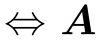
\includegraphics[width=28.81pt]{images-full/p017-i000.png}}\allowbreak{} 的特征值均不为0
\allowbreak{}\raisebox{-2.28pt}{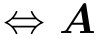
\includegraphics[width=28.25pt]{images-full/p017-i001.png}}\allowbreak{} 的伴随矩阵\allowbreak{}\raisebox{-2.40pt}{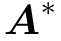
\includegraphics[width=16.95pt]{images-full/p017-i002.png}}\allowbreak{} 可逆
\allowbreak{}\raisebox{-2.28pt}{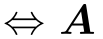
\includegraphics[width=28.81pt]{images-full/p017-i003.png}}\allowbreak{} 是一些初等矩阵之积.
\par\medskip\noindent\textbf{【例1.2.6 】设\allowbreak{}\raisebox{-2.76pt}{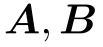
\includegraphics[width=28.81pt]{images-full/p017-i004.png}}\allowbreak{} 均为$n$ 阶方阵若\allowbreak{}\raisebox{-2.28pt}{
\includegraphics[width=47.77pt]{images-full/p017-i006.png}}\allowbreak{} 可逆，证明\allowbreak{}\raisebox{-2.28pt}{
\includegraphics[width=47.93pt]{images-full/p017-i007.png}}\allowbreak{} 可逆，并求}
\sourceblock{355.38}{images-full/p017-d000.png}
因此
\sourceblock{192.66}{images-full/p017-d001.png}
由于\allowbreak{}\raisebox{-2.28pt}{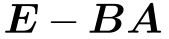
\includegraphics[width=47.46pt]{images-full/p017-i008.png}}\allowbreak{} 可逆，即\allowbreak{}\raisebox{-3.00pt}{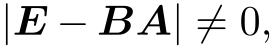
\includegraphics[width=77.97pt]{images-full/p017-i009.png}}\allowbreak{}，所以\allowbreak{}\raisebox{-3.00pt}{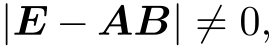
\includegraphics[width=75.78pt]{images-full/p017-i010.png}}\allowbreak{}，因此\allowbreak{}\raisebox{-2.28pt}{
\includegraphics[width=47.36pt]{images-full/p017-i011.png}}\allowbreak{} 可逆. 下
面进一步求\allowbreak{}\raisebox{-3.24pt}{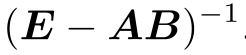
\includegraphics[width=69.39pt]{images-full/p017-i012.png}}\allowbreak{} 由于
\sourceblock{185.88}{images-full/p017-d002.png}
故
\sourceblock{228.26}{images-full/p017-d003.png}
进而
\sourceblock{201.14}{images-full/p017-d004.png}
\sourceblock{326.57}{images-full/p019-d002.png}
\sourceblock{276.85}{images-full/p019-d003.png}
\par\noindent (3) 定义法，由\allowbreak{}\raisebox{-2.28pt}{
\includegraphics[width=50.85pt]{images-full/p019-i004.png}}\allowbreak{} 求出\allowbreak{}\raisebox{-2.28pt}{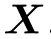
\includegraphics[width=14.16pt]{images-full/p019-i005.png}}\allowbreak{}
若矩阵$A$ 没有具体给出，是抽象的，则首先想到的是用定义来求\allowbreak{}\raisebox{-2.76pt}{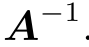
\includegraphics[width=24.62pt]{images-full/p019-i007.png}}\allowbreak{}.
\sourceblock{300.01}{images-full/p022-d004.png}
矩阵的行列式是矩阵的一个数值特征.矩阵的数值特征还有矩阵的秩、矩阵的特征
\sourceblock{357.64}{images-full/p022-d005.png}
\sourceblock{132.21}{images-full/p022-d006.png}
计算\allowbreak{}\raisebox{-3.00pt}{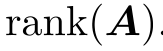
\includegraphics[width=45.83pt]{images-full/p022-i000.png}}\allowbreak{}


% SOURCE_PDF_PAGE 23

\hypertarget{source-p023}{}
\par\noindent\textbf{解}\ 
\sourceblock{389.85}{images-full/p023-d000.png}
\sourceblock{450.00}{images-full/p023-d001.png}
\par\medskip\noindent\textbf{【例1.2.13 】设$A$ 为2023 阶非军实矩阵. \allowbreak{}\raisebox{-3.00pt}{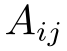
\includegraphics[width=18.64pt]{images-full/p023-i001.png}}\allowbreak{} 为$A$ 中元素\allowbreak{}\raisebox{-2.28pt}{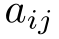
\includegraphics[width=16.38pt]{images-full/p023-i003.png}}\allowbreak{}的代数余子式且}
\allowbreak{}\raisebox{-3.00pt}{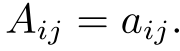
\includegraphics[width=50.51pt]{images-full/p023-i004.png}}\allowbreak{}·求$A$ 的秩与行列式.
解由于\allowbreak{}\raisebox{-2.76pt}{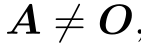
\includegraphics[width=39.55pt]{images-full/p023-i006.png}}\allowbreak{}，不妨设\allowbreak{}\raisebox{-2.76pt}{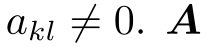
\includegraphics[width=58.17pt]{images-full/p023-i007.png}}\allowbreak{} 按第$k$ 行展开有
\sourceblock{166.67}{images-full/p023-d002.png}
故\allowbreak{}\raisebox{-3.00pt}{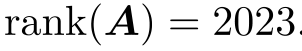
\includegraphics[width=84.87pt]{images-full/p023-i009.png}}\allowbreak{}.
由己知布$A$ 的伴随矩阵\allowbreak{}\raisebox{-2.76pt}{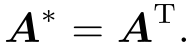
\includegraphics[width=52.75pt]{images-full/p023-i011.png}}\allowbreak{}所以由\allowbreak{}\raisebox{-3.00pt}{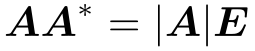
\includegraphics[width=71.75pt]{images-full/p023-i012.png}}\allowbreak{} 有\allowbreak{}\raisebox{-3.36pt}{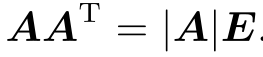
\includegraphics[width=74.22pt]{images-full/p023-i013.png}}\allowbreak{}. 两边取
行列式有
\sourceblock{328.26}{images-full/p023-d003.png}
\sourceblock{416.97}{images-full/p024-d001.png}
解根据rank(A) 的情况讨论
\sourceblock{450.00}{images-full/p024-d002.png}
\sourceblock{450.00}{images-full/p024-d003.png}
\sourceblock{344.65}{images-full/p024-d004.png}


% SOURCE_PDF_PAGE 25

\hypertarget{source-p025}{}
设矩阵$A$ 的特征值为\allowbreak{}\raisebox{-2.76pt}{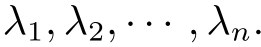
\includegraphics[width=73.36pt]{images-full/p025-i001.png}}\allowbreak{} 求矩阵$B$ 的特征值.
解矩阵$A$ 和$B$ 的特征多项式分别为
\sourceblock{272.33}{images-full/p025-d000.png}
\sourceblock{311.88}{images-full/p025-d001.png}
当$n=l$ 时，
\sourceblock{140.12}{images-full/p025-d002.png}
当\allowbreak{}\raisebox{-2.28pt}{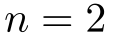
\includegraphics[width=31.64pt]{images-full/p025-i006.png}}\allowbreak{} 时，
\sourceblock{287.02}{images-full/p025-d003.png}
\sourceblock{107.35}{images-full/p025-d004.png}
设\allowbreak{}\raisebox{-2.64pt}{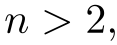
\includegraphics[width=32.85pt]{images-full/p025-i007.png}}\allowbreak{}则有
\sourceblock{256.51}{images-full/p025-d005.png}
\sourceblock{450.00}{images-full/p025-d006.png}
\par\medskip\noindent\textbf{【例1.2.17】设1013 阶实方阵$A$ 可对角化且满足}
\sourceblock{141.25}{images-full/p025-d007.png}


% SOURCE_PDF_PAGE 26

\hypertarget{source-p026}{}
和
\sourceblock{101.13}{images-full/p026-d000.png}
求$A$ 的特征值.
解由于$A$ 可对角化，故$A$ 的每个特征值的代数重数等于其几何重数.令\allowbreak{}\raisebox{-2.28pt}{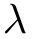
\includegraphics[width=9.04pt]{images-full/p026-i003.png}}\allowbreak{} 为$A$
的特征值，则有
\sourceblock{122.04}{images-full/p026-d001.png}
即
\sourceblock{117.52}{images-full/p026-d002.png}
\sourceblock{107.35}{images-full/p026-d003.png}
故$A$ 的特征值只可能是\allowbreak{}\raisebox{-2.64pt}{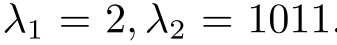
\includegraphics[width=94.83pt]{images-full/p026-i006.png}}\allowbreak{}.注意到\allowbreak{}\raisebox{-3.00pt}{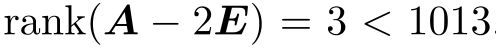
\includegraphics[width=139.88pt]{images-full/p026-i007.png}}\allowbreak{} 所以2
是$A$ 的一个特征值.
由于可对角化，特征值2 的代数重数等于其几何重数.由于\allowbreak{}\raisebox{-3.00pt}{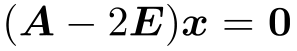
\includegraphics[width=83.62pt]{images-full/p026-i009.png}}\allowbreak{} 的解空
间维数为\allowbreak{}\raisebox{-3.00pt}{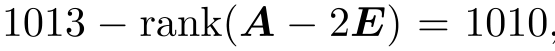
\includegraphics[width=156.52pt]{images-full/p026-i010.png}}\allowbreak{}，因此2 作为$A$ 的特征值，其代数重数为1010.
故$A$ 还有其他特征值，且一定为1011. 其代数重数为\allowbreak{}\raisebox{-2.16pt}{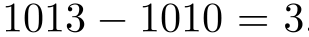
\includegraphics[width=86.91pt]{images-full/p026-i013.png}}\allowbreak{} 至此$A$ 的全部
特征值为\allowbreak{}\raisebox{-3.00pt}{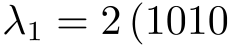
\includegraphics[width=66.10pt]{images-full/p026-i015.png}}\allowbreak{} 重)，\allowbreak{}\raisebox{-3.00pt}{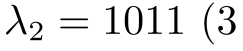
\includegraphics[width=68.36pt]{images-full/p026-i016.png}}\allowbreak{} 重) .
【注1.2.31前面例1.2.16 和例1.2.17 考察的是抽象矩阵特征值的计算问题.
\par\medskip\noindent\textbf{【例1.2.18 】设$A$ 为3 阶实对称矩阵，\allowbreak{}\raisebox{-3.00pt}{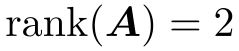
\includegraphics[width=67.23pt]{images-full/p026-i018.png}}\allowbreak{} 且}
\sourceblock{285.32}{images-full/p026-d004.png}
\par\noindent (2) 矩阵$A$
\sourceblock{450.00}{images-full/p026-d005.png}
属于特征值。的特征向量，则有


% SOURCE_PDF_PAGE 27

\hypertarget{source-p027}{}
\sourceblock{79.10}{images-full/p027-d000.png}
\sourceblock{346.91}{images-full/p027-d001.png}
\sourceblock{375.16}{images-full/p027-d002.png}
\sourceblock{410.19}{images-full/p027-d003.png}
的全部特征值.
解(方法1) 首先计算\allowbreak{}\raisebox{-2.88pt}{
\includegraphics[width=18.08pt]{images-full/p027-i000.png}}\allowbreak{} 以便确定。是否为$A$ 的特征值.易知


% SOURCE_PDF_PAGE 28

\hypertarget{source-p028}{}
\sourceblock{240.12}{images-full/p028-d000.png}
故\allowbreak{}\raisebox{-2.28pt}{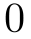
\includegraphics[width=8.47pt]{images-full/p028-i000.png}}\allowbreak{} 是$A$ 的特征值.下面确定\allowbreak{}\raisebox{-2.28pt}{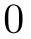
\includegraphics[width=8.47pt]{images-full/p028-i002.png}}\allowbreak{} 的代数重数.
由于\allowbreak{}\raisebox{-3.00pt}{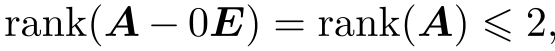
\includegraphics[width=156.43pt]{images-full/p028-i003.png}}\allowbreak{}，因此\allowbreak{}\raisebox{-2.28pt}{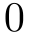
\includegraphics[width=8.47pt]{images-full/p028-i004.png}}\allowbreak{} 的代数重数\allowbreak{}\raisebox{-2.52pt}{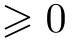
\includegraphics[width=20.34pt]{images-full/p028-i005.png}}\allowbreak{} 的儿何重数\allowbreak{}\raisebox{-2.64pt}{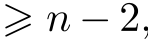
\includegraphics[width=41.44pt]{images-full/p028-i006.png}}\allowbreak{}，即
$A$ 至少有\allowbreak{}\raisebox{-2.16pt}{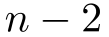
\includegraphics[width=30.51pt]{images-full/p028-i008.png}}\allowbreak{} 个特征值为\allowbreak{}\raisebox{-2.16pt}{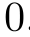
\includegraphics[width=8.12pt]{images-full/p028-i009.png}}\allowbreak{}
\sourceblock{205.09}{images-full/p028-d001.png}
\sourceblock{390.98}{images-full/p028-d002.png}
故\allowbreak{}\raisebox{-2.28pt}{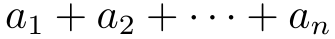
\includegraphics[width=94.35pt]{images-full/p028-i010.png}}\allowbreak{}也是$A$ 的特征值，而
\sourceblock{226.56}{images-full/p028-d003.png}
故\allowbreak{}\raisebox{-2.64pt}{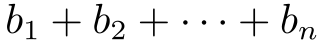
\includegraphics[width=90.96pt]{images-full/p028-i012.png}}\allowbreak{} 是\allowbreak{}\raisebox{-2.76pt}{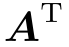
\includegraphics[width=19.21pt]{images-full/p028-i013.png}}\allowbreak{} 的特征值.从丽也是$A$ 的特征值.
\sourceblock{372.33}{images-full/p028-d004.png}
若\allowbreak{}\raisebox{-2.88pt}{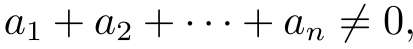
\includegraphics[width=116.29pt]{images-full/p028-i015.png}}\allowbreak{}，则\allowbreak{}\raisebox{-2.40pt}{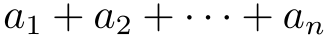
\includegraphics[width=93.22pt]{images-full/p028-i016.png}}\allowbreak{}为$A$ 的一个非零特征值，从而\allowbreak{}\raisebox{-2.64pt}{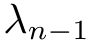
\includegraphics[width=25.99pt]{images-full/p028-i018.png}}\allowbreak{}
\sourceblock{450.00}{images-full/p028-d005.png}
最后考察\allowbreak{}\raisebox{-2.64pt}{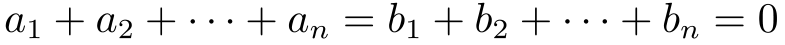
\includegraphics[width=221.48pt]{images-full/p028-i019.png}}\allowbreak{} 的情形.
注意到$A$ 的特征多项式\allowbreak{}\raisebox{-2.76pt}{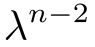
\includegraphics[width=26.55pt]{images-full/p028-i021.png}}\allowbreak{} 的系数是$A$ 的所有三阶主子式之和. 从而
\sourceblock{194.92}{images-full/p028-d006.png}


% SOURCE_PDF_PAGE 29

\hypertarget{source-p029}{}
\sourceblock{236.17}{images-full/p029-d000.png}
\sourceblock{351.99}{images-full/p029-d001.png}
因此\allowbreak{}\raisebox{-2.76pt}{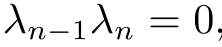
\includegraphics[width=62.41pt]{images-full/p029-i000.png}}\allowbreak{}，又\allowbreak{}\raisebox{-2.76pt}{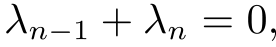
\includegraphics[width=77.76pt]{images-full/p029-i001.png}}\allowbreak{}，从而\allowbreak{}\raisebox{-2.64pt}{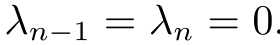
\includegraphics[width=78.78pt]{images-full/p029-i002.png}}\allowbreak{} 这时$A$ 的全部特征值均
为\allowbreak{}\raisebox{-3.00pt}{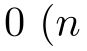
\includegraphics[width=24.29pt]{images-full/p029-i004.png}}\allowbreak{} 重).
(方法2) 根据题设可知，矩阵$A$ 可表示为
\sourceblock{241.82}{images-full/p029-d002.png}
其中
\sourceblock{248.03}{images-full/p029-d003.png}
利用行列式降阶公式，矩阵$A$ 的特征多项式可化为
\sourceblock{232.21}{images-full/p029-d004.png}
\sourceblock{274.02}{images-full/p029-d005.png}


% SOURCE_PDF_PAGE 30

\hypertarget{source-p030}{}
\sourceblock{367.81}{images-full/p030-d000.png}
\sourceblock{416.40}{images-full/p030-d001.png}
\sourceblock{330.52}{images-full/p030-d002.png}
\sourceblock{157.63}{images-full/p030-d003.png}
\sourceblock{106.78}{images-full/p030-d004.png}
\sourceblock{92.09}{images-full/p030-d005.png}
以及tr(A) 为A 的n 个特征值的和.
\sourceblock{248.03}{images-full/p030-d006.png}
解容易计算
\sourceblock{233.34}{images-full/p030-d007.png}
利用数学归纳法容易证明
\sourceblock{238.99}{images-full/p030-d008.png}
从而
\sourceblock{177.97}{images-full/p030-d009.png}


% SOURCE_PDF_PAGE 31

\hypertarget{source-p031}{}
\sourceblock{450.00}{images-full/p031-d000.png}
\sourceblock{450.00}{images-full/p031-d001.png}
矩阵，所以\allowbreak{}\raisebox{-2.52pt}{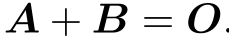
\includegraphics[width=64.40pt]{images-full/p031-i000.png}}\allowbreak{}
\sourceblock{433.35}{images-full/p031-d002.png}
$A$ 为对称矩阵
\par\noindent\textbf{证明}\ 由于
\sourceblock{163.85}{images-full/p031-d003.png}
所以
\sourceblock{355.38}{images-full/p031-d004.png}
即$A$ 为对称矩阵.口


% SOURCE_PDF_PAGE 32

\hypertarget{source-p032}{}
园也型A据眸圳特征份估针咱也
线性代数中常考虑、关于矩阵特征值、秩、迹等数值特征的估计问题.这类问题多以不
等式形式出现.解决此类问题时大多需利用相关的性质.有时还需要较强的技巧.
\sourceblock{450.00}{images-full/p032-d007.png}


% SOURCE_PDF_PAGE 33

\hypertarget{source-p033}{}
\par\noindent\textbf{证明}\ 若\allowbreak{}\raisebox{-2.76pt}{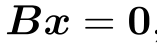
\includegraphics[width=44.21pt]{images-full/p033-i000.png}}\allowbreak{}，则\allowbreak{}\raisebox{-2.76pt}{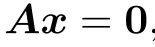
\includegraphics[width=43.37pt]{images-full/p033-i001.png}}\allowbreak{}，因而\allowbreak{}\raisebox{-3.00pt}{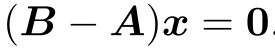
\includegraphics[width=77.37pt]{images-full/p033-i002.png}}\allowbreak{} 故\allowbreak{}\raisebox{-3.00pt}{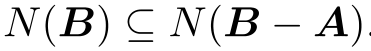
\includegraphics[width=104.59pt]{images-full/p033-i003.png}}\allowbreak{} 因此
\sourceblock{287.58}{images-full/p033-d000.png}
从而
\sourceblock{289.84}{images-full/p033-d001.png}
\sourceblock{401.15}{images-full/p033-d002.png}
\sourceblock{450.00}{images-full/p033-d003.png}
取$B$ 为单位矩阵，即得Sylvester 不等式.
\par\medskip\noindent\textbf{【例1.2.25 】设\allowbreak{}\raisebox{-2.76pt}{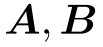
\includegraphics[width=28.81pt]{images-full/p033-i005.png}}\allowbreak{} 为$n$ 阶矩阵，\allowbreak{}\raisebox{-2.40pt}{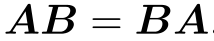
\includegraphics[width=60.29pt]{images-full/p033-i007.png}}\allowbreak{} 证明}
\sourceblock{259.33}{images-full/p033-d004.png}
\par\noindent\textbf{证明}\ 由\allowbreak{}\raisebox{-2.40pt}{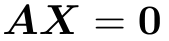
\includegraphics[width=47.46pt]{images-full/p033-i008.png}}\allowbreak{} 和\allowbreak{}\raisebox{-2.28pt}{
\includegraphics[width=48.02pt]{images-full/p033-i009.png}}\allowbreak{} 有\allowbreak{}\raisebox{-3.00pt}{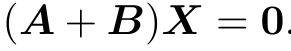
\includegraphics[width=81.84pt]{images-full/p033-i010.png}}\allowbreak{} 从而
\sourceblock{150.85}{images-full/p033-d005.png}
显然
\sourceblock{407.93}{images-full/p033-d006.png}
\sourceblock{370.07}{images-full/p033-d007.png}
故\allowbreak{}\raisebox{-3.00pt}{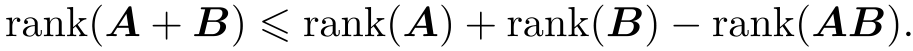
\includegraphics[width=257.70pt]{images-full/p033-i011.png}}\allowbreak{} 口


% SOURCE_PDF_PAGE 34

\hypertarget{source-p034}{}
\sourceblock{450.00}{images-full/p034-d000.png}
\sourceblock{332.22}{images-full/p034-d001.png}
可得
\sourceblock{296.06}{images-full/p034-d002.png}
\par\medskip\noindent\textbf{【例1.2.27】设$A$ 为$n$ 阶反对称实矩阵.证明关于$X$ 的矩阵方程\allowbreak{}\raisebox{-2.40pt}{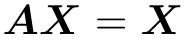
\includegraphics[width=53.11pt]{images-full/p034-i003.png}}\allowbreak{} 只}
有零解.
\par\noindent\textbf{证明}\ 由\allowbreak{}\raisebox{-2.28pt}{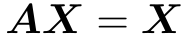
\includegraphics[width=52.54pt]{images-full/p034-i004.png}}\allowbreak{} 得\allowbreak{}\raisebox{-3.24pt}{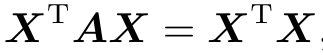
\includegraphics[width=90.88pt]{images-full/p034-i005.png}}\allowbreak{}，于是
\sourceblock{312.44}{images-full/p034-d003.png}
从而\allowbreak{}\raisebox{-3.48pt}{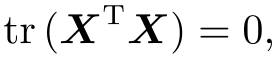
\includegraphics[width=78.43pt]{images-full/p034-i006.png}}\allowbreak{}，所以\allowbreak{}\raisebox{-2.28pt}{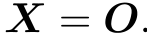
\includegraphics[width=41.22pt]{images-full/p034-i007.png}}\allowbreak{}口
\sourceblock{372.33}{images-full/p034-d004.png}
\par\noindent\textbf{证明}\ 令\allowbreak{}\raisebox{-3.00pt}{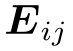
\includegraphics[width=20.34pt]{images-full/p034-i008.png}}\allowbreak{}表示\allowbreak{}\raisebox{-3.00pt}{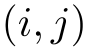
\includegraphics[width=25.42pt]{images-full/p034-i009.png}}\allowbreak{} 元素为1，其他元素均为\allowbreak{}\raisebox{-2.28pt}{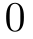
\includegraphics[width=9.04pt]{images-full/p034-i010.png}}\allowbreak{} 的$n$ 阶方阵，则
\sourceblock{396.06}{images-full/p034-d005.png}
注意到
\sourceblock{114.69}{images-full/p034-d006.png}
\sourceblock{341.82}{images-full/p034-d007.png}
\sourceblock{143.51}{images-full/p034-d008.png}
另一方面，若\allowbreak{}\raisebox{-2.88pt}{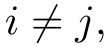
\includegraphics[width=29.31pt]{images-full/p034-i012.png}}\allowbreak{}则\allowbreak{}\raisebox{-2.88pt}{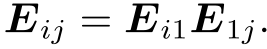
\includegraphics[width=75.01pt]{images-full/p034-i013.png}}\allowbreak{} 从而


% SOURCE_PDF_PAGE 35

\hypertarget{source-p035}{}
\sourceblock{370.07}{images-full/p035-d000.png}
所以，对任意\allowbreak{}\raisebox{-3.12pt}{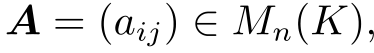
\includegraphics[width=105.32pt]{images-full/p035-i000.png}}\allowbreak{}，有
\sourceblock{362.16}{images-full/p035-d001.png}
\par\medskip\noindent\textbf{【例1.2.29 】设$A$ 为$n$ 阶实矩阵，且$E-A$ 的特征值的模均小于1.证明\allowbreak{}\raisebox{-2.28pt}{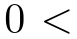
\includegraphics[width=21.47pt]{images-full/p035-i004.png}}\allowbreak{}}
\sourceblock{49.15}{images-full/p035-d002.png}
\par\noindent\textbf{证明}\ 设$A$ 的复特征值为机\allowbreak{}\raisebox{-2.76pt}{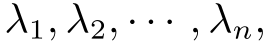
\includegraphics[width=73.97pt]{images-full/p035-i006.png}}\allowbreak{}，则$E-A$ 的特征值为\allowbreak{}\raisebox{-2.76pt}{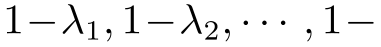
\includegraphics[width=107.35pt]{images-full/p035-i008.png}}\allowbreak{}
\allowbreak{}\raisebox{-2.64pt}{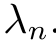
\includegraphics[width=15.44pt]{images-full/p035-i009.png}}\allowbreak{}.故对任意$i$，
\sourceblock{63.84}{images-full/p035-d003.png}
若\allowbreak{}\raisebox{-2.76pt}{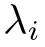
\includegraphics[width=12.43pt]{images-full/p035-i011.png}}\allowbreak{} 为实数，由\allowbreak{}\raisebox{-2.88pt}{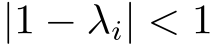
\includegraphics[width=61.02pt]{images-full/p035-i012.png}}\allowbreak{} 得\allowbreak{}\raisebox{-2.76pt}{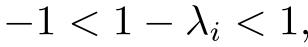
\includegraphics[width=86.65pt]{images-full/p035-i013.png}}\allowbreak{}，即\allowbreak{}\raisebox{-2.76pt}{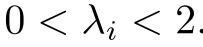
\includegraphics[width=57.11pt]{images-full/p035-i014.png}}\allowbreak{}.
若\allowbreak{}\raisebox{-2.64pt}{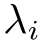
\includegraphics[width=12.43pt]{images-full/p035-i015.png}}\allowbreak{}为非实数，则\allowbreak{}\raisebox{-3.12pt}{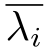
\includegraphics[width=14.12pt]{images-full/p035-i016.png}}\allowbreak{}也是$A$ 的特征值.此时
\sourceblock{200.57}{images-full/p035-d004.png}
这时
\sourceblock{91.53}{images-full/p035-d005.png}
由\allowbreak{}\raisebox{-3.00pt}{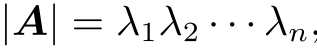
\includegraphics[width=89.12pt]{images-full/p035-i018.png}}\allowbreak{}可得\allowbreak{}\raisebox{-3.00pt}{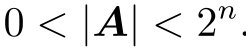
\includegraphics[width=69.07pt]{images-full/p035-i019.png}}\allowbreak{} 口
\par\medskip\noindent\textbf{【例1.2.30 】设\allowbreak{}\raisebox{-2.76pt}{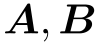
\includegraphics[width=28.81pt]{images-full/p035-i020.png}}\allowbreak{} 分别为$m$ 阶和$n$ 阶方阵，$C$ 为\allowbreak{}\raisebox{-1.80pt}{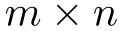
\includegraphics[width=34.46pt]{images-full/p035-i024.png}}\allowbreak{} 矩阵，且满足}
\sourceblock{144.64}{images-full/p035-d006.png}
\par\noindent\textbf{证明}\ $A$ 与$B$ 至少有\allowbreak{}\raisebox{-1.68pt}{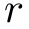
\includegraphics[width=7.91pt]{images-full/p035-i027.png}}\allowbreak{}个相同的特征值(包括重数).
\par\noindent\textbf{证明}\ 由于\allowbreak{}\raisebox{-3.00pt}{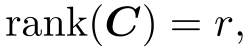
\includegraphics[width=68.62pt]{images-full/p035-i028.png}}\allowbreak{}故存在$m$ 阶可逆矩阵\allowbreak{}\raisebox{-2.76pt}{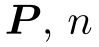
\includegraphics[width=27.68pt]{images-full/p035-i030.png}}\allowbreak{} 阶可逆矩阵$Q$，使得
\sourceblock{120.91}{images-full/p035-d007.png}
由\allowbreak{}\raisebox{-2.28pt}{
\includegraphics[width=60.45pt]{images-full/p035-i032.png}}\allowbreak{} 得到
\sourceblock{277.41}{images-full/p035-d008.png}
即
\sourceblock{358.21}{images-full/p035-d009.png}


% SOURCE_PDF_PAGE 36

\hypertarget{source-p036}{}
\sourceblock{245.77}{images-full/p036-d000.png}
令
\sourceblock{435.05}{images-full/p036-d001.png}
\sourceblock{389.85}{images-full/p036-d002.png}
这里用到\allowbreak{}\raisebox{-2.64pt}{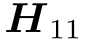
\includegraphics[width=23.73pt]{images-full/p036-i000.png}}\allowbreak{}有$T$ 个特征值，这对任意数域不一定成立.但显然复数域上的矩阵
\allowbreak{}\raisebox{-2.64pt}{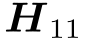
\includegraphics[width=23.73pt]{images-full/p036-i002.png}}\allowbreak{} 的$T$个特征值是$H$ 与$T$ 的公共特征值.注意到$A$ 与$H$ 相似，$B$ 与$T$ 相似.故
$A$ 与$H$ 有相同的特征值，$B$ 与$T$ 有相同的特征值.因此$A$ 与$B$ 至少有$T$个相同的特
征值.口
园也型λ悦和等支挤在帕
此类型题目通常考察下面内容:
\par\noindent (1) 利用分块初等变换进行降阶计算.
\par\noindent (2) 初等矩阵与初等变换的关系.
\par\noindent (3) 分块矩阵的性质及其计算.
解题中熟记下列基本结果是有帮助的:
\sourceblock{210.74}{images-full/p036-d003.png}


% SOURCE_PDF_PAGE 37

\hypertarget{source-p037}{}
\sourceblock{210.18}{images-full/p037-d000.png}
\sourceblock{394.37}{images-full/p037-d001.png}
所以
\sourceblock{300.01}{images-full/p037-d002.png}
故
\sourceblock{409.62}{images-full/p037-d003.png}
由
\sourceblock{344.65}{images-full/p037-d004.png}
\sourceblock{378.55}{images-full/p037-d005.png}
\sourceblock{304.53}{images-full/p037-d006.png}
\sourceblock{450.00}{images-full/p037-d007.png}
\par\noindent\textbf{证明}\ 对矩阵$Q$ 施行分块初等变换
\sourceblock{206.79}{images-full/p037-d008.png}
\sourceblock{380.24}{images-full/p037-d009.png}


% SOURCE_PDF_PAGE 38

\hypertarget{source-p038}{}
于是\allowbreak{}\raisebox{-3.36pt}{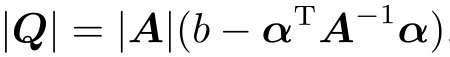
\includegraphics[width=127.04pt]{images-full/p038-i000.png}}\allowbreak{}，由于\allowbreak{}\raisebox{-3.00pt}{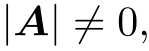
\includegraphics[width=42.01pt]{images-full/p038-i001.png}}\allowbreak{}，故
\sourceblock{293.80}{images-full/p038-d000.png}
\par\medskip\noindent\textbf{【例1.2.32 】设$A$ 为$m$ 阶可逆矩阵，$B$ 为\allowbreak{}\raisebox{-1.80pt}{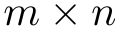
\includegraphics[width=34.46pt]{images-full/p038-i005.png}}\allowbreak{} 矩阵，$C$ 为\allowbreak{}\raisebox{-1.80pt}{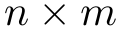
\includegraphics[width=34.46pt]{images-full/p038-i007.png}}\allowbreak{} 矩阵，$D$ 为}
$n$阶方阵.证明
\sourceblock{174.58}{images-full/p038-d001.png}
\par\noindent\textbf{证明}\ 困
\sourceblock{381.94}{images-full/p038-d002.png}
进一步地，若\allowbreak{}\raisebox{-2.76pt}{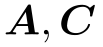
\includegraphics[width=28.81pt]{images-full/p038-i010.png}}\allowbreak{} 可交换，则
\sourceblock{353.12}{images-full/p038-d003.png}
【注1.2.7】此例中，若$D$ 也可逆，则杳
\sourceblock{207.35}{images-full/p038-d004.png}
从而
\sourceblock{166.67}{images-full/p038-d005.png}
由此得到
\sourceblock{207.92}{images-full/p038-d006.png}
以\allowbreak{}\raisebox{-2.28pt}{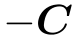
\includegraphics[width=22.03pt]{images-full/p038-i012.png}}\allowbreak{}代替上式中的$C$ 可得
\sourceblock{207.92}{images-full/p038-d007.png}
这个等式也称为行列式的降阶公式.
特别地，若取\allowbreak{}\raisebox{-2.76pt}{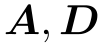
\includegraphics[width=29.38pt]{images-full/p038-i014.png}}\allowbreak{} 为单位矩阵，则有\allowbreak{}\raisebox{-3.00pt}{
\includegraphics[width=138.14pt]{images-full/p038-i015.png}}\allowbreak{}


% SOURCE_PDF_PAGE 39

\hypertarget{source-p039}{}
\par\medskip\noindent\textbf{【例1.2.33 】设\allowbreak{}\raisebox{-2.76pt}{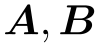
\includegraphics[width=28.81pt]{images-full/p039-i000.png}}\allowbreak{} 为$n$ 阶矩阵证明}
\sourceblock{250.29}{images-full/p039-d000.png}
\sourceblock{405.10}{images-full/p039-d001.png}
所以
\sourceblock{436.18}{images-full/p039-d002.png}
(方法2) 直接利用关于矩阵秩的不等式，得
\sourceblock{362.73}{images-full/p039-d003.png}
\par\medskip\noindent\textbf{【例1.2.34】令}
\sourceblock{243.51}{images-full/p039-d004.png}
求\allowbreak{}\raisebox{-3.00pt}{
\includegraphics[width=18.15pt]{images-full/p039-i002.png}}\allowbreak{}
解易知
\sourceblock{249.73}{images-full/p039-d005.png}
\sourceblock{317.53}{images-full/p039-d006.png}


% SOURCE_PDF_PAGE 40

\hypertarget{source-p040}{}
\sourceblock{267.24}{images-full/p040-d000.png}
\par\medskip\noindent\textbf{【例1.2.36 】设\allowbreak{}\raisebox{-2.76pt}{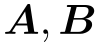
\includegraphics[width=28.81pt]{images-full/p041-i000.png}}\allowbreak{} 均为\allowbreak{}\raisebox{-1.68pt}{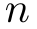
\includegraphics[width=10.17pt]{images-full/p041-i001.png}}\allowbreak{} 阶实矩阵，证明}
\sourceblock{202.83}{images-full/p041-d001.png}
\par\noindent\textbf{证明}\ 困为
\sourceblock{406.23}{images-full/p041-d002.png}
\sourceblock{181.36}{images-full/p041-d003.png}
进一步地，
\sourceblock{329.96}{images-full/p041-d004.png}
\sourceblock{108.48}{images-full/p041-d005.png}
\sourceblock{262.16}{images-full/p041-d006.png}


% SOURCE_PDF_PAGE 42

\hypertarget{source-p042}{}
解注意到
\sourceblock{262.72}{images-full/p042-d000.png}
\sourceblock{450.00}{images-full/p042-d001.png}
\sourceblock{392.67}{images-full/p042-d002.png}
\par\noindent (2) 求满足\allowbreak{}\raisebox{-2.28pt}{
\includegraphics[width=51.41pt]{images-full/p042-i000.png}}\allowbreak{} 的所杳三阶矩阵\allowbreak{}\raisebox{-2.28pt}{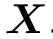
\includegraphics[width=14.63pt]{images-full/p042-i001.png}}\allowbreak{}


% SOURCE_PDF_PAGE 43

\hypertarget{source-p043}{}
\sourceblock{374.59}{images-full/p043-d000.png}
\sourceblock{385.33}{images-full/p043-d001.png}
\sourceblock{290.97}{images-full/p043-d002.png}
\sourceblock{322.05}{images-full/p043-d003.png}


% SOURCE_PDF_PAGE 44

\hypertarget{source-p044}{}
从而
\sourceblock{450.00}{images-full/p044-d000.png}
\sourceblock{445.22}{images-full/p044-d001.png}
对右边直接计算得
\sourceblock{282.50}{images-full/p044-d002.png}
所以
\sourceblock{339.56}{images-full/p044-d003.png}


% SOURCE_PDF_PAGE 45

\hypertarget{source-p045}{}
园也型々t.'tiJð-创刊的制确定
\par\medskip\noindent\textbf{【例1.2.41 】设$B$ 为$p$ 阶复方阵，}
\sourceblock{184.19}{images-full/p046-d000.png}
试求$B$ 的初等因子.
解显然，$B$ 的特征多项式为\allowbreak{}\raisebox{-3.00pt}{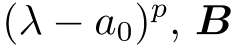
\includegraphics[width=66.53pt]{images-full/p046-i004.png}}\allowbreak{} 的特征值都等于\allowbreak{}\raisebox{-2.04pt}{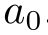
\includegraphics[width=13.52pt]{images-full/p046-i005.png}}\allowbreak{}.
\par\noindent (1) 当\allowbreak{}\raisebox{-2.76pt}{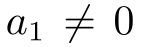
\includegraphics[width=39.55pt]{images-full/p046-i006.png}}\allowbreak{} 时，\allowbreak{}\raisebox{-3.00pt}{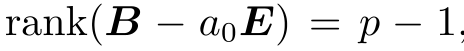
\includegraphics[width=130.73pt]{images-full/p046-i007.png}}\allowbreak{}，特征值\allowbreak{}\raisebox{-2.04pt}{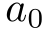
\includegraphics[width=13.56pt]{images-full/p046-i008.png}}\allowbreak{} 的儿何重数为1.故$B$ 的
Jordan 标准形中只能有一个Jordan 块，即$B$ 只有一个初等因子\allowbreak{}\raisebox{-3.00pt}{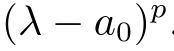
\includegraphics[width=48.79pt]{images-full/p046-i011.png}}\allowbreak{}.
\par\noindent (2) 当\allowbreak{}\raisebox{-2.88pt}{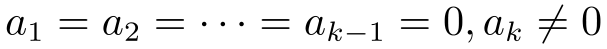
\includegraphics[width=171.19pt]{images-full/p046-i012.png}}\allowbreak{} 时，为找出$B$ 的所有初等因子，我们先来确
定$B$ 的Jordan 标准形中Jordan 块的形状和个数.
注意到
\sourceblock{362.73}{images-full/p046-d001.png}
\par \allowbreak{}\raisebox{-3.48pt}{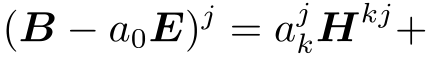
\includegraphics[width=121.47pt]{images-full/p046-i015.png}}\allowbreak{}若干$H$ 的更高罪次项.
所以
\sourceblock{331.65}{images-full/p046-d002.png}
记\allowbreak{}\raisebox{-3.00pt}{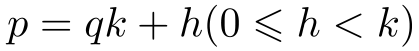
\includegraphics[width=118.08pt]{images-full/p046-i017.png}}\allowbreak{}(带余除法) ，则
\sourceblock{269.50}{images-full/p046-d003.png}
现假设$B$ 的初等因子有\allowbreak{}\raisebox{-2.16pt}{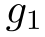
\includegraphics[width=12.43pt]{images-full/p046-i019.png}}\allowbreak{}个\allowbreak{}\raisebox{-2.88pt}{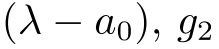
\includegraphics[width=61.58pt]{images-full/p046-i020.png}}\allowbreak{} 个\allowbreak{}\raisebox{-3.36pt}{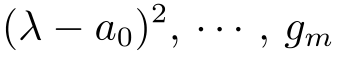
\includegraphics[width=95.48pt]{images-full/p046-i021.png}}\allowbreak{} 个\allowbreak{}\raisebox{-3.00pt}{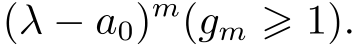
\includegraphics[width=99.82pt]{images-full/p046-i022.png}}\allowbreak{}
对此$B$ 有相应的Jordan 标准形.从$B$ 的这个Jordan 标准形又可定义出各个\allowbreak{}\raisebox{-3.00pt}{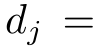
\includegraphics[width=27.68pt]{images-full/p046-i025.png}}\allowbreak{}


% SOURCE_PDF_PAGE 47

\hypertarget{source-p047}{}
\allowbreak{}\raisebox{-3.24pt}{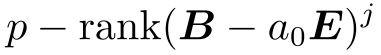
\includegraphics[width=107.35pt]{images-full/p047-i000.png}}\allowbreak{} 的值:
\sourceblock{190.97}{images-full/p047-d000.png}
将这组\allowbreak{}\raisebox{-3.00pt}{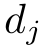
\includegraphics[width=12.99pt]{images-full/p047-i001.png}}\allowbreak{}的值与前面己经得到的值进行比较，可得
\sourceblock{214.13}{images-full/p047-d001.png}
\sourceblock{303.40}{images-full/p047-d002.png}
所以当\allowbreak{}\raisebox{-2.88pt}{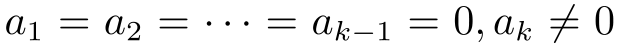
\includegraphics[width=175.15pt]{images-full/p047-i002.png}}\allowbreak{} 时$B$ 的初等因子有:$k-h$ 个\allowbreak{}\raisebox{-3.00pt}{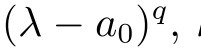
\includegraphics[width=56.54pt]{images-full/p047-i005.png}}\allowbreak{}h 个
\allowbreak{}\raisebox{-3.24pt}{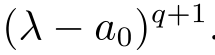
\includegraphics[width=60.51pt]{images-full/p047-i006.png}}\allowbreak{}
\par\noindent (3) 最后，显然当\allowbreak{}\raisebox{-2.88pt}{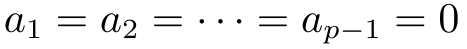
\includegraphics[width=131.64pt]{images-full/p047-i007.png}}\allowbreak{} 时，$B$ 有$p$ 个初等因子，它们都是\allowbreak{}\raisebox{-2.76pt}{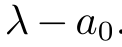
\includegraphics[width=34.42pt]{images-full/p047-i010.png}}\allowbreak{}.
困县型八州树例削
\par\medskip\noindent\textbf{【例1.2.42 】设\allowbreak{}\raisebox{-1.68pt}{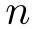
\includegraphics[width=10.17pt]{images-full/p047-i011.png}}\allowbreak{} 阶实方阵\allowbreak{}\raisebox{-2.76pt}{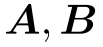
\includegraphics[width=28.81pt]{images-full/p047-i012.png}}\allowbreak{} 满足\allowbreak{}\raisebox{-3.00pt}{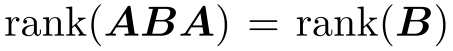
\includegraphics[width=127.69pt]{images-full/p047-i013.png}}\allowbreak{} 证明:\allowbreak{}\raisebox{-2.28pt}{
\includegraphics[width=23.16pt]{images-full/p047-i014.png}}\allowbreak{} 与}
\allowbreak{}\raisebox{-2.28pt}{
\includegraphics[width=23.73pt]{images-full/p047-i015.png}}\allowbreak{} 相似.
\par\noindent\textbf{证明}\ 设\allowbreak{}\raisebox{-3.00pt}{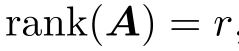
\includegraphics[width=67.18pt]{images-full/p047-i016.png}}\allowbreak{}，且设
\sourceblock{373.46}{images-full/p047-d003.png}
\sourceblock{301.14}{images-full/p047-d004.png}


% SOURCE_PDF_PAGE 48

\hypertarget{source-p048}{}
\sourceblock{323.74}{images-full/p048-d000.png}
\sourceblock{298.88}{images-full/p048-d001.png}
从而有
\sourceblock{372.90}{images-full/p048-d002.png}
【点i平】此题表面上看是矩阵相似的判定问题，实质是矩阵的等价标准形的应用.当
然也还需要利用分块矩阵技巧.
\sourceblock{450.00}{images-full/p048-d003.png}


% SOURCE_PDF_PAGE 49

\hypertarget{source-p049}{}
如秩、迹、行列式、特征值等.此外，不变因子组和初等因子组也都是矩阵的相似不变量，
而且由于初等因子组唯一地决定了Jor也且标准形，从而$A$ 与$B$ 相似又等价于$A$ 与$B$
杳相同的初等因子组，也等价于$A$与$B$ 有相同的不变因子组.
\par\medskip\noindent\textbf{【例1.2.44 】设实对称矩阵}
\sourceblock{98.87}{images-full/p049-d000.png}
\sourceblock{280.80}{images-full/p049-d001.png}
相似，求\allowbreak{}\raisebox{-2.16pt}{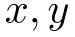
\includegraphics[width=20.90pt]{images-full/p049-i006.png}}\allowbreak{} 及满足\allowbreak{}\raisebox{-3.24pt}{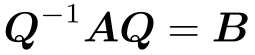
\includegraphics[width=71.75pt]{images-full/p049-i007.png}}\allowbreak{} 的正交矩阵\allowbreak{}\raisebox{-2.76pt}{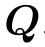
\includegraphics[width=12.65pt]{images-full/p049-i008.png}}\allowbreak{}
解$A$ 与$B$ 相似=\allowbreak{}\raisebox{-2.40pt}{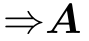
\includegraphics[width=24.86pt]{images-full/p049-i011.png}}\allowbreak{} 与$B$ 有相同的迹和行列式.进而得
\sourceblock{128.25}{images-full/p049-d002.png}
\sourceblock{428.27}{images-full/p049-d003.png}


% SOURCE_PDF_PAGE 50

\hypertarget{source-p050}{}
\sourceblock{393.24}{images-full/p050-d000.png}
\sourceblock{276.85}{images-full/p050-d001.png}
\sourceblock{397.19}{images-full/p050-d002.png}
\sourceblock{436.74}{images-full/p050-d003.png}
C 使得$A$ 相似于
\sourceblock{110.74}{images-full/p050-d004.png}
\par\noindent\textbf{证明}\ (1) 由署等阵可对角化，且其特征值\allowbreak{}\raisebox{-2.76pt}{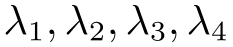
\includegraphics[width=65.54pt]{images-full/p050-i001.png}}\allowbreak{} 要么为1，要么为0，因此有
\sourceblock{146.90}{images-full/p050-d005.png}


% SOURCE_PDF_PAGE 51

\hypertarget{source-p051}{}
\sourceblock{266.11}{images-full/p051-d000.png}
\sourceblock{450.00}{images-full/p051-d001.png}
\sourceblock{298.88}{images-full/p051-d002.png}
考察关于句\allowbreak{}\raisebox{-2.04pt}{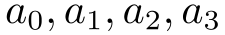
\includegraphics[width=63.28pt]{images-full/p051-i000.png}}\allowbreak{}的线性方程组:
\sourceblock{428.83}{images-full/p051-d003.png}
\sourceblock{159.33}{images-full/p051-d004.png}
则有\allowbreak{}\raisebox{-3.00pt}{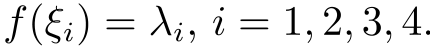
\includegraphics[width=121.02pt]{images-full/p051-i001.png}}\allowbreak{} 所以
\sourceblock{398.32}{images-full/p051-d005.png}
\sourceblock{383.07}{images-full/p051-d006.png}


% SOURCE_PDF_PAGE 52

\hypertarget{source-p052}{}
因此本题获证.口
\phantomsection\addcontentsline{toc}{section}{1.3 真题选讲与点评}
\par 4 u 真题选讲与点评\}-
\par\medskip\noindent\textbf{【例1.3.1 】(第四届全国初赛题{\symbolfont ①})已知实矩阵}
\sourceblock{185.88}{images-full/p053-d002.png}
\sourceblock{447.48}{images-full/p053-d003.png}
\par\noindent\textbf{证明}\ (l)\allowbreak{}\raisebox{-2.28pt}{
\includegraphics[width=50.28pt]{images-full/p053-i005.png}}\allowbreak{} 有解等价于$B$ 的列向量组可由$A$ 的列向量组线性表示. \allowbreak{}\raisebox{-2.28pt}{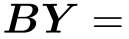
\includegraphics[width=36.16pt]{images-full/p053-i008.png}}\allowbreak{}
$A$无解等价于$A$ 的某个列向量不能由$B$ 的列向量组线性表示.对\allowbreak{}\raisebox{-3.00pt}{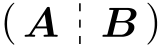
\includegraphics[width=46.33pt]{images-full/p053-i012.png}}\allowbreak{} 作初等变换
\sourceblock{311.31}{images-full/p053-d004.png}
\sourceblock{371.77}{images-full/p053-d005.png}
{\symbolfont ①}第四届全国太学生数学竞赛初赛数学专业组试题简写为第四届全国初赛题.以下为方便叙述，数学专业组试题全部
按这种格式简写，非数学专业组试题按照第四届全国初赛题(非数学类)的格式标记.


% SOURCE_PDF_PAGE 54

\hypertarget{source-p054}{}
而若\allowbreak{}\raisebox{-2.88pt}{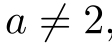
\includegraphics[width=31.21pt]{images-full/p054-i000.png}}\allowbreak{}，则$A$ 的列向量组线性无关.$B$ 的两个列向量都可以由$A$ 的列向量组线
性表示.所以\allowbreak{}\raisebox{-2.28pt}{
\includegraphics[width=51.41pt]{images-full/p054-i004.png}}\allowbreak{}有解的充要条件是\allowbreak{}\raisebox{-2.76pt}{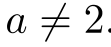
\includegraphics[width=31.03pt]{images-full/p054-i005.png}}\allowbreak{}
类似地，对\allowbreak{}\raisebox{-3.00pt}{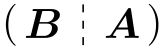
\includegraphics[width=46.89pt]{images-full/p054-i006.png}}\allowbreak{}作初等变换
\sourceblock{450.00}{images-full/p054-d000.png}
\allowbreak{}\raisebox{-3.00pt}{
\includegraphics[width=51.64pt]{images-full/p054-i007.png}}\allowbreak{}，即
\sourceblock{176.84}{images-full/p054-d001.png}
\sourceblock{323.18}{images-full/p054-d002.png}
$A$ 和$B$ 的特征多项式均为\allowbreak{}\raisebox{-3.12pt}{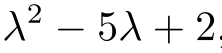
\includegraphics[width=62.38pt]{images-full/p054-i010.png}}\allowbreak{}，它有两个互不相等的实根\allowbreak{}\raisebox{-2.76pt}{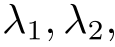
\includegraphics[width=32.29pt]{images-full/p054-i011.png}}\allowbreak{}，所以$A$ 与$B$
\sourceblock{450.00}{images-full/p054-d003.png}
\sourceblock{265.55}{images-full/p054-d004.png}
所以\allowbreak{}\raisebox{-3.00pt}{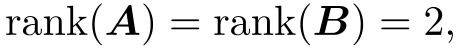
\includegraphics[width=128.49pt]{images-full/p054-i014.png}}\allowbreak{}，且$A$ 的正负惯性指数也都是1.
易知$A$ 的一个合同标准形为
\sourceblock{450.00}{images-full/p054-d005.png}


% SOURCE_PDF_PAGE 55

\hypertarget{source-p055}{}
\par\medskip\noindent\textbf{【例1.3.2 】(第七届全国初赛题)设$A$ 为$n$ 阶方阵其$n$个特征值均为偶数. 证明}
关于$X$ 的矩阵方程
\sourceblock{119.78}{images-full/p055-d000.png}
\sourceblock{209.05}{images-full/p055-d001.png}
\sourceblock{104.52}{images-full/p055-d002.png}
设\allowbreak{}\raisebox{-3.24pt}{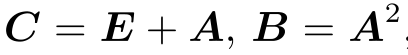
\includegraphics[width=115.05pt]{images-full/p055-i004.png}}\allowbreak{}，且$A$ 的$n$个特征值为\allowbreak{}\raisebox{-2.76pt}{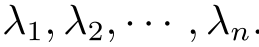
\includegraphics[width=72.78pt]{images-full/p055-i007.png}}\allowbreak{} 则$C$ 的$n$个特征
值为
\sourceblock{136.73}{images-full/p055-d003.png}
$B$ 的$n$个特征值为
\sourceblock{310.18}{images-full/p055-d004.png}
\sourceblock{311.31}{images-full/p055-d005.png}
以此类推.对任意的正整数$k$ 有\allowbreak{}\raisebox{-2.88pt}{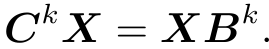
\includegraphics[width=75.52pt]{images-full/p055-i013.png}}\allowbreak{}•
设$C$ 的特征多项式为
\sourceblock{406.80}{images-full/p055-d006.png}
\sourceblock{216.96}{images-full/p055-d007.png}
\sourceblock{154.81}{images-full/p055-d008.png}
由于\allowbreak{}\raisebox{-3.24pt}{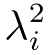
\includegraphics[width=14.12pt]{images-full/p055-i015.png}}\allowbreak{} 为偶数，\allowbreak{}\raisebox{-3.00pt}{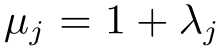
\includegraphics[width=62.71pt]{images-full/p055-i016.png}}\allowbreak{} 为奇数.所以\allowbreak{}\raisebox{-3.00pt}{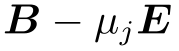
\includegraphics[width=50.28pt]{images-full/p055-i017.png}}\allowbreak{} 的特征值均不等于\allowbreak{}\raisebox{-2.28pt}{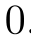
\includegraphics[width=8.43pt]{images-full/p055-i018.png}}\allowbreak{}. 故\allowbreak{}\raisebox{-3.00pt}{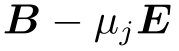
\includegraphics[width=50.28pt]{images-full/p055-i019.png}}\allowbreak{}
可逆.由此得到\allowbreak{}\raisebox{-2.40pt}{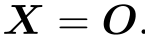
\includegraphics[width=40.63pt]{images-full/p055-i020.png}}\allowbreak{}口
\par\medskip\noindent\textbf{【例1.3.31 (第八届全国初赛题)设\allowbreak{}\raisebox{-2.76pt}{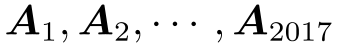
\includegraphics[width=95.48pt]{images-full/p055-i021.png}}\allowbreak{} 为2016 阶实方阵证明: 关}
于\allowbreak{}\raisebox{-2.16pt}{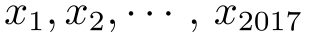
\includegraphics[width=87.01pt]{images-full/p055-i022.png}}\allowbreak{} 的方程
\sourceblock{218.09}{images-full/p055-d009.png}


% SOURCE_PDF_PAGE 56

\hypertarget{source-p056}{}
至少有一组非零实数解，其中det 表示行列式.
\sourceblock{389.85}{images-full/p056-d000.png}
\sourceblock{208.48}{images-full/p056-d001.png}
这个方程组有2016 个方程、2017 个未知数.所以它有非零解.设\allowbreak{}\raisebox{-2.16pt}{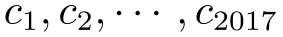
\includegraphics[width=79.66pt]{images-full/p056-i000.png}}\allowbreak{} 是它的
一组非零解.这表明
\sourceblock{163.28}{images-full/p056-d002.png}
的第\allowbreak{}\raisebox{-2.28pt}{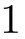
\includegraphics[width=6.78pt]{images-full/p056-i001.png}}\allowbreak{}列为零向量.从而
\sourceblock{215.83}{images-full/p056-d003.png}
故\allowbreak{}\raisebox{-2.04pt}{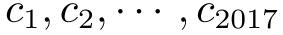
\includegraphics[width=79.66pt]{images-full/p056-i002.png}}\allowbreak{} 是方程
\sourceblock{218.09}{images-full/p056-d004.png}
的一组非零实数解.口
\par\medskip\noindent\textbf{【例1.3.4】(第九届全国初赛题)设\allowbreak{}\raisebox{-3.12pt}{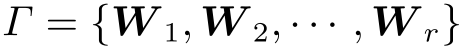
\includegraphics[width=131.64pt]{images-full/p056-i003.png}}\allowbreak{} 为$T$个互不相同的可}
逆$n$阶复方阵构成的集合若该集合关于矩阵乘法封闭(即\allowbreak{}\raisebox{-2.76pt}{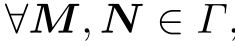
\includegraphics[width=66.14pt]{images-full/p056-i006.png}}\allowbreak{}，有\allowbreak{}\raisebox{-2.97pt}{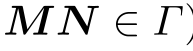
\includegraphics[width=54.36pt]{images-full/p056-i007.png}}\allowbreak{}.
\par\noindent\textbf{证明}\ 
\sourceblock{206.22}{images-full/p056-d005.png}
\sourceblock{361.03}{images-full/p056-d006.png}
\sourceblock{218.09}{images-full/p056-d007.png}
又\allowbreak{}\raisebox{-2.28pt}{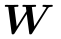
\includegraphics[width=16.95pt]{images-full/p056-i008.png}}\allowbreak{} 可逆，若研rwi=wwj ，则奋阴气=Wj . 这表明\allowbreak{}\raisebox{-2.28pt}{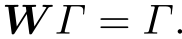
\includegraphics[width=51.03pt]{images-full/p056-i009.png}}\allowbreak{}.
\sourceblock{235.04}{images-full/p056-d008.png}
\sourceblock{257.64}{images-full/p056-d009.png}
即\allowbreak{}\raisebox{-2.88pt}{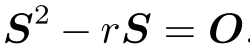
\includegraphics[width=70.26pt]{images-full/p056-i010.png}}\allowbreak{} 若\allowbreak{}\raisebox{-2.28pt}{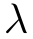
\includegraphics[width=9.04pt]{images-full/p056-i011.png}}\allowbreak{} 为$S$ 的一个特征值，则有\allowbreak{}\raisebox{-2.76pt}{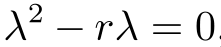
\includegraphics[width=62.07pt]{images-full/p056-i013.png}}\allowbreak{}，即\allowbreak{}\raisebox{-2.28pt}{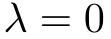
\includegraphics[width=31.07pt]{images-full/p056-i014.png}}\allowbreak{} 或\allowbreak{}\raisebox{-2.28pt}{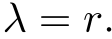
\includegraphics[width=31.43pt]{images-full/p056-i015.png}}\allowbreak{}.这表明
$S$ 的特征值只可能为0 或\allowbreak{}\raisebox{-1.56pt}{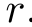
\includegraphics[width=8.72pt]{images-full/p056-i017.png}}\allowbreak{}


% SOURCE_PDF_PAGE 57

\hypertarget{source-p057}{}
\sourceblock{450.00}{images-full/p057-d000.png}
\par\medskip\noindent\textbf{【例1.3.5] (第九届全国初赛题)给定非霉实数\allowbreak{}\raisebox{-1.56pt}{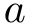
\includegraphics[width=9.04pt]{images-full/p057-i000.png}}\allowbreak{} 及\allowbreak{}\raisebox{-1.56pt}{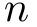
\includegraphics[width=10.17pt]{images-full/p057-i001.png}}\allowbreak{} 阶实反对称矩阵A. 记}
\sourceblock{250.29}{images-full/p057-d001.png}
\par\noindent\textbf{证明}\ 任取$T$ 中两个元素\allowbreak{}\raisebox{-2.88pt}{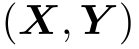
\includegraphics[width=38.98pt]{images-full/p057-i003.png}}\allowbreak{} 和\allowbreak{}\raisebox{-3.00pt}{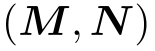
\includegraphics[width=43.50pt]{images-full/p057-i004.png}}\allowbreak{} 必有
\sourceblock{110.74}{images-full/p057-d002.png}
\par\noindent\textbf{证明}\ 反证法.若存在\allowbreak{}\raisebox{-3.00pt}{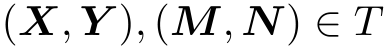
\includegraphics[width=110.17pt]{images-full/p057-i005.png}}\allowbreak{}使得
\sourceblock{110.74}{images-full/p057-d003.png}
则有
\sourceblock{110.74}{images-full/p057-d004.png}
因为\allowbreak{}\raisebox{-3.36pt}{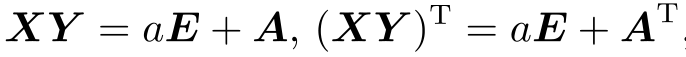
\includegraphics[width=193.69pt]{images-full/p057-i006.png}}\allowbreak{}，又\allowbreak{}\raisebox{-3.24pt}{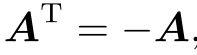
\includegraphics[width=55.36pt]{images-full/p057-i007.png}}\allowbreak{}，所以
\sourceblock{120.34}{images-full/p057-d005.png}
\sourceblock{268.38}{images-full/p057-d006.png}
因此
\sourceblock{378.55}{images-full/p057-d007.png}
\sourceblock{331.65}{images-full/p057-d008.png}
\sourceblock{450.00}{images-full/p057-d009.png}
\allowbreak{}\raisebox{-2.76pt}{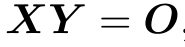
\includegraphics[width=52.04pt]{images-full/p057-i008.png}}\allowbreak{}，与\allowbreak{}\raisebox{-2.76pt}{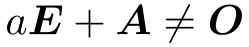
\includegraphics[width=70.06pt]{images-full/p057-i009.png}}\allowbreak{} 矛盾.口


% SOURCE_PDF_PAGE 58

\hypertarget{source-p058}{}
\par\medskip\noindent\textbf{【例1.3.6】(第八届全国初赛题)设$n$ 为奇数，\allowbreak{}\raisebox{-2.76pt}{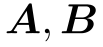
\includegraphics[width=28.81pt]{images-full/p058-i001.png}}\allowbreak{} 为两个$n$阶实方阵且\allowbreak{}\raisebox{-2.40pt}{
\includegraphics[width=50.29pt]{images-full/p058-i003.png}}\allowbreak{}}
记\allowbreak{}\raisebox{-2.64pt}{
\includegraphics[width=44.63pt]{images-full/p058-i004.png}}\allowbreak{} 的特征值集舍为\allowbreak{}\raisebox{-2.64pt}{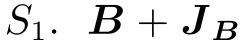
\includegraphics[width=68.93pt]{images-full/p058-i005.png}}\allowbreak{} 的特征值集合为\allowbreak{}\raisebox{-2.76pt}{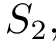
\includegraphics[width=15.61pt]{images-full/p058-i006.png}}\allowbreak{}其中\allowbreak{}\raisebox{-2.76pt}{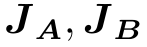
\includegraphics[width=41.24pt]{images-full/p058-i007.png}}\allowbreak{} 分别表示
\allowbreak{}\raisebox{-2.76pt}{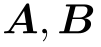
\includegraphics[width=28.25pt]{images-full/p058-i008.png}}\allowbreak{} 的Jordan 标准形.证明:\allowbreak{}\raisebox{-2.64pt}{\includegraphics[width=61.28pt]{images-full/p058-i009.png}}\allowbreak{}.
\par\noindent\textbf{证明}\ \allowbreak{}\raisebox{-2.76pt}{\includegraphics[width=61.61pt]{images-full/p058-i010.png}}\allowbreak{}，即\allowbreak{}\raisebox{-2.28pt}{\includegraphics[width=9.04pt]{images-full/p058-i011.png}}\allowbreak{} 为\allowbreak{}\raisebox{-2.76pt}{\includegraphics[width=43.50pt]{images-full/p058-i012.png}}\allowbreak{} 或者\allowbreak{}\raisebox{-2.64pt}{\includegraphics[width=44.63pt]{images-full/p058-i013.png}}\allowbreak{} 的特征值或等价地\allowbreak{}\raisebox{-2.76pt}{\includegraphics[width=43.50pt]{images-full/p058-i014.png}}\allowbreak{} 或者
\sourceblock{345.78}{images-full/p058-d000.png}
\sourceblock{276.28}{images-full/p058-d001.png}
\sourceblock{433.92}{images-full/p058-d002.png}
\sourceblock{276.28}{images-full/p058-d003.png}
解对$B$ 进行初等变换:
\sourceblock{262.72}{images-full/p058-d004.png}
\sourceblock{330.52}{images-full/p058-d005.png}
注意到$A$ 是可逆反对称矩阵，故有
\sourceblock{224.87}{images-full/p058-d006.png}
\sourceblock{368.38}{images-full/p058-d007.png}
由此得\allowbreak{}\raisebox{-3.24pt}{\includegraphics[width=75.28pt]{images-full/p058-i017.png}}\allowbreak{}，故\allowbreak{}\raisebox{-3.00pt}{\includegraphics[width=69.58pt]{images-full/p058-i018.png}}\allowbreak{}
【点评】此题考察的是矩阵秩的计算问题.由于$B$ 是分块形式，因此使用分块初等
变换是自然的.
\par\medskip\noindent\textbf{【例1.3.8] (第二届全国决赛题)设\allowbreak{}\raisebox{-3.12pt}{\includegraphics[width=87.57pt]{images-full/p058-i020.png}}\allowbreak{}是数域$F$上两个矩阵集合，称}
它们在$F$上相似，如果存在$F$上与\allowbreak{}\raisebox{-2.28pt}{\includegraphics[width=27.68pt]{images-full/p058-i024.png}}\allowbreak{}无关的可逆矩阵$P$，使得\allowbreak{}\raisebox{-3.24pt}{\includegraphics[width=116.95pt]{images-full/p058-i026.png}}\allowbreak{}


% SOURCE_PDF_PAGE 59

\hypertarget{source-p059}{}
\par\noindent\textbf{证明}\ :对有理数域$Q$ 上的两个矩阵集合\allowbreak{}\raisebox{-3.12pt}{\includegraphics[width=92.09pt]{images-full/p059-i001.png}}\allowbreak{} ，如果它们在实数域$R$ 上相
似，则它们在有理数域$Q$ 上也相似.
\par\noindent\textbf{证明}\ \allowbreak{}\raisebox{-2.64pt}{\includegraphics[width=36.55pt]{images-full/p059-i004.png}}\allowbreak{}考虑\allowbreak{}\raisebox{-3.00pt}{\includegraphics[width=37.29pt]{images-full/p059-i005.png}}\allowbreak{} 的子空间
\sourceblock{179.67}{images-full/p059-d000.png}
以及\allowbreak{}\raisebox{-3.00pt}{\includegraphics[width=37.85pt]{images-full/p059-i006.png}}\allowbreak{} 的子空间
\sourceblock{180.80}{images-full/p059-d001.png}
其中\allowbreak{}\raisebox{-3.00pt}{\includegraphics[width=80.23pt]{images-full/p059-i007.png}}\allowbreak{} 分别表示实数域$R$和有理数域$Q$ 上全体$n$ 阶矩阵构成的向量空间.
令
\sourceblock{155.37}{images-full/p059-d002.png}
由题意知\allowbreak{}\raisebox{-3.12pt}{\includegraphics[width=49.80pt]{images-full/p059-i011.png}}\allowbreak{} 由于所涉及的向量空间维数均不超过\allowbreak{}\raisebox{-3.12pt}{\includegraphics[width=14.19pt]{images-full/p059-i012.png}}\allowbreak{}，故\allowbreak{}\raisebox{-2.64pt}{\includegraphics[width=16.38pt]{images-full/p059-i013.png}}\allowbreak{} 和\allowbreak{}\raisebox{-2.88pt}{\includegraphics[width=22.60pt]{images-full/p059-i014.png}}\allowbreak{} 的基实际土
就是线性方程组(这些方程由\allowbreak{}\raisebox{-2.76pt}{\includegraphics[width=66.10pt]{images-full/p059-i015.png}}\allowbreak{}给出)的基础解系.而求它们的基础解系的步
骤相同，因此可以取到一组公共基，设为\allowbreak{}\raisebox{-2.76pt}{\includegraphics[width=79.39pt]{images-full/p059-i016.png}}\allowbreak{} 考虑多项式
\sourceblock{180.80}{images-full/p059-d003.png}
由\allowbreak{}\raisebox{-2.64pt}{\includegraphics[width=16.38pt]{images-full/p059-i017.png}}\allowbreak{}含实可逆矩阵可知，存在一组实数\allowbreak{}\raisebox{-2.16pt}{\includegraphics[width=65.54pt]{images-full/p059-i018.png}}\allowbreak{}满足
\sourceblock{106.78}{images-full/p059-d004.png}
这表明$f$ 作为$Q$上的多项式不是零多项式，因此存在一组有理数\allowbreak{}\raisebox{-2.16pt}{\includegraphics[width=64.97pt]{images-full/p059-i021.png}}\allowbreak{}使得
\sourceblock{106.78}{images-full/p059-d005.png}
此时
\sourceblock{102.83}{images-full/p059-d006.png}
\sourceblock{450.00}{images-full/p059-d007.png}
【点评】此题讨论的是一组矩阵同时相似变换的问题.平时习题中讨论的多是一
组矩阵同时对角化的问题.同时相似变换或同时合同变换到我们给定的特殊形状的矩阵，
在工程应用中往往发挥着重要的作用.事实上，广义Schur 分解也属于此范畴(所谓广义
Schur 分解是指\allowbreak{}\raisebox{-3.00pt}{\includegraphics[width=86.49pt]{images-full/p059-i022.png}}\allowbreak{}，则必存在国阵$Q$ 和$Z$ 使得\allowbreak{}\raisebox{-3.00pt}{\includegraphics[width=38.42pt]{images-full/p059-i025.png}}\allowbreak{} 与\allowbreak{}\raisebox{-3.00pt}{\includegraphics[width=38.98pt]{images-full/p059-i026.png}}\allowbreak{} 均为上
三角阵，这里\allowbreak{}\raisebox{-2.88pt}{\includegraphics[width=16.95pt]{images-full/p059-i027.png}}\allowbreak{}表示$Q$ 的共辄转置).


% SOURCE_PDF_PAGE 60

\hypertarget{source-p060}{}
\sourceblock{450.00}{images-full/p060-d000.png}
其中\allowbreak{}\raisebox{-2.64pt}{\includegraphics[width=17.51pt]{images-full/p060-i000.png}}\allowbreak{} 为$T$ 阶单位矩阵
\sourceblock{302.84}{images-full/p060-d001.png}
又由\allowbreak{}\raisebox{-3.24pt}{\includegraphics[width=44.40pt]{images-full/p060-i002.png}}\allowbreak{}，有
\sourceblock{250.29}{images-full/p060-d002.png}
\sourceblock{403.97}{images-full/p060-d003.png}
故有
\sourceblock{137.86}{images-full/p060-d004.png}
\sourceblock{450.00}{images-full/p060-d005.png}


% SOURCE_PDF_PAGE 61

\hypertarget{source-p061}{}
\sourceblock{381.37}{images-full/p061-d000.png}
【点评】此题考察的焦点是与矩阵秩相关联的等价标准形以及分块矩阵的乘法运
算.事实上，本题若利用矩阵的Jordan 标准形，则能豆加直接地得到答案.
\par\medskip\noindent\textbf{【例1.3.10】(第九届全国决赛题(非数学类))设\allowbreak{}\raisebox{-2.76pt}{\includegraphics[width=41.24pt]{images-full/p061-i000.png}}\allowbreak{}是互不相同的正实数，}
\allowbreak{}\raisebox{-2.16pt}{\includegraphics[width=46.33pt]{images-full/p061-i001.png}}\allowbreak{} 是实数，满足
\sourceblock{234.47}{images-full/p061-d001.png}
\sourceblock{287.02}{images-full/p061-d002.png}
的值.
解将所给四个等式取对数，得到以\allowbreak{}\raisebox{-2.76pt}{\includegraphics[width=89.27pt]{images-full/p061-i002.png}}\allowbreak{} 为解的线性方程组;
\sourceblock{149.16}{images-full/p061-d003.png}
\sourceblock{450.00}{images-full/p061-d004.png}
为o (Cramer 法则)，即所求的行列式为O.
【点评】此题为典型的利用行列式性质求行列式值的问题，其关键技巧在于巧妙地
将现有条件转化为线性方程组有非零解，从而使用Cramer 法则迅速得到结果.
\par\medskip\noindent\textbf{【例1.3.11)(第八届全国决赛题(非数学类))设$n$ 阶方阵\allowbreak{}\raisebox{-2.76pt}{\includegraphics[width=28.81pt]{images-full/p061-i004.png}}\allowbreak{}满足\allowbreak{}\raisebox{-2.76pt}{\includegraphics[width=72.64pt]{images-full/p061-i005.png}}\allowbreak{}，}
\par\noindent\textbf{证明}\ :若存在正整数$k$ 使得\allowbreak{}\raisebox{-3.24pt}{\includegraphics[width=44.38pt]{images-full/p061-i007.png}}\allowbreak{}，则有行列式\allowbreak{}\raisebox{-3.00pt}{\includegraphics[width=101.51pt]{images-full/p061-i008.png}}\allowbreak{}


% SOURCE_PDF_PAGE 62

\hypertarget{source-p062}{}
\par\noindent\textbf{证明}\ 由\allowbreak{}\raisebox{-2.88pt}{\includegraphics[width=44.63pt]{images-full/p062-i000.png}}\allowbreak{} 知\allowbreak{}\raisebox{-3.00pt}{\includegraphics[width=41.43pt]{images-full/p062-i001.png}}\allowbreak{} 又由\allowbreak{}\raisebox{-2.52pt}{\includegraphics[width=75.14pt]{images-full/p062-i002.png}}\allowbreak{} 得
\sourceblock{398.32}{images-full/p062-d000.png}
再次由\allowbreak{}\raisebox{-2.52pt}{\includegraphics[width=76.27pt]{images-full/p062-i003.png}}\allowbreak{} 可得\allowbreak{}\raisebox{-3.00pt}{\includegraphics[width=84.50pt]{images-full/p062-i004.png}}\allowbreak{}，从丽\allowbreak{}\raisebox{-3.00pt}{\includegraphics[width=93.14pt]{images-full/p062-i005.png}}\allowbreak{} 因\allowbreak{}\raisebox{-3.24pt}{\includegraphics[width=45.90pt]{images-full/p062-i006.png}}\allowbreak{}，从而
$A$ 的特征值皆为\allowbreak{}\raisebox{-2.64pt}{\includegraphics[width=51.41pt]{images-full/p062-i008.png}}\allowbreak{} 的特征值皆为\allowbreak{}\raisebox{-2.16pt}{\includegraphics[width=15.91pt]{images-full/p062-i009.png}}\allowbreak{} ，因此有\allowbreak{}\raisebox{-3.00pt}{\includegraphics[width=65.22pt]{images-full/p062-i010.png}}\allowbreak{}，进而\allowbreak{}\raisebox{-3.00pt}{\includegraphics[width=41.37pt]{images-full/p062-i011.png}}\allowbreak{}，所以
\sourceblock{280.24}{images-full/p062-d001.png}
【点评】此题考察的仍是行列式的计算问题.利用的主要知识点是:方阵的行列式
等于该方阵的特征值之积.
\par\medskip\noindent\textbf{【例1.3.12 】(第五届全国决赛题(非数学类))设矩阵}
\sourceblock{106.22}{images-full/p062-d002.png}
其中\allowbreak{}\raisebox{-1.68pt}{\includegraphics[width=9.04pt]{images-full/p062-i012.png}}\allowbreak{}为常数，矩阵$B$ 满足关系式\allowbreak{}\raisebox{-2.88pt}{\includegraphics[width=102.26pt]{images-full/p062-i014.png}}\allowbreak{}其中$E$ 为单位矩阵，且\allowbreak{}\raisebox{-2.76pt}{\includegraphics[width=40.20pt]{images-full/p062-i016.png}}\allowbreak{}
试求常数\allowbreak{}\raisebox{-1.68pt}{\includegraphics[width=9.04pt]{images-full/p062-i017.png}}\allowbreak{} 的值.
解由\allowbreak{}\raisebox{-2.52pt}{\includegraphics[width=100.57pt]{images-full/p062-i018.png}}\allowbreak{}得\allowbreak{}\raisebox{-3.00pt}{\includegraphics[width=108.82pt]{images-full/p062-i019.png}}\allowbreak{} 再由\allowbreak{}\raisebox{-2.76pt}{\includegraphics[width=39.55pt]{images-full/p062-i020.png}}\allowbreak{} 知$A+E$ 必为不
可逆矩阵，从而\allowbreak{}\raisebox{-3.00pt}{\includegraphics[width=65.19pt]{images-full/p062-i022.png}}\allowbreak{} 直接计算可知
\sourceblock{198.31}{images-full/p062-d003.png}
\sourceblock{450.00}{images-full/p062-d004.png}
等价定义即可解此题.
\par\medskip\noindent\textbf{【例1.3.13 】(第六届全国决赛题(非数学类))设\allowbreak{}\raisebox{-2.76pt}{\includegraphics[width=80.23pt]{images-full/p062-i023.png}}\allowbreak{} 皆为$n$ 阶方阵，其}
中\allowbreak{}\raisebox{-2.76pt}{\includegraphics[width=38.42pt]{images-full/p062-i025.png}}\allowbreak{} 可逆.证明:存在可逆矩阵\allowbreak{}\raisebox{-2.76pt}{\includegraphics[width=28.81pt]{images-full/p062-i026.png}}\allowbreak{} 使得
\sourceblock{124.86}{images-full/p062-d005.png}
成立的充要条件是\allowbreak{}\raisebox{-3.36pt}{\includegraphics[width=38.98pt]{images-full/p062-i027.png}}\allowbreak{}与\allowbreak{}\raisebox{-3.36pt}{\includegraphics[width=40.68pt]{images-full/p062-i028.png}}\allowbreak{}相似.
\par\noindent\textbf{证明}\ 必要性由条件得\allowbreak{}\raisebox{-3.36pt}{\includegraphics[width=192.03pt]{images-full/p062-i029.png}}\allowbreak{} 因此有
\sourceblock{251.42}{images-full/p062-d006.png}
即有\allowbreak{}\raisebox{-3.36pt}{\includegraphics[width=39.55pt]{images-full/p062-i030.png}}\allowbreak{} 与\allowbreak{}\raisebox{-3.36pt}{\includegraphics[width=40.68pt]{images-full/p062-i031.png}}\allowbreak{}相似.


% SOURCE_PDF_PAGE 63

\hypertarget{source-p063}{}
充分性由\allowbreak{}\raisebox{-3.36pt}{\includegraphics[width=39.55pt]{images-full/p063-i000.png}}\allowbreak{}与\allowbreak{}\raisebox{-3.36pt}{\includegraphics[width=40.68pt]{images-full/p063-i001.png}}\allowbreak{}相似知，存在可逆矩阵$P$使得
\sourceblock{131.08}{images-full/p063-d000.png}
\sourceblock{284.19}{images-full/p063-d001.png}
令\allowbreak{}\raisebox{-3.36pt}{\includegraphics[width=90.40pt]{images-full/p063-i003.png}}\allowbreak{} 则有\allowbreak{}\raisebox{-3.24pt}{\includegraphics[width=82.78pt]{images-full/p063-i004.png}}\allowbreak{} 即\allowbreak{}\raisebox{-2.76pt}{\includegraphics[width=70.48pt]{images-full/p063-i005.png}}\allowbreak{}•
另一方面，有\allowbreak{}\raisebox{-3.36pt}{\includegraphics[width=178.26pt]{images-full/p063-i006.png}}\allowbreak{}口
【点评】此题表面上看是考察两个矩阵同时等价的问题，实质上只需熟练掌握可逆
矩阵的基本性质即可.
\par\medskip\noindent\textbf{【例1.3.14】(第七届全国决赛题(非数学类))设$A$ 是\allowbreak{}\raisebox{-1.80pt}{\includegraphics[width=34.46pt]{images-full/p063-i008.png}}\allowbreak{} 矩阵，$B$ 是\allowbreak{}\raisebox{-2.28pt}{\includegraphics[width=30.19pt]{images-full/p063-i010.png}}\allowbreak{} 矩}
阵，$C$ 是\allowbreak{}\raisebox{-2.28pt}{\includegraphics[width=29.94pt]{images-full/p063-i012.png}}\allowbreak{}矩阵，证明:
\sourceblock{266.11}{images-full/p063-d002.png}
其中\allowbreak{}\raisebox{-3.00pt}{\includegraphics[width=46.89pt]{images-full/p063-i013.png}}\allowbreak{} 表示矩阵$X$ 的秩.
\par\noindent\textbf{证明}\ 欲证的不等式即
\sourceblock{392.67}{images-full/p063-d003.png}
注意到
\sourceblock{354.25}{images-full/p063-d004.png}
因此有
\sourceblock{392.67}{images-full/p063-d005.png}
\sourceblock{450.00}{images-full/p063-d006.png}
【点评】证明矩阵秩的不等式往往利用的是分块矩阵及分块初等变换不改变矩阵的
秩来完成的.本题是这一类型的典型代表.事实上，本题欲证的结论即著名的Frobeniu日
秩不等式.
\par\medskip\noindent\textbf{【例1.3.15 】(第十五届全国初赛题)证明对任意$n$ 阶方阵$A$，存在主对角线上元素}
为1 或\allowbreak{}\raisebox{-2.16pt}{\includegraphics[width=16.38pt]{images-full/p063-i017.png}}\allowbreak{} 的$n$ 阶对角矩阵$J$使得$A+J$ 可逆.


% SOURCE_PDF_PAGE 64

\hypertarget{source-p064}{}
\par\noindent\textbf{证明}\ 对$n$作归纳.当\allowbreak{}\raisebox{-2.28pt}{\includegraphics[width=30.51pt]{images-full/p064-i001.png}}\allowbreak{}时，\allowbreak{}\raisebox{-3.00pt}{\includegraphics[width=43.57pt]{images-full/p064-i002.png}}\allowbreak{}，显然\allowbreak{}\raisebox{-2.40pt}{\includegraphics[width=27.68pt]{images-full/p064-i003.png}}\allowbreak{}或者\allowbreak{}\raisebox{-2.28pt}{\includegraphics[width=27.68pt]{images-full/p064-i004.png}}\allowbreak{}中一定有一个数非
零，结论成立
设结论对\allowbreak{}\raisebox{-2.28pt}{\includegraphics[width=29.38pt]{images-full/p064-i005.png}}\allowbreak{}阶矩阵成立，下面考察$n$ 阶方阵\allowbreak{}\raisebox{-2.28pt}{\includegraphics[width=12.05pt]{images-full/p064-i007.png}}\allowbreak{} 记
\sourceblock{108.48}{images-full/p064-d000.png}
其中\allowbreak{}\raisebox{-2.64pt}{\includegraphics[width=16.95pt]{images-full/p064-i008.png}}\allowbreak{}为\allowbreak{}\raisebox{-2.16pt}{\includegraphics[width=29.38pt]{images-full/p064-i009.png}}\allowbreak{}阶矩阵，\allowbreak{}\raisebox{-1.68pt}{\includegraphics[width=11.30pt]{images-full/p064-i010.png}}\allowbreak{} 为\allowbreak{}\raisebox{-2.16pt}{\includegraphics[width=29.38pt]{images-full/p064-i011.png}}\allowbreak{}维行向量，\allowbreak{}\raisebox{-2.76pt}{\includegraphics[width=10.73pt]{images-full/p064-i012.png}}\allowbreak{} 为\allowbreak{}\raisebox{-2.16pt}{\includegraphics[width=29.38pt]{images-full/p064-i013.png}}\allowbreak{}维列向量，\allowbreak{}\raisebox{-2.04pt}{\includegraphics[width=20.34pt]{images-full/p064-i014.png}}\allowbreak{} 为一个数.由
归纳假设，存在主对角线上元素为\allowbreak{}\raisebox{-2.28pt}{\includegraphics[width=6.78pt]{images-full/p064-i015.png}}\allowbreak{}或\allowbreak{}\raisebox{-2.28pt}{\includegraphics[width=16.38pt]{images-full/p064-i016.png}}\allowbreak{} 的\allowbreak{}\raisebox{-2.28pt}{\includegraphics[width=29.38pt]{images-full/p064-i017.png}}\allowbreak{} 阶对角矩阵\allowbreak{}\raisebox{-2.64pt}{\includegraphics[width=15.25pt]{images-full/p064-i018.png}}\allowbreak{}使得\allowbreak{}\raisebox{-2.76pt}{\includegraphics[width=44.63pt]{images-full/p064-i019.png}}\allowbreak{}可逆.
从而
\sourceblock{253.12}{images-full/p064-d001.png}
这表明上式最左边的两个行列式中至少有一个非零.
\sourceblock{450.00}{images-full/p064-d002.png}
以结论对$n$ 阶矩阵成立.
\sourceblock{450.00}{images-full/p064-d003.png}
\sourceblock{450.00}{images-full/p064-d004.png}


% SOURCE_PDF_PAGE 65

\hypertarget{source-p065}{}
\sourceblock{356.51}{images-full/p065-d000.png}
\sourceblock{192.66}{images-full/p065-d001.png}
\sourceblock{268.38}{images-full/p065-d002.png}
\sourceblock{329.39}{images-full/p065-d003.png}
其中\allowbreak{}\raisebox{-2.76pt}{\includegraphics[width=45.11pt]{images-full/p065-i000.png}}\allowbreak{}注意到
\sourceblock{268.94}{images-full/p065-d004.png}
\sourceblock{297.19}{images-full/p065-d005.png}
\sourceblock{370.64}{images-full/p065-d006.png}
\sourceblock{371.20}{images-full/p065-d007.png}
\sourceblock{309.62}{images-full/p065-d008.png}
可知$A$ 的最小多项式\allowbreak{}\raisebox{-3.00pt}{\includegraphics[width=25.42pt]{images-full/p065-i002.png}}\allowbreak{} 只可能是下列\allowbreak{}\raisebox{-2.28pt}{\includegraphics[width=8.47pt]{images-full/p065-i003.png}}\allowbreak{}个多项式之一:
\sourceblock{380.24}{images-full/p065-d009.png}
\sourceblock{450.00}{images-full/p065-d010.png}


% SOURCE_PDF_PAGE 66

\hypertarget{source-p066}{}
\sourceblock{450.00}{images-full/p066-d000.png}
\sourceblock{168.93}{images-full/p066-d001.png}
\sourceblock{450.00}{images-full/p066-d002.png}
\sourceblock{104.52}{images-full/p066-d003.png}
可知\allowbreak{}\raisebox{-3.24pt}{\includegraphics[width=203.22pt]{images-full/p066-i000.png}}\allowbreak{}，因此$A$ 至多有两个非零特征值.故$A$ 的$n$
\sourceblock{270.63}{images-full/p066-d004.png}
所以\allowbreak{}\raisebox{-3.00pt}{\includegraphics[width=55.93pt]{images-full/p066-i004.png}}\allowbreak{} 的$n$个特征值为
\sourceblock{186.45}{images-full/p066-d005.png}
\sourceblock{389.28}{images-full/p066-d006.png}
\sourceblock{336.74}{images-full/p066-d007.png}


% SOURCE_PDF_PAGE 67

\hypertarget{source-p067}{}
其中
\sourceblock{342.95}{images-full/p067-d000.png}
利用行列式降阶公式，矩阵$A$ 的特征多项式可化为
\sourceblock{232.21}{images-full/p067-d001.png}
\sourceblock{378.55}{images-full/p067-d002.png}
\sourceblock{450.00}{images-full/p067-d003.png}
\sourceblock{413.01}{images-full/p067-d004.png}


% SOURCE_PDF_PAGE 68

\hypertarget{source-p068}{}
\sourceblock{412.45}{images-full/p068-d000.png}
\par\medskip\noindent\textbf{【例1.3.17】(第十四届全国初赛题)设矩阵}
\sourceblock{87.01}{images-full/p068-d001.png}
矩阵$B$ 与$A$ 可交换，其元素均为正整数且行列式为1.证明存在正整数$k$ 使得\allowbreak{}\raisebox{-2.76pt}{\includegraphics[width=45.79pt]{images-full/p068-i003.png}}\allowbreak{}
\par\noindent\textbf{证明}\ 令
\sourceblock{87.57}{images-full/p068-d002.png}
\sourceblock{450.00}{images-full/p068-d003.png}
若\allowbreak{}\raisebox{-2.76pt}{\includegraphics[width=30.62pt]{images-full/p068-i004.png}}\allowbreak{}则由\allowbreak{}\raisebox{-2.76pt}{\includegraphics[width=85.31pt]{images-full/p068-i005.png}}\allowbreak{}易得\allowbreak{}\raisebox{-2.64pt}{\includegraphics[width=32.09pt]{images-full/p068-i006.png}}\allowbreak{}，困此
\sourceblock{409.06}{images-full/p068-d004.png}
\sourceblock{450.00}{images-full/p068-d005.png}
\sourceblock{237.86}{images-full/p068-d006.png}


% SOURCE_PDF_PAGE 69

\hypertarget{source-p069}{}
中的元素\allowbreak{}\raisebox{-2.76pt}{\includegraphics[width=28.81pt]{images-full/p069-i000.png}}\allowbreak{}也满足矩阵$B$ 中元素\allowbreak{}\raisebox{-2.76pt}{\includegraphics[width=19.21pt]{images-full/p069-i002.png}}\allowbreak{}所满足的条件，但是\allowbreak{}\raisebox{-2.64pt}{\includegraphics[width=61.73pt]{images-full/p069-i003.png}}\allowbreak{} 继续进行下
去，通过左乘\allowbreak{}\raisebox{-2.76pt}{\includegraphics[width=23.73pt]{images-full/p069-i004.png}}\allowbreak{}有限次，比如$s$ 次后可以使得到的矩阵
\sourceblock{183.06}{images-full/p069-d000.png}
\sourceblock{450.00}{images-full/p069-d001.png}
\par\medskip\noindent\textbf{【例1.3.18 】(第十三届全国初赛补赛题)设\allowbreak{}\raisebox{-2.04pt}{\includegraphics[width=46.33pt]{images-full/p069-i006.png}}\allowbreak{} 为满足\allowbreak{}\raisebox{-3.36pt}{\includegraphics[width=88.14pt]{images-full/p069-i007.png}}\allowbreak{} 的}
\sourceblock{450.00}{images-full/p069-d002.png}
均为\allowbreak{}\raisebox{-2.04pt}{\includegraphics[width=46.89pt]{images-full/p069-i008.png}}\allowbreak{}的一个排列\allowbreak{}\raisebox{-2.64pt}{\includegraphics[width=22.03pt]{images-full/p069-i009.png}}\allowbreak{} 为\allowbreak{}\raisebox{-2.28pt}{\includegraphics[width=29.94pt]{images-full/p069-i010.png}}\allowbreak{} 矩阵，其中每一行均为\allowbreak{}\raisebox{-2.76pt}{\includegraphics[width=27.12pt]{images-full/p069-i011.png}}\allowbreak{} 的一个排列.令
\allowbreak{}\raisebox{-3.00pt}{\includegraphics[width=87.58pt]{images-full/p069-i012.png}}\allowbreak{}，它为\allowbreak{}\raisebox{-2.16pt}{\includegraphics[width=28.81pt]{images-full/p069-i013.png}}\allowbreak{} 矩阵.证明:
\par\noindent (1) \allowbreak{}\raisebox{-3.48pt}{\includegraphics[width=166.80pt]{images-full/p069-i014.png}}\allowbreak{}
\par\noindent (2) $M$ 必有绝对值小于或等于V\allowbreak{}\raisebox{-3.00pt}{\includegraphics[width=48.59pt]{images-full/p069-i016.png}}\allowbreak{}3的实特征值\allowbreak{}\raisebox{-2.64pt}{\includegraphics[width=9.24pt]{images-full/p069-i017.png}}\allowbreak{}，其中\allowbreak{}\raisebox{-2.88pt}{\includegraphics[width=88.14pt]{images-full/p069-i018.png}}\allowbreak{} 分别
\sourceblock{367.25}{images-full/p069-d003.png}
并不失一般性，令\allowbreak{}\raisebox{-2.64pt}{\includegraphics[width=71.19pt]{images-full/p069-i019.png}}\allowbreak{} 为$M$ 的非零特征值，\allowbreak{}\raisebox{-2.76pt}{\includegraphics[width=105.91pt]{images-full/p069-i021.png}}\allowbreak{} 于是，由$M$
的Jordan 分解可看出sζrank(M)，且
\sourceblock{286.45}{images-full/p069-d004.png}
上式中第一个不等式来自Schwarz (施瓦茨)不等式.
\sourceblock{289.28}{images-full/p069-d005.png}
\sourceblock{299.45}{images-full/p069-d006.png}


% SOURCE_PDF_PAGE 70

\hypertarget{source-p070}{}
\sourceblock{369.51}{images-full/p070-d000.png}
\sourceblock{420.36}{images-full/p070-d001.png}
又困为有等式
\sourceblock{450.00}{images-full/p070-d002.png}
\sourceblock{312.44}{images-full/p070-d003.png}
\par\noindent (1) 获证
\par\noindent (2) 考虑$M$ 的极端情形: \allowbreak{}\raisebox{-2.64pt}{\includegraphics[width=21.47pt]{images-full/p070-i001.png}}\allowbreak{}的每一行均取\allowbreak{}\raisebox{-2.64pt}{\includegraphics[width=74.01pt]{images-full/p070-i002.png}}\allowbreak{} 的每一行均取\allowbreak{}\raisebox{-2.76pt}{\includegraphics[width=30.55pt]{images-full/p070-i003.png}}\allowbreak{}，则
此时\allowbreak{}\raisebox{-3.00pt}{\includegraphics[width=72.01pt]{images-full/p070-i004.png}}\allowbreak{}.由(1) 得
\sourceblock{368.38}{images-full/p070-d004.png}
一般情形下，注意到$M$ 有\allowbreak{}\raisebox{-2.64pt}{\includegraphics[width=136.73pt]{images-full/p070-i006.png}}\allowbreak{}为其特征值，此\allowbreak{}\raisebox{-2.28pt}{\includegraphics[width=9.04pt]{images-full/p070-i007.png}}\allowbreak{}满足
\sourceblock{303.40}{images-full/p070-d005.png}
【点评】(2) 也可使用如下方法证明.由Schwarz 不等式知
\sourceblock{197.75}{images-full/p070-d006.png}
\sourceblock{391.54}{images-full/p070-d007.png}


% SOURCE_PDF_PAGE 71

\hypertarget{source-p071}{}
注意到$M$ 布\allowbreak{}\raisebox{-2.76pt}{\includegraphics[width=136.73pt]{images-full/p071-i001.png}}\allowbreak{}为其特征值，此\allowbreak{}\raisebox{-2.40pt}{\includegraphics[width=9.04pt]{images-full/p071-i002.png}}\allowbreak{}满足
\sourceblock{79.66}{images-full/p071-d000.png}
获证.此题考察的是矩阵的秩、迹、特征值之问的关系，总体说来难度系数较大.
\par\medskip\noindent\textbf{【例1.3.19 】(第十三届全国初赛题)设\allowbreak{}\raisebox{-3.24pt}{\includegraphics[width=219.67pt]{images-full/p071-i003.png}}\allowbreak{}}
即$r$ 为$R$ 上的三阶行列式全体.试问$r$ 由多少个元素所组成?
解首先，通过直接检验可知
\sourceblock{184.19}{images-full/p071-d001.png}
\sourceblock{211.87}{images-full/p071-d002.png}
其次，由于交换两行，行列式值改变符号，因此有\allowbreak{}\raisebox{-3.00pt}{\includegraphics[width=171.25pt]{images-full/p071-i007.png}}\allowbreak{}.
最后，我们证明:\allowbreak{}\raisebox{-3.12pt}{\includegraphics[width=96.05pt]{images-full/p071-i008.png}}\allowbreak{}总有\allowbreak{}\raisebox{-3.12pt}{\includegraphics[width=70.39pt]{images-full/p071-i009.png}}\allowbreak{}
事实上，由对角线法则可知
\sourceblock{418.66}{images-full/p071-d003.png}
记
\sourceblock{259.90}{images-full/p071-d004.png}
\sourceblock{287.58}{images-full/p071-d005.png}
直接观察可知z 每个\allowbreak{}\raisebox{-2.40pt}{\includegraphics[width=15.82pt]{images-full/p071-i010.png}}\allowbreak{}在单项\allowbreak{}\raisebox{-2.64pt}{\includegraphics[width=89.27pt]{images-full/p071-i011.png}}\allowbreak{}中共出现两次，且
\sourceblock{233.34}{images-full/p071-d006.png}
因此立即可得=若有某个\allowbreak{}\raisebox{-2.88pt}{\includegraphics[width=39.95pt]{images-full/p071-i012.png}}\allowbreak{}，则\allowbreak{}\raisebox{-2.76pt}{\includegraphics[width=66.10pt]{images-full/p071-i013.png}}\allowbreak{}问中至少有两个为\allowbreak{}\raisebox{-2.64pt}{\includegraphics[width=9.48pt]{images-full/p071-i014.png}}\allowbreak{}，从而\allowbreak{}\raisebox{-3.12pt}{\includegraphics[width=70.31pt]{images-full/p071-i015.png}}\allowbreak{}
\sourceblock{450.00}{images-full/p071-d007.png}
抵消，仍有\allowbreak{}\raisebox{-3.00pt}{\includegraphics[width=70.11pt]{images-full/p071-i016.png}}\allowbreak{}
至此，综上所得，\allowbreak{}\raisebox{-3.00pt}{\includegraphics[width=180.32pt]{images-full/p071-i017.png}}\allowbreak{}r 共由\allowbreak{}\raisebox{-2.28pt}{\includegraphics[width=8.47pt]{images-full/p071-i018.png}}\allowbreak{} 个元素所组成.


% SOURCE_PDF_PAGE 72

\hypertarget{source-p072}{}
\par\medskip\noindent\textbf{【例1.3.20 】(第十二届全国初赛题)设\allowbreak{}\raisebox{-1.68pt}{\includegraphics[width=10.17pt]{images-full/p072-i000.png}}\allowbreak{} 是$n$ 维复向量空间\allowbreak{}\raisebox{-2.40pt}{\includegraphics[width=16.95pt]{images-full/p072-i002.png}}\allowbreak{} 的一个线性变换，}
1 为恒等变换.证明以下两个结论等价:
\sourceblock{97.74}{images-full/p072-d000.png}
\par\noindent (2) 存在\allowbreak{}\raisebox{-1.68pt}{\includegraphics[width=9.60pt]{images-full/p072-i003.png}}\allowbreak{} 的\allowbreak{}\raisebox{-2.40pt}{\includegraphics[width=29.94pt]{images-full/p072-i004.png}}\allowbreak{}个特征向量叫\allowbreak{}\raisebox{-2.16pt}{\includegraphics[width=87.57pt]{images-full/p072-i005.png}}\allowbreak{}这\allowbreak{}\raisebox{-2.40pt}{\includegraphics[width=29.38pt]{images-full/p072-i006.png}}\allowbreak{}个向量中任何$n$个向量
均线性无关.
\par\noindent\textbf{证明}\ \allowbreak{}\raisebox{-3.00pt}{\includegraphics[width=43.50pt]{images-full/p072-i008.png}}\allowbreak{}. 取\allowbreak{}\raisebox{-2.52pt}{\includegraphics[width=252.90pt]{images-full/p072-i009.png}}\allowbreak{}其中
\sourceblock{71.75}{images-full/p072-d001.png}
则易知\allowbreak{}\raisebox{-2.16pt}{\includegraphics[width=84.75pt]{images-full/p072-i010.png}}\allowbreak{}都是\allowbreak{}\raisebox{-1.68pt}{\includegraphics[width=10.17pt]{images-full/p072-i011.png}}\allowbreak{} 的特征向量，且这\allowbreak{}\raisebox{-2.40pt}{\includegraphics[width=29.94pt]{images-full/p072-i012.png}}\allowbreak{}个向量中任何\allowbreak{}\raisebox{-1.68pt}{\includegraphics[width=9.60pt]{images-full/p072-i013.png}}\allowbreak{}个向量均线性
无关.事实上，前$n$个向量\allowbreak{}\raisebox{-2.16pt}{\includegraphics[width=73.45pt]{images-full/p072-i015.png}}\allowbreak{}显然线性无关.另外，由这\allowbreak{}\raisebox{-2.28pt}{\includegraphics[width=28.81pt]{images-full/p072-i016.png}}\allowbreak{}个向量中的任
意$n$个向量构成的矩阵为
\sourceblock{161.59}{images-full/p072-d002.png}
\sourceblock{309.05}{images-full/p072-d003.png}
\par\noindent (2)\allowbreak{}\raisebox{-2.88pt}{\includegraphics[width=28.98pt]{images-full/p072-i018.png}}\allowbreak{} 设\allowbreak{}\raisebox{-2.76pt}{\includegraphics[width=83.62pt]{images-full/p072-i019.png}}\allowbreak{}分别为相应于叫\allowbreak{}\raisebox{-2.16pt}{\includegraphics[width=84.18pt]{images-full/p072-i020.png}}\allowbreak{}的特征值，其和为$s$ (即
\sourceblock{450.00}{images-full/p072-d004.png}
若取\allowbreak{}\raisebox{-2.40pt}{\includegraphics[width=16.95pt]{images-full/p072-i022.png}}\allowbreak{} 的基为\allowbreak{}\raisebox{-2.28pt}{\includegraphics[width=166.55pt]{images-full/p072-i023.png}}\allowbreak{}则\allowbreak{}\raisebox{-1.68pt}{\includegraphics[width=9.60pt]{images-full/p072-i024.png}}\allowbreak{} 在此基下的矩阵$B$ 的迹为
\sourceblock{81.92}{images-full/p072-d005.png}


% SOURCE_PDF_PAGE 73

\hypertarget{source-p073}{}
\phantomsection\addcontentsline{toc}{section}{1.4 能力拓展与训练}
注意到\allowbreak{}\raisebox{-2.76pt}{\includegraphics[width=41.90pt]{images-full/p073-i000.png}}\allowbreak{}，从丽\allowbreak{}\raisebox{-3.00pt}{\includegraphics[width=78.75pt]{images-full/p073-i001.png}}\allowbreak{}，从而\allowbreak{}\raisebox{-3.00pt}{\includegraphics[width=42.50pt]{images-full/p073-i002.png}}\allowbreak{}，故有\allowbreak{}\raisebox{-2.88pt}{\includegraphics[width=120.02pt]{images-full/p073-i003.png}}\allowbreak{} 进而
\allowbreak{}\raisebox{-2.76pt}{\includegraphics[width=48.59pt]{images-full/p073-i004.png}}\allowbreak{}其中\allowbreak{}\raisebox{-2.64pt}{\includegraphics[width=37.35pt]{images-full/p073-i005.png}}\allowbreak{} 换句话说，\allowbreak{}\raisebox{-2.40pt}{\includegraphics[width=39.23pt]{images-full/p073-i006.png}}\allowbreak{}. 口
【点评】此题考察的是求线性变换的具体形式.只需掌握线性变换在不同基F的矩
阵必是相似的这一论断即可.
能力拓展与训练
1.设
\sourceblock{161.02}{images-full/p073-d000.png}
为2021 阶方阵，其中空白处元素皆为\allowbreak{}\raisebox{-2.64pt}{\includegraphics[width=40.68pt]{images-full/p073-i007.png}}\allowbreak{} 为复数，\allowbreak{}\raisebox{-2.88pt}{\includegraphics[width=36.94pt]{images-full/p073-i008.png}}\allowbreak{} 现设$C$ 的所有互不相同
的特征值为λb 杠，…，儿，A 为\allowbreak{}\raisebox{-1.80pt}{\includegraphics[width=28.25pt]{images-full/p073-i010.png}}\allowbreak{} 对称矩阵，$A$ 的每行均是λ1 ，λ2γ..，λa 的一个排
\sourceblock{115.82}{images-full/p073-d001.png}
2. 设\allowbreak{}\raisebox{-3.12pt}{\includegraphics[width=221.89pt]{images-full/p073-i012.png}}\allowbreak{}，即$U$ 为$R$ 上的3 阶方阵全体.例
\sourceblock{450.00}{images-full/p073-d002.png}
则必存在\allowbreak{}\raisebox{-2.88pt}{\includegraphics[width=53.13pt]{images-full/p073-i015.png}}\allowbreak{}使得\allowbreak{}\raisebox{-2.40pt}{\includegraphics[width=60.54pt]{images-full/p073-i016.png}}\allowbreak{}
3.设\allowbreak{}\raisebox{-2.76pt}{\includegraphics[width=31.64pt]{images-full/p073-i017.png}}\allowbreak{} 均为$n$ 阶复方阵，它们的共辄转置分别为\allowbreak{}\raisebox{-2.88pt}{\includegraphics[width=38.42pt]{images-full/p073-i019.png}}\allowbreak{}若\allowbreak{}\raisebox{-2.40pt}{\includegraphics[width=74.58pt]{images-full/p073-i020.png}}\allowbreak{}
\allowbreak{}\raisebox{-2.88pt}{\includegraphics[width=48.59pt]{images-full/p073-i021.png}}\allowbreak{}求$A-B$ 的秩-
4. 设\allowbreak{}\raisebox{-2.76pt}{\includegraphics[width=72.32pt]{images-full/p073-i023.png}}\allowbreak{}是$n$阶方阵$A$ 的\allowbreak{}\raisebox{-1.68pt}{\includegraphics[width=9.60pt]{images-full/p073-i026.png}}\allowbreak{} 个特征值，\allowbreak{}\raisebox{-3.00pt}{\includegraphics[width=24.86pt]{images-full/p073-i027.png}}\allowbreak{} 为实系数多项式，则\allowbreak{}\raisebox{-3.00pt}{\includegraphics[width=28.81pt]{images-full/p073-i028.png}}\allowbreak{}
的行列式是多少?
6. 设\allowbreak{}\raisebox{-2.76pt}{\includegraphics[width=44.63pt]{images-full/p074-i000.png}}\allowbreak{} 均可逆，求
\sourceblock{324.87}{images-full/p074-d000.png}
9. 设$A$ 为2023 阶实对称矩阵，其中每一行都是两两互异的实数α1 ，α2，…，α2023 的
\sourceblock{107.91}{images-full/p074-d001.png}
1 1.设3 阶方阵$A$ 的逆矩阵为
\sourceblock{117.52}{images-full/p074-d003.png}
求\allowbreak{}\raisebox{-3.00pt}{\includegraphics[width=31.07pt]{images-full/p074-i003.png}}\allowbreak{}，这里\allowbreak{}\raisebox{-1.56pt}{\includegraphics[width=7.34pt]{images-full/p074-i004.png}}\allowbreak{}表示矩阵的伴随
12. 设\allowbreak{}\raisebox{-2.76pt}{\includegraphics[width=28.25pt]{images-full/p074-i005.png}}\allowbreak{} 为$n$ 阶矩阵，\allowbreak{}\raisebox{-3.00pt}{\includegraphics[width=95.85pt]{images-full/p074-i007.png}}\allowbreak{}，计算\allowbreak{}\raisebox{-3.36pt}{\includegraphics[width=51.98pt]{images-full/p074-i008.png}}\allowbreak{} 的值.
13. 设\allowbreak{}\raisebox{-3.12pt}{\includegraphics[width=52.54pt]{images-full/p074-i009.png}}\allowbreak{} 为$n$ 阶实对称阵，其行和皆为0 ，\allowbreak{}\raisebox{-3.00pt}{\includegraphics[width=90.93pt]{images-full/p074-i011.png}}\allowbreak{}，且\allowbreak{}\raisebox{-2.76pt}{\includegraphics[width=55.37pt]{images-full/p074-i012.png}}\allowbreak{}
为$A$ 的全部非零特征值，求\allowbreak{}\raisebox{-2.04pt}{\includegraphics[width=17.51pt]{images-full/p074-i014.png}}\allowbreak{}所对应的代数余子式.
\sourceblock{242.38}{images-full/p074-d005.png}


% SOURCE_PDF_PAGE 75

\hypertarget{source-p075}{}
\sourceblock{302.27}{images-full/p075-d000.png}
计算\allowbreak{}\raisebox{-2.76pt}{\includegraphics[width=27.68pt]{images-full/p075-i000.png}}\allowbreak{} 的值.
17. 设r 为下列形式的2016 阶矩阵全体:矩阵的每行每列只有一个非零元素，且该
\sourceblock{283.63}{images-full/p075-d001.png}
求x.
19. 设\allowbreak{}\raisebox{-2.88pt}{\includegraphics[width=116.39pt]{images-full/p075-i006.png}}\allowbreak{} 的4 个根为间\allowbreak{}\raisebox{-2.16pt}{\includegraphics[width=71.32pt]{images-full/p075-i007.png}}\allowbreak{}，求行列式
\sourceblock{103.96}{images-full/p075-d002.png}
的值.
20. 设特征值为1 ，2 的2 阶实对称阵全体为r.\textbackslash{}fA ε r，α21 表示A 的(2 ，1) 位置
\sourceblock{371.77}{images-full/p075-d003.png}
其中$E$是与1\allowbreak{}\raisebox{-2.64pt}{\includegraphics[width=20.34pt]{images-full/p075-i009.png}}\allowbreak{} 同阶的单位矩阵.求\allowbreak{}\raisebox{-3.00pt}{\includegraphics[width=52.85pt]{images-full/p075-i010.png}}\allowbreak{}'
22. 设\allowbreak{}\raisebox{-2.88pt}{\includegraphics[width=38.42pt]{images-full/p075-i011.png}}\allowbreak{} 是三维列向量，\allowbreak{}\raisebox{-3.00pt}{\includegraphics[width=174.34pt]{images-full/p075-i012.png}}\allowbreak{} .若\allowbreak{}\raisebox{-2.88pt}{\includegraphics[width=47.20pt]{images-full/p075-i013.png}}\allowbreak{}，求行
\sourceblock{258.77}{images-full/p075-d004.png}
的值.


% SOURCE_PDF_PAGE 76

\hypertarget{source-p076}{}
25. 设\allowbreak{}\raisebox{-2.76pt}{\includegraphics[width=80.23pt]{images-full/p076-i006.png}}\allowbreak{} 均为$n$ 阶可逆矩阵，证明: \allowbreak{}\raisebox{-3.36pt}{\includegraphics[width=160.46pt]{images-full/p076-i008.png}}\allowbreak{} 均
可逆.
28. 己知2023 阶实矩阵$A$ 满足\allowbreak{}\raisebox{-2.88pt}{\includegraphics[width=56.36pt]{images-full/p076-i017.png}}\allowbreak{} 证明: \allowbreak{}\raisebox{-3.48pt}{\includegraphics[width=70.57pt]{images-full/p076-i018.png}}\allowbreak{}.
29. 设\allowbreak{}\raisebox{-1.68pt}{\includegraphics[width=10.17pt]{images-full/p076-i019.png}}\allowbreak{} 阶行列式\allowbreak{}\raisebox{-2.40pt}{\includegraphics[width=29.38pt]{images-full/p076-i020.png}}\allowbreak{} 的元素都是变量$t$的实可微函数.证明:
\sourceblock{219.78}{images-full/p076-d003.png}
其中\allowbreak{}\raisebox{-3.00pt}{\includegraphics[width=97.18pt]{images-full/p076-i022.png}}\allowbreak{} 是对矩阵$A$ 的第\allowbreak{}\raisebox{-2.16pt}{\includegraphics[width=6.21pt]{images-full/p076-i024.png}}\allowbreak{} 行元素求导，而其余各行不变所得到的矩阵
30. 设\allowbreak{}\raisebox{-2.76pt}{\includegraphics[width=28.81pt]{images-full/p076-i025.png}}\allowbreak{} 均为$n$ 阶方阵，\allowbreak{}\raisebox{-2.88pt}{\includegraphics[width=24.86pt]{images-full/p076-i027.png}}\allowbreak{} 为$A$ 的特征多项式，证明:\allowbreak{}\raisebox{-3.00pt}{\includegraphics[width=29.38pt]{images-full/p076-i029.png}}\allowbreak{} 是奇异阵的充要
条件是$A$ 和$B$ 有公共的特征值.
31.设\allowbreak{}\raisebox{-2.76pt}{\includegraphics[width=28.81pt]{images-full/p076-i032.png}}\allowbreak{} 均为$n$ 阶实方阵.若$A$ 与$B$ 在复数域上相似，证明:它们在实数域上
也相似.
32. 设\allowbreak{}\raisebox{-3.12pt}{\includegraphics[width=51.41pt]{images-full/p076-i036.png}}\allowbreak{} 为$n$ 阶方阵，$A$ 的行和皆为O. 证明: \allowbreak{}\raisebox{-2.76pt}{\includegraphics[width=121.30pt]{images-full/p076-i039.png}}\allowbreak{} 其中
\allowbreak{}\raisebox{-3.00pt}{\includegraphics[width=18.64pt]{images-full/p076-i040.png}}\allowbreak{} 表示\allowbreak{}\raisebox{-2.28pt}{\includegraphics[width=15.82pt]{images-full/p076-i041.png}}\allowbreak{}的代数余子式
\sourceblock{433.35}{images-full/p076-d004.png}
E+A 的行列式必大于0，这里E 为$n$ 阶单位阵.


% SOURCE_PDF_PAGE 77

\hypertarget{source-p077}{}
35. 求\allowbreak{}\raisebox{-1.68pt}{\includegraphics[width=10.17pt]{images-full/p077-i002.png}}\allowbreak{} 阶行列式
\sourceblock{289.84}{images-full/p077-d001.png}
39. 计算$n$ 阶Cauchy (柯西)行列式
\sourceblock{226.00}{images-full/p077-d003.png}
40. 设\allowbreak{}\raisebox{-2.76pt}{\includegraphics[width=28.25pt]{images-full/p077-i014.png}}\allowbreak{}分别是\allowbreak{}\raisebox{-2.16pt}{\includegraphics[width=28.81pt]{images-full/p077-i015.png}}\allowbreak{} 和\allowbreak{}\raisebox{-2.16pt}{\includegraphics[width=28.81pt]{images-full/p077-i016.png}}\allowbreak{} 实矩阵，且
\sourceblock{135.03}{images-full/p077-d004.png}
\par\noindent (1) 求证: \allowbreak{}\raisebox{-3.00pt}{\includegraphics[width=126.99pt]{images-full/p077-i017.png}}\allowbreak{}


% SOURCE_PDF_PAGE 78

\hypertarget{source-p078}{}
\par\noindent (2) 求证: \allowbreak{}\raisebox{-2.40pt}{\includegraphics[width=56.55pt]{images-full/p078-i000.png}}\allowbreak{}
41.设$A$ 是$n$ 阶对舍矩阵，即\allowbreak{}\raisebox{-2.76pt}{\includegraphics[width=44.94pt]{images-full/p078-i003.png}}\allowbreak{} 证明: \allowbreak{}\raisebox{-2.28pt}{\includegraphics[width=48.02pt]{images-full/p078-i004.png}}\allowbreak{} 为偶数，并且$A=E$ 的充
要条件是\allowbreak{}\raisebox{-3.00pt}{\includegraphics[width=56.49pt]{images-full/p078-i006.png}}\allowbreak{}
42. 设$A$ 是$n$ 阶实反对称阵，
\sourceblock{119.21}{images-full/p078-d000.png}
且\allowbreak{}\raisebox{-3.00pt}{\includegraphics[width=122.63pt]{images-full/p078-i009.png}}\allowbreak{} 证明: \allowbreak{}\raisebox{-3.00pt}{\includegraphics[width=68.19pt]{images-full/p078-i010.png}}\allowbreak{} 特别地，\allowbreak{}\raisebox{-2.64pt}{\includegraphics[width=44.63pt]{images-full/p078-i011.png}}\allowbreak{} 和\allowbreak{}\raisebox{-2.64pt}{\includegraphics[width=44.63pt]{images-full/p078-i012.png}}\allowbreak{} 都是非奇
异阵.
43. 设$A$ 是\allowbreak{}\raisebox{-1.80pt}{\includegraphics[width=33.90pt]{images-full/p078-i014.png}}\allowbreak{}矩阵，$B$ 是\allowbreak{}\raisebox{-2.28pt}{\includegraphics[width=29.94pt]{images-full/p078-i016.png}}\allowbreak{}矩阵.若\allowbreak{}\raisebox{-2.40pt}{\includegraphics[width=23.16pt]{images-full/p078-i017.png}}\allowbreak{} 与$B$ 有相同的秩.证明:对任意
的\allowbreak{}\raisebox{-2.40pt}{\includegraphics[width=26.55pt]{images-full/p078-i019.png}}\allowbreak{}矩阵$C$，矩阵ABC 和矩阵BC 也有相同的秩.
44. 设A=(α材)为n (η 注2) 阶实方阵，其$n$个特征值皆是实数.
\sourceblock{432.79}{images-full/p078-d001.png}
要条件是A 的所有特征值皆是E数.
\par\noindent (2) 请给出一个不是严格对角占优但其所有特征值又皆是正数的实对称阵例子.
\sourceblock{450.00}{images-full/p078-d002.png}
特征多项式.
\phantomsection\addcontentsline{toc}{section}{1.5 训练全解与分析}
\sourceblock{320.92}{images-full/p079-d000.png}
1.解分三步.第一步，求$C$ 的特征值.
\sourceblock{281.37}{images-full/p079-d001.png}
\sourceblock{361.03}{images-full/p079-d002.png}
令\allowbreak{}\raisebox{-3.00pt}{\includegraphics[width=80.79pt]{images-full/p079-i001.png}}\allowbreak{}l，且由\allowbreak{}\raisebox{-2.28pt}{\includegraphics[width=36.72pt]{images-full/p079-i002.png}}\allowbreak{}有$n$个不同的根可知:$C$ 有2021 个不同的特征值. 故
\allowbreak{}\raisebox{-2.28pt}{\includegraphics[width=66.67pt]{images-full/p079-i005.png}}\allowbreak{} 为2021 阶对称矩阵
第三步，断言:\allowbreak{}\raisebox{-2.64pt}{\includegraphics[width=84.18pt]{images-full/p079-i006.png}}\allowbreak{} 必出现在$A$ 的主对角线上.否则，比方说\allowbreak{}\raisebox{-2.64pt}{\includegraphics[width=12.99pt]{images-full/p079-i008.png}}\allowbreak{}不出现
在$A$ 的主对角线上，则由$A$ 为对称矩阵知，它必成对出现.注意到\allowbreak{}\raisebox{-2.64pt}{\includegraphics[width=12.99pt]{images-full/p079-i011.png}}\allowbreak{} 在$A$ 中总共出现
2021 次，2021 为奇数，故不可能，即我们现在已经证明
\sourceblock{208.48}{images-full/p079-d003.png}
这里，\allowbreak{}\raisebox{-2.16pt}{\includegraphics[width=82.49pt]{images-full/p079-i013.png}}\allowbreak{} 为$A$ 的主对角线元.进一步，由$A$ 的主对角线元只有2021 个元素，
故得
\sourceblock{208.48}{images-full/p079-d004.png}
第三步，\allowbreak{}\raisebox{-3.00pt}{\includegraphics[width=256.15pt]{images-full/p079-i016.png}}\allowbreak{}
【点评】此题表面上是考察矩阵迹的计算.实际上是一道综合题，有一定技巧性.
\sourceblock{407.93}{images-full/p079-d005.png}


% SOURCE_PDF_PAGE 80

\hypertarget{source-p080}{}
现记
\sourceblock{450.00}{images-full/p080-d000.png}
则$L$ 中的元素乘法可换，$W$ 中的元素乘法也可换.注意到\allowbreak{}\raisebox{-2.76pt}{\includegraphics[width=55.93pt]{images-full/p080-i002.png}}\allowbreak{} 两两互不相交.
令\allowbreak{}\raisebox{-2.64pt}{\includegraphics[width=105.58pt]{images-full/p080-i003.png}}\allowbreak{}，则
\sourceblock{119.21}{images-full/p080-d001.png}
现假设$S$ 中任意两个元素皆不可换.考察
\sourceblock{150.29}{images-full/p080-d002.png}
则有
\sourceblock{254.25}{images-full/p080-d003.png}
由于\allowbreak{}\raisebox{-2.76pt}{\includegraphics[width=55.93pt]{images-full/p080-i005.png}}\allowbreak{} 这4 个集合中每个集合都是乘法可换集，故
\sourceblock{62.71}{images-full/p080-d004.png}


% SOURCE_PDF_PAGE 81

\hypertarget{source-p081}{}
否则有\allowbreak{}\raisebox{-3.00pt}{\includegraphics[width=62.45pt]{images-full/p081-i000.png}}\allowbreak{}，从而\allowbreak{}\raisebox{-2.64pt}{\includegraphics[width=55.37pt]{images-full/p081-i001.png}}\allowbreak{} 这\allowbreak{}\raisebox{-2.16pt}{\includegraphics[width=9.04pt]{images-full/p081-i002.png}}\allowbreak{}个集合中必布一个集合包含$S$ 中的两个元素，
从而这两个元素可换，与$S$ 中任意两个元素皆不可换的假设矛盾.故
\sourceblock{197.18}{images-full/p081-d000.png}
与己知$S$ 的个数假设矛盾.
【点评】此题的上述解题方法尽管都是初等的，但若要论难度系数则明显不是\allowbreak{}\raisebox{-2.28pt}{\includegraphics[width=8.13pt]{images-full/p081-i006.png}}\allowbreak{}
3. 解考察\allowbreak{}\raisebox{-3.00pt}{\includegraphics[width=113.09pt]{images-full/p081-i007.png}}\allowbreak{} 一方面，
\sourceblock{342.39}{images-full/p081-d001.png}
另一方面，
\sourceblock{403.41}{images-full/p081-d002.png}
因此有\allowbreak{}\raisebox{-3.00pt}{\includegraphics[width=131.07pt]{images-full/p081-i008.png}}\allowbreak{}，进而\allowbreak{}\raisebox{-2.76pt}{\includegraphics[width=107.35pt]{images-full/p081-i009.png}}\allowbreak{} 的秩为o.
4. 解由特征值的性质知，\allowbreak{}\raisebox{-2.88pt}{\includegraphics[width=28.25pt]{images-full/p081-i010.png}}\allowbreak{} 的$n$个特征值为\allowbreak{}\raisebox{-3.00pt}{\includegraphics[width=122.11pt]{images-full/p081-i012.png}}\allowbreak{})，故有\allowbreak{}\raisebox{-3.00pt}{\includegraphics[width=28.81pt]{images-full/p081-i013.png}}\allowbreak{}
\sourceblock{251.99}{images-full/p081-d003.png}
\sourceblock{253.68}{images-full/p082-d000.png}
则有
\sourceblock{133.91}{images-full/p082-d001.png}
故
\sourceblock{450.00}{images-full/p082-d002.png}
\sourceblock{385.89}{images-full/p082-d003.png}
9. 解记倪\allowbreak{}\raisebox{-2.64pt}{\includegraphics[width=50.08pt]{images-full/p082-i000.png}}\allowbreak{}，由于每一行均是\allowbreak{}\raisebox{-2.16pt}{\includegraphics[width=71.19pt]{images-full/p082-i001.png}}\allowbreak{}岛的一个排列，因此对每\allowbreak{}\raisebox{-2.16pt}{\includegraphics[width=15.82pt]{images-full/p082-i002.png}}\allowbreak{}其
在$A$ 中共出现2023 次.若\allowbreak{}\raisebox{-2.04pt}{\includegraphics[width=12.43pt]{images-full/p082-i004.png}}\allowbreak{}不出现在$A$ 的主对角线上，则由$A$ 的对称性知，\allowbreak{}\raisebox{-2.04pt}{\includegraphics[width=11.86pt]{images-full/p082-i007.png}}\allowbreak{}必出
现偶数次，但2023 是奇数，矛盾.因此，每\allowbreak{}\raisebox{-2.04pt}{\includegraphics[width=11.86pt]{images-full/p082-i008.png}}\allowbreak{}必出现在$A$ 的主对角线上.最后，注意到
$A$ 的主对角线总共只有\allowbreak{}\raisebox{-1.56pt}{\includegraphics[width=10.17pt]{images-full/p082-i011.png}}\allowbreak{} 个元素，且酌\allowbreak{}\raisebox{-2.04pt}{\includegraphics[width=70.62pt]{images-full/p082-i012.png}}\allowbreak{}均要出现在主对角线上，因此，$A$ 的
主对角线上必是\allowbreak{}\raisebox{-2.16pt}{\includegraphics[width=70.62pt]{images-full/p082-i014.png}}\allowbreak{}的一个排列.所以，
\sourceblock{81.36}{images-full/p082-d004.png}
11.解由\allowbreak{}\raisebox{-3.36pt}{\includegraphics[width=71.75pt]{images-full/p083-i002.png}}\allowbreak{}可知
\sourceblock{137.86}{images-full/p083-d001.png}
再由\allowbreak{}\raisebox{-3.12pt}{\includegraphics[width=105.09pt]{images-full/p083-i003.png}}\allowbreak{} 得
\sourceblock{209.61}{images-full/p083-d002.png}
现由
\sourceblock{281.93}{images-full/p083-d003.png}
最后，求\allowbreak{}\raisebox{-2.28pt}{\includegraphics[width=12.19pt]{images-full/p083-i004.png}}\allowbreak{} 由
\sourceblock{303.97}{images-full/p083-d004.png}
\sourceblock{297.75}{images-full/p083-d005.png}


% SOURCE_PDF_PAGE 84

\hypertarget{source-p084}{}
\sourceblock{326.00}{images-full/p084-d000.png}
\sourceblock{196.05}{images-full/p084-d001.png}
13. 解由\allowbreak{}\raisebox{-3.00pt}{\includegraphics[width=88.14pt]{images-full/p084-i000.png}}\allowbreak{}可知，\allowbreak{}\raisebox{-3.00pt}{\includegraphics[width=73.24pt]{images-full/p084-i001.png}}\allowbreak{}，且\allowbreak{}\raisebox{-2.28pt}{\includegraphics[width=43.50pt]{images-full/p084-i002.png}}\allowbreak{} 的解空间维数为1.注
\sourceblock{267.24}{images-full/p084-d002.png}
\sourceblock{450.00}{images-full/p084-d003.png}
\allowbreak{}\raisebox{-2.40pt}{\includegraphics[width=16.95pt]{images-full/p084-i003.png}}\allowbreak{}也为实对称阵，进而
\sourceblock{119.21}{images-full/p084-d004.png}
最后，考虑特征多项式\allowbreak{}\raisebox{-3.00pt}{\includegraphics[width=25.80pt]{images-full/p084-i004.png}}\allowbreak{}
\sourceblock{207.92}{images-full/p084-d005.png}
其一次项系数为
\sourceblock{57.06}{images-full/p084-d006.png}
另一方面，由\allowbreak{}\raisebox{-3.00pt}{\includegraphics[width=89.27pt]{images-full/p084-i005.png}}\allowbreak{} 又知，其一次项系数为
\sourceblock{171.19}{images-full/p084-d007.png}


% SOURCE_PDF_PAGE 85

\hypertarget{source-p085}{}
结果有
\sourceblock{67.80}{images-full/p085-d000.png}
\sourceblock{189.27}{images-full/p085-d001.png}
15. 解注意到恒等式:\allowbreak{}\raisebox{-3.36pt}{\includegraphics[width=145.20pt]{images-full/p085-i002.png}}\allowbreak{}，比较两边系数，有\allowbreak{}\raisebox{-2.76pt}{\includegraphics[width=58.92pt]{images-full/p085-i003.png}}\allowbreak{}
17. 解由于每个\allowbreak{}\raisebox{-2.76pt}{\includegraphics[width=40.01pt]{images-full/p086-i000.png}}\allowbreak{}其中元素1 所在的列标构成\allowbreak{}\raisebox{-2.64pt}{\includegraphics[width=71.19pt]{images-full/p086-i001.png}}\allowbreak{} 的一个排列:
\allowbreak{}\raisebox{-2.76pt}{\includegraphics[width=80.13pt]{images-full/p086-i002.png}}\allowbreak{} 而且这种对应是1-1 的故有
\sourceblock{191.53}{images-full/p086-d001.png}
\sourceblock{391.54}{images-full/p086-d002.png}
\sourceblock{413.58}{images-full/p086-d003.png}
当α =-I ，c=1 时，同理可得$b$ 为任何实数.
\sourceblock{339.56}{images-full/p086-d004.png}
\sourceblock{285.32}{images-full/p086-d005.png}
比较两边关于$d$ 的系数可得\allowbreak{}\raisebox{-2.64pt}{\includegraphics[width=118.45pt]{images-full/p086-i005.png}}\allowbreak{} 由此立即知
\sourceblock{129.38}{images-full/p086-d006.png}


% SOURCE_PDF_PAGE 87

\hypertarget{source-p087}{}
\sourceblock{450.00}{images-full/p087-d000.png}
\sourceblock{319.79}{images-full/p087-d001.png}
2组1.解用分块矩阵的初等变换直接计算.
\sourceblock{275.15}{images-full/p087-d002.png}
\sourceblock{166.67}{images-full/p087-d003.png}
注意到
\sourceblock{450.00}{images-full/p087-d004.png}
\sourceblock{340.69}{images-full/p087-d005.png}
\sourceblock{305.66}{images-full/p087-d006.png}
25. 证明由等式\allowbreak{}\raisebox{-3.36pt}{\includegraphics[width=135.04pt]{images-full/p088-i002.png}}\allowbreak{}结合$B$ 可逆且\allowbreak{}\raisebox{-2.40pt}{\includegraphics[width=49.15pt]{images-full/p088-i004.png}}\allowbreak{} 可逆立即知
\allowbreak{}\raisebox{-2.76pt}{\includegraphics[width=49.72pt]{images-full/p088-i005.png}}\allowbreak{}可逆.再观察等式
\sourceblock{450.00}{images-full/p088-d002.png}
28. 证明注意到
\sourceblock{285.32}{images-full/p089-d000.png}
\sourceblock{410.19}{images-full/p089-d001.png}
故有
\sourceblock{450.00}{images-full/p089-d002.png}
\sourceblock{198.31}{images-full/p089-d003.png}
29. 证明设\allowbreak{}\raisebox{-3.12pt}{\includegraphics[width=83.62pt]{images-full/p089-i000.png}}\allowbreak{}，则\allowbreak{}\raisebox{-2.40pt}{\includegraphics[width=29.38pt]{images-full/p089-i001.png}}\allowbreak{} 是关于\allowbreak{}\raisebox{-3.00pt}{\includegraphics[width=125.43pt]{images-full/p089-i002.png}}\allowbreak{} 的函数.由
\sourceblock{318.66}{images-full/p089-d004.png}
将行列式按第\allowbreak{}\raisebox{-2.16pt}{\includegraphics[width=6.78pt]{images-full/p089-i003.png}}\allowbreak{}行展开得
\sourceblock{183.62}{images-full/p089-d005.png}
\sourceblock{322.05}{images-full/p089-d006.png}
于是
\sourceblock{387.02}{images-full/p089-d007.png}
30. 证明设\allowbreak{}\raisebox{-2.76pt}{\includegraphics[width=72.32pt]{images-full/p089-i004.png}}\allowbreak{}为$A$ 的\allowbreak{}\raisebox{-1.68pt}{\includegraphics[width=10.17pt]{images-full/p089-i006.png}}\allowbreak{}个特征值，于是$A$ 的特征多项式\allowbreak{}\raisebox{-3.00pt}{\includegraphics[width=24.86pt]{images-full/p089-i008.png}}\allowbreak{} 为
\sourceblock{190.40}{images-full/p089-d008.png}
\sourceblock{450.00}{images-full/p089-d009.png}
\sourceblock{354.82}{images-full/p089-d010.png}
由\allowbreak{}\raisebox{-3.00pt}{\includegraphics[width=29.38pt]{images-full/p089-i009.png}}\allowbreak{} 奇异\allowbreak{}\raisebox{-3.00pt}{\includegraphics[width=73.45pt]{images-full/p089-i010.png}}\allowbreak{} 立即知: \allowbreak{}\raisebox{-3.00pt}{\includegraphics[width=28.81pt]{images-full/p089-i011.png}}\allowbreak{} 奇异当且仅当存在\allowbreak{}\raisebox{-3.00pt}{\includegraphics[width=70.78pt]{images-full/p089-i012.png}}\allowbreak{}，即$B$ 与$A$
有公共特征值


% SOURCE_PDF_PAGE 90

\hypertarget{source-p090}{}
31.证明由条件知:存在可逆矩阵\allowbreak{}\raisebox{-2.76pt}{\includegraphics[width=42.44pt]{images-full/p090-i000.png}}\allowbreak{}，其中\allowbreak{}\raisebox{-2.88pt}{\includegraphics[width=69.34pt]{images-full/p090-i001.png}}\allowbreak{}，使得
\sourceblock{137.86}{images-full/p090-d000.png}
注意到\allowbreak{}\raisebox{-2.88pt}{\includegraphics[width=28.25pt]{images-full/p090-i002.png}}\allowbreak{} 皆为实矩阵，故有\allowbreak{}\raisebox{-2.76pt}{\includegraphics[width=123.22pt]{images-full/p090-i003.png}}\allowbreak{}，从而
\sourceblock{190.97}{images-full/p090-d001.png}
记\allowbreak{}\raisebox{-3.00pt}{\includegraphics[width=81.40pt]{images-full/p090-i004.png}}\allowbreak{} 注意到\allowbreak{}\raisebox{-2.76pt}{\includegraphics[width=38.42pt]{images-full/p090-i005.png}}\allowbreak{} 可逆，从而\allowbreak{}\raisebox{-3.00pt}{\includegraphics[width=69.49pt]{images-full/p090-i006.png}}\allowbreak{}，故\allowbreak{}\raisebox{-3.00pt}{\includegraphics[width=21.47pt]{images-full/p090-i007.png}}\allowbreak{} 为关于$t$的非零多项
式.若\allowbreak{}\raisebox{-2.88pt}{\includegraphics[width=70.95pt]{images-full/p090-i009.png}}\allowbreak{}，则再次由\allowbreak{}\raisebox{-2.88pt}{\includegraphics[width=67.80pt]{images-full/p090-i010.png}}\allowbreak{} 可知: \allowbreak{}\raisebox{-2.88pt}{\includegraphics[width=34.46pt]{images-full/p090-i011.png}}\allowbreak{}非零实数.倘若\allowbreak{}\raisebox{-3.00pt}{\includegraphics[width=70.99pt]{images-full/p090-i012.png}}\allowbreak{},
则由于\allowbreak{}\raisebox{-3.00pt}{\includegraphics[width=22.03pt]{images-full/p090-i013.png}}\allowbreak{} 至多有\allowbreak{}\raisebox{-3.00pt}{\includegraphics[width=49.15pt]{images-full/p090-i014.png}}\allowbreak{} 个霉点，从而必存在实数\allowbreak{}\raisebox{-2.52pt}{\includegraphics[width=11.86pt]{images-full/p090-i015.png}}\allowbreak{} 使得\allowbreak{}\raisebox{-3.00pt}{\includegraphics[width=115.04pt]{images-full/p090-i016.png}}\allowbreak{} 换
句话说，无论怎样，总存在实数$s$ 使得\allowbreak{}\raisebox{-2.76pt}{\includegraphics[width=42.94pt]{images-full/p090-i018.png}}\allowbreak{} 可逆，\allowbreak{}\raisebox{-3.00pt}{\includegraphics[width=138.77pt]{images-full/p090-i019.png}}\allowbreak{}，即证.
32. 证明由$A$ 的行和皆为\allowbreak{}\raisebox{-2.28pt}{\includegraphics[width=8.47pt]{images-full/p090-i021.png}}\allowbreak{} 可知
\sourceblock{300.01}{images-full/p090-d002.png}
\sourceblock{450.00}{images-full/p090-d003.png}
\sourceblock{450.00}{images-full/p090-d004.png}


% SOURCE_PDF_PAGE 91

\hypertarget{source-p091}{}
事实上，若$B$ 以0 为特征值，则
\sourceblock{279.11}{images-full/p091-d000.png}
\sourceblock{320.92}{images-full/p091-d001.png}
\sourceblock{285.32}{images-full/p091-d002.png}
\sourceblock{306.23}{images-full/p091-d003.png}
矛盾，即\allowbreak{}\raisebox{-3.00pt}{\includegraphics[width=40.92pt]{images-full/p091-i001.png}}\allowbreak{}
其次，注意到$E+A$ 是强对角占优矩阵进一步，\allowbreak{}\raisebox{-3.12pt}{\includegraphics[width=53.72pt]{images-full/p091-i003.png}}\allowbreak{}，均有\allowbreak{}\raisebox{-2.76pt}{\includegraphics[width=72.88pt]{images-full/p091-i004.png}}\allowbreak{} 也
为强对角占优矩阵，其中
\sourceblock{428.27}{images-full/p091-d004.png}
\sourceblock{450.00}{images-full/p091-d005.png}
35. 解由
\sourceblock{448.04}{images-full/p092-d001.png}
立知
\sourceblock{390.41}{images-full/p092-d002.png}
【点评】此题实际上仍然是考察行列式的计算问题，有一定的技巧性. 但总体说来
仍属于一般类型的题目


% SOURCE_PDF_PAGE 93

\hypertarget{source-p093}{}
39. 解我们用归纳法证明:
\sourceblock{161.59}{images-full/p094-d006.png}
\sourceblock{446.35}{images-full/p094-d007.png}


% SOURCE_PDF_PAGE 95

\hypertarget{source-p095}{}
假设结论对于\allowbreak{}\raisebox{-3.00pt}{\includegraphics[width=69.49pt]{images-full/p095-i000.png}}\allowbreak{} 阶Cauchy 行列式成立，则对\allowbreak{}\raisebox{-1.68pt}{\includegraphics[width=9.60pt]{images-full/p095-i001.png}}\allowbreak{} 阶Cauchy 行列式
\sourceblock{175.15}{images-full/p095-d000.png}
\sourceblock{143.51}{images-full/p095-d001.png}
\sourceblock{235.04}{images-full/p095-d002.png}
然后将第一列分别乘以\allowbreak{}\raisebox{-3.00pt}{\includegraphics[width=190.97pt]{images-full/p095-i002.png}}\allowbreak{} 分别加到第\allowbreak{}\raisebox{-2.64pt}{\includegraphics[width=54.80pt]{images-full/p095-i003.png}}\allowbreak{} 列，
变形化简得
\sourceblock{428.27}{images-full/p095-d003.png}
由归纳假设知
\sourceblock{284.76}{images-full/p095-d004.png}


% SOURCE_PDF_PAGE 96

\hypertarget{source-p096}{}
\sourceblock{310.75}{images-full/p096-d000.png}
40. 证明(1) 直接计算可知\allowbreak{}\raisebox{-3.00pt}{\includegraphics[width=79.08pt]{images-full/p096-i000.png}}\allowbreak{}，因此由
\sourceblock{238.99}{images-full/p096-d001.png}
立知
\sourceblock{129.38}{images-full/p096-d002.png}
获证.
\par\noindent (2) 直接计算可知
\sourceblock{397.76}{images-full/p096-d003.png}
由(1) 己证，$A$ 是列满秩，$B$ 为行满秩，从而$A$ 左可消，$B$ 右可消，结果得
\sourceblock{153.68}{images-full/p096-d004.png}
41.证明由\allowbreak{}\raisebox{-2.76pt}{\includegraphics[width=44.05pt]{images-full/p096-i005.png}}\allowbreak{} 可知，$A$ 的特征值为\allowbreak{}\raisebox{-2.76pt}{\includegraphics[width=211.31pt]{images-full/p096-i007.png}}\allowbreak{}
-1，且$A$ 可对角化(这点可由$A$ 的Jordan 标准形立即可看出).结果
\sourceblock{205.66}{images-full/p096-d005.png}
进而有\allowbreak{}\raisebox{-3.00pt}{\includegraphics[width=110.17pt]{images-full/p096-i010.png}}\allowbreak{}为偶数.进一步\allowbreak{}\raisebox{-3.00pt}{\includegraphics[width=205.66pt]{images-full/p096-i011.png}}\allowbreak{} 的
全部特征值皆为1.
注意:到$A$ 可对角化，因此有\allowbreak{}\raisebox{-2.76pt}{\includegraphics[width=40.22pt]{images-full/p096-i013.png}}\allowbreak{}即\allowbreak{}\raisebox{-2.28pt}{\includegraphics[width=38.92pt]{images-full/p096-i014.png}}\allowbreak{}
反过来，$A=E$ 时结论显然.命题获证.
\sourceblock{433.35}{images-full/p096-d006.png}
对角化:存在西阵$U$，使得
\sourceblock{157.07}{images-full/p096-d007.png}


% SOURCE_PDF_PAGE 97

\hypertarget{source-p097}{}
进一步，$A$ 是实反对称矩阵，从而其特征值要么为0，要么为纯虚数，且纯虚数特征值共辄
成对出现.故有
\sourceblock{380.24}{images-full/p097-d000.png}
特别地，取\allowbreak{}\raisebox{-2.76pt}{\includegraphics[width=46.89pt]{images-full/p097-i001.png}}\allowbreak{}.由$A$ 与\allowbreak{}\raisebox{-2.28pt}{\includegraphics[width=21.47pt]{images-full/p097-i003.png}}\allowbreak{} 均为反对称矩阵知\allowbreak{}\raisebox{-3.00pt}{\includegraphics[width=148.54pt]{images-full/p097-i004.png}}\allowbreak{}，因
此\allowbreak{}\raisebox{-2.64pt}{\includegraphics[width=44.07pt]{images-full/p097-i005.png}}\allowbreak{} 与\allowbreak{}\raisebox{-2.64pt}{\includegraphics[width=43.79pt]{images-full/p097-i006.png}}\allowbreak{} 均是非奇异阵
43. 证明由Frobe叫u日不等式:
\sourceblock{262.72}{images-full/p097-d001.png}
立知
\sourceblock{139.55}{images-full/p097-d002.png}
注意到\allowbreak{}\raisebox{-3.00pt}{\includegraphics[width=136.16pt]{images-full/p097-i007.png}}\allowbreak{} 总是成立的.故有
\sourceblock{139.55}{images-full/p097-d003.png}
\sourceblock{450.00}{images-full/p097-d004.png}
考察\allowbreak{}\raisebox{-2.40pt}{\includegraphics[width=50.85pt]{images-full/p097-i008.png}}\allowbreak{} 中的第\allowbreak{}\raisebox{-2.16pt}{\includegraphics[width=6.78pt]{images-full/p097-i009.png}}\allowbreak{}个方程:
\sourceblock{170.63}{images-full/p097-d005.png}
移项得
\sourceblock{315.27}{images-full/p097-d006.png}
\sourceblock{295.49}{images-full/p097-d007.png}
\sourceblock{450.00}{images-full/p097-d008.png}
严格对角占优矩阵


% SOURCE_PDF_PAGE 98

\hypertarget{source-p098}{}
【点评】本题实际上考察的是特征值估计问题.尽管使用的是关于矩阵特征值和特
征向量最基本的性质，但因为涉及举反例，初学者不易想到.
\sourceblock{432.79}{images-full/p099-d001.png}
$A$ 中关于\allowbreak{}\raisebox{-2.40pt}{\includegraphics[width=16.38pt]{images-full/p099-i001.png}}\allowbreak{}的代数余子式.依行列式定义知
\sourceblock{367.81}{images-full/p099-d002.png}
注意到\allowbreak{}\raisebox{-3.36pt}{\includegraphics[width=97.04pt]{images-full/p099-i002.png}}\allowbreak{}，其中\allowbreak{}\raisebox{-2.40pt}{\includegraphics[width=16.95pt]{images-full/p099-i003.png}}\allowbreak{}为$A$ 的伴随矩阵.而\allowbreak{}\raisebox{-3.00pt}{\includegraphics[width=77.21pt]{images-full/p099-i005.png}}\allowbreak{}，故有\allowbreak{}\raisebox{-3.00pt}{\includegraphics[width=52.54pt]{images-full/p099-i006.png}}\allowbreak{}
\allowbreak{}\raisebox{-3.00pt}{\includegraphics[width=24.20pt]{images-full/p099-i007.png}}\allowbreak{}
把\allowbreak{}\raisebox{-3.00pt}{\includegraphics[width=45.20pt]{images-full/p099-i008.png}}\allowbreak{} 均看成关于\allowbreak{}\raisebox{-3.12pt}{\includegraphics[width=109.04pt]{images-full/p099-i009.png}}\allowbreak{} 的多元多项式，则\allowbreak{}\raisebox{-3.00pt}{\includegraphics[width=17.51pt]{images-full/p099-i010.png}}\allowbreak{} 不是\allowbreak{}\raisebox{-2.28pt}{\includegraphics[width=8.47pt]{images-full/p099-i011.png}}\allowbreak{} 多项式.
由数域上的多项式环没有军因子，消去律成立知: \allowbreak{}\raisebox{-3.24pt}{\includegraphics[width=74.19pt]{images-full/p099-i012.png}}\allowbreak{}.
【点评】此题中，由\allowbreak{}\raisebox{-3.00pt}{\includegraphics[width=87.57pt]{images-full/p099-i013.png}}\allowbreak{} 推出\allowbreak{}\raisebox{-3.24pt}{\includegraphics[width=73.84pt]{images-full/p099-i014.png}}\allowbreak{}，也可经下列途径推得.
当\allowbreak{}\raisebox{-3.00pt}{\includegraphics[width=40.11pt]{images-full/p099-i015.png}}\allowbreak{} 时，显见，\allowbreak{}\raisebox{-3.24pt}{\includegraphics[width=74.77pt]{images-full/p099-i016.png}}\allowbreak{}
当\allowbreak{}\raisebox{-3.00pt}{\includegraphics[width=40.11pt]{images-full/p099-i017.png}}\allowbreak{} 时，若\allowbreak{}\raisebox{-3.00pt}{\includegraphics[width=88.62pt]{images-full/p099-i018.png}}\allowbreak{}，则有\allowbreak{}\raisebox{-3.00pt}{\includegraphics[width=73.07pt]{images-full/p099-i019.png}}\allowbreak{}，从而\allowbreak{}\raisebox{-3.24pt}{\includegraphics[width=96.25pt]{images-full/p099-i020.png}}\allowbreak{} 若
\allowbreak{}\raisebox{-3.00pt}{\includegraphics[width=90.03pt]{images-full/p099-i021.png}}\allowbreak{}则有\allowbreak{}\raisebox{-2.88pt}{\includegraphics[width=45.07pt]{images-full/p099-i022.png}}\allowbreak{}，更有\allowbreak{}\raisebox{-3.24pt}{\includegraphics[width=95.77pt]{images-full/p099-i023.png}}\allowbreak{}.
47. 解设\allowbreak{}\raisebox{-2.16pt}{\includegraphics[width=71.19pt]{images-full/p099-i024.png}}\allowbreak{}l\allowbreak{}\raisebox{-2.28pt}{\includegraphics[width=16.95pt]{images-full/p099-i025.png}}\allowbreak{}"的标准正交基，于是\allowbreak{}\raisebox{-2.04pt}{\includegraphics[width=20.90pt]{images-full/p099-i026.png}}\allowbreak{}7"可表示为
\sourceblock{180.23}{images-full/p099-d003.png}
由题设知: \allowbreak{}\raisebox{-2.40pt}{\includegraphics[width=91.29pt]{images-full/p099-i027.png}}\allowbreak{}. 进而有\allowbreak{}\raisebox{-3.36pt}{\includegraphics[width=255.50pt]{images-full/p099-i028.png}}\allowbreak{}
若设\allowbreak{}\raisebox{-2.76pt}{\includegraphics[width=72.32pt]{images-full/p099-i029.png}}\allowbreak{} 为$A$ 的\allowbreak{}\raisebox{-1.68pt}{\includegraphics[width=10.17pt]{images-full/p099-i031.png}}\allowbreak{}个特征值，则有
\sourceblock{126.56}{images-full/p099-d004.png}


% SOURCE_PDF_PAGE 100

\hypertarget{source-p100}{}
记入\allowbreak{}\raisebox{-3.00pt}{\includegraphics[width=81.92pt]{images-full/p100-i000.png}}\allowbreak{}中不为0 且互不相同的数为的\allowbreak{}\raisebox{-2.16pt}{\includegraphics[width=68.93pt]{images-full/p100-i001.png}}\allowbreak{}，其出现的重数分别为\allowbreak{}\raisebox{-2.04pt}{\includegraphics[width=14.63pt]{images-full/p100-i002.png}}\allowbreak{}
\sourceblock{161.02}{images-full/p100-d000.png}
\sourceblock{450.00}{images-full/p100-d001.png}
为o. 故$A$ 的特征多项式，即\allowbreak{}\raisebox{-1.68pt}{\includegraphics[width=9.60pt]{images-full/p100-i004.png}}\allowbreak{} 的特征多项式为\allowbreak{}\raisebox{-2.88pt}{\includegraphics[width=54.44pt]{images-full/p100-i005.png}}\allowbreak{}
【点评】把线性变换看成矩阵，通过矩阵的代数性质来得到线性变换的有关结果，是
惯常的做法.此题的解答过程正是这一思路的体现.解答此题的关键技巧是将要证的结论
转化为一个线性方程组的求解.值得指出，全国大学生数学竞赛2022 年数学专业类初赛
补赛的一道题正是本题的一个简单变形.

\chapter{线性方程组与二次型}

% SOURCE_PDF_PAGE 101

\hypertarget{source-p101}{}
\phantomsection\addcontentsline{toc}{section}{2.1 竞赛要点与难点}
\phantomsection\addcontentsline{toc}{section}{2.2 范例解析与精讲}
在第1 章，我们重点讨论了行列式、矩阵以及矩阵特征值、特征向量等内容.本章主
要讨论向量、线性方程组和二次型.
\section*{2.1 竞赛要点与难点}
\par\noindent (1) Gauss (高斯)消元法、线性方程组的初等变换、线性方程组的一般解.
\par\noindent (2) 向量与向量组.{\symbolfont ①}向量: $n$维向量的运算，向量空间的定义及性质;{\symbolfont ①}向量组:向
量组的定义与等价，向量组的线性组合、线性相关与线性无关、向量组的极大无关组、向
量组的秩.
\par\noindent (3) 向量空间(线'性空间):线性空间的定义与简单性质、维数、基与坐标、基变换与
坐标变换、线性子空间.
\par\noindent (4) 子空间的交与和、维数公式、子空间的直和.
\par\noindent (5) 线性变换的值域与核、不变子空间、线性空间的分解与同构.
\par\noindent (6) 线性方程组求解:齐次线性方程组的基础解系、解空间及其维数;线性方程组有
解判别定理、线性方程组解唯一判别定理、线性方程组求解方法、线性方程组解的结构等.
\par\noindent (7) 双线性函数、对偶空间.
\par\noindent (8) 二次型: 二次型及其矩阵表示、矩阵的合同;二次型的标准形、化二次型为标准
形的配方法、合同变换法等;复数域和实数域上二次型的规范形的唯一性、惯性定理等.
\par\noindent (9) 正定、半正定、负定、半负定二次型及正定、半正定矩阵，负定、半负定矩阵的
性质与判定.
\par\noindent (10) 内积定义与基本性质:内积和欧氏空间、向量的长度、夹角与正交、度量矩阵，
标准正交基、正交矩阵、Schmidt (施密特)正交化方法等.
\par\noindent (11) 欧氏空间的同构，正交变换、子空间的正交补，对称变换、实对称矩阵的标准形.
\par\noindent (12) 主轴定理、用正交变换化实二次型或实对称矩阵为标准形.
\par\noindent (13) 国空间.
范例解析与精讲问
团组型-旬萤础性和英份以4 乱的租来似创刊
一般地，向量组的秩的计算可以通过定义而得到. 实际中，由于向量组的秩等于其作
为列(或行)向量组构成的矩阵的秩，因此，它可通过将该向量组构成的矩阵化为行阶梯


% SOURCE_PDF_PAGE 102

\hypertarget{source-p102}{}
形，计算该行阶梯形的非霉行的个数即可.
\sourceblock{450.00}{images-full/p102-d000.png}
\par\noindent (1) 向量组\allowbreak{}\raisebox{-2.16pt}{\includegraphics[width=74.01pt]{images-full/p102-i000.png}}\allowbreak{} 是否线性相关?
\par\noindent (2) 向量\allowbreak{}\raisebox{-2.76pt}{\includegraphics[width=10.73pt]{images-full/p102-i001.png}}\allowbreak{} 能否由向量组\allowbreak{}\raisebox{-2.16pt}{\includegraphics[width=74.01pt]{images-full/p102-i002.png}}\allowbreak{}线性表出?若能表示，写出表示式.
解(1) 将\allowbreak{}\raisebox{-2.04pt}{\includegraphics[width=74.01pt]{images-full/p102-i003.png}}\allowbreak{}拼成矩阵
\sourceblock{122.60}{images-full/p102-d001.png}
将其化为行阶梯形，即
\sourceblock{270.63}{images-full/p102-d002.png}
故\allowbreak{}\raisebox{-2.04pt}{\includegraphics[width=74.01pt]{images-full/p102-i004.png}}\allowbreak{}线性无关.
\par\noindent (2) 将$A$ 扩展为
\sourceblock{189.84}{images-full/p102-d003.png}
将其化为行最简形，即
\sourceblock{450.00}{images-full/p102-d004.png}
\sourceblock{450.00}{images-full/p102-d005.png}
的线性相关性.


% SOURCE_PDF_PAGE 103

\hypertarget{source-p103}{}
解第一种情形:当\allowbreak{}\raisebox{-2.04pt}{\includegraphics[width=38.91pt]{images-full/p103-i000.png}}\allowbreak{}且\allowbreak{}\raisebox{-2.52pt}{\includegraphics[width=64.97pt]{images-full/p103-i001.png}}\allowbreak{} 互异时，由Vandermonde 行列式知，\allowbreak{}\raisebox{-2.16pt}{\includegraphics[width=16.38pt]{images-full/p103-i002.png}}\allowbreak{}
\allowbreak{}\raisebox{-2.16pt}{\includegraphics[width=62.15pt]{images-full/p103-i003.png}}\allowbreak{} 线性无关.
第二种情形:当\allowbreak{}\raisebox{-2.04pt}{\includegraphics[width=37.85pt]{images-full/p103-i004.png}}\allowbreak{} 时，此时向量组中的向量个数大于这些向量所在的向量空间
的维数，因此必线性相关.
第三种情形: 当\allowbreak{}\raisebox{-1.92pt}{\includegraphics[width=36.16pt]{images-full/p103-i005.png}}\allowbreak{} 时，考察矩阵
\sourceblock{266.68}{images-full/p103-d000.png}
若\allowbreak{}\raisebox{-2.52pt}{\includegraphics[width=67.80pt]{images-full/p103-i006.png}}\allowbreak{} 各不相同，则\allowbreak{}\raisebox{-3.00pt}{\includegraphics[width=89.83pt]{images-full/p103-i007.png}}\allowbreak{} 有$m$ 阶子式不为\allowbreak{}\raisebox{-2.64pt}{\includegraphics[width=94.92pt]{images-full/p103-i009.png}}\allowbreak{}
线性无关.若虹\allowbreak{}\raisebox{-2.52pt}{\includegraphics[width=67.23pt]{images-full/p103-i010.png}}\allowbreak{} 有两个相同，则(\allowbreak{}\raisebox{-3.00pt}{\includegraphics[width=90.40pt]{images-full/p103-i011.png}}\allowbreak{} 至少有两列相同，从而
\allowbreak{}\raisebox{-2.04pt}{\includegraphics[width=81.36pt]{images-full/p103-i012.png}}\allowbreak{} 线性相关.
\sourceblock{314.14}{images-full/p103-d001.png}
\par\medskip\noindent\textbf{【例2.2.41给定实数酌\allowbreak{}\raisebox{-2.04pt}{\includegraphics[width=48.63pt]{images-full/p104-i000.png}}\allowbreak{}，利用关系式}
\sourceblock{214.13}{images-full/p104-d000.png}
得到数列\allowbreak{}\raisebox{-3.24pt}{\includegraphics[width=205.88pt]{images-full/p104-i001.png}}\allowbreak{}.令\allowbreak{}\raisebox{-3.24pt}{\includegraphics[width=167.18pt]{images-full/p104-i002.png}}\allowbreak{}
\par\noindent (1) 证明:$V$ 关于数列的通常加法以及实数对数列的通常乘法构成一个实向量空间，
其维数为3.
\par\noindent (2) 试求出数列\allowbreak{}\raisebox{-3.12pt}{\includegraphics[width=53.11pt]{images-full/p104-i004.png}}\allowbreak{} 的通项式\allowbreak{}\raisebox{-2.04pt}{\includegraphics[width=14.12pt]{images-full/p104-i005.png}}\allowbreak{} 的表达式
\par\noindent (1) 证明直接验证可知，$V$ 关于题目所给的向量加法与数乘满足向量壁间定义的8
条公理，从而$V$ 构成一个实向量空间.
\sourceblock{382.50}{images-full/p104-d001.png}
\sourceblock{146.33}{images-full/p104-d002.png}
可知，\allowbreak{}\raisebox{-3.24pt}{\includegraphics[width=124.86pt]{images-full/p104-i008.png}}\allowbreak{}为线性无关向量组，且\allowbreak{}\raisebox{-3.24pt}{\includegraphics[width=87.57pt]{images-full/p104-i009.png}}\allowbreak{} 的前三项为吨\allowbreak{}\raisebox{-2.16pt}{\includegraphics[width=30.62pt]{images-full/p104-i010.png}}\allowbreak{}，
\allowbreak{}\raisebox{-2.04pt}{\includegraphics[width=13.94pt]{images-full/p104-i011.png}}\allowbreak{}记
\sourceblock{111.30}{images-full/p104-d003.png}
于是
\sourceblock{107.35}{images-full/p104-d004.png}
进而\allowbreak{}\raisebox{-2.76pt}{\includegraphics[width=202.14pt]{images-full/p104-i012.png}}\allowbreak{} 一般地，应用数学归纳法可得
\sourceblock{97.74}{images-full/p104-d005.png}
\sourceblock{392.67}{images-full/p104-d006.png}
\par\noindent (2) 由递推关系式可知
\sourceblock{214.70}{images-full/p104-d007.png}


% SOURCE_PDF_PAGE 105

\hypertarget{source-p105}{}
进而
\sourceblock{305.10}{images-full/p105-d000.png}
\sourceblock{429.40}{images-full/p105-d001.png}
\sourceblock{301.14}{images-full/p105-d002.png}


% SOURCE_PDF_PAGE 106

\hypertarget{source-p106}{}
\sourceblock{409.62}{images-full/p106-d000.png}
\allowbreak{}\raisebox{-2.88pt}{\includegraphics[width=29.38pt]{images-full/p106-i000.png}}\allowbreak{} 的第一行为
\sourceblock{450.00}{images-full/p106-d001.png}
故\allowbreak{}\raisebox{-3.24pt}{\includegraphics[width=53.67pt]{images-full/p106-i001.png}}\allowbreak{} 的第\allowbreak{}\raisebox{-1.68pt}{\includegraphics[width=9.60pt]{images-full/p106-i002.png}}\allowbreak{} 项\allowbreak{}\raisebox{-2.04pt}{\includegraphics[width=14.12pt]{images-full/p106-i003.png}}\allowbreak{} 的表达式为
\sourceblock{347.47}{images-full/p106-d002.png}
\par\medskip\noindent\textbf{【例2.2.7】设\allowbreak{}\raisebox{-2.16pt}{\includegraphics[width=89.27pt]{images-full/p108-i002.png}}\allowbreak{} 为]\allowbreak{}\raisebox{-2.28pt}{\includegraphics[width=16.95pt]{images-full/p108-i003.png}}\allowbreak{} 中线性无关的向量组，且\allowbreak{}\raisebox{-3.00pt}{\includegraphics[width=14.69pt]{images-full/p108-i004.png}}\allowbreak{}与\allowbreak{}\raisebox{-2.16pt}{\includegraphics[width=27.12pt]{images-full/p108-i005.png}}\allowbreak{}}
\allowbreak{}\raisebox{-3.00pt}{\includegraphics[width=128.25pt]{images-full/p108-i006.png}}\allowbreak{} 垂直，\allowbreak{}\raisebox{-3.00pt}{\includegraphics[width=109.85pt]{images-full/p108-i007.png}}\allowbreak{}，证明:\allowbreak{}\raisebox{-2.88pt}{\includegraphics[width=75.71pt]{images-full/p108-i008.png}}\allowbreak{}必线性相关
\par\noindent\textbf{证明}\ 由\allowbreak{}\raisebox{-3.00pt}{\includegraphics[width=190.97pt]{images-full/p108-i009.png}}\allowbreak{} 知，若
\sourceblock{226.56}{images-full/p108-d001.png}
两边与\allowbreak{}\raisebox{-3.00pt}{\includegraphics[width=15.25pt]{images-full/p108-i010.png}}\allowbreak{}作内积
\sourceblock{303.40}{images-full/p108-d002.png}
即
\sourceblock{280.24}{images-full/p108-d003.png}
进而得\allowbreak{}\raisebox{-3.00pt}{\includegraphics[width=79.38pt]{images-full/p108-i011.png}}\allowbreak{} 当\allowbreak{}\raisebox{-2.88pt}{\includegraphics[width=38.42pt]{images-full/p108-i012.png}}\allowbreak{} 时，显然\allowbreak{}\raisebox{-2.88pt}{\includegraphics[width=75.71pt]{images-full/p108-i013.png}}\allowbreak{} 线性相关，如所需.
\sourceblock{431.66}{images-full/p108-d004.png}
\allowbreak{}\raisebox{-2.04pt}{\includegraphics[width=90.40pt]{images-full/p108-i014.png}}\allowbreak{} 是线性无关向量组得\allowbreak{}\raisebox{-2.64pt}{\includegraphics[width=151.75pt]{images-full/p108-i015.png}}\allowbreak{} 因此，此时有\allowbreak{}\raisebox{-3.00pt}{\includegraphics[width=15.25pt]{images-full/p108-i016.png}}\allowbreak{}
与\allowbreak{}\raisebox{-2.16pt}{\includegraphics[width=89.27pt]{images-full/p108-i017.png}}\allowbreak{}构成一个线性无关向量组，其向量个数为$n$，从而它能作为]\allowbreak{}\raisebox{-2.28pt}{\includegraphics[width=16.95pt]{images-full/p108-i019.png}}\allowbreak{} 的一
组基.此时\allowbreak{}\raisebox{-2.88pt}{\includegraphics[width=15.82pt]{images-full/p108-i020.png}}\allowbreak{}可由\allowbreak{}\raisebox{-2.88pt}{\includegraphics[width=89.27pt]{images-full/p108-i021.png}}\allowbreak{}线性表出
\sourceblock{190.40}{images-full/p108-d005.png}
若β2 =0，则显见，矶，肉，…，β俨线性相关，获证
\sourceblock{450.00}{images-full/p108-d006.png}
\allowbreak{}\raisebox{-2.88pt}{\includegraphics[width=75.71pt]{images-full/p108-i022.png}}\allowbreak{} 线性相关.口
\par\medskip\noindent\textbf{【例2.2.8 】证明:对任意正交矩阵$A$，必存在正交矩阵$Q$，使得}


% SOURCE_PDF_PAGE 109

\hypertarget{source-p109}{}
\sourceblock{403.97}{images-full/p109-d000.png}
\par\noindent\textbf{证明}\ 我们考察\allowbreak{}\raisebox{-1.68pt}{\includegraphics[width=9.60pt]{images-full/p109-i000.png}}\allowbreak{}维实内积空间$V$ 相应于$A$ 的正交变换\allowbreak{}\raisebox{-2.28pt}{\includegraphics[width=10.61pt]{images-full/p109-i003.png}}\allowbreak{} 将$V$ 变化为西空间
\allowbreak{}\raisebox{-3.00pt}{\includegraphics[width=78.16pt]{images-full/p109-i005.png}}\allowbreak{}，同时也将$A$ 复化为\allowbreak{}\raisebox{-3.00pt}{\includegraphics[width=204.87pt]{images-full/p109-i007.png}}\allowbreak{}，则有\allowbreak{}\raisebox{-2.52pt}{\includegraphics[width=18.08pt]{images-full/p109-i008.png}}\allowbreak{} 仍
为西变换.稍作推导即知，\allowbreak{}\raisebox{-2.64pt}{\includegraphics[width=18.08pt]{images-full/p109-i009.png}}\allowbreak{}还具有以下性质:
\par\noindent (1) \allowbreak{}\raisebox{-2.52pt}{\includegraphics[width=17.51pt]{images-full/p109-i010.png}}\allowbreak{} 的非实特征值必共辄成对出现.若用\allowbreak{}\raisebox{-3.12pt}{\includegraphics[width=33.33pt]{images-full/p109-i011.png}}\allowbreak{} 表示\allowbreak{}\raisebox{-2.52pt}{\includegraphics[width=18.08pt]{images-full/p109-i012.png}}\allowbreak{}关于\allowbreak{}\raisebox{-2.28pt}{\includegraphics[width=9.04pt]{images-full/p109-i013.png}}\allowbreak{} 的特征于空间，
则映射\allowbreak{}\raisebox{-3.36pt}{\includegraphics[width=144.07pt]{images-full/p109-i014.png}}\allowbreak{}为一一对应.
\par\noindent (2) \allowbreak{}\raisebox{-2.52pt}{\includegraphics[width=18.08pt]{images-full/p109-i015.png}}\allowbreak{} 的西性保证了\allowbreak{}\raisebox{-2.52pt}{\includegraphics[width=18.08pt]{images-full/p109-i016.png}}\allowbreak{} 的两个互异特征子空间相互垂直.进一步，当特征值\allowbreak{}\raisebox{-2.28pt}{\includegraphics[width=9.04pt]{images-full/p109-i017.png}}\allowbreak{} 不
为实数时，若\allowbreak{}\raisebox{-3.24pt}{\includegraphics[width=83.21pt]{images-full/p109-i018.png}}\allowbreak{}，则由\allowbreak{}\raisebox{-3.36pt}{\includegraphics[width=135.03pt]{images-full/p109-i019.png}}\allowbreak{} 以及\allowbreak{}\raisebox{-3.24pt}{\includegraphics[width=107.35pt]{images-full/p109-i020.png}}\allowbreak{}
得
\sourceblock{158.20}{images-full/p109-d001.png}
因此，若\allowbreak{}\raisebox{-5.00pt}{\includegraphics[width=330.43pt]{images-full/p109-i021.png}}\allowbreak{}\allowbreak{}\raisebox{-5.00pt}{\includegraphics[width=297.61pt]{images-full/p109-i023.png}}\allowbreak{}
为\allowbreak{}\raisebox{-3.24pt}{\includegraphics[width=34.46pt]{images-full/p109-i024.png}}\allowbreak{}
准正交基.
\par\noindent (3) \allowbreak{}\raisebox{-2.52pt}{\includegraphics[width=18.08pt]{images-full/p109-i025.png}}\allowbreak{} 的特征值均坐落在单位圆周上. \allowbreak{}\raisebox{-2.52pt}{\includegraphics[width=12.99pt]{images-full/p109-i026.png}}\allowbreak{} 表示$A$ 关于\allowbreak{}\raisebox{-2.16pt}{\includegraphics[width=7.34pt]{images-full/p109-i028.png}}\allowbreak{} 的特征子空间\allowbreak{}\raisebox{-2.52pt}{\includegraphics[width=12.99pt]{images-full/p109-i029.png}}\allowbreak{}且为\allowbreak{}\raisebox{-2.52pt}{\includegraphics[width=12.43pt]{images-full/p109-i030.png}}\allowbreak{}的
一组标准正交基; \allowbreak{}\raisebox{-2.64pt}{\includegraphics[width=20.34pt]{images-full/p109-i031.png}}\allowbreak{}表示$A$ 关于\allowbreak{}\raisebox{-2.16pt}{\includegraphics[width=16.95pt]{images-full/p109-i033.png}}\allowbreak{}的$V$ 的特征子壁间，\allowbreak{}\raisebox{-2.64pt}{\includegraphics[width=20.90pt]{images-full/p109-i035.png}}\allowbreak{}为\allowbreak{}\raisebox{-2.64pt}{\includegraphics[width=20.34pt]{images-full/p109-i036.png}}\allowbreak{} 的一组标准正交
基，则由
\sourceblock{129.38}{images-full/p109-d002.png}
得\allowbreak{}\raisebox{-2.76pt}{\includegraphics[width=40.11pt]{images-full/p109-i037.png}}\allowbreak{}也分别是\allowbreak{}\raisebox{-3.12pt}{\includegraphics[width=75.71pt]{images-full/p109-i038.png}}\allowbreak{} 的标准正交基
综上所述有


% SOURCE_PDF_PAGE 110

\hypertarget{source-p110}{}
\sourceblock{415.27}{images-full/p110-d000.png}
则由\allowbreak{}\raisebox{-3.00pt}{\includegraphics[width=126.00pt]{images-full/p110-i000.png}}\allowbreak{}，可得
\sourceblock{356.51}{images-full/p110-d001.png}
构成\allowbreak{}\raisebox{-2.64pt}{\includegraphics[width=18.64pt]{images-full/p110-i001.png}}\allowbreak{} 的一组标准正交基，$A$ 在此基下的矩阵为
\sourceblock{347.47}{images-full/p110-d002.png}
口
团组型四川钱性方程组在钱性方程组伪解错精
\sourceblock{432.79}{images-full/p110-d003.png}
空间，非齐次线性方程组的解是一个超平面(即为一个特解加上其对应齐次线性方程组的
解空间).而针对含参线性方程组的解的讨论，其方法一般可归纳为: 首先对线性方程组作
初等变换，将其化为阶梯形方程组;其次根据参数的不同取值，讨论方程组是无解、有唯
一解还是有无穷多解.
\par\medskip\noindent\textbf{【例2.2.11 】设3 阶实对称矩阵的三个特征值为一1.1.1. A 的与特征值-1 相应}
\sourceblock{204.53}{images-full/p112-d005.png}


% SOURCE_PDF_PAGE 113

\hypertarget{source-p113}{}
i
解用\allowbreak{}\raisebox{-2.64pt}{\includegraphics[width=37.29pt]{images-full/p113-i000.png}}\allowbreak{}分别表示$A$ 关于\allowbreak{}\raisebox{-2.16pt}{\includegraphics[width=16.38pt]{images-full/p113-i002.png}}\allowbreak{}阳的特征子空间则有\allowbreak{}\raisebox{-2.76pt}{\includegraphics[width=50.98pt]{images-full/p113-i003.png}}\allowbreak{}EB\allowbreak{}\raisebox{-2.64pt}{\includegraphics[width=12.99pt]{images-full/p113-i004.png}}\allowbreak{}，因此
有\allowbreak{}\raisebox{-3.24pt}{\includegraphics[width=49.55pt]{images-full/p113-i005.png}}\allowbreak{}，亦即
\sourceblock{428.83}{images-full/p113-d000.png}
$n$ 阶矩阵$A$ 可相似对角化的充要条件是它有\allowbreak{}\raisebox{-1.56pt}{\includegraphics[width=9.60pt]{images-full/p113-i008.png}}\allowbreak{}个线性无关的特征向量，它又等价于
$A$ 的每个特征值\allowbreak{}\raisebox{-2.28pt}{\includegraphics[width=9.04pt]{images-full/p113-i010.png}}\allowbreak{} 的几何重数等于其代数重数.复数域上，可对角化矩阵即为正规矩阵
(即满足\allowbreak{}\raisebox{-2.40pt}{\includegraphics[width=71.19pt]{images-full/p113-i011.png}}\allowbreak{} 的方阵\allowbreak{}\raisebox{-2.40pt}{\includegraphics[width=11.40pt]{images-full/p113-i012.png}}\allowbreak{}. 特别地，实对称矩阵、自共辄矩阵均是可对角化矩阵.
当然，正交矩阵与国矩阵也都是可对角化矩阵(将它们统一看成复数域上的矩阵情况下) .
\sourceblock{433.35}{images-full/p113-d001.png}
随矩阵
\sourceblock{263.85}{images-full/p113-d002.png}
若\allowbreak{}\raisebox{-3.00pt}{\includegraphics[width=24.86pt]{images-full/p113-i013.png}}\allowbreak{} 在$C$ 上有$n$个不同的根，试求一可逆矩阵$P$，使得
\sourceblock{160.46}{images-full/p113-d003.png}


% SOURCE_PDF_PAGE 114

\hypertarget{source-p114}{}
\sourceblock{424.31}{images-full/p114-d000.png}
\sourceblock{208.48}{images-full/p114-d001.png}
\sourceblock{422.05}{images-full/p114-d002.png}
注意到\allowbreak{}\raisebox{-2.64pt}{\includegraphics[width=29.94pt]{images-full/p114-i000.png}}\allowbreak{}与\allowbreak{}\raisebox{-3.24pt}{\includegraphics[width=43.50pt]{images-full/p114-i001.png}}\allowbreak{} 同时为\allowbreak{}\raisebox{-2.28pt}{\includegraphics[width=8.93pt]{images-full/p114-i002.png}}\allowbreak{} 因此\allowbreak{}\raisebox{-3.00pt}{\includegraphics[width=71.75pt]{images-full/p114-i003.png}}\allowbreak{} 等于\allowbreak{}\raisebox{-2.76pt}{\includegraphics[width=89.27pt]{images-full/p114-i004.png}}\allowbreak{} 中非零
元的个数\allowbreak{}\raisebox{-2.04pt}{\includegraphics[width=11.30pt]{images-full/p114-i005.png}}\allowbreak{}当然也就是\allowbreak{}\raisebox{-3.36pt}{\includegraphics[width=119.78pt]{images-full/p114-i006.png}}\allowbreak{} 中非零元的个数.故有\allowbreak{}\raisebox{-3.36pt}{\includegraphics[width=91.53pt]{images-full/p114-i007.png}}\allowbreak{}
\allowbreak{}\raisebox{-3.00pt}{\includegraphics[width=77.01pt]{images-full/p114-i008.png}}\allowbreak{}口
\par\medskip\noindent\textbf{【例2.2.14 】设$A$ 是\allowbreak{}\raisebox{-1.80pt}{\includegraphics[width=37.29pt]{images-full/p114-i010.png}}\allowbreak{} 复矩阵，证明:\allowbreak{}\raisebox{-2.40pt}{\includegraphics[width=61.58pt]{images-full/p114-i011.png}}\allowbreak{}存在自然数$k$，使得}
\allowbreak{}\raisebox{-3.24pt}{\includegraphics[width=69.28pt]{images-full/p114-i013.png}}\allowbreak{}，其中\allowbreak{}\raisebox{-2.40pt}{\includegraphics[width=17.51pt]{images-full/p114-i014.png}}\allowbreak{}表示$A$ 的共辄转置.


% SOURCE_PDF_PAGE 115

\hypertarget{source-p115}{}
\par\noindent\textbf{证明}\ 充分性易知，\allowbreak{}\raisebox{-2.40pt}{\includegraphics[width=28.25pt]{images-full/p115-i000.png}}\allowbreak{}是自共辄矩阵，因此官可国对角化.亦即存在西矩阵$U$使得
\sourceblock{346.91}{images-full/p115-d000.png}
故有\allowbreak{}\raisebox{-2.52pt}{\includegraphics[width=54.32pt]{images-full/p115-i002.png}}\allowbreak{} 注意到，\allowbreak{}\raisebox{-3.00pt}{\includegraphics[width=120.10pt]{images-full/p115-i003.png}}\allowbreak{}，因此\allowbreak{}\raisebox{-2.40pt}{\includegraphics[width=39.49pt]{images-full/p115-i004.png}}\allowbreak{}
必要性是显然的.口
【点评】在竞赛中，关于实对称阵的对角化问题的考察重点，往往是考察如何将一
实对称阵实现其正交相似对角化的问题，困为它实际上是给出了将一个二次型化为标准
形的过程(坐标变换与标准形同时被给出).
\par\medskip\noindent\textbf{【例2.2.17 】设2024 阶实对称阵$A$ 的秩为1010，且满足\allowbreak{}\raisebox{-2.76pt}{\includegraphics[width=47.37pt]{images-full/p117-i006.png}}\allowbreak{} 求二次型}
\allowbreak{}\raisebox{-2.76pt}{\includegraphics[width=35.50pt]{images-full/p117-i007.png}}\allowbreak{}z:的规范形，并计算行列式\allowbreak{}\raisebox{-3.48pt}{\includegraphics[width=140.68pt]{images-full/p117-i008.png}}\allowbreak{} 的值.
解\allowbreak{}\raisebox{-2.76pt}{\includegraphics[width=44.07pt]{images-full/p117-i009.png}}\allowbreak{}表明$A$ 的特征值为:\allowbreak{}\raisebox{-2.64pt}{\includegraphics[width=36.15pt]{images-full/p117-i011.png}}\allowbreak{}(其重数为1010) ，\allowbreak{}\raisebox{-2.64pt}{\includegraphics[width=35.81pt]{images-full/p117-i012.png}}\allowbreak{}.
故
\sourceblock{222.04}{images-full/p117-d003.png}
\sourceblock{240.12}{images-full/p117-d004.png}
\par\medskip\noindent\textbf{【例2.2.18 】求函数}
\sourceblock{234.47}{images-full/p117-d005.png}
的最大值与最小值，并找出最大值点和最小值点.
解令
\sourceblock{232.21}{images-full/p117-d006.png}
此为三元实二次型.取正交变换
\sourceblock{115.26}{images-full/p117-d007.png}


% SOURCE_PDF_PAGE 118

\hypertarget{source-p118}{}
\sourceblock{383.63}{images-full/p118-d000.png}
\sourceblock{102.26}{images-full/p118-d001.png}
\sourceblock{450.00}{images-full/p118-d002.png}
$k$ 为任意非军实数.
类似地可得:$f$ 的最小值为\allowbreak{}\raisebox{-2.64pt}{\includegraphics[width=17.20pt]{images-full/p118-i002.png}}\allowbreak{}，其最小值点为
\sourceblock{259.90}{images-full/p118-d003.png}
\sourceblock{450.00}{images-full/p118-d004.png}
\par\medskip\noindent\textbf{【例2.2.19 】己知三元实二次型\allowbreak{}\raisebox{-3.24pt}{\includegraphics[width=58.19pt]{images-full/p118-i003.png}}\allowbreak{} 经正交变换后所得的标准形为}
\sourceblock{74.01}{images-full/p118-d005.png}


% SOURCE_PDF_PAGE 119

\hypertarget{source-p119}{}
\sourceblock{320.92}{images-full/p119-d000.png}
\sourceblock{450.00}{images-full/p119-d001.png}
解根据题设知，$A$ 的特征值为\allowbreak{}\raisebox{-2.76pt}{\includegraphics[width=132.55pt]{images-full/p119-i001.png}}\allowbreak{}.从而\allowbreak{}\raisebox{-3.00pt}{\includegraphics[width=40.47pt]{images-full/p119-i002.png}}\allowbreak{}，进而
\sourceblock{278.54}{images-full/p119-d002.png}
矩阵$B$ 满足
\sourceblock{347.47}{images-full/p119-d003.png}
由此得\allowbreak{}\raisebox{-3.24pt}{\includegraphics[width=91.99pt]{images-full/p119-i004.png}}\allowbreak{}，故$B$ 的特征值为\allowbreak{}\raisebox{-2.64pt}{\includegraphics[width=41.91pt]{images-full/p119-i006.png}}\allowbreak{}，且\allowbreak{}\raisebox{-2.28pt}{\includegraphics[width=63.10pt]{images-full/p119-i007.png}}\allowbreak{}.
\sourceblock{450.00}{images-full/p119-d004.png}
\sourceblock{66.67}{images-full/p119-d005.png}
由此可得\allowbreak{}\raisebox{-2.64pt}{\includegraphics[width=89.31pt]{images-full/p119-i008.png}}\allowbreak{} 解得其基础解系为
\sourceblock{106.78}{images-full/p119-d006.png}


% SOURCE_PDF_PAGE 120

\hypertarget{source-p120}{}
\sourceblock{383.63}{images-full/p120-d000.png}
\par\medskip\noindent\textbf{【例2.2.20 】设\allowbreak{}\raisebox{-2.64pt}{\includegraphics[width=79.10pt]{images-full/p120-i000.png}}\allowbreak{} 为实平面\allowbreak{}\raisebox{-2.64pt}{\includegraphics[width=15.82pt]{images-full/p120-i001.png}}\allowbreak{}上的$n$个半径不为\allowbreak{}\raisebox{-2.28pt}{\includegraphics[width=9.04pt]{images-full/p120-i003.png}}\allowbreak{} 的圆.记\allowbreak{}\raisebox{-2.88pt}{\includegraphics[width=14.69pt]{images-full/p120-i004.png}}\allowbreak{}为}
圆\allowbreak{}\raisebox{-2.76pt}{\includegraphics[width=14.69pt]{images-full/p120-i005.png}}\allowbreak{}与圆\allowbreak{}\raisebox{-3.00pt}{\includegraphics[width=15.25pt]{images-full/p120-i006.png}}\allowbreak{}的相交部分的面积. 令\allowbreak{}\raisebox{-3.12pt}{\includegraphics[width=70.30pt]{images-full/p120-i007.png}}\allowbreak{} 证明: \allowbreak{}\raisebox{-3.00pt}{\includegraphics[width=65.27pt]{images-full/p120-i008.png}}\allowbreak{}.
\par\noindent\textbf{证明}\ 设\allowbreak{}\raisebox{-2.28pt}{\includegraphics[width=11.86pt]{images-full/p120-i009.png}}\allowbreak{}为以\allowbreak{}\raisebox{-3.00pt}{\includegraphics[width=27.68pt]{images-full/p120-i010.png}}\allowbreak{} 为中心，半径足够大使\allowbreak{}\raisebox{-2.76pt}{\includegraphics[width=79.10pt]{images-full/p120-i011.png}}\allowbreak{} 均包含在其内的圆
考察二次型
\sourceblock{314.70}{images-full/p120-d001.png}
\sourceblock{279.11}{images-full/p120-d002.png}
其中\allowbreak{}\raisebox{-2.16pt}{\includegraphics[width=12.99pt]{images-full/p120-i012.png}}\allowbreak{}表示\allowbreak{}\raisebox{-2.64pt}{\includegraphics[width=14.69pt]{images-full/p120-i013.png}}\allowbreak{}在$Q$ 上的特征函数. 则有
\sourceblock{228.82}{images-full/p120-d003.png}
故$B$ 为半正定阵，且$B$ 的主对角元皆大于\allowbreak{}\raisebox{-2.16pt}{\includegraphics[width=8.70pt]{images-full/p120-i017.png}}\allowbreak{}
\sourceblock{450.00}{images-full/p120-d004.png}
口


% SOURCE_PDF_PAGE 121

\hypertarget{source-p121}{}
园时八堂制解在远躏
\par\medskip\noindent\textbf{【例2.2.24 】设f(功，g(x) 为实系数多项式，f 与g 互素.\allowbreak{}\raisebox{-1.56pt}{\includegraphics[width=10.17pt]{images-full/p123-i001.png}}\allowbreak{} 为\allowbreak{}\raisebox{-2.28pt}{\includegraphics[width=16.95pt]{images-full/p123-i002.png}}\allowbreak{} 上的一个线性变}
\sourceblock{450.00}{images-full/p123-d001.png}
\sourceblock{67.80}{images-full/p123-d002.png}
则\allowbreak{}\raisebox{-3.00pt}{\includegraphics[width=132.45pt]{images-full/p123-i003.png}}\allowbreak{}，这里\allowbreak{}\raisebox{-2.28pt}{\includegraphics[width=9.60pt]{images-full/p123-i004.png}}\allowbreak{}表示恒等变换.进而\allowbreak{}\raisebox{-2.74pt}{\includegraphics[width=47.45pt]{images-full/p123-i005.png}}\allowbreak{}，
\sourceblock{191.53}{images-full/p123-d003.png}
\sourceblock{393.80}{images-full/p123-d004.png}
\sourceblock{74.58}{images-full/p123-d005.png}
最后，若\allowbreak{}\raisebox{-2.76pt}{\includegraphics[width=65.23pt]{images-full/p123-i006.png}}\allowbreak{}，再次由等式\allowbreak{}\raisebox{-2.76pt}{\includegraphics[width=64.41pt]{images-full/p123-i007.png}}\allowbreak{}知\allowbreak{}\raisebox{-2.76pt}{\includegraphics[width=33.72pt]{images-full/p123-i008.png}}\allowbreak{} 故有
\sourceblock{266.68}{images-full/p123-d006.png}
【点评】此例的结果表明:将\allowbreak{}\raisebox{-1.56pt}{\includegraphics[width=9.60pt]{images-full/p123-i009.png}}\allowbreak{} 的特征多项式\allowbreak{}\raisebox{-3.00pt}{\includegraphics[width=25.42pt]{images-full/p123-i010.png}}\allowbreak{} 分解为\allowbreak{}\raisebox{-3.00pt}{\includegraphics[width=56.04pt]{images-full/p123-i011.png}}\allowbreak{}，其中\allowbreak{}\raisebox{-2.88pt}{\includegraphics[width=19.77pt]{images-full/p123-i012.png}}\allowbreak{} 互
素.则有\allowbreak{}\raisebox{-2.76pt}{\includegraphics[width=15.25pt]{images-full/p123-i013.png}}\allowbreak{} 为\allowbreak{}\raisebox{-1.56pt}{\includegraphics[width=10.17pt]{images-full/p123-i014.png}}\allowbreak{} 的零化多项式.若取\allowbreak{}\raisebox{-2.64pt}{\includegraphics[width=12.99pt]{images-full/p123-i015.png}}\allowbreak{}的一组基并上\allowbreak{}\raisebox{-2.64pt}{\includegraphics[width=13.56pt]{images-full/p123-i016.png}}\allowbreak{}的基，则\allowbreak{}\raisebox{-1.56pt}{\includegraphics[width=9.60pt]{images-full/p123-i017.png}}\allowbreak{} 在此基下的表示阵
为分块对角矩阵.这正是建立线性变换(矩阵) Jordan 标准形的起始点.
\par\medskip\noindent\textbf{【例2.2.25 】设$V$ 是数域$K$ 上的$n$ 维线性空间，\allowbreak{}\raisebox{-1.68pt}{\includegraphics[width=10.17pt]{images-full/p123-i021.png}}\allowbreak{} 是$V$ 上的线性变换，且}
\sourceblock{225.43}{images-full/p123-d007.png}
设
\sourceblock{246.34}{images-full/p123-d008.png}
并满足f(σ)(α) 二o. 若f(x) 在K 上至少有两个互异的首一不可约因式，证明::3β ，γε
\sourceblock{409.62}{images-full/p123-d009.png}


% SOURCE_PDF_PAGE 124

\hypertarget{source-p124}{}
\phantomsection\addcontentsline{toc}{section}{2.3 真题选讲与点评}
\par\noindent\textbf{证明}\ 由题设，可令\allowbreak{}\raisebox{-2.88pt}{\includegraphics[width=43.75pt]{images-full/p124-i000.png}}\allowbreak{}，其中$g$ 与$h$ 首一，互素.又由于\allowbreak{}\raisebox{-3.00pt}{\includegraphics[width=70.30pt]{images-full/p124-i003.png}}\allowbreak{}，结合
\allowbreak{}\raisebox{-3.24pt}{\includegraphics[width=162.72pt]{images-full/p124-i004.png}}\allowbreak{}可知\allowbreak{}\raisebox{-3.00pt}{\includegraphics[width=149.99pt]{images-full/p124-i005.png}}\allowbreak{},\allowbreak{}\raisebox{-2.52pt}{\includegraphics[width=40.13pt]{images-full/p124-i006.png}}\allowbreak{}因\allowbreak{}\raisebox{-1.56pt}{\includegraphics[width=10.17pt]{images-full/p124-i007.png}}\allowbreak{} 与\allowbreak{}\raisebox{-3.00pt}{\includegraphics[width=25.42pt]{images-full/p124-i008.png}}\allowbreak{}
可换).故由例2.2.24 可知，$V$ 可分解为\allowbreak{}\raisebox{-3.00pt}{\includegraphics[width=134.33pt]{images-full/p124-i010.png}}\allowbreak{}
令\allowbreak{}\raisebox{-3.00pt}{\includegraphics[width=148.25pt]{images-full/p124-i011.png}}\allowbreak{}，则断言:\allowbreak{}\raisebox{-2.88pt}{\includegraphics[width=79.49pt]{images-full/p124-i012.png}}\allowbreak{} 事实上，若\allowbreak{}\raisebox{-2.76pt}{\includegraphics[width=38.73pt]{images-full/p124-i013.png}}\allowbreak{}，则由
\allowbreak{}\raisebox{-3.00pt}{\includegraphics[width=79.10pt]{images-full/p124-i014.png}}\allowbreak{}可知\allowbreak{}\raisebox{-3.12pt}{\includegraphics[width=99.44pt]{images-full/p124-i015.png}}\allowbreak{}线性相关，从丽由\allowbreak{}\raisebox{-3.36pt}{\includegraphics[width=159.33pt]{images-full/p124-i016.png}}\allowbreak{}
可知\allowbreak{}\raisebox{-2.76pt}{\includegraphics[width=60.45pt]{images-full/p124-i017.png}}\allowbreak{}与\allowbreak{}\raisebox{-2.28pt}{\includegraphics[width=57.06pt]{images-full/p124-i018.png}}\allowbreak{}矛盾.同理可知\allowbreak{}\raisebox{-2.76pt}{\includegraphics[width=33.10pt]{images-full/p124-i019.png}}\allowbreak{} 断言成立.
利用$g$ 与$h$ 互素，可取包\allowbreak{}\raisebox{-2.16pt}{\includegraphics[width=23.16pt]{images-full/p124-i022.png}}\allowbreak{} 使得\allowbreak{}\raisebox{-2.76pt}{\includegraphics[width=69.00pt]{images-full/p124-i023.png}}\allowbreak{}其中包\allowbreak{}\raisebox{-3.00pt}{\includegraphics[width=61.96pt]{images-full/p124-i024.png}}\allowbreak{} 因此\allowbreak{}\raisebox{-1.68pt}{\includegraphics[width=11.30pt]{images-full/p124-i025.png}}\allowbreak{} 可分解为
\sourceblock{172.32}{images-full/p124-d000.png}
注意到\allowbreak{}\raisebox{-2.88pt}{\includegraphics[width=67.80pt]{images-full/p124-i026.png}}\allowbreak{} 可交换，于是得
\sourceblock{307.36}{images-full/p124-d001.png}
最后，由\allowbreak{}\raisebox{-3.00pt}{\includegraphics[width=164.41pt]{images-full/p124-i027.png}}\allowbreak{} 得
\sourceblock{382.50}{images-full/p124-d002.png}
\par 但.3真题选讲与点评\}-
\par\medskip\noindent\textbf{【例2.3.1 】(第十四届全国初赛题)设}
\sourceblock{231.65}{images-full/p124-d003.png}
\sourceblock{440.13}{images-full/p124-d004.png}


% SOURCE_PDF_PAGE 125

\hypertarget{source-p125}{}
\sourceblock{324.87}{images-full/p125-d000.png}
故$A$ 的特征值为\allowbreak{}\raisebox{-2.64pt}{\includegraphics[width=36.16pt]{images-full/p125-i001.png}}\allowbreak{} (2 重)，\allowbreak{}\raisebox{-3.00pt}{\includegraphics[width=50.85pt]{images-full/p125-i002.png}}\allowbreak{} 重).现在$A$ 可对角化，困此其每个特征值的
代数重数等于其儿何重数.故$A$ 的λ1 = 1 的特征子空间的维数为2. 由(A - >'tE)y = 0
\sourceblock{362.16}{images-full/p125-d001.png}
\sourceblock{281.37}{images-full/p125-d002.png}
\sourceblock{318.09}{images-full/p125-d003.png}


% SOURCE_PDF_PAGE 126

\hypertarget{source-p126}{}
\sourceblock{320.92}{images-full/p126-d000.png}
相应于情形(1) 得
\sourceblock{255.38}{images-full/p126-d001.png}
经检验知，本题所求的\allowbreak{}\raisebox{-2.16pt}{\includegraphics[width=41.24pt]{images-full/p126-i000.png}}\allowbreak{}共有三组解:
\sourceblock{445.22}{images-full/p126-d002.png}
【点评】本题考察的是相似矩阵的性质.一个关键点是需要掌握如何将一个循环矩
阵进行对角化.
\par\medskip\noindent\textbf{【例2.3.2】(第一届全国初赛题)设Mo.(C) 是\allowbreak{}\raisebox{-1.80pt}{\includegraphics[width=29.94pt]{images-full/p126-i001.png}}\allowbreak{} 复矩阵全体在通常的运算下所}
\sourceblock{276.85}{images-full/p126-d003.png}
\par\noindent (1) 假设\allowbreak{}\raisebox{-3.12pt}{\includegraphics[width=71.18pt]{images-full/p126-i002.png}}\allowbreak{}，若\allowbreak{}\raisebox{-2.76pt}{\includegraphics[width=59.18pt]{images-full/p126-i003.png}}\allowbreak{}，证明:
\sourceblock{258.77}{images-full/p126-d004.png}
\par\noindent (2) 求\allowbreak{}\raisebox{-3.00pt}{\includegraphics[width=37.29pt]{images-full/p126-i004.png}}\allowbreak{} 的子空间\allowbreak{}\raisebox{-3.00pt}{\includegraphics[width=183.62pt]{images-full/p126-i005.png}}\allowbreak{} 的维数


% SOURCE_PDF_PAGE 127

\hypertarget{source-p127}{}
\par\noindent (1) 证明将$A$ 列分块
\sourceblock{117.52}{images-full/p127-d000.png}
\sourceblock{359.90}{images-full/p127-d001.png}
\sourceblock{450.00}{images-full/p127-d002.png}
则\allowbreak{}\raisebox{-3.00pt}{\includegraphics[width=120.23pt]{images-full/p127-i001.png}}\allowbreak{}，注意到
\sourceblock{433.35}{images-full/p127-d003.png}
由
\sourceblock{292.10}{images-full/p127-d004.png}
知
\sourceblock{290.41}{images-full/p127-d005.png}
\sourceblock{342.95}{images-full/p127-d006.png}
所以\allowbreak{}\raisebox{-2.28pt}{\includegraphics[width=43.52pt]{images-full/p127-i002.png}}\allowbreak{} 获证.口
\sourceblock{288.71}{images-full/p127-d007.png}
因此有\allowbreak{}\raisebox{-3.00pt}{\includegraphics[width=51.98pt]{images-full/p127-i003.png}}\allowbreak{} 等于\allowbreak{}\raisebox{-3.24pt}{\includegraphics[width=83.05pt]{images-full/p127-i004.png}}\allowbreak{} 的秩.下面证明\allowbreak{}\raisebox{-3.24pt}{\includegraphics[width=83.05pt]{images-full/p127-i005.png}}\allowbreak{}线性无关.
设\allowbreak{}\raisebox{-3.12pt}{\includegraphics[width=182.69pt]{images-full/p127-i006.png}}\allowbreak{} 等式两边同时右乘\allowbreak{}\raisebox{-2.16pt}{\includegraphics[width=14.25pt]{images-full/p127-i007.png}}\allowbreak{}利用(2.3.1) 式得
\sourceblock{250.29}{images-full/p127-d008.png}
则有\allowbreak{}\raisebox{-2.64pt}{\includegraphics[width=133.95pt]{images-full/p127-i008.png}}\allowbreak{} 由此，直接得到\allowbreak{}\raisebox{-3.00pt}{\includegraphics[width=76.44pt]{images-full/p127-i009.png}}\allowbreak{}


% SOURCE_PDF_PAGE 128

\hypertarget{source-p128}{}
【点评】此题的主要考点是求向量空间的维数.为此关键是要找出该空间的一个生
成系，进而从这个生成系中找出其最大无关组所含向量的个数.
\par\medskip\noindent\textbf{【例2.3.3) (第十二届全国决赛题(非数学类))设$A$ 是$n$ 阶实对称阵，证明:}
\par\noindent (1) 存在实对称阵$B$ 使得\allowbreak{}\raisebox{-3.12pt}{\includegraphics[width=59.89pt]{images-full/p128-i003.png}}\allowbreak{}且\allowbreak{}\raisebox{-2.76pt}{\includegraphics[width=60.99pt]{images-full/p128-i004.png}}\allowbreak{}
\par\noindent (2) 存在一个多项式\allowbreak{}\raisebox{-3.00pt}{\includegraphics[width=24.94pt]{images-full/p128-i005.png}}\allowbreak{}，使得上述矩阵\allowbreak{}\raisebox{-3.00pt}{\includegraphics[width=54.41pt]{images-full/p128-i006.png}}\allowbreak{};
\par\noindent (3) 上述矩阵$B$ 是唯一的.
\par\noindent\textbf{证明}\ (1) 由$A$ 是实对称阵知z 存在正交矩阵$Q$ 使得
\sourceblock{156.50}{images-full/p128-d000.png}
其中\allowbreak{}\raisebox{-2.76pt}{\includegraphics[width=54.80pt]{images-full/p128-i010.png}}\allowbreak{} 为$A$ 的特征值，它们皆是实数.取
\sourceblock{204.53}{images-full/p128-d001.png}
\sourceblock{328.83}{images-full/p128-d002.png}
且AB=BA，得证.
\par\noindent (2) 设\allowbreak{}\raisebox{-2.64pt}{\includegraphics[width=54.24pt]{images-full/p128-i012.png}}\allowbreak{}为$A$ 的互不相同特征值，考虑以\allowbreak{}\raisebox{-2.04pt}{\includegraphics[width=80.79pt]{images-full/p128-i014.png}}\allowbreak{}为未知量的线性
方程组
\sourceblock{450.00}{images-full/p128-d003.png}
换.由于$B$与$C$均可对角化，困而存在可逆矩阵$P$ 使得
\sourceblock{176.84}{images-full/p128-d004.png}
\sourceblock{450.00}{images-full/p128-d005.png}


% SOURCE_PDF_PAGE 129

\hypertarget{source-p129}{}
【点评】此题充分应用实对称矩阵可对角化这一性质以及可换矩阵族有公共特征向
量这一结论来加以证明事实上，本题的本质属于矩阵函数范畴.
\par\medskip\noindent\textbf{【例2.3.4】(第一届全国决赛题)设\allowbreak{}\raisebox{-2.64pt}{\includegraphics[width=28.81pt]{images-full/p129-i000.png}}\allowbreak{} 均为\allowbreak{}\raisebox{-1.68pt}{\includegraphics[width=10.17pt]{images-full/p129-i001.png}}\allowbreak{} 阶半正定实对称矩阵，且满足}
\allowbreak{}\raisebox{-3.00pt}{\includegraphics[width=114.69pt]{images-full/p129-i002.png}}\allowbreak{} 证明:存在实可逆矩阵$C$使得\allowbreak{}\raisebox{-3.24pt}{\includegraphics[width=85.31pt]{images-full/p129-i004.png}}\allowbreak{} 皆为对角阵.
\par\noindent\textbf{证明}\ (1) \allowbreak{}\raisebox{-2.88pt}{\includegraphics[width=68.93pt]{images-full/p129-i005.png}}\allowbreak{} 的情形z 此时$A$ 正定，于是存在可逆矩阵$P$ 使得\allowbreak{}\raisebox{-2.76pt}{\includegraphics[width=52.54pt]{images-full/p129-i008.png}}\allowbreak{}
\allowbreak{}\raisebox{-3.24pt}{\includegraphics[width=59.32pt]{images-full/p129-i009.png}}\allowbreak{} 为实对称阵所以存在正交矩阵$Q$ 使得\allowbreak{}\raisebox{-3.60pt}{\includegraphics[width=83.62pt]{images-full/p129-i011.png}}\allowbreak{} 是对角阵令\allowbreak{}\raisebox{-2.40pt}{\includegraphics[width=25.42pt]{images-full/p129-i012.png}}\allowbreak{}
\allowbreak{}\raisebox{-2.76pt}{\includegraphics[width=23.21pt]{images-full/p129-i013.png}}\allowbreak{}，则\allowbreak{}\raisebox{-3.24pt}{\includegraphics[width=111.30pt]{images-full/p129-i014.png}}\allowbreak{} 都是对角阵.
\sourceblock{307.92}{images-full/p129-d000.png}
\sourceblock{137.86}{images-full/p129-d001.png}
\sourceblock{450.00}{images-full/p129-d002.png}
\sourceblock{354.82}{images-full/p129-d003.png}
\sourceblock{371.20}{images-full/p129-d004.png}
\sourceblock{185.32}{images-full/p129-d005.png}


% SOURCE_PDF_PAGE 130

\hypertarget{source-p130}{}
可同时合同于对角阵.
\sourceblock{450.00}{images-full/p130-d000.png}
\sourceblock{450.00}{images-full/p130-d001.png}
\sourceblock{313.57}{images-full/p130-d002.png}
\sourceblock{264.98}{images-full/p130-d003.png}


% SOURCE_PDF_PAGE 131

\hypertarget{source-p131}{}
\sourceblock{313.57}{images-full/p131-d000.png}
可同时合同于对角阵，进而$A$ 与$B$ 可合同于对角阵口
【点评】此题为两个矩阵同时合同对角化的问题.上述解答中在计算行列式
\sourceblock{169.50}{images-full/p131-d001.png}
时，可以不具体写出其表达式，只需知道它是一个关于$k$ 的多项式，其最高次项出现在
\allowbreak{}\raisebox{-3.00pt}{\includegraphics[width=120.34pt]{images-full/p131-i003.png}}\allowbreak{} 中即可.此时由于\allowbreak{}\raisebox{-2.76pt}{\includegraphics[width=31.60pt]{images-full/p131-i004.png}}\allowbreak{}，因而当$k$充分大时必定使该行列式\allowbreak{}\raisebox{-2.76pt}{\includegraphics[width=20.94pt]{images-full/p131-i006.png}}\allowbreak{}
\sourceblock{450.00}{images-full/p131-d002.png}
\sourceblock{139.55}{images-full/p131-d003.png}
不失一般性，可令
\sourceblock{287.02}{images-full/p131-d004.png}
\sourceblock{246.90}{images-full/p131-d005.png}
\sourceblock{159.89}{images-full/p131-d006.png}
\sourceblock{394.93}{images-full/p131-d007.png}
注意到
\sourceblock{272.33}{images-full/p131-d008.png}
故有\allowbreak{}\raisebox{-3.00pt}{\includegraphics[width=101.13pt]{images-full/p131-i007.png}}\allowbreak{}，即\allowbreak{}\raisebox{-2.64pt}{\includegraphics[width=69.35pt]{images-full/p131-i008.png}}\allowbreak{}
现在，\allowbreak{}\raisebox{-2.64pt}{\includegraphics[width=48.02pt]{images-full/p131-i009.png}}\allowbreak{}均可表示为\allowbreak{}\raisebox{-2.52pt}{\includegraphics[width=69.84pt]{images-full/p131-i010.png}}\allowbreak{}，其中\allowbreak{}\raisebox{-2.76pt}{\includegraphics[width=94.44pt]{images-full/p131-i011.png}}\allowbreak{} 此时
\sourceblock{183.06}{images-full/p131-d009.png}
\sourceblock{320.35}{images-full/p131-d010.png}


% SOURCE_PDF_PAGE 132

\hypertarget{source-p132}{}
【点评】此题的关键知识点有两个:一个是维数公式，另一个是齐次线性方程组的
解空间.解题思路清楚可见:就是首先将线性函数与其表示阵对应起来，然后利用齐次线
性方程组的解空间维数公式即可完成.
\par\medskip\noindent\textbf{【例2.3.61 (第二届全国决赛题)设\allowbreak{}\raisebox{-3.00pt}{\includegraphics[width=82.49pt]{images-full/p132-i000.png}}\allowbreak{} 是非零线性映射，满足}
\sourceblock{203.96}{images-full/p132-d000.png}
这里\allowbreak{}\raisebox{-3.00pt}{\includegraphics[width=37.29pt]{images-full/p132-i001.png}}\allowbreak{}表示实数域$R$上$n$ 阶方阵全体组成的实线性空间.在\allowbreak{}\raisebox{-3.00pt}{\includegraphics[width=37.29pt]{images-full/p132-i004.png}}\allowbreak{} 上定义双线性
型: \allowbreak{}\raisebox{-3.00pt}{\includegraphics[width=248.09pt]{images-full/p132-i005.png}}\allowbreak{}
\par\noindent (1) 证明: \allowbreak{}\raisebox{-3.00pt}{\includegraphics[width=22.60pt]{images-full/p132-i006.png}}\allowbreak{}，.)是非退化的，即若\allowbreak{}\raisebox{-3.00pt}{\includegraphics[width=61.16pt]{images-full/p132-i007.png}}\allowbreak{}，对\allowbreak{}\raisebox{-3.00pt}{\includegraphics[width=70.31pt]{images-full/p132-i008.png}}\allowbreak{}，则必然有\allowbreak{}\raisebox{-2.28pt}{\includegraphics[width=41.20pt]{images-full/p132-i009.png}}\allowbreak{}
\sourceblock{432.79}{images-full/p132-d001.png}
即
\sourceblock{154.24}{images-full/p132-d002.png}
\sourceblock{407.36}{images-full/p132-d003.png}
事实上，由题设知:\allowbreak{}\raisebox{-3.12pt}{\includegraphics[width=256.95pt]{images-full/p132-i010.png}}\allowbreak{}，其中\allowbreak{}\raisebox{-3.00pt}{\includegraphics[width=19.77pt]{images-full/p132-i011.png}}\allowbreak{} 是
\allowbreak{}\raisebox{-3.00pt}{\includegraphics[width=25.42pt]{images-full/p132-i012.png}}\allowbreak{}位置元为\allowbreak{}\raisebox{-2.52pt}{\includegraphics[width=10.73pt]{images-full/p132-i013.png}}\allowbreak{}，其余位置元为\allowbreak{}\raisebox{-2.28pt}{\includegraphics[width=8.47pt]{images-full/p132-i014.png}}\allowbreak{} 的矩阵.
令\allowbreak{}\raisebox{-2.88pt}{\includegraphics[width=62.57pt]{images-full/p132-i015.png}}\allowbreak{}则\allowbreak{}\raisebox{-3.12pt}{\includegraphics[width=109.24pt]{images-full/p132-i016.png}}\allowbreak{} ，故有\allowbreak{}\raisebox{-2.88pt}{\includegraphics[width=99.90pt]{images-full/p132-i017.png}}\allowbreak{}
\par\noindent (1) 显然，\allowbreak{}\raisebox{-3.00pt}{\includegraphics[width=22.03pt]{images-full/p132-i018.png}}\allowbreak{}，.)是双线性型，且是对称的.若\allowbreak{}\raisebox{-3.00pt}{\includegraphics[width=59.89pt]{images-full/p132-i019.png}}\allowbreak{} 对\allowbreak{}\raisebox{-3.00pt}{\includegraphics[width=70.62pt]{images-full/p132-i020.png}}\allowbreak{} 均成立，则
有\allowbreak{}\raisebox{-3.00pt}{\includegraphics[width=84.18pt]{images-full/p132-i021.png}}\allowbreak{} 对一切\allowbreak{}\raisebox{-3.00pt}{\includegraphics[width=62.71pt]{images-full/p132-i022.png}}\allowbreak{} 均成立.由$Y$ 的任意性，结合\allowbreak{}\raisebox{-3.00pt}{\includegraphics[width=67.80pt]{images-full/p132-i024.png}}\allowbreak{} 立即
\sourceblock{450.00}{images-full/p132-d004.png}


% SOURCE_PDF_PAGE 133

\hypertarget{source-p133}{}
\sourceblock{450.00}{images-full/p133-d000.png}
【点评】此题有一定的难度.破解此题的关键在于对迹函数的性质需要熟练掌握，
同时对对偶基的性质要能了然于心.本质上，此题的技巧常见于李代数这个分支中.从此
题也可看出，线性代数中那些在其他分支中有广泛应用的知识点，尤其经常作为考题的
内容.
\par\medskip\noindent\textbf{【例2.3.7】(第四届全国决赛题)设}
\sourceblock{450.00}{images-full/p133-d001.png}
\sourceblock{289.84}{images-full/p133-d002.png}
把\allowbreak{}\raisebox{-3.00pt}{\includegraphics[width=80.79pt]{images-full/p133-i000.png}}\allowbreak{})化为标准形.
解首先，
\sourceblock{337.87}{images-full/p133-d003.png}


% SOURCE_PDF_PAGE 134

\hypertarget{source-p134}{}
\sourceblock{183.62}{images-full/p134-d000.png}
其次，由\allowbreak{}\raisebox{-3.00pt}{\includegraphics[width=85.88pt]{images-full/p134-i002.png}}\allowbreak{}=  得\allowbreak{}\raisebox{-3.00pt}{\includegraphics[width=97.53pt]{images-full/p134-i003.png}}\allowbreak{}= ，即\allowbreak{}\raisebox{-3.00pt}{\includegraphics[width=80.82pt]{images-full/p134-i004.png}}\allowbreak{}=  故由\allowbreak{}\raisebox{-3.24pt}{\includegraphics[width=55.37pt]{images-full/p134-i005.png}}\allowbreak{}
由此可知:$f$ 为关于町\allowbreak{}\raisebox{-2.04pt}{\includegraphics[width=64.97pt]{images-full/p134-i001.png}}\allowbreak{}的二次型.
为\allowbreak{}\raisebox{-3.00pt}{\includegraphics[width=89.83pt]{images-full/p134-i006.png}}\allowbreak{} 的一个解知:$A$ 有特征值\allowbreak{}\raisebox{-2.28pt}{\includegraphics[width=17.31pt]{images-full/p134-i008.png}}\allowbreak{} 进一步，由条件\allowbreak{}\raisebox{-3.00pt}{\includegraphics[width=75.14pt]{images-full/p134-i009.png}}\allowbreak{} 的特
征值之和为\allowbreak{}\raisebox{-2.16pt}{\includegraphics[width=7.34pt]{images-full/p134-i010.png}}\allowbreak{}得到$A$ 的所有特征值:\allowbreak{}\raisebox{-2.76pt}{\includegraphics[width=40.05pt]{images-full/p134-i012.png}}\allowbreak{} 特征值\allowbreak{}\raisebox{-2.16pt}{\includegraphics[width=17.51pt]{images-full/p134-i013.png}}\allowbreak{}对应的特征子空间\allowbreak{}\raisebox{-2.64pt}{\includegraphics[width=20.90pt]{images-full/p134-i014.png}}\allowbreak{} 的维数
为1 ，特征值2 对应的特征子空间\allowbreak{}\raisebox{-2.64pt}{\includegraphics[width=14.12pt]{images-full/p134-i015.png}}\allowbreak{}的维数为2. 注意到\allowbreak{}\raisebox{-3.36pt}{\includegraphics[width=55.37pt]{images-full/p134-i016.png}}\allowbreak{} 是$A$ 对应于特征值
\sourceblock{358.21}{images-full/p134-d001.png}
\sourceblock{315.83}{images-full/p134-d002.png}
于是\allowbreak{}\raisebox{-2.76pt}{\includegraphics[width=38.42pt]{images-full/p134-i018.png}}\allowbreak{}作成\allowbreak{}\raisebox{-2.64pt}{\includegraphics[width=15.82pt]{images-full/p134-i019.png}}\allowbreak{}的标准正交基.令\allowbreak{}\raisebox{-3.00pt}{\includegraphics[width=73.55pt]{images-full/p134-i020.png}}\allowbreak{}，则有
\sourceblock{313.57}{images-full/p134-d003.png}


% SOURCE_PDF_PAGE 135

\hypertarget{source-p135}{}
\sourceblock{316.96}{images-full/p135-d000.png}
则有$Q$ 为正交阵，且在正交变换
\sourceblock{111.87}{images-full/p135-d001.png}
\sourceblock{306.23}{images-full/p135-d002.png}
\sourceblock{306.79}{images-full/p135-d003.png}
【点评】此题属将二次型化为标准形的综合题，主要侧重的是计算能力的考察.只
要对二次型的基本性质有较为系统的把握，就可做出-
['WIJ 2.3.8】(第五届全国决赛题)设\allowbreak{}\raisebox{-2.76pt}{\includegraphics[width=28.81pt]{images-full/p135-i001.png}}\allowbreak{} 皆为$n$ 阶实正定矩阵，求证:\allowbreak{}\raisebox{-2.28pt}{\includegraphics[width=23.16pt]{images-full/p135-i003.png}}\allowbreak{} 正定的
充要条件是\allowbreak{}\raisebox{-2.40pt}{\includegraphics[width=60.42pt]{images-full/p135-i004.png}}\allowbreak{}
\par\noindent\textbf{证明}\ 必要性\allowbreak{}\raisebox{-2.28pt}{\includegraphics[width=23.61pt]{images-full/p135-i005.png}}\allowbreak{} 正定表明\allowbreak{}\raisebox{-2.28pt}{\includegraphics[width=23.15pt]{images-full/p135-i006.png}}\allowbreak{} 是实对称阵.因此有\allowbreak{}\raisebox{-3.36pt}{\includegraphics[width=131.41pt]{images-full/p135-i007.png}}\allowbreak{},
即证.
充分性$A$ 正定，$B$iE.定，因此存在可逆阵\allowbreak{}\raisebox{-2.76pt}{\includegraphics[width=28.25pt]{images-full/p135-i010.png}}\allowbreak{} 使得\allowbreak{}\raisebox{-3.24pt}{\includegraphics[width=118.01pt]{images-full/p135-i011.png}}\allowbreak{}，进而
\allowbreak{}\raisebox{-3.24pt}{\includegraphics[width=94.26pt]{images-full/p135-i012.png}}\allowbreak{}. 则
\sourceblock{287.02}{images-full/p135-d004.png}


% SOURCE_PDF_PAGE 136

\hypertarget{source-p136}{}
注意到\allowbreak{}\raisebox{-3.24pt}{\includegraphics[width=29.94pt]{images-full/p136-i000.png}}\allowbreak{} 为可逆阵，因此\allowbreak{}\raisebox{-3.36pt}{\includegraphics[width=82.49pt]{images-full/p136-i001.png}}\allowbreak{} 为正定阵，从而\allowbreak{}\raisebox{-2.28pt}{\includegraphics[width=23.73pt]{images-full/p136-i002.png}}\allowbreak{} 的特征值为正数，
注意到$A$ 与$B$ 可交换肘，\allowbreak{}\raisebox{-2.28pt}{\includegraphics[width=23.16pt]{images-full/p136-i005.png}}\allowbreak{} 也是实对称的.故\allowbreak{}\raisebox{-2.28pt}{\includegraphics[width=23.73pt]{images-full/p136-i006.png}}\allowbreak{} 为正定阵口
【店、评】此题是关于正定矩阵判定问题的常规题目只需运用正定矩阵合同于单位
矩阵这一事实即可.
\par\medskip\noindent\textbf{【例2.3.91 (第九届全国决赛题(非数学类))设\allowbreak{}\raisebox{-3.24pt}{\includegraphics[width=141.25pt]{images-full/p136-i007.png}}\allowbreak{}，定义}
\sourceblock{192.10}{images-full/p136-d000.png}
\par\noindent (1) 证明:对一切非零\allowbreak{}\raisebox{-3.00pt}{\includegraphics[width=94.86pt]{images-full/p136-i008.png}}\allowbreak{}.
\par\noindent (2) 求\allowbreak{}\raisebox{-3.00pt}{\includegraphics[width=29.94pt]{images-full/p136-i009.png}}\allowbreak{} 满足条件\allowbreak{}\raisebox{-2.52pt}{\includegraphics[width=36.72pt]{images-full/p136-i010.png}}\allowbreak{} 的最小值.
\par\noindent (1) 证明\allowbreak{}\raisebox{-3.00pt}{\includegraphics[width=29.94pt]{images-full/p136-i011.png}}\allowbreak{} 为一个二次型，该二次型的矩阵为
\sourceblock{195.49}{images-full/p136-d001.png}
考察$A$ 的顺序主子式.直接计算可知
\sourceblock{87.57}{images-full/p136-d002.png}
故$A$ 正定，从而\allowbreak{}\raisebox{-3.00pt}{\includegraphics[width=29.94pt]{images-full/p136-i014.png}}\allowbreak{} 为正定二次型.口
\par\noindent (2) 解对$A$ 作如下分块:
\sourceblock{284.19}{images-full/p136-d003.png}
\sourceblock{149.16}{images-full/p136-d004.png}
\sourceblock{376.29}{images-full/p136-d005.png}
其中\allowbreak{}\raisebox{-3.48pt}{\includegraphics[width=98.42pt]{images-full/p136-i016.png}}\allowbreak{}


% SOURCE_PDF_PAGE 137

\hypertarget{source-p137}{}
\sourceblock{231.08}{images-full/p137-d000.png}
\sourceblock{375.16}{images-full/p137-d001.png}
\sourceblock{267.81}{images-full/p137-d002.png}
因为
\sourceblock{264.98}{images-full/p137-d003.png}
注意到\allowbreak{}\raisebox{-2.76pt}{\includegraphics[width=29.38pt]{images-full/p137-i000.png}}\allowbreak{}仍是正定矩阵，故
\sourceblock{424.88}{images-full/p137-d004.png}
\sourceblock{58.19}{images-full/p137-d005.png}
【点评】此题为二次型问题.值得指出的是，本题不但可求出\allowbreak{}\raisebox{-3.00pt}{\includegraphics[width=29.94pt]{images-full/p137-i001.png}}\allowbreak{} 在约束条件


% SOURCE_PDF_PAGE 138

\hypertarget{source-p138}{}
\allowbreak{}\raisebox{-2.64pt}{\includegraphics[width=36.72pt]{images-full/p138-i000.png}}\allowbreak{}下的最小值，还可求出\allowbreak{}\raisebox{-3.00pt}{\includegraphics[width=29.38pt]{images-full/p138-i001.png}}\allowbreak{} 在约束条件\allowbreak{}\raisebox{-2.64pt}{\includegraphics[width=36.72pt]{images-full/p138-i002.png}}\allowbreak{} 下的最小值点，它就是
\sourceblock{42.37}{images-full/p138-d000.png}
\par\medskip\noindent\textbf{【例2.3.10】(第十二届全国初赛题)假设$P$ 为对称国矩阵证明:存在可逆复矩阵}
$W$ 使得\allowbreak{}\raisebox{-2.76pt}{\includegraphics[width=70.45pt]{images-full/p138-i005.png}}\allowbreak{}•
\par\noindent\textbf{证明}\ $P$ 为西矩阵，自然为正规矩阵，故西相似对角化:存在国矩阵$U$ 使得
\sourceblock{189.84}{images-full/p138-d001.png}
其中\allowbreak{}\raisebox{-3.00pt}{\includegraphics[width=94.92pt]{images-full/p138-i008.png}}\allowbreak{} 均为模为1 的复数.取\allowbreak{}\raisebox{-3.00pt}{\includegraphics[width=94.35pt]{images-full/p138-i009.png}}\allowbreak{} 满足\allowbreak{}\raisebox{-3.24pt}{\includegraphics[width=43.03pt]{images-full/p138-i010.png}}\allowbreak{}并令
\sourceblock{298.32}{images-full/p138-d002.png}
\sourceblock{181.93}{images-full/p138-d003.png}
的系数行列式为Vandermonde 行列式且\allowbreak{}\raisebox{-2.88pt}{\includegraphics[width=21.78pt]{images-full/p138-i011.png}}\allowbreak{}，故有唯一解.因此，令\allowbreak{}\raisebox{-3.00pt}{\includegraphics[width=94.92pt]{images-full/p138-i012.png}}\allowbreak{}
\allowbreak{}\raisebox{-3.12pt}{\includegraphics[width=75.79pt]{images-full/p138-i013.png}}\allowbreak{}，则得
\sourceblock{202.27}{images-full/p138-d004.png}
\sourceblock{267.81}{images-full/p138-d005.png}


% SOURCE_PDF_PAGE 139

\hypertarget{source-p139}{}
现在$D$ 对称，$P$ 对称，\allowbreak{}\raisebox{-3.60pt}{\includegraphics[width=59.63pt]{images-full/p139-i002.png}}\allowbreak{}，所以
\sourceblock{249.16}{images-full/p139-d000.png}
\sourceblock{450.00}{images-full/p139-d001.png}
\sourceblock{294.36}{images-full/p139-d002.png}
故$Q$ 为西矩阵，且满足
\sourceblock{137.29}{images-full/p139-d003.png}
亦即\allowbreak{}\raisebox{-3.72pt}{\includegraphics[width=76.00pt]{images-full/p139-i004.png}}\allowbreak{} 若令\allowbreak{}\raisebox{-3.36pt}{\includegraphics[width=51.16pt]{images-full/p139-i005.png}}\allowbreak{}则有\allowbreak{}\raisebox{-2.76pt}{\includegraphics[width=70.85pt]{images-full/p139-i006.png}}\allowbreak{}•口
【点评】通常我们知道，实对称阵可正交相似于对角阵，特别地，半正走矩阵总可以
写成\allowbreak{}\raisebox{-2.76pt}{\includegraphics[width=33.90pt]{images-full/p139-i007.png}}\allowbreak{} 的形式.此题考察的是一个复对称阵的特殊情形:复对称西矩阵的结构问题.
此题中的结论在一些矩阵分析中可以见到.本题所用的知识是基本的，但技巧性较强.这
一点，只有平时多加练习，才能灵活掌握.
\par\medskip\noindent\textbf{【例2.3.11 】(第十三届全国决赛题)设矩阵\allowbreak{}\raisebox{-3.00pt}{\includegraphics[width=65.41pt]{images-full/p139-i008.png}}\allowbreak{}二元函数\allowbreak{}\raisebox{-3.00pt}{\includegraphics[width=46.33pt]{images-full/p139-i009.png}}\allowbreak{} 被}
定义为
\sourceblock{301.71}{images-full/p139-d004.png}
即\allowbreak{}\raisebox{-3.36pt}{\includegraphics[width=125.87pt]{images-full/p139-i010.png}}\allowbreak{}，其中\allowbreak{}\raisebox{-2.88pt}{\includegraphics[width=80.23pt]{images-full/p139-i011.png}}\allowbreak{} 为变量，\allowbreak{}\raisebox{-2.16pt}{\includegraphics[width=12.43pt]{images-full/p139-i012.png}}\allowbreak{} 表示矩阵的迹.现若$A$ 使
得\allowbreak{}\raisebox{-3.00pt}{\includegraphics[width=46.33pt]{images-full/p139-i014.png}}\allowbreak{} 成为实向量空间\allowbreak{}\raisebox{-3.00pt}{\includegraphics[width=36.16pt]{images-full/p139-i015.png}}\allowbreak{} 上的内积，并使得变换
\sourceblock{310.75}{images-full/p139-d005.png}


% SOURCE_PDF_PAGE 140

\hypertarget{source-p140}{}
成为此内积空间中的一个正交变换.求\allowbreak{}\raisebox{-2.28pt}{\includegraphics[width=12.05pt]{images-full/p140-i000.png}}\allowbreak{}
解(1) 易知，$p$ 为双线性函数，且有下列结论等价:
(i) $p$ 成为\allowbreak{}\raisebox{-3.00pt}{\includegraphics[width=36.16pt]{images-full/p140-i003.png}}\allowbreak{} 上的内积;
(ii) \allowbreak{}\raisebox{-3.00pt}{\includegraphics[width=70.06pt]{images-full/p140-i004.png}}\allowbreak{})有\allowbreak{}\raisebox{-3.00pt}{\includegraphics[width=69.84pt]{images-full/p140-i005.png}}\allowbreak{}，且\allowbreak{}\raisebox{-3.00pt}{\includegraphics[width=70.06pt]{images-full/p140-i006.png}}\allowbreak{} 当且仅当\allowbreak{}\raisebox{-2.76pt}{\includegraphics[width=40.78pt]{images-full/p140-i007.png}}\allowbreak{}
(iii) 二次型\allowbreak{}\raisebox{-3.36pt}{\includegraphics[width=161.59pt]{images-full/p140-i008.png}}\allowbreak{} 为正定二次型，其中
\sourceblock{100.00}{images-full/p140-d000.png}
现令
\sourceblock{363.86}{images-full/p140-d001.png}
直接计算可得
\sourceblock{380.81}{images-full/p140-d002.png}
因此
\sourceblock{155.37}{images-full/p140-d003.png}
\par\noindent (2) 在\allowbreak{}\raisebox{-3.00pt}{\includegraphics[width=46.33pt]{images-full/p140-i009.png}}\allowbreak{} 已成为\allowbreak{}\raisebox{-3.00pt}{\includegraphics[width=36.16pt]{images-full/p140-i010.png}}\allowbreak{} 上的内积的情况下，要使\allowbreak{}\raisebox{-1.56pt}{\includegraphics[width=9.60pt]{images-full/p140-i011.png}}\allowbreak{} 成为此内积下的正交变换，
当且仅当\allowbreak{}\raisebox{-1.68pt}{\includegraphics[width=9.60pt]{images-full/p140-i012.png}}\allowbreak{} 保持内积不变即可.因此又有
\sourceblock{242.95}{images-full/p140-d004.png}
\sourceblock{253.68}{images-full/p140-d005.png}


% SOURCE_PDF_PAGE 141

\hypertarget{source-p141}{}
于是直接计算可知
\sourceblock{450.00}{images-full/p141-d000.png}
比较\allowbreak{}\raisebox{-3.00pt}{\includegraphics[width=46.33pt]{images-full/p141-i000.png}}\allowbreak{} 与\allowbreak{}\raisebox{-3.00pt}{\includegraphics[width=79.10pt]{images-full/p141-i001.png}}\allowbreak{} 相应各项:比较\allowbreak{}\raisebox{-2.16pt}{\includegraphics[width=24.29pt]{images-full/p141-i002.png}}\allowbreak{}的系数可得\allowbreak{}\raisebox{-2.64pt}{\includegraphics[width=33.90pt]{images-full/p141-i003.png}}\allowbreak{} 比较\allowbreak{}\raisebox{-2.16pt}{\includegraphics[width=24.29pt]{images-full/p141-i004.png}}\allowbreak{}
的系数可得\allowbreak{}\raisebox{-2.40pt}{\includegraphics[width=38.56pt]{images-full/p141-i005.png}}\allowbreak{}
进一步可直接看出，在\allowbreak{}\raisebox{-2.28pt}{\includegraphics[width=32.20pt]{images-full/p141-i006.png}}\allowbreak{}且\allowbreak{}\raisebox{-2.28pt}{\includegraphics[width=39.55pt]{images-full/p141-i007.png}}\allowbreak{}条件下，\allowbreak{}\raisebox{-3.00pt}{\includegraphics[width=140.12pt]{images-full/p141-i008.png}}\allowbreak{} 己成为
恒等式.
\par\noindent (3) 故有所求的$A$ 为
\sourceblock{67.23}{images-full/p141-d001.png}
其中\allowbreak{}\raisebox{-2.76pt}{\includegraphics[width=41.24pt]{images-full/p141-i010.png}}\allowbreak{} 为任意实数.


% SOURCE_PDF_PAGE 142

\hypertarget{source-p142}{}
\par\medskip\noindent\textbf{【例2.3.12】(第十一届全国决赛题)设$V$ 为杳限维欧民空间，\allowbreak{}\raisebox{-2.64pt}{\includegraphics[width=30.51pt]{images-full/p142-i001.png}}\allowbreak{}为$V$ 的非平}
\sourceblock{450.00}{images-full/p142-d000.png}
正交.
\par\noindent\textbf{证明}\ 设\allowbreak{}\raisebox{-3.00pt}{\includegraphics[width=204.13pt]{images-full/p142-i003.png}}\allowbreak{} 分别取\allowbreak{}\raisebox{-2.64pt}{\includegraphics[width=30.51pt]{images-full/p142-i004.png}}\allowbreak{}的各一组标准正交
基，它们合起来得$V$ 的一组基.则\allowbreak{}\raisebox{-2.28pt}{\includegraphics[width=10.73pt]{images-full/p142-i006.png}}\allowbreak{}在这组基下的矩阵具有下列形式:
\sourceblock{110.17}{images-full/p142-d001.png}
\sourceblock{450.00}{images-full/p142-d002.png}
\sourceblock{120.34}{images-full/p142-d003.png}
由此得\allowbreak{}\raisebox{-2.88pt}{\includegraphics[width=46.74pt]{images-full/p142-i007.png}}\allowbreak{}. 进而\allowbreak{}\raisebox{-2.88pt}{\includegraphics[width=67.80pt]{images-full/p142-i008.png}}\allowbreak{} 为半正定矩阵，它就是\allowbreak{}\raisebox{-3.00pt}{\includegraphics[width=94.92pt]{images-full/p142-i009.png}}\allowbreak{}矩阵.
设\allowbreak{}\raisebox{-2.28pt}{\includegraphics[width=9.60pt]{images-full/p142-i010.png}}\allowbreak{} 为\allowbreak{}\raisebox{-3.00pt}{\includegraphics[width=37.85pt]{images-full/p142-i011.png}}\allowbreak{}的特征值(即\allowbreak{}\raisebox{-2.76pt}{\includegraphics[width=31.07pt]{images-full/p142-i012.png}}\allowbreak{} 的特征值)，\allowbreak{}\raisebox{-2.64pt}{\includegraphics[width=40.68pt]{images-full/p142-i013.png}}\allowbreak{}为P\allowbreak{}\raisebox{-3.00pt}{\includegraphics[width=40.68pt]{images-full/p142-i014.png}}\allowbreak{}关于\allowbreak{}\raisebox{-2.28pt}{\includegraphics[width=9.04pt]{images-full/p142-i015.png}}\allowbreak{} 的一个特
\sourceblock{450.00}{images-full/p142-d004.png}
\sourceblock{134.47}{images-full/p142-d005.png}
\sourceblock{336.17}{images-full/p142-d006.png}
最后，由上述推导可看出，\allowbreak{}\raisebox{-3.36pt}{\includegraphics[width=112.43pt]{images-full/p142-i016.png}}\allowbreak{} 的特征值均是\allowbreak{}\raisebox{-2.76pt}{\includegraphics[width=82.85pt]{images-full/p142-i017.png}}\allowbreak{} 由此得
\allowbreak{}\raisebox{-2.71pt}{\includegraphics[width=39.20pt]{images-full/p142-i018.png}}\allowbreak{}，进而\allowbreak{}\raisebox{-2.28pt}{\includegraphics[width=39.29pt]{images-full/p142-i019.png}}\allowbreak{}
所以，\allowbreak{}\raisebox{-2.88pt}{\includegraphics[width=89.27pt]{images-full/p142-i020.png}}\allowbreak{}与民\allowbreak{}\raisebox{-2.64pt}{\includegraphics[width=13.56pt]{images-full/p142-i021.png}}\allowbreak{}交.口
【点评】这是一道有关空间分解的试题.此题主要考察投影与正交投影的主要性质.
解题的关键在于掌握正交投影算子等价于其在标准正交基下的表示阵是自共辄罪等阵
在欧氏空间中，正交投影与对称军等阵相互对应.
\par\medskip\noindent\textbf{【例2.3.13】(第十二届全国初赛题)设\allowbreak{}\raisebox{-2.76pt}{\includegraphics[width=28.25pt]{images-full/p142-i022.png}}\allowbreak{} 均为2020 阶正交矩阵齐次线性方}
\sourceblock{448.04}{images-full/p142-d007.png}
解$A$一定不能相似于\allowbreak{}\raisebox{-2.28pt}{\includegraphics[width=12.76pt]{images-full/p142-i024.png}}\allowbreak{} 证明如下:
令\allowbreak{}\raisebox{-2.76pt}{\includegraphics[width=66.36pt]{images-full/p142-i025.png}}\allowbreak{} 则$C$ 仍是正交阵.把$C$ 看为百矩阵，于是存在可逆矩阵\allowbreak{}\raisebox{-2.76pt}{\includegraphics[width=13.41pt]{images-full/p142-i028.png}}\allowbreak{}S.t.
\allowbreak{}\raisebox{-3.12pt}{\includegraphics[width=71.43pt]{images-full/p142-i029.png}}\allowbreak{}，其中$D$ 为对角阵，主对角线元为$C$ 的2020 个特征值，它们均是模为1 的
复数. \allowbreak{}\raisebox{-2.40pt}{\includegraphics[width=54.80pt]{images-full/p142-i032.png}}\allowbreak{} 的解空间维数为3，即有\allowbreak{}\raisebox{-3.00pt}{\includegraphics[width=114.62pt]{images-full/p142-i033.png}}\allowbreak{} 进而
\sourceblock{308.49}{images-full/p142-d008.png}


% SOURCE_PDF_PAGE 143

\hypertarget{source-p143}{}
结果$D$ 中有3 个对角线元为1 其余主对角元均不为1.这表明$C$ 关于特征值1 的代数
重数为3. 注意到$C$是实矩阵，其复特征值共辄成对出现，$C$ 的阶2020 为偶数，$C$ 作为
正交矩阵，其实特征值不是\allowbreak{}\raisebox{-2.16pt}{\includegraphics[width=7.34pt]{images-full/p143-i005.png}}\allowbreak{}就是一\allowbreak{}\raisebox{-2.16pt}{\includegraphics[width=18.03pt]{images-full/p143-i006.png}}\allowbreak{}.故$C$ 必有\allowbreak{}\raisebox{-2.16pt}{\includegraphics[width=16.38pt]{images-full/p143-i008.png}}\allowbreak{}为特征值，且其代数重数也为奇数.
\sourceblock{316.40}{images-full/p143-d000.png}
特别地，\allowbreak{}\raisebox{-3.36pt}{\includegraphics[width=132.35pt]{images-full/p143-i009.png}}\allowbreak{}.故\allowbreak{}\raisebox{-2.76pt}{\includegraphics[width=96.05pt]{images-full/p143-i010.png}}\allowbreak{} 与$B$ 不可能相似.口
【点评】此题考察的一个知识点是:实系数多项式的复根要么为实数，要么共辄成
对出现.结合正交阵的实特征值要么为1，要么为\allowbreak{}\raisebox{-2.64pt}{\includegraphics[width=16.90pt]{images-full/p143-i012.png}}\allowbreak{}，由此便能得出解答.事实上，解答本
题中，若令\allowbreak{}\raisebox{-3.24pt}{\includegraphics[width=61.89pt]{images-full/p143-i013.png}}\allowbreak{}，同样可获得本题的答案，而思路则显得豆加自然.
<iJlJ 2.3.14】(第十二届全国决赛题)设$n$阶复方阵\allowbreak{}\raisebox{-2.76pt}{\includegraphics[width=87.01pt]{images-full/p143-i015.png}}\allowbreak{}均相似于对角
阵，\allowbreak{}\raisebox{-2.40pt}{\includegraphics[width=16.95pt]{images-full/p143-i016.png}}\allowbreak{} 表示复$n$ 维列向量空间.证明:
\sourceblock{450.00}{images-full/p143-d001.png}
\sourceblock{420.36}{images-full/p143-d002.png}
\sourceblock{180.23}{images-full/p143-d003.png}
\sourceblock{450.00}{images-full/p143-d004.png}
\sourceblock{263.29}{images-full/p143-d005.png}
\sourceblock{381.94}{images-full/p143-d006.png}
\sourceblock{144.07}{images-full/p143-d007.png}
\sourceblock{316.40}{images-full/p143-d008.png}


% SOURCE_PDF_PAGE 144

\hypertarget{source-p144}{}
又由\allowbreak{}\raisebox{-2.76pt}{\includegraphics[width=56.12pt]{images-full/p144-i000.png}}\allowbreak{}，故存在\allowbreak{}\raisebox{-2.40pt}{\includegraphics[width=41.06pt]{images-full/p144-i001.png}}\allowbreak{}，使得\allowbreak{}\raisebox{-2.76pt}{\includegraphics[width=53.34pt]{images-full/p144-i002.png}}\allowbreak{} 将$w$ 写成
\sourceblock{176.28}{images-full/p144-d000.png}
则得
\sourceblock{390.41}{images-full/p144-d001.png}
再次由\allowbreak{}\raisebox{-3.72pt}{\includegraphics[width=91.53pt]{images-full/p144-i004.png}}\allowbreak{} 是线性无关向量组，得\allowbreak{}\raisebox{-2.64pt}{\includegraphics[width=129.23pt]{images-full/p144-i005.png}}\allowbreak{}，从而\allowbreak{}\raisebox{-2.28pt}{\includegraphics[width=36.96pt]{images-full/p144-i006.png}}\allowbreak{}.
困此
\sourceblock{119.21}{images-full/p144-d002.png}
获证.
\par\noindent (2) 由(1) 知
\sourceblock{249.16}{images-full/p144-d003.png}
断言:\allowbreak{}\raisebox{-2.64pt}{\includegraphics[width=37.29pt]{images-full/p144-i007.png}}\allowbreak{} 可分解为
\sourceblock{201.14}{images-full/p144-d004.png}
事实上，\allowbreak{}\raisebox{-2.64pt}{\includegraphics[width=59.32pt]{images-full/p144-i008.png}}\allowbreak{}蕴含\allowbreak{}\raisebox{-2.64pt}{\includegraphics[width=86.43pt]{images-full/p144-i009.png}}\allowbreak{}•
\allowbreak{}\raisebox{-2.76pt}{\includegraphics[width=84.65pt]{images-full/p144-i010.png}}\allowbreak{} 可分解为\allowbreak{}\raisebox{-2.76pt}{\includegraphics[width=56.03pt]{images-full/p144-i011.png}}\allowbreak{}其中\allowbreak{}\raisebox{-2.88pt}{\includegraphics[width=121.59pt]{images-full/p144-i012.png}}\allowbreak{}. 则
\par \allowbreak{}\raisebox{-2.76pt}{\includegraphics[width=106.22pt]{images-full/p144-i013.png}}\allowbreak{}(锢因为\allowbreak{}\raisebox{-3.00pt}{\includegraphics[width=93.15pt]{images-full/p144-i014.png}}\allowbreak{}
进而\allowbreak{}\raisebox{-2.76pt}{\includegraphics[width=115.17pt]{images-full/p144-i015.png}}\allowbreak{}，从而\allowbreak{}\raisebox{-3.00pt}{\includegraphics[width=199.33pt]{images-full/p144-i016.png}}\allowbreak{} 断言真.
由断言知，\allowbreak{}\raisebox{-2.40pt}{\includegraphics[width=16.95pt]{images-full/p144-i017.png}}\allowbreak{} 有分解: \allowbreak{}\raisebox{-2.88pt}{\includegraphics[width=223.15pt]{images-full/p144-i018.png}}\allowbreak{}
利用\allowbreak{}\raisebox{-2.76pt}{\includegraphics[width=123.73pt]{images-full/p144-i019.png}}\allowbreak{} 及\allowbreak{}\raisebox{-2.76pt}{\includegraphics[width=116.25pt]{images-full/p144-i020.png}}\allowbreak{}，重复前述关于\allowbreak{}\raisebox{-2.76pt}{\includegraphics[width=37.85pt]{images-full/p144-i021.png}}\allowbreak{} 的分
解过程可得
\sourceblock{304.53}{images-full/p144-d005.png}
\sourceblock{370.07}{images-full/p144-d006.png}
\sourceblock{405.67}{images-full/p144-d007.png}
\sourceblock{342.95}{images-full/p144-d008.png}
因此\allowbreak{}\raisebox{-3.00pt}{\includegraphics[width=131.64pt]{images-full/p144-i022.png}}\allowbreak{})中至少有$n$ 个为0，亦即\allowbreak{}\raisebox{-2.76pt}{\includegraphics[width=87.01pt]{images-full/p144-i024.png}}\allowbreak{} 中至少有\allowbreak{}\raisebox{-1.68pt}{\includegraphics[width=9.60pt]{images-full/p144-i025.png}}\allowbreak{}个
矩阵为零矩阵口
【点评】此题实际上是一道关于空间的直和分解的题，解题的关键是在题设条件下
子空间在直和分解式中关于交的分配律成立.


% SOURCE_PDF_PAGE 145

\hypertarget{source-p145}{}
\par\medskip\noindent\textbf{【例2.3.15】(第一届全国初赛题)设$V$ 是复数域$C$上$n$维线性空间\allowbreak{}\raisebox{-3.00pt}{\includegraphics[width=64.97pt]{images-full/p145-i003.png}}\allowbreak{}}
为$V$ 上的线性变换.若\allowbreak{}\raisebox{-2.76pt}{\includegraphics[width=67.01pt]{images-full/p145-i005.png}}\allowbreak{} 证明:\allowbreak{}\raisebox{-2.76pt}{\includegraphics[width=9.60pt]{images-full/p145-i006.png}}\allowbreak{} 的特征值都是\allowbreak{}\raisebox{-2.64pt}{\includegraphics[width=8.89pt]{images-full/p145-i007.png}}\allowbreak{}，且\allowbreak{}\raisebox{-2.76pt}{\includegraphics[width=20.34pt]{images-full/p145-i008.png}}\allowbreak{} 有公共特征向量.
\par\noindent\textbf{证明}\ 设\allowbreak{}\raisebox{-2.28pt}{\includegraphics[width=9.60pt]{images-full/p145-i009.png}}\allowbreak{} 是$f$ 的特征值，$W$ 是相应特征子空间.则$W$ 是$f$ 的不变子空间.下证
\allowbreak{}\raisebox{-2.88pt}{\includegraphics[width=111.06pt]{images-full/p145-i014.png}}\allowbreak{}记$m$ 为使得\allowbreak{}\raisebox{-3.00pt}{\includegraphics[width=97.74pt]{images-full/p145-i016.png}}\allowbreak{} 线性相关的最小的非负整数.即，
当\allowbreak{}\raisebox{-2.52pt}{\includegraphics[width=74.58pt]{images-full/p145-i017.png}}\allowbreak{}时，\allowbreak{}\raisebox{-3.24pt}{\includegraphics[width=94.92pt]{images-full/p145-i018.png}}\allowbreak{} 线性无关.
令\allowbreak{}\raisebox{-3.24pt}{\includegraphics[width=218.60pt]{images-full/p145-i019.png}}\allowbreak{} 则有
\sourceblock{246.34}{images-full/p145-d000.png}
显见，\allowbreak{}\raisebox{-3.00pt}{\includegraphics[width=121.59pt]{images-full/p145-i020.png}}\allowbreak{}故\allowbreak{}\raisebox{-2.64pt}{\includegraphics[width=21.47pt]{images-full/p145-i021.png}}\allowbreak{} 是$g$ 的不变子空间.
此外，由\allowbreak{}\raisebox{-3.00pt}{\includegraphics[width=57.06pt]{images-full/p145-i023.png}}\allowbreak{} 知
\sourceblock{194.36}{images-full/p145-d001.png}
\sourceblock{429.40}{images-full/p145-d002.png}
根据
\sourceblock{310.75}{images-full/p145-d003.png}
困而用数学归纳法不难证明: \allowbreak{}\raisebox{-3.36pt}{\includegraphics[width=37.29pt]{images-full/p145-i024.png}}\allowbreak{} 一定可以表示为
\sourceblock{450.00}{images-full/p145-d004.png}
立即得\allowbreak{}\raisebox{-2.28pt}{\includegraphics[width=31.17pt]{images-full/p145-i025.png}}\allowbreak{}
最后，由\allowbreak{}\raisebox{-3.00pt}{\includegraphics[width=193.88pt]{images-full/p145-i026.png}}\allowbreak{} 困此\allowbreak{}\raisebox{-2.88pt}{\includegraphics[width=54.08pt]{images-full/p145-i027.png}}\allowbreak{} 因此，$W$ 在$g$ 下是
不变的，从而在$W$ 中存在$g$ 的特征向量\allowbreak{}\raisebox{-2.76pt}{\includegraphics[width=11.56pt]{images-full/p145-i032.png}}\allowbreak{}这也是$f$ 与$g$ 的公共特征向量.口
【点评】此题某种意义上可看成\allowbreak{}\raisebox{-2.28pt}{\includegraphics[width=16.95pt]{images-full/p145-i035.png}}\allowbreak{} 中两个可交换线性变换有公共特征向量这一
结果的推广.有一定的难度.解题的关键在于找出子空间有限升链:\allowbreak{}\raisebox{-3.36pt}{\includegraphics[width=99.44pt]{images-full/p145-i036.png}}\allowbreak{}
\allowbreak{}\raisebox{-2.76pt}{\includegraphics[width=147.46pt]{images-full/p145-i037.png}}\allowbreak{}.类似的技巧还经常用在将矩阵相似化简为具有某种特殊形
状的矩阵中，见下例.
\par\medskip\noindent\textbf{【例2.3.16】(第三届全国初赛题)设$A$ 是数域$F$上的$n$ 阶方阵.证明:$A$ 在数域}
\sourceblock{309.05}{images-full/p145-d005.png}
\par\noindent\textbf{证明}\ 把A 看成是域F 上的n 维向量些间V 上的线性变换σ. 下面证明存在σ-不
\sourceblock{362.16}{images-full/p145-d006.png}
考察子空间升链
\sourceblock{118.65}{images-full/p145-d007.png}


% SOURCE_PDF_PAGE 146

\hypertarget{source-p146}{}
\sourceblock{450.00}{images-full/p146-d000.png}
\allowbreak{}\raisebox{-3.12pt}{\includegraphics[width=50.44pt]{images-full/p146-i000.png}}\allowbreak{} 从而
\sourceblock{349.73}{images-full/p146-d001.png}
特别地，\allowbreak{}\raisebox{-2.76pt}{\includegraphics[width=97.74pt]{images-full/p146-i001.png}}\allowbreak{}
下证: \allowbreak{}\raisebox{-2.52pt}{\includegraphics[width=111.49pt]{images-full/p146-i002.png}}\allowbreak{}
首先，\allowbreak{}\raisebox{-2.40pt}{\includegraphics[width=114.06pt]{images-full/p146-i003.png}}\allowbreak{}，则由\allowbreak{}\raisebox{-2.40pt}{\includegraphics[width=55.37pt]{images-full/p146-i004.png}}\allowbreak{} 知:存在\allowbreak{}\raisebox{-2.76pt}{\includegraphics[width=35.26pt]{images-full/p146-i005.png}}\allowbreak{}，使得\allowbreak{}\raisebox{-2.76pt}{\includegraphics[width=51.32pt]{images-full/p146-i006.png}}\allowbreak{}. 故有
\sourceblock{236.73}{images-full/p146-d002.png}
从而\allowbreak{}\raisebox{-2.76pt}{\includegraphics[width=73.86pt]{images-full/p146-i007.png}}\allowbreak{} 因此\allowbreak{}\raisebox{-2.28pt}{\includegraphics[width=38.98pt]{images-full/p146-i008.png}}\allowbreak{} 与\allowbreak{}\raisebox{-2.28pt}{\includegraphics[width=32.20pt]{images-full/p146-i009.png}}\allowbreak{} 的和是直和.此外，
\sourceblock{392.11}{images-full/p146-d003.png}
故有\allowbreak{}\raisebox{-2.52pt}{\includegraphics[width=110.32pt]{images-full/p146-i010.png}}\allowbreak{}进一步地，\allowbreak{}\raisebox{-2.64pt}{\includegraphics[width=83.35pt]{images-full/p146-i011.png}}\allowbreak{} 记\allowbreak{}\raisebox{-2.76pt}{\includegraphics[width=133.60pt]{images-full/p146-i012.png}}\allowbreak{}直
接检验可知\allowbreak{}\raisebox{-2.64pt}{\includegraphics[width=31.07pt]{images-full/p146-i013.png}}\allowbreak{}均是\allowbreak{}\raisebox{-1.68pt}{\includegraphics[width=11.23pt]{images-full/p146-i014.png}}\allowbreak{}不变子些间.性意到\allowbreak{}\raisebox{-3.00pt}{\includegraphics[width=99.13pt]{images-full/p146-i015.png}}\allowbreak{}，故有\allowbreak{}\raisebox{-3.00pt}{\includegraphics[width=25.99pt]{images-full/p146-i016.png}}\allowbreak{}是军零变
换.又由\allowbreak{}\raisebox{-2.76pt}{\includegraphics[width=83.62pt]{images-full/p146-i017.png}}\allowbreak{}知σ|巧是满线性映射，从而是同构.现在取民的一组基并上
\sourceblock{450.00}{images-full/p146-d004.png}
【点评】此题属于把矩阵看成线性变换来进行处理的典型例子. 细心的读者甚至会
发现，此题在P. Halmos 著的《有限维向量空间》一书中有相应的描述和推导，这里我
们就不细讲了.高等代数中，把矩阵视为有限维空间中的线性变换，从而通过几何性态的
研究来解剖矩阵的代数性质，是一个十分重要的知识点，也必是高等代数命题的长期话题
之一.
\par\medskip\noindent\textbf{【例2.3.17】(第十五届全国初赛题)设$V$ 是复数域$C$上的$n$维线性空间，$A$ 是$V$}
上的一个线性变换.证明:存在\allowbreak{}\raisebox{-2.28pt}{\includegraphics[width=36.16pt]{images-full/p146-i023.png}}\allowbreak{} 使得\allowbreak{}\raisebox{-3.36pt}{\includegraphics[width=109.61pt]{images-full/p146-i024.png}}\allowbreak{} 成为$V$ 的一组基当且
仅当对于$A$ 的任一特征值\allowbreak{}\raisebox{-2.76pt}{\includegraphics[width=23.73pt]{images-full/p146-i027.png}}\allowbreak{} 的几何重数为1.
\par\noindent\textbf{证明}\ 必要性设存在\allowbreak{}\raisebox{-2.40pt}{\includegraphics[width=35.59pt]{images-full/p146-i028.png}}\allowbreak{} 使得\allowbreak{}\raisebox{-3.24pt}{\includegraphics[width=109.61pt]{images-full/p146-i029.png}}\allowbreak{} 成为$V$ 的一组基，显然$A$
\sourceblock{302.27}{images-full/p146-d005.png}


% SOURCE_PDF_PAGE 147

\hypertarget{source-p147}{}
\sourceblock{307.36}{images-full/p147-d000.png}
其左下角的\allowbreak{}\raisebox{-2.16pt}{\includegraphics[width=29.94pt]{images-full/p147-i000.png}}\allowbreak{}阶子式非霉，所以\allowbreak{}\raisebox{-3.00pt}{\includegraphics[width=118.99pt]{images-full/p147-i001.png}}\allowbreak{}，从而齐次线性方程组
\sourceblock{81.92}{images-full/p147-d001.png}
\sourceblock{207.35}{images-full/p147-d002.png}
又对$A$ 的任一特征值\allowbreak{}\raisebox{-2.76pt}{\includegraphics[width=9.49pt]{images-full/p147-i003.png}}\allowbreak{}，
\sourceblock{83.62}{images-full/p147-d003.png}
一定有非零解，它的解空间维数\allowbreak{}\raisebox{-2.52pt}{\includegraphics[width=20.49pt]{images-full/p147-i004.png}}\allowbreak{}.所以齐次线性方程组
\sourceblock{83.62}{images-full/p147-d004.png}
的解空间维数为1 ，即\allowbreak{}\raisebox{-2.28pt}{\includegraphics[width=9.04pt]{images-full/p147-i005.png}}\allowbreak{} 的几何重数为1.
充分性设$A$ 的互不相同的特征值为\allowbreak{}\raisebox{-2.76pt}{\includegraphics[width=73.39pt]{images-full/p147-i007.png}}\allowbreak{}，代数重数分别为\allowbreak{}\raisebox{-2.76pt}{\includegraphics[width=69.53pt]{images-full/p147-i008.png}}\allowbreak{}，
\sourceblock{263.29}{images-full/p147-d005.png}
\sourceblock{218.09}{images-full/p147-d006.png}
对于\allowbreak{}\raisebox{-2.52pt}{\includegraphics[width=49.29pt]{images-full/p147-i009.png}}\allowbreak{}，记\allowbreak{}\raisebox{-3.36pt}{\includegraphics[width=113.02pt]{images-full/p147-i010.png}}\allowbreak{}，其中1 为恒等变换，则\allowbreak{}\raisebox{-2.88pt}{\includegraphics[width=17.51pt]{images-full/p147-i011.png}}\allowbreak{}为\allowbreak{}\raisebox{-2.28pt}{\includegraphics[width=16.02pt]{images-full/p147-i012.png}}\allowbreak{}不变子些问且
\sourceblock{138.99}{images-full/p147-d007.png}
由于\allowbreak{}\raisebox{-2.64pt}{\includegraphics[width=12.43pt]{images-full/p147-i013.png}}\allowbreak{}的几何重数为1，故\allowbreak{}\raisebox{-3.36pt}{\includegraphics[width=28.81pt]{images-full/p147-i014.png}}\allowbreak{}的Jordan 标准形为
\sourceblock{143.51}{images-full/p147-d008.png}
所以存在\allowbreak{}\raisebox{-2.88pt}{\includegraphics[width=45.20pt]{images-full/p147-i015.png}}\allowbreak{}使得\allowbreak{}\raisebox{-3.24pt}{\includegraphics[width=112.45pt]{images-full/p147-i016.png}}\allowbreak{}
令
\sourceblock{129.95}{images-full/p147-d009.png}


% SOURCE_PDF_PAGE 148

\hypertarget{source-p148}{}
\phantomsection\addcontentsline{toc}{section}{2.4 能力拓展与训练}
则\allowbreak{}\raisebox{-3.48pt}{\includegraphics[width=112.43pt]{images-full/p148-i000.png}}\allowbreak{} 是$V$ 的一组基.若否，则\allowbreak{}\raisebox{-3.24pt}{\includegraphics[width=101.13pt]{images-full/p148-i002.png}}\allowbreak{} 线性相关，从而存
在次数\allowbreak{}\raisebox{-2.52pt}{\includegraphics[width=41.81pt]{images-full/p148-i003.png}}\allowbreak{}的非零多项式\allowbreak{}\raisebox{-3.00pt}{\includegraphics[width=61.02pt]{images-full/p148-i004.png}}\allowbreak{}使得\allowbreak{}\raisebox{-3.00pt}{\includegraphics[width=60.22pt]{images-full/p148-i005.png}}\allowbreak{} 由于\allowbreak{}\raisebox{-2.88pt}{\includegraphics[width=16.95pt]{images-full/p148-i006.png}}\allowbreak{}为$A$-不变子空间，
所以\allowbreak{}\raisebox{-3.00pt}{\includegraphics[width=73.14pt]{images-full/p148-i008.png}}\allowbreak{}由
\sourceblock{250.29}{images-full/p148-d000.png}
可知\allowbreak{}\raisebox{-3.00pt}{\includegraphics[width=64.36pt]{images-full/p148-i009.png}}\allowbreak{} 由于\allowbreak{}\raisebox{-3.36pt}{\includegraphics[width=111.68pt]{images-full/p148-i010.png}}\allowbreak{}，所以\allowbreak{}\raisebox{-3.36pt}{\includegraphics[width=49.72pt]{images-full/p148-i011.png}}\allowbreak{}是$A$ 的零化\allowbreak{}\raisebox{-2.04pt}{\includegraphics[width=14.69pt]{images-full/p148-i013.png}}\allowbreak{}的次数最
\sourceblock{272.33}{images-full/p148-d001.png}
又当\allowbreak{}\raisebox{-2.76pt}{\includegraphics[width=27.68pt]{images-full/p148-i014.png}}\allowbreak{} 时，\allowbreak{}\raisebox{-3.36pt}{\includegraphics[width=50.85pt]{images-full/p148-i015.png}}\allowbreak{}与\allowbreak{}\raisebox{-3.48pt}{\includegraphics[width=51.98pt]{images-full/p148-i016.png}}\allowbreak{}互素，所以
\sourceblock{210.74}{images-full/p148-d002.png}
即\allowbreak{}\raisebox{-3.00pt}{\includegraphics[width=57.28pt]{images-full/p148-i017.png}}\allowbreak{}，这与\allowbreak{}\raisebox{-3.00pt}{\includegraphics[width=102.83pt]{images-full/p148-i018.png}}\allowbreak{} 且\allowbreak{}\raisebox{-3.00pt}{\includegraphics[width=46.89pt]{images-full/p148-i019.png}}\allowbreak{}矛盾.口
\sourceblock{320.92}{images-full/p148-d003.png}
\sourceblock{310.75}{images-full/p148-d004.png}
\sourceblock{294.36}{images-full/p148-d005.png}
\allowbreak{}\raisebox{-2.76pt}{\includegraphics[width=66.05pt]{images-full/p148-i020.png}}\allowbreak{}，试求$f$在正交变换下的标准形.
2. 设\allowbreak{}\raisebox{-2.76pt}{\includegraphics[width=44.63pt]{images-full/p148-i022.png}}\allowbreak{} 均为$n$ 阶复方阵，且满足\allowbreak{}\raisebox{-2.76pt}{\includegraphics[width=213.42pt]{images-full/p148-i024.png}}\allowbreak{}
\par\noindent (1) 证明:$C$是军军阵.
\par\noindent (2) 证明:\allowbreak{}\raisebox{-2.76pt}{\includegraphics[width=45.20pt]{images-full/p148-i026.png}}\allowbreak{}能同时相似于上三角阵.
\sourceblock{450.00}{images-full/p148-d006.png}
的值.
4. 设$A$ 为实对称矩阵，\allowbreak{}\raisebox{-3.00pt}{\includegraphics[width=38.98pt]{images-full/p148-i028.png}}\allowbreak{} 和\allowbreak{}\raisebox{-3.00pt}{\includegraphics[width=38.42pt]{images-full/p148-i029.png}}\allowbreak{} 构成其行向量的一个极大无关组，求\allowbreak{}\raisebox{-2.28pt}{\includegraphics[width=12.16pt]{images-full/p148-i030.png}}\allowbreak{}


% SOURCE_PDF_PAGE 149

\hypertarget{source-p149}{}
5. 证明:任意$n$阶实方阵$A$ 可以分解成\allowbreak{}\raisebox{-2.76pt}{\includegraphics[width=99.49pt]{images-full/p149-i002.png}}\allowbreak{}其中\allowbreak{}\raisebox{-2.76pt}{\includegraphics[width=91.04pt]{images-full/p149-i003.png}}\allowbreak{}
\allowbreak{}\raisebox{-2.64pt}{\includegraphics[width=16.95pt]{images-full/p149-i004.png}}\allowbreak{}与\allowbreak{}\raisebox{-2.64pt}{\includegraphics[width=16.95pt]{images-full/p149-i005.png}}\allowbreak{}都是罪零方阵
6. 设实二次型\allowbreak{}\raisebox{-3.36pt}{\includegraphics[width=130.50pt]{images-full/p149-i006.png}}\allowbreak{}，其中
\sourceblock{224.87}{images-full/p149-d000.png}
\allowbreak{}\raisebox{-2.88pt}{\includegraphics[width=115.82pt]{images-full/p149-i007.png}}\allowbreak{} 皆为实数，己知\allowbreak{}\raisebox{-2.64pt}{\includegraphics[width=36.16pt]{images-full/p149-i008.png}}\allowbreak{} 是$A$ 的一个几何重数为3 的特征值.试回
答以下问题:
\par\noindent (1) $A$ 能否相似于对角阵若能，请给出证明;若不能，请给出例子.
\par\noindent (2) 当\allowbreak{}\raisebox{-2.52pt}{\includegraphics[width=35.59pt]{images-full/p149-i011.png}}\allowbreak{} 时，试求\allowbreak{}\raisebox{-3.00pt}{\includegraphics[width=80.79pt]{images-full/p149-i012.png}}\allowbreak{} 在正交变换下的标准形.
7. 设π 阶实方阵
\sourceblock{450.00}{images-full/p149-d001.png}
\allowbreak{}\raisebox{-3.00pt}{\includegraphics[width=29.90pt]{images-full/p149-i013.png}}\allowbreak{}，证明$W$ 是$R$上的向量塑间，且\allowbreak{}\raisebox{-3.24pt}{\includegraphics[width=83.62pt]{images-full/p149-i016.png}}\allowbreak{} 为其一组基，其中$E$ 为$n$ 阶单
位阵
8. 将实2024 阶对称阵按合同关系进行分类，即两个实2024 阶对称阵属于同一类，
当且仅当它们相互合同.问其有多少类?
9. 己知实二次型
\sourceblock{272.89}{images-full/p149-d002.png}
求f 的规范形.
1 1.设\allowbreak{}\raisebox{-2.76pt}{\includegraphics[width=30.51pt]{images-full/p149-i019.png}}\allowbreak{} 皆为正定矩阵，证明\allowbreak{}\raisebox{-2.28pt}{\includegraphics[width=23.16pt]{images-full/p149-i020.png}}\allowbreak{} 的全部特征值皆大于\allowbreak{}\raisebox{-2.28pt}{\includegraphics[width=8.49pt]{images-full/p149-i021.png}}\allowbreak{}


% SOURCE_PDF_PAGE 150

\hypertarget{source-p150}{}
12.设$A$ 为$n$ 阶实对称矩阵证明: \allowbreak{}\raisebox{-3.00pt}{\includegraphics[width=72.88pt]{images-full/p150-i002.png}}\allowbreak{} 当且仅当存在实矩阵$B$ 使得
\allowbreak{}\raisebox{-2.88pt}{\includegraphics[width=66.67pt]{images-full/p150-i004.png}}\allowbreak{} 是正定矩阵.
13. 设\allowbreak{}\raisebox{-2.16pt}{\includegraphics[width=70.62pt]{images-full/p150-i005.png}}\allowbreak{} 是和为\allowbreak{}\raisebox{-2.16pt}{\includegraphics[width=7.34pt]{images-full/p150-i006.png}}\allowbreak{} 的\allowbreak{}\raisebox{-1.68pt}{\includegraphics[width=9.60pt]{images-full/p150-i007.png}}\allowbreak{}个正数，\allowbreak{}\raisebox{-3.12pt}{\includegraphics[width=70.62pt]{images-full/p150-i008.png}}\allowbreak{} 为$n$ 阶方阵，其每一行均
是\allowbreak{}\raisebox{-2.04pt}{\includegraphics[width=70.62pt]{images-full/p150-i010.png}}\allowbreak{}的一个排列.
\par\noindent (1) 证明:1 是$A$ 的特征值;
\par\noindent (2) 设\allowbreak{}\raisebox{-2.64pt}{\includegraphics[width=12.99pt]{images-full/p150-i012.png}}\allowbreak{} 表示$A$ 关于特征值1 的实特征向量空间.试计算\allowbreak{}\raisebox{-2.64pt}{\includegraphics[width=12.99pt]{images-full/p150-i014.png}}\allowbreak{}的维数，并找出\allowbreak{}\raisebox{-2.64pt}{\includegraphics[width=13.56pt]{images-full/p150-i015.png}}\allowbreak{}的
一组基.
14. 设方阵$A$ 的特征值要么为1，要么为\allowbreak{}\raisebox{-2.28pt}{\includegraphics[width=16.97pt]{images-full/p150-i017.png}}\allowbreak{}.证明:$A$ 必与\allowbreak{}\raisebox{-2.76pt}{\includegraphics[width=23.73pt]{images-full/p150-i019.png}}\allowbreak{}相似.
15. 设A=(αij)nxn 为$n$ 阶实对称阵
\sourceblock{450.00}{images-full/p150-d000.png}
17.设实对称矩阵$A$ 的特征值全大于\allowbreak{}\raisebox{-2.04pt}{\includegraphics[width=9.78pt]{images-full/p150-i028.png}}\allowbreak{}，实对称矩阵$B$ 的特征值全大于\allowbreak{}\raisebox{-2.40pt}{\includegraphics[width=9.58pt]{images-full/p150-i030.png}}\allowbreak{} 证明:
\sourceblock{450.00}{images-full/p150-d002.png}
阵时等号才成立.
20. 设$L$ 为\allowbreak{}\raisebox{-3.00pt}{\includegraphics[width=27.12pt]{images-full/p150-i032.png}}\allowbreak{} 上的实函数全体所构成的实向量空间，其向量加法及数乘为通常
的函数加法与数乘，\allowbreak{}\raisebox{-2.28pt}{\includegraphics[width=32.05pt]{images-full/p150-i033.png}}\allowbreak{} 又设\allowbreak{}\raisebox{-2.88pt}{\includegraphics[width=72.32pt]{images-full/p150-i034.png}}\allowbreak{}其中$h$不为零向量(即\allowbreak{}\raisebox{-2.88pt}{\includegraphics[width=12.43pt]{images-full/p150-i036.png}}\allowbreak{} 在\allowbreak{}\raisebox{-2.88pt}{\includegraphics[width=27.12pt]{images-full/p150-i037.png}}\allowbreak{} 上不
恒等于0) ，设$V$ 为由\allowbreak{}\raisebox{-2.76pt}{\includegraphics[width=45.20pt]{images-full/p150-i039.png}}\allowbreak{}所生成的$L$ 的子空间(即\allowbreak{}\raisebox{-3.00pt}{\includegraphics[width=157.07pt]{images-full/p150-i041.png}}\allowbreak{}
\allowbreak{}\raisebox{-3.00pt}{\includegraphics[width=74.30pt]{images-full/p150-i042.png}}\allowbreak{}. 现若对任意的实数\allowbreak{}\raisebox{-2.16pt}{\includegraphics[width=42.94pt]{images-full/p150-i043.png}}\allowbreak{} 均有\allowbreak{}\raisebox{-2.76pt}{\includegraphics[width=96.05pt]{images-full/p150-i044.png}}\allowbreak{} 在\allowbreak{}\raisebox{-3.00pt}{\includegraphics[width=27.12pt]{images-full/p150-i045.png}}\allowbreak{} 上不变号.
求子空间$V$ 的维数并找出$V$ 的一组基.这里所谓$f$ 在\allowbreak{}\raisebox{-3.00pt}{\includegraphics[width=27.12pt]{images-full/p150-i049.png}}\allowbreak{} 上不变号是指$f$ 在\allowbreak{}\raisebox{-3.00pt}{\includegraphics[width=27.12pt]{images-full/p150-i051.png}}\allowbreak{}
上恒大于0 或恒小子0，除非\allowbreak{}\raisebox{-2.88pt}{\includegraphics[width=31.50pt]{images-full/p150-i052.png}}\allowbreak{}
21.设\allowbreak{}\raisebox{-2.76pt}{\includegraphics[width=32.20pt]{images-full/p150-i053.png}}\allowbreak{} 为两个等价的$n$ 阶实方阵，\allowbreak{}\raisebox{-3.00pt}{\includegraphics[width=191.53pt]{images-full/p150-i055.png}}\allowbreak{} 与
\allowbreak{}\raisebox{-3.00pt}{\includegraphics[width=88.14pt]{images-full/p150-i056.png}}\allowbreak{} 为给定的两个自然数组，满足
\par 1ζi 1 < i2 <…<乌+1 运n ，1ζj1 <)2 <… <jr+1 运n .


% SOURCE_PDF_PAGE 151

\hypertarget{source-p151}{}
\phantomsection\addcontentsline{toc}{section}{2.5 训练全解与分析}
令\allowbreak{}\raisebox{-3.12pt}{\includegraphics[width=82.49pt]{images-full/p151-i000.png}}\allowbreak{}当\allowbreak{}\raisebox{-3.12pt}{\includegraphics[width=106.78pt]{images-full/p151-i001.png}}\allowbreak{} 且\allowbreak{}\raisebox{-3.12pt}{\includegraphics[width=110.74pt]{images-full/p151-i002.png}}\allowbreak{} 时\allowbreak{}\raisebox{-2.88pt}{\includegraphics[width=39.81pt]{images-full/p151-i003.png}}\allowbreak{}，其余的
\allowbreak{}\raisebox{-3.12pt}{\includegraphics[width=42.89pt]{images-full/p151-i004.png}}\allowbreak{} 证明:存在\allowbreak{}\raisebox{-2.76pt}{\includegraphics[width=62.71pt]{images-full/p151-i005.png}}\allowbreak{} 使得\allowbreak{}\raisebox{-2.28pt}{\includegraphics[width=60.65pt]{images-full/p151-i006.png}}\allowbreak{}
22. 设\allowbreak{}\raisebox{-3.00pt}{\includegraphics[width=24.86pt]{images-full/p151-i007.png}}\allowbreak{} 是数域$F$ 上的二次多项式，在$F$ 内有互异的根\allowbreak{}\raisebox{-2.16pt}{\includegraphics[width=47.46pt]{images-full/p151-i010.png}}\allowbreak{} 是数域$F$上线
性空间$V$ 的一个线性变换，\allowbreak{}\raisebox{-2.88pt}{\includegraphics[width=98.31pt]{images-full/p151-i013.png}}\allowbreak{} (]\_为单位变换)且满足\allowbreak{}\raisebox{-3.00pt}{\includegraphics[width=50.16pt]{images-full/p151-i014.png}}\allowbreak{} 证明:
\allowbreak{}\raisebox{-2.04pt}{\includegraphics[width=31.07pt]{images-full/p151-i015.png}}\allowbreak{}均是\allowbreak{}\raisebox{-1.68pt}{\includegraphics[width=10.17pt]{images-full/p151-i016.png}}\allowbreak{} 的特征值，而$V$ 可以分解为\allowbreak{}\raisebox{-1.68pt}{\includegraphics[width=9.60pt]{images-full/p151-i018.png}}\allowbreak{} 的属于\allowbreak{}\raisebox{-2.04pt}{\includegraphics[width=30.51pt]{images-full/p151-i019.png}}\allowbreak{}的特征子空间的直和.
23. 设\allowbreak{}\raisebox{-2.76pt}{\includegraphics[width=28.81pt]{images-full/p151-i020.png}}\allowbreak{} 是\allowbreak{}\raisebox{-1.68pt}{\includegraphics[width=9.60pt]{images-full/p151-i021.png}}\allowbreak{} 阶实方阵，$n$ 为奇数.若$A$ 与$B$ 可交换，则$A$ 与$B$ 必有一个公
共的实特征向量.
26. 设V 的数域F 上的n 维线性空间.σ厅，ð 为V 上的线性变换.若有
\sourceblock{180.23}{images-full/p151-d001.png}
\par\noindent\textbf{证明}\ :\allowbreak{}\raisebox{-1.68pt}{\includegraphics[width=10.17pt]{images-full/p151-i036.png}}\allowbreak{}与$T$至少有一个公共的特征向量.
27. 设$A$ 为复$n$ 阶方阵，若\allowbreak{}\raisebox{-3.36pt}{\includegraphics[width=71.19pt]{images-full/p151-i040.png}}\allowbreak{}对\allowbreak{}\raisebox{-2.76pt}{\includegraphics[width=82.49pt]{images-full/p151-i041.png}}\allowbreak{} 皆成立.证明:$A$ 为
罪零矩阵
\sourceblock{320.92}{images-full/p151-d002.png}
1.解我们通过求出$A$ 的全部特征值来实现目标.易知，\allowbreak{}\raisebox{-3.00pt}{\includegraphics[width=132.54pt]{images-full/p151-i044.png}}\allowbreak{}，
\sourceblock{392.11}{images-full/p151-d003.png}
\sourceblock{232.78}{images-full/p151-d004.png}
\sourceblock{450.00}{images-full/p151-d005.png}
【点评】此题中使周的主要技巧是将$A$ 适当加一项\allowbreak{}\raisebox{-2.76pt}{\includegraphics[width=18.94pt]{images-full/p151-i046.png}}\allowbreak{}，其中$k$ 为某数，使A+kE
具有很特殊的形状，从而转化为我们容易处理的矩阵这种技巧在论证某些矩阵数值特征
的不等式问题时常常用到.
2. (1) 证明设$C$ 的不同特征值为机\allowbreak{}\raisebox{-2.76pt}{\includegraphics[width=75.14pt]{images-full/p151-i049.png}}\allowbreak{}，不妨设$C$ 具有Jordan 标准形:
\sourceblock{129.95}{images-full/p151-d006.png}


% SOURCE_PDF_PAGE 152

\hypertarget{source-p152}{}
其中\allowbreak{}\raisebox{-2.76pt}{\includegraphics[width=14.12pt]{images-full/p152-i000.png}}\allowbreak{}为特征值\allowbreak{}\raisebox{-2.76pt}{\includegraphics[width=12.43pt]{images-full/p152-i001.png}}\allowbreak{}对应的Jordan 块，即\allowbreak{}\raisebox{-2.76pt}{\includegraphics[width=14.12pt]{images-full/p152-i002.png}}\allowbreak{}为形如
\sourceblock{290.41}{images-full/p152-d000.png}
对矩阵$B$ 作与$C$ 相同的分块: \allowbreak{}\raisebox{-3.24pt}{\includegraphics[width=75.36pt]{images-full/p152-i005.png}}\allowbreak{} 则由\allowbreak{}\raisebox{-2.40pt}{\includegraphics[width=61.02pt]{images-full/p152-i006.png}}\allowbreak{} 可得
\sourceblock{188.14}{images-full/p152-d001.png}
这样对任意多项式$P$，均有\allowbreak{}\raisebox{-3.12pt}{\includegraphics[width=207.98pt]{images-full/p152-i008.png}}\allowbreak{} 取$P$ 为\allowbreak{}\raisebox{-2.64pt}{\includegraphics[width=14.69pt]{images-full/p152-i010.png}}\allowbreak{}的
最小多项式，则得\allowbreak{}\raisebox{-3.12pt}{\includegraphics[width=79.70pt]{images-full/p152-i011.png}}\allowbreak{} 当\allowbreak{}\raisebox{-2.76pt}{\includegraphics[width=27.68pt]{images-full/p152-i012.png}}\allowbreak{} 时，\allowbreak{}\raisebox{-3.12pt}{\includegraphics[width=33.90pt]{images-full/p152-i013.png}}\allowbreak{} 可逆，从而\allowbreak{}\raisebox{-3.00pt}{\includegraphics[width=47.19pt]{images-full/p152-i014.png}}\allowbreak{} 因此有
\sourceblock{294.93}{images-full/p152-d002.png}
\sourceblock{294.36}{images-full/p152-d003.png}
现在由于\allowbreak{}\raisebox{-2.40pt}{\includegraphics[width=85.31pt]{images-full/p152-i015.png}}\allowbreak{} 得
\sourceblock{207.35}{images-full/p152-d004.png}
进而\allowbreak{}\raisebox{-3.00pt}{\includegraphics[width=58.44pt]{images-full/p152-i016.png}}\allowbreak{}，从而有\allowbreak{}\raisebox{-2.76pt}{\includegraphics[width=114.67pt]{images-full/p152-i017.png}}\allowbreak{}由$C$ 的全部特征值为\allowbreak{}\raisebox{-2.16pt}{\includegraphics[width=8.47pt]{images-full/p152-i019.png}}\allowbreak{}立即知:$C$ 为
幕零阵
\par\noindent (2) 证明令
\sourceblock{124.30}{images-full/p152-d005.png}
则由于$A$ 与$C$可交换，从而\allowbreak{}\raisebox{-2.64pt}{\includegraphics[width=13.56pt]{images-full/p152-i023.png}}\allowbreak{}为$A$ 的不变子空间，同理\allowbreak{}\raisebox{-2.64pt}{\includegraphics[width=14.12pt]{images-full/p152-i025.png}}\allowbreak{}也为$B$ 的不变子空间.取
\allowbreak{}\raisebox{-2.64pt}{\includegraphics[width=13.56pt]{images-full/p152-i027.png}}\allowbreak{}的子空间
\sourceblock{128.82}{images-full/p152-d006.png}
则\allowbreak{}\raisebox{-3.00pt}{\includegraphics[width=48.34pt]{images-full/p152-i028.png}}\allowbreak{}，下面说明: \allowbreak{}\raisebox{-2.52pt}{\includegraphics[width=12.99pt]{images-full/p152-i029.png}}\allowbreak{}也为$B$ 的不变子空间.事实上，


% SOURCE_PDF_PAGE 153

\hypertarget{source-p153}{}
\sourceblock{295.49}{images-full/p153-d000.png}
故\allowbreak{}\raisebox{-2.28pt}{\includegraphics[width=21.47pt]{images-full/p153-i000.png}}\allowbreak{} 仍属于\allowbreak{}\raisebox{-2.64pt}{\includegraphics[width=16.21pt]{images-full/p153-i001.png}}\allowbreak{}如所需.现在利用\allowbreak{}\raisebox{-2.64pt}{\includegraphics[width=12.99pt]{images-full/p153-i002.png}}\allowbreak{}也为$B$ 的不变子空间可知:在\allowbreak{}\raisebox{-2.64pt}{\includegraphics[width=12.99pt]{images-full/p153-i004.png}}\allowbreak{} 中有$B$ 的特
\sourceblock{450.00}{images-full/p153-d001.png}
换，$C$ 与\allowbreak{}\raisebox{-2.64pt}{\includegraphics[width=17.51pt]{images-full/p153-i007.png}}\allowbreak{}可交换.最后，由数学归纳法立即知:\allowbreak{}\raisebox{-2.76pt}{\includegraphics[width=48.59pt]{images-full/p153-i008.png}}\allowbreak{} 同时相似于上三角阵.
\par\noindent (3) 解当\allowbreak{}\raisebox{-2.16pt}{\includegraphics[width=31.07pt]{images-full/p153-i009.png}}\allowbreak{}时，显然找不到满足条件的\allowbreak{}\raisebox{-2.64pt}{\includegraphics[width=48.58pt]{images-full/p153-i010.png}}\allowbreak{}
\sourceblock{277.41}{images-full/p153-d002.png}
于是\allowbreak{}\raisebox{-2.76pt}{\includegraphics[width=85.26pt]{images-full/p153-i011.png}}\allowbreak{}，矛盾子\allowbreak{}\raisebox{-2.88pt}{\includegraphics[width=38.79pt]{images-full/p153-i012.png}}\allowbreak{}
当\allowbreak{}\raisebox{-2.28pt}{\includegraphics[width=31.64pt]{images-full/p153-i013.png}}\allowbreak{} 时，取\allowbreak{}\raisebox{-2.76pt}{\includegraphics[width=155.29pt]{images-full/p153-i014.png}}\allowbreak{}，则\allowbreak{}\raisebox{-2.76pt}{\includegraphics[width=44.63pt]{images-full/p153-i015.png}}\allowbreak{} 满足题意.故满足题意的
$n$ 为3.
【注2.5.1 】本题实际上来源于下列命题:对\allowbreak{}\raisebox{-1.68pt}{\includegraphics[width=10.17pt]{images-full/p153-i017.png}}\allowbreak{} 阶复方阵$A$ 和$B$，若\allowbreak{}\raisebox{-3.00pt}{\includegraphics[width=33.90pt]{images-full/p153-i020.png}}\allowbreak{} 与$A$
和$B$ 均可换，则\allowbreak{}\raisebox{-2.76pt}{\includegraphics[width=30.51pt]{images-full/p153-i023.png}}\allowbreak{} 可同时相似于上三角阵，其中\allowbreak{}\raisebox{-3.12pt}{\includegraphics[width=109.97pt]{images-full/p153-i024.png}}\allowbreak{}表示$A$ 与$B$
的换位子，在李代数中称之为李括号.从该题可看出，线性代数那些在其他学科中作为基
础的内容往往更易作为考察知识点.
3. 解设$U$ 中有满足条件的\allowbreak{}\raisebox{-2.16pt}{\includegraphics[width=23.73pt]{images-full/p153-i028.png}}\allowbreak{} 子矩阵$M$，不妨记$M$ 为
\sourceblock{133.34}{images-full/p153-d003.png}
即$M$ 由$U$ 中第\allowbreak{}\raisebox{-2.64pt}{\includegraphics[width=42.94pt]{images-full/p153-i033.png}}\allowbreak{} 行及第\allowbreak{}\raisebox{-2.64pt}{\includegraphics[width=45.76pt]{images-full/p153-i034.png}}\allowbreak{}列交叉位置元素组成.又记\allowbreak{}\raisebox{-2.52pt}{\includegraphics[width=93.17pt]{images-full/p153-i035.png}}\allowbreak{},
其中\allowbreak{}\raisebox{-2.28pt}{\includegraphics[width=16.38pt]{images-full/p153-i036.png}}\allowbreak{}为$U$ 中的第\allowbreak{}\raisebox{-2.52pt}{\includegraphics[width=11.30pt]{images-full/p153-i038.png}}\allowbreak{}行，\allowbreak{}\raisebox{-2.76pt}{\includegraphics[width=52.58pt]{images-full/p153-i039.png}}\allowbreak{} 于是有
\sourceblock{190.40}{images-full/p153-d004.png}


% SOURCE_PDF_PAGE 154

\hypertarget{source-p154}{}
\sourceblock{332.22}{images-full/p154-d000.png}
\sourceblock{178.54}{images-full/p154-d001.png}
矛盾.故\allowbreak{}\raisebox{-2.28pt}{\includegraphics[width=29.03pt]{images-full/p154-i000.png}}\allowbreak{}.
4. 解根据题设知，$A$ 为3 阶实对称阵.
情形1当\allowbreak{}\raisebox{-3.00pt}{\includegraphics[width=64.97pt]{images-full/p154-i002.png}}\allowbreak{} 为$A$ 的第\allowbreak{}\raisebox{-2.16pt}{\includegraphics[width=7.34pt]{images-full/p154-i004.png}}\allowbreak{}行时，\allowbreak{}\raisebox{-3.00pt}{\includegraphics[width=64.41pt]{images-full/p154-i005.png}}\allowbreak{} 只能为$A$ 的第3 行，因为
若\allowbreak{}\raisebox{-2.76pt}{\includegraphics[width=10.73pt]{images-full/p154-i007.png}}\allowbreak{} 为$A$ 的第2 行，此时$A$ 不可能对称.故此时可设
\sourceblock{450.00}{images-full/p154-d002.png}
\sourceblock{450.00}{images-full/p154-d003.png}
均不可能成为实对称阵故这种情形不会发生.
情形3当\allowbreak{}\raisebox{-3.00pt}{\includegraphics[width=64.41pt]{images-full/p154-i010.png}}\allowbreak{} 为$A$ 的第3 行时，\allowbreak{}\raisebox{-3.00pt}{\includegraphics[width=63.84pt]{images-full/p154-i012.png}}\allowbreak{} 必为$A$ 的第2 行.类似于
\sourceblock{367.25}{images-full/p154-d004.png}
引理设$A$ 是\allowbreak{}\raisebox{-1.68pt}{\includegraphics[width=10.17pt]{images-full/p154-i015.png}}\allowbreak{} 阶实方阵且满足\allowbreak{}\raisebox{-3.00pt}{\includegraphics[width=55.23pt]{images-full/p154-i016.png}}\allowbreak{}，则存在可逆矩阵$P$，使得\allowbreak{}\raisebox{-2.76pt}{\includegraphics[width=45.76pt]{images-full/p154-i018.png}}\allowbreak{} 的
对角元素都是O.
寻|理的证明:对$n$进行归纳.当\allowbreak{}\raisebox{-2.16pt}{\includegraphics[width=31.07pt]{images-full/p154-i020.png}}\allowbreak{}时，结论显然.下设\allowbreak{}\raisebox{-2.64pt}{\includegraphics[width=31.78pt]{images-full/p154-i021.png}}\allowbreak{}，考虑两种情形.
情形\allowbreak{}\raisebox{-2.28pt}{\includegraphics[width=34.46pt]{images-full/p154-i022.png}}\allowbreak{} 中的所有非军向量都是$A$ 的特征向量由所有基本向量\allowbreak{}\raisebox{-3.00pt}{\includegraphics[width=83.05pt]{images-full/p154-i024.png}}\allowbreak{}


% SOURCE_PDF_PAGE 155

\hypertarget{source-p155}{}
都是特征向量可知，$A$ 可表示为
\sourceblock{149.16}{images-full/p155-d000.png}
\sourceblock{286.45}{images-full/p155-d001.png}
\sourceblock{216.96}{images-full/p155-d002.png}
从而得\allowbreak{}\raisebox{-3.00pt}{\includegraphics[width=71.06pt]{images-full/p155-i001.png}}\allowbreak{} 因此$A$ 为纯量矩阵，结合\allowbreak{}\raisebox{-3.00pt}{\includegraphics[width=55.37pt]{images-full/p155-i003.png}}\allowbreak{} 知\allowbreak{}\raisebox{-2.76pt}{\includegraphics[width=39.27pt]{images-full/p155-i004.png}}\allowbreak{}，引理获证.
情形2\allowbreak{}\raisebox{-2.28pt}{\includegraphics[width=16.95pt]{images-full/p155-i005.png}}\allowbreak{} 中存在非军向量\allowbreak{}\raisebox{-1.68pt}{\includegraphics[width=11.30pt]{images-full/p155-i006.png}}\allowbreak{} 不是$A$ 的特征向量.则\allowbreak{}\raisebox{-2.64pt}{\includegraphics[width=35.59pt]{images-full/p155-i008.png}}\allowbreak{} 线性无关.因此
\allowbreak{}\raisebox{-2.76pt}{\includegraphics[width=36.16pt]{images-full/p155-i009.png}}\allowbreak{} 可扩充为$R$ 的一组基:\allowbreak{}\raisebox{-3.00pt}{\includegraphics[width=98.00pt]{images-full/p155-i011.png}}\allowbreak{} 令\allowbreak{}\raisebox{-3.00pt}{\includegraphics[width=134.30pt]{images-full/p155-i012.png}}\allowbreak{} $A$ 在此
\sourceblock{291.54}{images-full/p155-d003.png}
其中$B$ 为$n-l$阶实方阵.由\allowbreak{}\raisebox{-3.00pt}{\includegraphics[width=55.37pt]{images-full/p155-i016.png}}\allowbreak{}得\allowbreak{}\raisebox{-3.00pt}{\includegraphics[width=55.63pt]{images-full/p155-i017.png}}\allowbreak{} 由归纳假设，存在可逆的\allowbreak{}\raisebox{-2.76pt}{\includegraphics[width=15.64pt]{images-full/p155-i018.png}}\allowbreak{}使
得\allowbreak{}\raisebox{-2.76pt}{\includegraphics[width=46.33pt]{images-full/p155-i019.png}}\allowbreak{} 的对角元素都是O. 令
\sourceblock{103.96}{images-full/p155-d004.png}
则\allowbreak{}\raisebox{-2.76pt}{\includegraphics[width=46.33pt]{images-full/p155-i020.png}}\allowbreak{} 的对角元素都是0，引理获证.
现在对于任意的$n$ 阶实方阵\allowbreak{}\raisebox{-2.64pt}{\includegraphics[width=15.82pt]{images-full/p155-i022.png}}\allowbreak{}令
\sourceblock{450.00}{images-full/p155-d005.png}
全为\allowbreak{}\raisebox{-2.28pt}{\includegraphics[width=8.56pt]{images-full/p155-i023.png}}\allowbreak{} 结果$B$ 可写成
\sourceblock{66.67}{images-full/p155-d006.png}


% SOURCE_PDF_PAGE 156

\hypertarget{source-p156}{}
其中$L$ 为严格上三角阵，$U$ 为严格下三角阵，因而它们都是军军矩阵
最后，
\sourceblock{375.16}{images-full/p156-d000.png}
其中\allowbreak{}\raisebox{-2.64pt}{\includegraphics[width=17.51pt]{images-full/p156-i002.png}}\allowbreak{}是纯量阵，\allowbreak{}\raisebox{-2.76pt}{\includegraphics[width=38.42pt]{images-full/p156-i003.png}}\allowbreak{} 皆为军军方阵.
\sourceblock{450.00}{images-full/p156-d001.png}
梁作用.
6. 解(1) \allowbreak{}\raisebox{-2.88pt}{\includegraphics[width=55.41pt]{images-full/p156-i004.png}}\allowbreak{} 由于特征值的代数重数不小于其几何重数，故\allowbreak{}\raisebox{-2.64pt}{\includegraphics[width=36.16pt]{images-full/p156-i005.png}}\allowbreak{} 的代数
重数\allowbreak{}\raisebox{-2.52pt}{\includegraphics[width=20.90pt]{images-full/p156-i006.png}}\allowbreak{} 注意到$A$ 为4 阶方阵，从而$A$ 的另一个特征值\allowbreak{}\raisebox{-2.64pt}{\includegraphics[width=36.23pt]{images-full/p156-i009.png}}\allowbreak{} 换句话说，$A$ 的\allowbreak{}\raisebox{-2.16pt}{\includegraphics[width=8.47pt]{images-full/p156-i011.png}}\allowbreak{}个
特征值为\allowbreak{}\raisebox{-2.64pt}{\includegraphics[width=41.99pt]{images-full/p156-i012.png}}\allowbreak{}，且取$A$ 相应于2 的特征子空间的一组基并上$A$ 关于\allowbreak{}\raisebox{-2.64pt}{\includegraphics[width=36.72pt]{images-full/p156-i015.png}}\allowbreak{} 的一个
特征向量便得到$A$ 的\allowbreak{}\raisebox{-2.28pt}{\includegraphics[width=9.04pt]{images-full/p156-i017.png}}\allowbreak{}个线性无关的特征向量，$A$ 可相似于对角阵，获证.
\par\noindent (2) 当\allowbreak{}\raisebox{-2.64pt}{\includegraphics[width=35.59pt]{images-full/p156-i019.png}}\allowbreak{} 时，$A$ 变为
\sourceblock{133.91}{images-full/p156-d002.png}
由\allowbreak{}\raisebox{-2.64pt}{\includegraphics[width=35.59pt]{images-full/p156-i021.png}}\allowbreak{} 的重数为3，得\allowbreak{}\raisebox{-2.88pt}{\includegraphics[width=143.26pt]{images-full/p156-i022.png}}\allowbreak{}，其中
\sourceblock{181.93}{images-full/p156-d003.png}
故\allowbreak{}\raisebox{-2.28pt}{\includegraphics[width=43.50pt]{images-full/p156-i023.png}}\allowbreak{} 的第2 行与$A$ 的第\allowbreak{}\raisebox{-2.16pt}{\includegraphics[width=6.78pt]{images-full/p156-i025.png}}\allowbreak{}行线性相关，由此得
\sourceblock{225.43}{images-full/p156-d004.png}
\sourceblock{341.26}{images-full/p156-d005.png}
\sourceblock{229.95}{images-full/p156-d006.png}


% SOURCE_PDF_PAGE 157

\hypertarget{source-p157}{}
\sourceblock{303.40}{images-full/p157-d000.png}
注意到
\sourceblock{359.90}{images-full/p157-d001.png}
故$f$ 在正交变换下的标准形为
\sourceblock{208.48}{images-full/p157-d002.png}
【注2.5.3 】尽管二次型的标准形不唯一，但在正交变换下二次型的标准形还是
"差不多唯一的"，即平方项的系数一定是该二次型矩阵的$n$个特征值.当然，倘若求其规
范形，则有大家熟悉的结果:它一定是唯一的.事实上，二次型的规范形由它的秩和正惯
性指数唯一确定.
7. 证明(1) $A$ 有$n$ 个线性无关的特征向量说明$A$ 可对角化.设\allowbreak{}\raisebox{-2.64pt}{\includegraphics[width=14.12pt]{images-full/p157-i005.png}}\allowbreak{}是$A$ 的一个
特征值.考察\allowbreak{}\raisebox{-2.76pt}{\includegraphics[width=49.37pt]{images-full/p157-i007.png}}\allowbreak{}，它有一个\allowbreak{}\raisebox{-2.28pt}{\includegraphics[width=29.94pt]{images-full/p157-i008.png}}\allowbreak{}阶子式不为0，故
\sourceblock{128.25}{images-full/p157-d003.png}
从而\allowbreak{}\raisebox{-2.64pt}{\includegraphics[width=13.56pt]{images-full/p157-i009.png}}\allowbreak{}的几何重数为1.由于\allowbreak{}\raisebox{-2.64pt}{\includegraphics[width=13.56pt]{images-full/p157-i010.png}}\allowbreak{}的代数重数等于其几何重数，结果$A$ 有$n$个各不相同
的特征值;\allowbreak{}\raisebox{-2.64pt}{\includegraphics[width=77.32pt]{images-full/p157-i013.png}}\allowbreak{}
\par\noindent (2) $W$ 构成$R$ 上的向量空间，按定义直接验证即可，下面证明: \allowbreak{}\raisebox{-3.12pt}{\includegraphics[width=88.70pt]{images-full/p157-i016.png}}\allowbreak{}恰
构成$W$ 的一组基，为此，取$A$ 的分解:
\sourceblock{211.87}{images-full/p157-d004.png}


% SOURCE_PDF_PAGE 158

\hypertarget{source-p158}{}
于是
\sourceblock{218.09}{images-full/p158-d000.png}
若记\allowbreak{}\raisebox{-3.12pt}{\includegraphics[width=159.89pt]{images-full/p158-i000.png}}\allowbreak{}，则有$W$ 与$V$ 同构，从而\allowbreak{}\raisebox{-2.64pt}{\includegraphics[width=87.16pt]{images-full/p158-i003.png}}\allowbreak{}，注意到
\sourceblock{450.00}{images-full/p158-d001.png}
\sourceblock{320.35}{images-full/p158-d002.png}
\sourceblock{317.53}{images-full/p158-d003.png}
上述方程组的系数行列式为Vandennonde 行列式，它\allowbreak{}\raisebox{-2.88pt}{\includegraphics[width=20.57pt]{images-full/p158-i004.png}}\allowbreak{} 故该方程组只有零解.这就证
明了:\allowbreak{}\raisebox{-3.24pt}{\includegraphics[width=85.31pt]{images-full/p158-i005.png}}\allowbreak{}线性无关，又\allowbreak{}\raisebox{-2.76pt}{\includegraphics[width=61.02pt]{images-full/p158-i006.png}}\allowbreak{}所以\allowbreak{}\raisebox{-3.24pt}{\includegraphics[width=84.18pt]{images-full/p158-i007.png}}\allowbreak{} 为$W$ 的基，结论
获证.
8. 解两个$n$ 阶实对称阵合同当且仅当官们有相同的秩和E惯性指数.注意到秩
为\allowbreak{}\raisebox{-1.68pt}{\includegraphics[width=8.47pt]{images-full/p158-i010.png}}\allowbreak{}的实对称阵，其正惯性指数可能为: \allowbreak{}\raisebox{-2.76pt}{\includegraphics[width=62.02pt]{images-full/p158-i011.png}}\allowbreak{}，共有\allowbreak{}\raisebox{-2.40pt}{\includegraphics[width=29.94pt]{images-full/p158-i012.png}}\allowbreak{}种可能，而\allowbreak{}\raisebox{-1.68pt}{\includegraphics[width=8.47pt]{images-full/p158-i013.png}}\allowbreak{}可能为
\allowbreak{}\raisebox{-2.64pt}{\includegraphics[width=83.25pt]{images-full/p158-i014.png}}\allowbreak{} 故所求的整数为
\sourceblock{381.37}{images-full/p158-d004.png}
9. 解易知，二次型$f$ 的表示阵(即$f$ 的二次型矩阵)为
\sourceblock{343.52}{images-full/p158-d005.png}


% SOURCE_PDF_PAGE 159

\hypertarget{source-p159}{}
求出$A$ 的特征值:\allowbreak{}\raisebox{-3.24pt}{\includegraphics[width=127.70pt]{images-full/p159-i001.png}}\allowbreak{}，故$A$ 的$n$个特征值为\allowbreak{}\raisebox{-2.64pt}{\includegraphics[width=57.76pt]{images-full/p159-i004.png}}\allowbreak{}. 因此，\allowbreak{}\raisebox{-2.88pt}{\includegraphics[width=9.42pt]{images-full/p159-i005.png}}\allowbreak{}
的规范形为\allowbreak{}\raisebox{-3.24pt}{\includegraphics[width=105.95pt]{images-full/p159-i006.png}}\allowbreak{}
【点评】此题的关键是写出该二次型的矩阵由于规范形唯一，它只与$A$ 的正、负
惯性指数有关，因此具需验证二次型矩阵的正特征值个数和负特征值个数即可，无需关心
这些特征值的具体数值.
1 1.证明由\allowbreak{}\raisebox{-2.76pt}{\includegraphics[width=28.25pt]{images-full/p161-i001.png}}\allowbreak{} 皆正定知:存在可逆矩阵$P$ 和$Q$ 使得
\sourceblock{130.51}{images-full/p161-d004.png}
\sourceblock{286.45}{images-full/p161-d005.png}
注意到\allowbreak{}\raisebox{-3.36pt}{\includegraphics[width=66.67pt]{images-full/p161-i004.png}}\allowbreak{} 与\allowbreak{}\raisebox{-3.36pt}{\includegraphics[width=164.41pt]{images-full/p161-i005.png}}\allowbreak{} 有相同的特征多项式，且注意到
\allowbreak{}\raisebox{-3.48pt}{\includegraphics[width=82.49pt]{images-full/p161-i006.png}}\allowbreak{} 为正定阵，因此\allowbreak{}\raisebox{-2.40pt}{\includegraphics[width=23.16pt]{images-full/p161-i007.png}}\allowbreak{} 的特征值全大于O.
12. 证明必要性\allowbreak{}\raisebox{-2.88pt}{\includegraphics[width=74.58pt]{images-full/p161-i008.png}}\allowbreak{} 表明$A$ 可逆，取$B=A$，直接验证可知，\allowbreak{}\raisebox{-2.52pt}{\includegraphics[width=35.59pt]{images-full/p161-i011.png}}\allowbreak{}
\allowbreak{}\raisebox{-2.76pt}{\includegraphics[width=31.07pt]{images-full/p161-i012.png}}\allowbreak{} 是正定矩阵.
充分性若\allowbreak{}\raisebox{-2.88pt}{\includegraphics[width=66.10pt]{images-full/p161-i013.png}}\allowbreak{} 是正定阵，则对任意非零向量\allowbreak{}\raisebox{-2.02pt}{\includegraphics[width=10.25pt]{images-full/p161-i014.png}}\allowbreak{}，
\sourceblock{428.83}{images-full/p161-d006.png}


% SOURCE_PDF_PAGE 162

\hypertarget{source-p162}{}
\sourceblock{450.00}{images-full/p162-d000.png}
\sourceblock{331.09}{images-full/p162-d001.png}
\sourceblock{450.00}{images-full/p162-d002.png}


% SOURCE_PDF_PAGE 163

\hypertarget{source-p163}{}
\sourceblock{185.32}{images-full/p163-d000.png}
【点评】此题的焦点是:计算特征子空间的维数并找出该空间的一组基.不同于一
般特征空间维数和基的求法(即通过求解齐次线性方程组的基础解系来获得)，而是直接
通过该空间的特殊性质，先找生成元组，再找基，最后计算维数.
14. 证明设$A$ 的Jordan 标准形为$J$，于是
\sourceblock{64.41}{images-full/p163-d001.png}
下面找们只需证明
\sourceblock{46.89}{images-full/p163-d002.png}
即可.
为此只需证
\sourceblock{101.13}{images-full/p163-d003.png}
即可，其中\allowbreak{}\raisebox{-2.64pt}{\includegraphics[width=35.59pt]{images-full/p163-i002.png}}\allowbreak{} 或\allowbreak{}\raisebox{-2.16pt}{\includegraphics[width=16.97pt]{images-full/p163-i003.png}}\allowbreak{}.将\allowbreak{}\raisebox{-3.00pt}{\includegraphics[width=37.85pt]{images-full/p163-i004.png}}\allowbreak{})写成
\sourceblock{107.35}{images-full/p163-d004.png}
\sourceblock{299.45}{images-full/p163-d005.png}
先求\allowbreak{}\raisebox{-2.64pt}{\includegraphics[width=51.98pt]{images-full/p163-i005.png}}\allowbreak{} 的逆.
注意到
\sourceblock{243.51}{images-full/p163-d006.png}
令
\sourceblock{113.56}{images-full/p163-d007.png}
于是
\sourceblock{231.08}{images-full/p163-d008.png}
再注意到\allowbreak{}\raisebox{-3.36pt}{\includegraphics[width=37.90pt]{images-full/p163-i006.png}}\allowbreak{}，故有
\sourceblock{175.15}{images-full/p163-d009.png}


% SOURCE_PDF_PAGE 164

\hypertarget{source-p164}{}
这是一个上三角阵，其特征多项式为\allowbreak{}\raisebox{-3.00pt}{\includegraphics[width=51.95pt]{images-full/p164-i000.png}}\allowbreak{}，若\allowbreak{}\raisebox{-3.24pt}{\includegraphics[width=75.14pt]{images-full/p164-i001.png}}\allowbreak{} 的最小多项式不是
\allowbreak{}\raisebox{-3.00pt}{\includegraphics[width=50.27pt]{images-full/p164-i002.png}}\allowbreak{}，则有
\sourceblock{450.00}{images-full/p164-d000.png}
相似.
【注2品4 】此题是关于两个方阵相似的判定问题，Jordan 分解是矩阵分解的高峰，
两个矩阵相似的充要条件是两个矩阵有相同的Jordan 标准形，抓住这一点，此题的解决
就不是很难的事情了.
15. (1) 证明设\allowbreak{}\raisebox{-2.28pt}{\includegraphics[width=9.04pt]{images-full/p164-i003.png}}\allowbreak{} 为$A$ 的特征值，
\sourceblock{450.00}{images-full/p164-d001.png}
\allowbreak{}\raisebox{-2.28pt}{\includegraphics[width=51.41pt]{images-full/p164-i005.png}}\allowbreak{} 中的第\allowbreak{}\raisebox{-2.16pt}{\includegraphics[width=6.78pt]{images-full/p164-i006.png}}\allowbreak{}个方程
\sourceblock{131.64}{images-full/p164-d002.png}
移项得
\sourceblock{320.35}{images-full/p164-d003.png}
\sourceblock{294.93}{images-full/p164-d004.png}
\sourceblock{279.67}{images-full/p164-d005.png}
\sourceblock{341.26}{images-full/p164-d006.png}
\sourceblock{74.01}{images-full/p164-d007.png}
困此，\allowbreak{}\raisebox{-2.28pt}{\includegraphics[width=9.60pt]{images-full/p164-i007.png}}\allowbreak{}落在右半平面中，考虑到\allowbreak{}\raisebox{-2.28pt}{\includegraphics[width=9.60pt]{images-full/p164-i008.png}}\allowbreak{} 为实数，故有\allowbreak{}\raisebox{-2.76pt}{\includegraphics[width=31.16pt]{images-full/p164-i009.png}}\allowbreak{}，至此，我们得到$A$ 的全部特征值
均是正数，从而$A$ 正定.
\sourceblock{248.03}{images-full/p164-d008.png}
则$A$ 为正定矩阵，因为其顺序子式皆\allowbreak{}\raisebox{-2.64pt}{\includegraphics[width=23.03pt]{images-full/p164-i013.png}}\allowbreak{}，但$A$ 的第1 行不满足，\allowbreak{}\raisebox{-3.00pt}{\includegraphics[width=56.92pt]{images-full/p164-i015.png}}\allowbreak{}


% SOURCE_PDF_PAGE 165

\hypertarget{source-p165}{}
【注2.5.日本题的第(1) 问实际上考察的是矩阵分析中戈旦高津圆盘定理的应用，
本题的第(2) 间属于举反例问题，初学者往往对于构造反例这样的事情感到困难，这只能
在平时的学习中多加思考并深入练习才能较好掌握.另外本题与1.4 节中第44 题类似.
17. 证明因为$A$ 的特征值全太于\allowbreak{}\raisebox{-2.16pt}{\includegraphics[width=10.77pt]{images-full/p165-i001.png}}\allowbreak{}，故有\allowbreak{}\raisebox{-2.28pt}{\includegraphics[width=41.24pt]{images-full/p165-i002.png}}\allowbreak{} 的特征值全太于0，从而\allowbreak{}\raisebox{-2.28pt}{\includegraphics[width=41.81pt]{images-full/p165-i003.png}}\allowbreak{}
为正定矩阵，同理知，\allowbreak{}\raisebox{-2.28pt}{\includegraphics[width=43.50pt]{images-full/p165-i004.png}}\allowbreak{} 也为正定矩阵，结果
\sourceblock{210.18}{images-full/p165-d001.png}
也为正走矩阵，其特征值全大于0，进而$A+B$ 的特征值全大于\allowbreak{}\raisebox{-2.52pt}{\includegraphics[width=28.98pt]{images-full/p165-i006.png}}\allowbreak{}
18. 证明对$n$作归纳证明.
当$n=l$ 时，结论显然成立.
假设对$n-l$ 的情形命题成立，今考虑$n$ 的情形.
对正走矩阵\allowbreak{}\raisebox{-3.12pt}{\includegraphics[width=70.82pt]{images-full/p165-i011.png}}\allowbreak{}，令\allowbreak{}\raisebox{-2.04pt}{\includegraphics[width=25.99pt]{images-full/p165-i012.png}}\allowbreak{} 为$A$ 的$n-l$ 阶顺序主子式，则$A$ 所对应的二
\sourceblock{297.19}{images-full/p165-d002.png}
是正定的.
\sourceblock{297.19}{images-full/p165-d003.png}
其中$E$是任意小的正数，则它对应的矩阵为
\sourceblock{284.19}{images-full/p165-d004.png}
显然，$B$ 的前$n-l$个顺序主子式\allowbreak{}\raisebox{-2.64pt}{\includegraphics[width=22.28pt]{images-full/p165-i019.png}}\allowbreak{}，而
\sourceblock{225.43}{images-full/p165-d005.png}


% SOURCE_PDF_PAGE 166

\hypertarget{source-p166}{}
\sourceblock{331.65}{images-full/p166-d000.png}
\sourceblock{289.28}{images-full/p166-d001.png}
\sourceblock{266.68}{images-full/p166-d002.png}
\sourceblock{64.41}{images-full/p166-d003.png}
当且仅当$A$ 为对角阵时等号才成立.
20.证明分两步.第一步，我们断言:\allowbreak{}\raisebox{-2.76pt}{\includegraphics[width=49.72pt]{images-full/p167-i000.png}}\allowbreak{}若满足对任意的实数\allowbreak{}\raisebox{-2.04pt}{\includegraphics[width=27.68pt]{images-full/p167-i001.png}}\allowbreak{}均有
\allowbreak{}\raisebox{-2.76pt}{\includegraphics[width=50.28pt]{images-full/p167-i002.png}}\allowbreak{}在\allowbreak{}\raisebox{-3.00pt}{\includegraphics[width=27.12pt]{images-full/p167-i003.png}}\allowbreak{} 上不变号，则必有$g$ 与$h$ 线性相关.
事实上，反证法.若$g$ 和$h$ 线性无关，则必有\allowbreak{}\raisebox{-2.76pt}{\includegraphics[width=68.71pt]{images-full/p167-i008.png}}\allowbreak{} 于是，存在\allowbreak{}\raisebox{-3.00pt}{\includegraphics[width=55.93pt]{images-full/p167-i009.png}}\allowbreak{}
使得\allowbreak{}\raisebox{-2.88pt}{\includegraphics[width=55.46pt]{images-full/p167-i010.png}}\allowbreak{} 继而函数\allowbreak{}\raisebox{-2.88pt}{\includegraphics[width=179.10pt]{images-full/p167-i011.png}}\allowbreak{} 在\allowbreak{}\raisebox{-2.88pt}{\includegraphics[width=27.12pt]{images-full/p167-i012.png}}\allowbreak{} 上不恒为\allowbreak{}\raisebox{-2.64pt}{\includegraphics[width=11.30pt]{images-full/p167-i013.png}}\allowbreak{}，杏
则同g 和h 线性无关相矛盾.现在既然F\{x) 不恒为0，因此存在α2ε(α ，b) 使得
\sourceblock{450.00}{images-full/p167-d002.png}
21.证明首先，可直接看出，$V$ 是实向量空间，是\allowbreak{}\raisebox{-3.00pt}{\includegraphics[width=37.29pt]{images-full/p167-i015.png}}\allowbreak{}R)的子空间，其维数
\sourceblock{102.26}{images-full/p167-d003.png}
其次，由\allowbreak{}\raisebox{-3.00pt}{\includegraphics[width=67.23pt]{images-full/p167-i016.png}}\allowbreak{}知:存在可逆的\allowbreak{}\raisebox{-2.88pt}{\includegraphics[width=37.29pt]{images-full/p167-i017.png}}\allowbreak{}使得
\sourceblock{129.95}{images-full/p167-d004.png}
\sourceblock{269.50}{images-full/p167-d005.png}


% SOURCE_PDF_PAGE 168

\hypertarget{source-p168}{}
最后，令\allowbreak{}\raisebox{-3.12pt}{\includegraphics[width=174.30pt]{images-full/p168-i000.png}}\allowbreak{}，则有$W$ 也为\allowbreak{}\raisebox{-3.00pt}{\includegraphics[width=37.29pt]{images-full/p168-i002.png}}\allowbreak{})的子空间.
断言
\sourceblock{450.00}{images-full/p168-d000.png}
\sourceblock{440.13}{images-full/p168-d001.png}
\sourceblock{399.45}{images-full/p168-d002.png}
\sourceblock{450.00}{images-full/p168-d003.png}
至此，我们证明了断言真.
最后，由于
\sourceblock{298.88}{images-full/p168-d004.png}
因此必有\allowbreak{}\raisebox{-3.00pt}{\includegraphics[width=75.48pt]{images-full/p168-i003.png}}\allowbreak{} 故存在\allowbreak{}\raisebox{-2.88pt}{\includegraphics[width=102.59pt]{images-full/p168-i004.png}}\allowbreak{} 此$C$ 满足\allowbreak{}\raisebox{-2.76pt}{\includegraphics[width=100.57pt]{images-full/p168-i006.png}}\allowbreak{} 且
\allowbreak{}\raisebox{-2.88pt}{\includegraphics[width=39.02pt]{images-full/p168-i007.png}}\allowbreak{}
22. 证明不妨设\allowbreak{}\raisebox{-3.00pt}{\includegraphics[width=24.86pt]{images-full/p168-i008.png}}\allowbreak{} 的首项系数为1，即\allowbreak{}\raisebox{-3.00pt}{\includegraphics[width=125.61pt]{images-full/p168-i009.png}}\allowbreak{} 于是由
\sourceblock{126.56}{images-full/p168-d005.png}
进而，\allowbreak{}\raisebox{-2.64pt}{\includegraphics[width=43.68pt]{images-full/p168-i010.png}}\allowbreak{}有
\sourceblock{136.73}{images-full/p168-d006.png}


% SOURCE_PDF_PAGE 169

\hypertarget{source-p169}{}
\sourceblock{275.15}{images-full/p169-d000.png}
\sourceblock{208.48}{images-full/p169-d001.png}
这表明:$e$ 为\allowbreak{}\raisebox{-1.68pt}{\includegraphics[width=9.60pt]{images-full/p169-i001.png}}\allowbreak{} 关于\allowbreak{}\raisebox{-2.04pt}{\includegraphics[width=13.56pt]{images-full/p169-i002.png}}\allowbreak{} 的特征向量，\allowbreak{}\raisebox{-2.04pt}{\includegraphics[width=13.56pt]{images-full/p169-i003.png}}\allowbreak{} 为\allowbreak{}\raisebox{-1.68pt}{\includegraphics[width=9.60pt]{images-full/p169-i004.png}}\allowbreak{} 的特征值.同理可知，\allowbreak{}\raisebox{-2.04pt}{\includegraphics[width=14.12pt]{images-full/p169-i005.png}}\allowbreak{} 也为\allowbreak{}\raisebox{-1.68pt}{\includegraphics[width=10.17pt]{images-full/p169-i006.png}}\allowbreak{} 的特征值.
将\allowbreak{}\raisebox{-1.68pt}{\includegraphics[width=9.60pt]{images-full/p169-i007.png}}\allowbreak{} 相应于\allowbreak{}\raisebox{-2.04pt}{\includegraphics[width=31.07pt]{images-full/p169-i008.png}}\allowbreak{}的特征子空间分别记作町\allowbreak{}\raisebox{-2.64pt}{\includegraphics[width=31.47pt]{images-full/p169-i009.png}}\allowbreak{}.设\allowbreak{}\raisebox{-1.68pt}{\includegraphics[width=11.30pt]{images-full/p169-i010.png}}\allowbreak{} 为$V$ 中的任意一元素，记
\sourceblock{291.54}{images-full/p169-d002.png}
则\allowbreak{}\raisebox{-2.52pt}{\includegraphics[width=70.63pt]{images-full/p169-i012.png}}\allowbreak{}，且\allowbreak{}\raisebox{-2.64pt}{\includegraphics[width=92.41pt]{images-full/p169-i013.png}}\allowbreak{}，即有\allowbreak{}\raisebox{-2.64pt}{\includegraphics[width=66.70pt]{images-full/p169-i014.png}}\allowbreak{}
最后说明，土述和为直和.这是显然的，因为不同特征值的特征子空间的和是直和.故
\sourceblock{450.00}{images-full/p169-d003.png}
性质即可.值得指出的是，本题中没有限定$V$ 是有限维的，因此不宜应用矩阵方法.
23.证明\allowbreak{}\raisebox{-3.00pt}{\includegraphics[width=60.45pt]{images-full/p169-i016.png}}\allowbreak{} 作为$A$ 的特征多项式，它是$n$ 次实系数多项式，其非实根
共辄成对出现.注意到\allowbreak{}\raisebox{-1.56pt}{\includegraphics[width=9.60pt]{images-full/p169-i019.png}}\allowbreak{} 是奇数，故存在\allowbreak{}\raisebox{-2.76pt}{\includegraphics[width=59.89pt]{images-full/p169-i020.png}}\allowbreak{}的代数重数$m$ 为奇数，即有分解:
\allowbreak{}\raisebox{-3.00pt}{\includegraphics[width=211.35pt]{images-full/p169-i022.png}}\allowbreak{} 与\allowbreak{}\raisebox{-3.00pt}{\includegraphics[width=24.29pt]{images-full/p169-i023.png}}\allowbreak{} 皆是实多项式，且互素.于是，\allowbreak{}\raisebox{-2.28pt}{\includegraphics[width=17.51pt]{images-full/p169-i024.png}}\allowbreak{} 有分
\sourceblock{321.48}{images-full/p169-d004.png}
直接计算知
\sourceblock{240.69}{images-full/p169-d005.png}
\sourceblock{293.80}{images-full/p169-d006.png}
\sourceblock{450.00}{images-full/p169-d007.png}
现在由题设$A$ 与$B$ 可换，因此\allowbreak{}\raisebox{-3.00pt}{\includegraphics[width=88.70pt]{images-full/p169-i027.png}}\allowbreak{} 既是$A$ 的不变子空间又是$B$ 的
不变子空间，把\allowbreak{}\raisebox{-2.64pt}{\includegraphics[width=28.81pt]{images-full/p169-i030.png}}\allowbreak{} 看成线性变换，它们在\allowbreak{}\raisebox{-3.00pt}{\includegraphics[width=86.44pt]{images-full/p169-i031.png}}\allowbreak{} 上的限制\allowbreak{}\raisebox{-3.12pt}{\includegraphics[width=82.49pt]{images-full/p169-i032.png}}\allowbreak{}，
\allowbreak{}\raisebox{-3.12pt}{\includegraphics[width=83.62pt]{images-full/p169-i033.png}}\allowbreak{} 仍可换，而\allowbreak{}\raisebox{-2.88pt}{\includegraphics[width=88.14pt]{images-full/p169-i034.png}}\allowbreak{} 的维数$m$ 仍是奇数且小于\allowbreak{}\raisebox{-1.68pt}{\includegraphics[width=10.24pt]{images-full/p169-i036.png}}\allowbreak{} 重复前面过
程立即知，$A$ 与$B$ 有公共的特征向量.


% SOURCE_PDF_PAGE 170

\hypertarget{source-p170}{}
26. 证明由\allowbreak{}\raisebox{-3.00pt}{\includegraphics[width=96.05pt]{images-full/p177-i004.png}}\allowbreak{} 知
\sourceblock{324.87}{images-full/p177-d000.png}
\sourceblock{153.68}{images-full/p177-d001.png}
\sourceblock{249.73}{images-full/p177-d002.png}
这表明: \allowbreak{}\raisebox{-3.12pt}{\includegraphics[width=124.63pt]{images-full/p177-i005.png}}\allowbreak{} 现取\allowbreak{}\raisebox{-3.00pt}{\includegraphics[width=155.78pt]{images-full/p177-i006.png}}\allowbreak{}，则有\allowbreak{}\raisebox{-3.00pt}{\includegraphics[width=53.19pt]{images-full/p177-i007.png}}\allowbreak{},
\allowbreak{}\raisebox{-3.00pt}{\includegraphics[width=48.78pt]{images-full/p177-i008.png}}\allowbreak{}，对某\allowbreak{}\raisebox{-2.76pt}{\includegraphics[width=34.57pt]{images-full/p177-i009.png}}\allowbreak{}
注意到\allowbreak{}\raisebox{-2.64pt}{\includegraphics[width=40.30pt]{images-full/p177-i010.png}}\allowbreak{}，从而有\allowbreak{}\raisebox{-2.88pt}{\includegraphics[width=61.02pt]{images-full/p177-i011.png}}\allowbreak{} 是$T$关于特征值。的一个特征向量.
另一方面，由\allowbreak{}\raisebox{-3.00pt}{\includegraphics[width=49.15pt]{images-full/p177-i013.png}}\allowbreak{} 又知\allowbreak{}\raisebox{-2.76pt}{\includegraphics[width=9.04pt]{images-full/p177-i014.png}}\allowbreak{}也是\allowbreak{}\raisebox{-1.56pt}{\includegraphics[width=9.60pt]{images-full/p177-i015.png}}\allowbreak{}关于特征值。的一个特征向量. 此表明:$E$ 是
\allowbreak{}\raisebox{-1.56pt}{\includegraphics[width=9.04pt]{images-full/p177-i017.png}}\allowbreak{}与\allowbreak{}\raisebox{-1.56pt}{\includegraphics[width=9.60pt]{images-full/p177-i018.png}}\allowbreak{} 公共的特征向量.
【点评】此题属于典型的维数公式的应用.
27. 证明设$A$ 的$n$个特征值为
\sourceblock{75.71}{images-full/p177-d003.png}
则有
\sourceblock{181.36}{images-full/p177-d004.png}
\sourceblock{126.56}{images-full/p177-d005.png}
\sourceblock{385.89}{images-full/p177-d006.png}
\sourceblock{450.00}{images-full/p177-d007.png}
中分别出现的次数记为\allowbreak{}\raisebox{-2.16pt}{\includegraphics[width=82.86pt]{images-full/p177-i021.png}}\allowbreak{} 于是有
\sourceblock{137.86}{images-full/p177-d008.png}


% SOURCE_PDF_PAGE 178

\hypertarget{source-p178}{}
\sourceblock{339.56}{images-full/p178-d000.png}
注意到此线性方程组的系数行列式是$s$ 阶Vandermonde 行列式，且\allowbreak{}\raisebox{-2.88pt}{\includegraphics[width=21.50pt]{images-full/p178-i001.png}}\allowbreak{}，故该方程组只
有零解.由此得的\allowbreak{}\raisebox{-2.16pt}{\includegraphics[width=84.75pt]{images-full/p178-i002.png}}\allowbreak{}全部为Q. 当然\allowbreak{}\raisebox{-2.76pt}{\includegraphics[width=72.32pt]{images-full/p178-i003.png}}\allowbreak{} 全部为\allowbreak{}\raisebox{-2.76pt}{\includegraphics[width=26.32pt]{images-full/p178-i004.png}}\allowbreak{} 是军军矩阵.
【点评】此题破解的关键是将问题转化为一个关于线性方程组的求解问题，不能不
说有一定的技巧性.

\chapter{多项式与矩阵方程}

% SOURCE_PDF_PAGE 179

\hypertarget{source-p179}{}
\phantomsection\addcontentsline{toc}{section}{3.1 竞赛要点与难点}
\phantomsection\addcontentsline{toc}{section}{3.2 范例解析与精讲}
全国大学生数学竞赛中，涉及多项式的考试内容主要包括:多项式整除、代数基本
\sourceblock{450.00}{images-full/p179-d000.png}
求解矩阵方程的题目(例如，第十四届全国初赛题及第七届全国决赛题).所谓矩阵方程
是指形如\allowbreak{}\raisebox{-3.12pt}{\includegraphics[width=186.45pt]{images-full/p179-i000.png}}\allowbreak{} 的方程，其中\allowbreak{}\raisebox{-2.76pt}{\includegraphics[width=85.31pt]{images-full/p179-i001.png}}\allowbreak{}是己知的\allowbreak{}\raisebox{-1.68pt}{\includegraphics[width=9.60pt]{images-full/p179-i002.png}}\allowbreak{}
阶方阵，$x$ 是未知的\allowbreak{}\raisebox{-1.56pt}{\includegraphics[width=10.17pt]{images-full/p179-i004.png}}\allowbreak{} 阶方阵.
\section*{3.1 竞赛要点与难点}
\par\noindent (1) 数域与一元多项式:一元多项式的基本性质; 多项式整除与带余除法;最大公因
式与最小公倍式; 互素、辗转相除法.
\par\noindent (2) 因式分解定理:不可约多项式的定义及性质，因式分解及唯一性定理;标准分解、
重因式及重根的定义，重因式存在的判定方法;多项式函数、余数定理、多项式的根及性
质等;代数基本定理、复系数与实系数多项式的因式分解.
\par\noindent (3) 有理系数多项式:本原多项式、Gauss (高斯)引理、有理系数多项式的因式分解、
Eisenstein (艾森斯坦)判别法、有理数域上多项式的有理根等.
\par\noindent (4) 多元多项式及对称多项式、Vieta 定理.
\section*{3.2 范例解析与精讲}
\sourceblock{190.97}{images-full/p179-d001.png}
\par\medskip\noindent\textbf{【例3.2.1 】设\allowbreak{}\raisebox{-1.68pt}{\includegraphics[width=9.60pt]{images-full/p179-i005.png}}\allowbreak{} 阶方阵$A$ 满足}
\sourceblock{110.74}{images-full/p179-d002.png}
其中$m$ 为正整数，证明\allowbreak{}\raisebox{-3.12pt}{\includegraphics[width=72.88pt]{images-full/p179-i008.png}}\allowbreak{} 是可逆矩阵并求其逆.
\par\noindent\textbf{证明}\ 考察多项式
\sourceblock{223.74}{images-full/p179-d003.png}
则\allowbreak{}\raisebox{-3.00pt}{\includegraphics[width=29.38pt]{images-full/p179-i009.png}}\allowbreak{} 的根为\allowbreak{}\raisebox{-3.48pt}{\includegraphics[width=46.33pt]{images-full/p179-i010.png}}\allowbreak{}和\allowbreak{}\raisebox{-3.48pt}{\includegraphics[width=47.17pt]{images-full/p179-i011.png}}\allowbreak{}


% SOURCE_PDF_PAGE 180

\hypertarget{source-p180}{}
将之代入\allowbreak{}\raisebox{-3.00pt}{\includegraphics[width=29.38pt]{images-full/p180-i000.png}}\allowbreak{} 中，显见\allowbreak{}\raisebox{-3.00pt}{\includegraphics[width=114.79pt]{images-full/p180-i001.png}}\allowbreak{} 因而\allowbreak{}\raisebox{-3.00pt}{\includegraphics[width=29.38pt]{images-full/p180-i002.png}}\allowbreak{} 与\allowbreak{}\raisebox{-3.00pt}{\includegraphics[width=29.38pt]{images-full/p180-i003.png}}\allowbreak{} 在复数域上无公
共根，进而\allowbreak{}\raisebox{-2.88pt}{\includegraphics[width=92.57pt]{images-full/p180-i004.png}}\allowbreak{}.现在\allowbreak{}\raisebox{-3.00pt}{\includegraphics[width=60.73pt]{images-full/p180-i005.png}}\allowbreak{}，故有\allowbreak{}\raisebox{-3.00pt}{\includegraphics[width=33.33pt]{images-full/p180-i006.png}}\allowbreak{} 可逆. (事实上，设\allowbreak{}\raisebox{-2.76pt}{\includegraphics[width=55.37pt]{images-full/p180-i007.png}}\allowbreak{}
为$A$ 的\allowbreak{}\raisebox{-1.68pt}{\includegraphics[width=10.17pt]{images-full/p180-i009.png}}\allowbreak{} 个特征值，则\allowbreak{}\raisebox{-3.24pt}{\includegraphics[width=176.79pt]{images-full/p180-i010.png}}\allowbreak{} 于是\allowbreak{}\raisebox{-3.24pt}{\includegraphics[width=87.14pt]{images-full/p180-i011.png}}\allowbreak{}故
\allowbreak{}\raisebox{-3.12pt}{\includegraphics[width=72.88pt]{images-full/p180-i012.png}}\allowbreak{} 的\allowbreak{}\raisebox{-1.68pt}{\includegraphics[width=9.60pt]{images-full/p180-i013.png}}\allowbreak{} 个特征值均不为0.)
为求出\allowbreak{}\raisebox{-3.12pt}{\includegraphics[width=72.88pt]{images-full/p180-i014.png}}\allowbreak{} 的逆，用带余除法，得
\sourceblock{319.22}{images-full/p180-d000.png}
注意到
\sourceblock{168.37}{images-full/p180-d001.png}
因此有
\sourceblock{390.41}{images-full/p180-d002.png}
故
\sourceblock{285.89}{images-full/p180-d003.png}
进而得
\sourceblock{444.09}{images-full/p180-d004.png}
\sourceblock{433.92}{images-full/p180-d005.png}
方面:一是，求矩阵的逆，如上例;二是，用于获取矩阵秩的有关等式与不等式;三是，获取
空间的分解;四是，几何性质的讨论等.其中空间的分解主要是指空间的直和分解.相关的
例子将在后续中给出.
\par\medskip\noindent\textbf{【例3.2.3 】在有理数域上，多项式\allowbreak{}\raisebox{-3.00pt}{\includegraphics[width=24.86pt]{images-full/p181-i004.png}}\allowbreak{} 为}
\sourceblock{153.11}{images-full/p181-d000.png}
(其中\allowbreak{}\raisebox{-2.88pt}{\includegraphics[width=81.73pt]{images-full/p181-i005.png}}\allowbreak{} 记\allowbreak{}\raisebox{-2.88pt}{\includegraphics[width=24.29pt]{images-full/p181-i006.png}}\allowbreak{} 为
\sourceblock{377.98}{images-full/p181-d001.png}
于是
\sourceblock{78.53}{images-full/p181-d002.png}
若\allowbreak{}\raisebox{-3.00pt}{\includegraphics[width=25.42pt]{images-full/p181-i007.png}}\allowbreak{} 可约，不妨设\allowbreak{}\raisebox{-2.76pt}{\includegraphics[width=48.57pt]{images-full/p181-i008.png}}\allowbreak{}其中\allowbreak{}\raisebox{-2.76pt}{\includegraphics[width=82.23pt]{images-full/p181-i009.png}}\allowbreak{}，deg \allowbreak{}\raisebox{-2.76pt}{\includegraphics[width=57.54pt]{images-full/p181-i010.png}}\allowbreak{}则
\sourceblock{272.89}{images-full/p181-d003.png}
其中\allowbreak{}\raisebox{-3.00pt}{\includegraphics[width=74.49pt]{images-full/p181-i011.png}}\allowbreak{}, deg \allowbreak{}\raisebox{-3.00pt}{\includegraphics[width=51.98pt]{images-full/p181-i012.png}}\allowbreak{}故\allowbreak{}\raisebox{-3.00pt}{\includegraphics[width=24.29pt]{images-full/p181-i013.png}}\allowbreak{} 可约.
类似地，可证:若g(y) 可约，则f(x) 也可约.口
园也型五美于多项制制确定在证明
\par\medskip\noindent\textbf{【例3.2.5 】设\allowbreak{}\raisebox{-2.88pt}{\includegraphics[width=20.34pt]{images-full/p182-i000.png}}\allowbreak{} 为两复系数多项式，$f$ 与$g$ 互素.证明:\allowbreak{}\raisebox{-3.24pt}{\includegraphics[width=40.68pt]{images-full/p182-i003.png}}\allowbreak{}的重根必为}
\allowbreak{}\raisebox{-3.24pt}{\includegraphics[width=64.41pt]{images-full/p182-i004.png}}\allowbreak{} 的根.
\par\noindent\textbf{证明}\ 设\allowbreak{}\raisebox{-1.68pt}{\includegraphics[width=31.64pt]{images-full/p182-i005.png}}\allowbreak{} 为\allowbreak{}\raisebox{-3.24pt}{\includegraphics[width=38.98pt]{images-full/p182-i006.png}}\allowbreak{} 的重根.由\allowbreak{}\raisebox{-3.24pt}{\includegraphics[width=133.42pt]{images-full/p182-i007.png}}\allowbreak{}，断言\allowbreak{}\raisebox{-1.68pt}{\includegraphics[width=9.04pt]{images-full/p182-i008.png}}\allowbreak{} 不是\allowbreak{}\raisebox{-2.88pt}{\includegraphics[width=32.77pt]{images-full/p182-i009.png}}\allowbreak{}
与\allowbreak{}\raisebox{-2.76pt}{\includegraphics[width=33.90pt]{images-full/p182-i010.png}}\allowbreak{}的公共根.否则，有\allowbreak{}\raisebox{-3.00pt}{\includegraphics[width=87.00pt]{images-full/p182-i011.png}}\allowbreak{}，从而矛盾于$f$ 与$g$ 互素.这表明: \allowbreak{}\raisebox{-1.56pt}{\includegraphics[width=32.77pt]{images-full/p182-i014.png}}\allowbreak{}
不是\allowbreak{}\raisebox{-2.76pt}{\includegraphics[width=33.90pt]{images-full/p182-i015.png}}\allowbreak{} 的重根就是\allowbreak{}\raisebox{-2.76pt}{\includegraphics[width=34.46pt]{images-full/p182-i016.png}}\allowbreak{}的重根.不妨设\allowbreak{}\raisebox{-1.68pt}{\includegraphics[width=33.33pt]{images-full/p182-i017.png}}\allowbreak{} 是\allowbreak{}\raisebox{-2.76pt}{\includegraphics[width=34.46pt]{images-full/p182-i018.png}}\allowbreak{} 的重根.则有\allowbreak{}\raisebox{-1.68pt}{\includegraphics[width=33.33pt]{images-full/p182-i019.png}}\allowbreak{} 是
\allowbreak{}\raisebox{-3.12pt}{\includegraphics[width=98.31pt]{images-full/p182-i020.png}}\allowbreak{} 的根，进而: \allowbreak{}\raisebox{-3.36pt}{\includegraphics[width=172.89pt]{images-full/p182-i021.png}}\allowbreak{} 必以\allowbreak{}\raisebox{-1.68pt}{\includegraphics[width=31.64pt]{images-full/p182-i022.png}}\allowbreak{} 为根.口
\sourceblock{276.85}{images-full/p182-d000.png}
\sourceblock{163.28}{images-full/p182-d001.png}
\par\noindent\textbf{证明}\ :恰有\allowbreak{}\raisebox{-2.88pt}{\includegraphics[width=65.54pt]{images-full/p182-i023.png}}\allowbreak{} 个4 次单位根是\allowbreak{}\raisebox{-2.88pt}{\includegraphics[width=24.86pt]{images-full/p182-i024.png}}\allowbreak{}的根(不计重数).
\sourceblock{267.81}{images-full/p182-d002.png}
则\allowbreak{}\raisebox{-3.48pt}{\includegraphics[width=224.61pt]{images-full/p182-i025.png}}\allowbreak{} 由于$H$ 的特征多项式\allowbreak{}\raisebox{-2.76pt}{\includegraphics[width=34.46pt]{images-full/p182-i027.png}}\allowbreak{} 的4 个根
\allowbreak{}\raisebox{-2.76pt}{\includegraphics[width=58.76pt]{images-full/p182-i028.png}}\allowbreak{}各不相同，故$H$ 有\allowbreak{}\raisebox{-2.16pt}{\includegraphics[width=8.47pt]{images-full/p182-i030.png}}\allowbreak{}个不同的特征值，进而
\sourceblock{142.38}{images-full/p182-d003.png}
\sourceblock{353.12}{images-full/p182-d004.png}
设\allowbreak{}\raisebox{-3.00pt}{\includegraphics[width=68.45pt]{images-full/p182-i031.png}}\allowbreak{}则\allowbreak{}\raisebox{-3.00pt}{\includegraphics[width=123.73pt]{images-full/p182-i032.png}}\allowbreak{} 恰有\allowbreak{}\raisebox{-2.28pt}{\includegraphics[width=27.68pt]{images-full/p182-i033.png}}\allowbreak{} 个为0，进而$f$ 恰有\allowbreak{}\raisebox{-2.28pt}{\includegraphics[width=27.68pt]{images-full/p182-i035.png}}\allowbreak{} 个4 次
单位根.口


% SOURCE_PDF_PAGE 183

\hypertarget{source-p183}{}
园也型回乡项制寺解脱用
\sourceblock{450.00}{images-full/p183-d000.png}
\par\noindent\textbf{证明}\ 考察\allowbreak{}\raisebox{-2.28pt}{\includegraphics[width=9.44pt]{images-full/p183-i000.png}}\allowbreak{}矩阵
\sourceblock{164.41}{images-full/p183-d001.png}
为方便计，简记为
\sourceblock{450.00}{images-full/p183-d002.png}
\sourceblock{37.29}{images-full/p183-d003.png}
\sourceblock{450.00}{images-full/p183-d004.png}


% SOURCE_PDF_PAGE 184

\hypertarget{source-p184}{}
\sourceblock{450.00}{images-full/p184-d000.png}
【点评】此例也可看成是多项式的互素在证明矩阵秩等式中的应用.
\par\medskip\noindent\textbf{【例3.2.8 】设\allowbreak{}\raisebox{-3.00pt}{\includegraphics[width=24.86pt]{images-full/p184-i000.png}}\allowbreak{} 是实系数多项式，且对所有实数$z$均有\allowbreak{}\raisebox{-3.00pt}{\includegraphics[width=46.94pt]{images-full/p184-i002.png}}\allowbreak{} 证明存在实}
\sourceblock{283.06}{images-full/p184-d001.png}
\par\noindent\textbf{证明}\ (1) 由于实系数多项式的根要么是实数，要么成共辄对出现. 因此可设\allowbreak{}\raisebox{-2.88pt}{\includegraphics[width=24.86pt]{images-full/p184-i003.png}}\allowbreak{} 的
所有互不相同的实根为\allowbreak{}\raisebox{-3.00pt}{\includegraphics[width=100.57pt]{images-full/p184-i004.png}}\allowbreak{} 的具有正虚部的根为\allowbreak{}\raisebox{-2.04pt}{\includegraphics[width=67.84pt]{images-full/p184-i005.png}}\allowbreak{}·由条件，
\allowbreak{}\raisebox{-3.00pt}{\includegraphics[width=93.22pt]{images-full/p184-i006.png}}\allowbreak{}，故有\allowbreak{}\raisebox{-2.04pt}{\includegraphics[width=12.43pt]{images-full/p184-i007.png}}\allowbreak{}的重数必为偶数\allowbreak{}\raisebox{-3.00pt}{\includegraphics[width=128.25pt]{images-full/p184-i008.png}}\allowbreak{} 的首项系数\allowbreak{}\raisebox{-1.68pt}{\includegraphics[width=9.04pt]{images-full/p184-i009.png}}\allowbreak{} 也必
大于O. 结果\allowbreak{}\raisebox{-3.00pt}{\includegraphics[width=24.86pt]{images-full/p184-i010.png}}\allowbreak{} 可写为
\sourceblock{226.00}{images-full/p184-d002.png}
\sourceblock{309.62}{images-full/p184-d003.png}
\allowbreak{}\raisebox{-3.12pt}{\includegraphics[width=83.05pt]{images-full/p184-i011.png}}\allowbreak{}可写为
\sourceblock{241.82}{images-full/p184-d004.png}
\sourceblock{257.64}{images-full/p184-d005.png}
故\allowbreak{}\raisebox{-2.88pt}{\includegraphics[width=24.86pt]{images-full/p184-i012.png}}\allowbreak{} 等于一些可表示为两个实系数多项式平方和的多项式的乘积.
\par\noindent (2) 断言:对两个实系数多项式的乘积，若它们中每一个都可表示为两个实系数多项
\sourceblock{450.00}{images-full/p184-d006.png}
故断言成立.
综上(1) ，(2)，故存在实系数多项式\allowbreak{}\raisebox{-3.00pt}{\includegraphics[width=50.86pt]{images-full/p184-i013.png}}\allowbreak{}，使得\allowbreak{}\raisebox{-3.24pt}{\includegraphics[width=109.55pt]{images-full/p184-i014.png}}\allowbreak{}口
\par\medskip\noindent\textbf{【例3.2.10 】设\allowbreak{}\raisebox{-2.04pt}{\includegraphics[width=20.90pt]{images-full/p185-i003.png}}\allowbreak{}为实$n$ 维向量空间$V$ 上的线性变换，\allowbreak{}\raisebox{-2.88pt}{\includegraphics[width=24.86pt]{images-full/p185-i006.png}}\allowbreak{} 为\allowbreak{}\raisebox{-1.68pt}{\includegraphics[width=9.60pt]{images-full/p185-i007.png}}\allowbreak{} 的特征多项}
式，证明: (1) \allowbreak{}\raisebox{-3.00pt}{\includegraphics[width=24.29pt]{images-full/p185-i008.png}}\allowbreak{} 也是$V$ 上的线性变换; (2) \allowbreak{}\raisebox{-2.88pt}{\includegraphics[width=24.86pt]{images-full/p185-i010.png}}\allowbreak{} 不是单射当且仅当\allowbreak{}\raisebox{-1.68pt}{\includegraphics[width=9.60pt]{images-full/p185-i011.png}}\allowbreak{}与$T$有公共特
征值.
\par\noindent\textbf{证明}\ (1) 是显然的.
\par\noindent (2) 任取$V$ 的一组基\allowbreak{}\raisebox{-2.16pt}{\includegraphics[width=71.22pt]{images-full/p185-i014.png}}\allowbreak{}，令
\sourceblock{403.97}{images-full/p185-d007.png}
则有\allowbreak{}\raisebox{-3.00pt}{\includegraphics[width=89.91pt]{images-full/p185-i015.png}}\allowbreak{}，设\allowbreak{}\raisebox{-2.76pt}{\includegraphics[width=72.32pt]{images-full/p185-i016.png}}\allowbreak{}为$A$ 的$n$ 个(复)特征值，\allowbreak{}\raisebox{-2.16pt}{\includegraphics[width=73.45pt]{images-full/p185-i019.png}}\allowbreak{} 为$B$
的$n$个(复)特征值.于是
\sourceblock{100.57}{images-full/p185-d008.png}


% SOURCE_PDF_PAGE 186

\hypertarget{source-p186}{}
\sourceblock{239.56}{images-full/p186-d000.png}
所以\allowbreak{}\raisebox{-3.00pt}{\includegraphics[width=99.80pt]{images-full/p186-i000.png}}\allowbreak{}，S.t. \allowbreak{}\raisebox{-3.00pt}{\includegraphics[width=45.11pt]{images-full/p186-i001.png}}\allowbreak{}，即\allowbreak{}\raisebox{-3.00pt}{\includegraphics[width=28.81pt]{images-full/p186-i002.png}}\allowbreak{} 为奇异矩阵等价于$A$ 与$B$ 有公共特征
根.注意到\allowbreak{}\raisebox{-3.00pt}{\includegraphics[width=28.81pt]{images-full/p186-i005.png}}\allowbreak{} 为\allowbreak{}\raisebox{-3.00pt}{\includegraphics[width=24.29pt]{images-full/p186-i006.png}}\allowbreak{} 在基\allowbreak{}\raisebox{-2.16pt}{\includegraphics[width=71.75pt]{images-full/p186-i007.png}}\allowbreak{} 下的表示阵，因此有\allowbreak{}\raisebox{-3.00pt}{\includegraphics[width=24.86pt]{images-full/p186-i008.png}}\allowbreak{} 为非同构变换等
价于\allowbreak{}\raisebox{-1.68pt}{\includegraphics[width=9.60pt]{images-full/p186-i009.png}}\allowbreak{}与$T$有公共特征值.
最后，有限维空间上的线性变换，它为同构当且仅当它为单射，也等价于它为满射.故
得
\par \allowbreak{}\raisebox{-3.00pt}{\includegraphics[width=24.86pt]{images-full/p186-i011.png}}\allowbreak{} 不是单射\allowbreak{}\raisebox{-1.92pt}{\includegraphics[width=24.86pt]{images-full/p186-i012.png}}\allowbreak{} 与$T$ 有公共特征值.口
国也型λ据眸方程
\par\medskip\noindent\textbf{【例3.2.13 】设\allowbreak{}\raisebox{-3.24pt}{\includegraphics[width=144.26pt]{images-full/p187-i000.png}}\allowbreak{} 试求\allowbreak{}\raisebox{-3.00pt}{\includegraphics[width=57.06pt]{images-full/p187-i001.png}}\allowbreak{} 的所有3 阶实方阵}
解\allowbreak{}\raisebox{-2.28pt}{\includegraphics[width=14.27pt]{images-full/p187-i002.png}}\allowbreak{}
解注意到:$X$ 是\allowbreak{}\raisebox{-3.00pt}{\includegraphics[width=56.99pt]{images-full/p187-i004.png}}\allowbreak{} 的解\allowbreak{}\raisebox{-3.00pt}{\includegraphics[width=80.08pt]{images-full/p187-i005.png}}\allowbreak{}，这里\allowbreak{}\raisebox{-3.00pt}{\includegraphics[width=38.42pt]{images-full/p187-i006.png}}\allowbreak{})表示$X$ 的最小多
项式.由\allowbreak{}\raisebox{-3.24pt}{\includegraphics[width=119.73pt]{images-full/p187-i008.png}}\allowbreak{}，可知该矩阵方程的所有3 阶实方阵解$X$ 可能的初等因
子分别是
\sourceblock{338.43}{images-full/p187-d002.png}
\allowbreak{}\raisebox{-3.00pt}{\includegraphics[width=128.99pt]{images-full/p187-i010.png}}\allowbreak{}\},\allowbreak{}\raisebox{-3.00pt}{\includegraphics[width=130.34pt]{images-full/p187-i011.png}}\allowbreak{} ，\allowbreak{}\raisebox{-3.00pt}{\includegraphics[width=133.82pt]{images-full/p187-i012.png}}\allowbreak{}.
\sourceblock{450.00}{images-full/p187-d003.png}


% SOURCE_PDF_PAGE 188

\hypertarget{source-p188}{}
\phantomsection\addcontentsline{toc}{section}{3.3 真题选讲与点评}
\par\medskip\noindent\textbf{【例3.2.14 】设\allowbreak{}\raisebox{-2.76pt}{\includegraphics[width=85.31pt]{images-full/p188-i000.png}}\allowbreak{} 为\allowbreak{}\raisebox{-1.68pt}{\includegraphics[width=10.17pt]{images-full/p188-i001.png}}\allowbreak{} 阶己知复方阵，\allowbreak{}\raisebox{-3.12pt}{\includegraphics[width=53.67pt]{images-full/p188-i002.png}}\allowbreak{} 是$n$ 阶未知方阵}
\sourceblock{375.72}{images-full/p188-d000.png}
\sourceblock{222.04}{images-full/p188-d001.png}
\par\noindent\textbf{证明}\ : \allowbreak{}\raisebox{-3.00pt}{\includegraphics[width=58.76pt]{images-full/p188-i004.png}}\allowbreak{} 的解集必是\allowbreak{}\raisebox{-3.00pt}{\includegraphics[width=57.06pt]{images-full/p188-i005.png}}\allowbreak{} 的解集的子集.
\par\noindent\textbf{证明}\ 对任意方阵$A$，有
\sourceblock{445.78}{images-full/p188-d002.png}
若\allowbreak{}\raisebox{-3.00pt}{\includegraphics[width=57.03pt]{images-full/p188-i007.png}}\allowbreak{}，则\allowbreak{}\raisebox{-3.00pt}{\includegraphics[width=119.92pt]{images-full/p188-i008.png}}\allowbreak{}，从而
\sourceblock{310.18}{images-full/p188-d003.png}
其中\allowbreak{}\raisebox{-3.00pt}{\includegraphics[width=33.90pt]{images-full/p188-i009.png}}\allowbreak{} 为$A$ 的特征多项式.由Hamilton (哈密顿)定理知，\allowbreak{}\raisebox{-3.00pt}{\includegraphics[width=65.38pt]{images-full/p188-i011.png}}\allowbreak{}，故有
\sourceblock{450.00}{images-full/p188-d004.png}
\par 但.3真题选讲与点评)
\par\medskip\noindent\textbf{【例3.3.1 】(第十一届全国初赛题)设$A$ 为\allowbreak{}\raisebox{-1.68pt}{\includegraphics[width=10.17pt]{images-full/p188-i013.png}}\allowbreak{} 阶复方阵，\allowbreak{}\raisebox{-3.00pt}{\includegraphics[width=24.86pt]{images-full/p188-i014.png}}\allowbreak{} 为\allowbreak{}\raisebox{-2.76pt}{\includegraphics[width=48.02pt]{images-full/p188-i015.png}}\allowbreak{} 的特征}
多项式，其中\allowbreak{}\raisebox{-2.64pt}{\includegraphics[width=14.12pt]{images-full/p188-i016.png}}\allowbreak{}表示$A$ 的共辄矩阵证明: \allowbreak{}\raisebox{-3.00pt}{\includegraphics[width=24.29pt]{images-full/p188-i018.png}}\allowbreak{} 必为实系数多项式.
\par\noindent\textbf{证明}\ 设\allowbreak{}\raisebox{-2.64pt}{\includegraphics[width=23.73pt]{images-full/p188-i019.png}}\allowbreak{} 的Jordan 分解为
\sourceblock{276.28}{images-full/p188-d005.png}
其中\allowbreak{}\raisebox{-1.56pt}{\includegraphics[width=7.91pt]{images-full/p188-i020.png}}\allowbreak{}为1 或\allowbreak{}\raisebox{-2.64pt}{\includegraphics[width=84.75pt]{images-full/p188-i021.png}}\allowbreak{}为实特征值，\allowbreak{}\raisebox{-2.16pt}{\includegraphics[width=71.19pt]{images-full/p188-i022.png}}\allowbreak{} 为非实的特征值.


% SOURCE_PDF_PAGE 189

\hypertarget{source-p189}{}
\sourceblock{450.00}{images-full/p189-d000.png}
\sourceblock{149.16}{images-full/p189-d001.png}
\sourceblock{285.32}{images-full/p189-d002.png}
注意到\allowbreak{}\raisebox{-2.76pt}{\includegraphics[width=23.73pt]{images-full/p189-i000.png}}\allowbreak{} 与\allowbreak{}\raisebox{-2.76pt}{\includegraphics[width=23.73pt]{images-full/p189-i001.png}}\allowbreak{}有相同的特征多项式，因此数组\allowbreak{}\raisebox{-2.16pt}{\includegraphics[width=53.67pt]{images-full/p189-i002.png}}\allowbreak{}与数组\allowbreak{}\raisebox{-2.52pt}{\includegraphics[width=55.37pt]{images-full/p189-i003.png}}\allowbreak{}是同一
数组.不妨设\allowbreak{}\raisebox{-2.64pt}{\includegraphics[width=44.63pt]{images-full/p189-i004.png}}\allowbreak{}，于是数组\allowbreak{}\raisebox{-2.16pt}{\includegraphics[width=53.67pt]{images-full/p189-i005.png}}\allowbreak{}与数组\allowbreak{}\raisebox{-2.64pt}{\includegraphics[width=54.80pt]{images-full/p189-i006.png}}\allowbreak{}挖掉了\allowbreak{}\raisebox{-2.64pt}{\includegraphics[width=14.12pt]{images-full/p189-i007.png}}\allowbreak{}后剩下的数组仍
然为同一数组.重复前述过程知，\allowbreak{}\raisebox{-2.64pt}{\includegraphics[width=23.73pt]{images-full/p189-i008.png}}\allowbreak{} 的非实特征值共辄成对出现，进而\allowbreak{}\raisebox{-2.64pt}{\includegraphics[width=46.89pt]{images-full/p189-i009.png}}\allowbreak{} 的非实
特征值也共辄成对出现.至此立即知\allowbreak{}\raisebox{-3.00pt}{\includegraphics[width=24.86pt]{images-full/p189-i010.png}}\allowbreak{} 必为实系数多项式.口
\par\medskip\noindent\textbf{【例3.3.2 】(第十二届全国初赛题)称非常值一元$n$次多项式(含合并同类项后)的}
\allowbreak{}\raisebox{-2.28pt}{\includegraphics[width=25.42pt]{images-full/p189-i012.png}}\allowbreak{}次项(可能为0) 为第二项.求所有2020 次复系数首一多项式\allowbreak{}\raisebox{-2.88pt}{\includegraphics[width=25.38pt]{images-full/p189-i013.png}}\allowbreak{}，满足对\allowbreak{}\raisebox{-2.88pt}{\includegraphics[width=24.86pt]{images-full/p189-i014.png}}\allowbreak{} 的每
个复根\allowbreak{}\raisebox{-2.16pt}{\includegraphics[width=16.72pt]{images-full/p189-i015.png}}\allowbreak{}都有非常值复系数首一多项式\allowbreak{}\raisebox{-3.00pt}{\includegraphics[width=29.38pt]{images-full/p189-i016.png}}\allowbreak{} 和\allowbreak{}\raisebox{-3.00pt}{\includegraphics[width=30.00pt]{images-full/p189-i017.png}}\allowbreak{}，使得\allowbreak{}\raisebox{-3.00pt}{\includegraphics[width=135.26pt]{images-full/p189-i018.png}}\allowbreak{},
且\allowbreak{}\raisebox{-3.00pt}{\includegraphics[width=29.38pt]{images-full/p189-i019.png}}\allowbreak{}与\allowbreak{}\raisebox{-3.00pt}{\includegraphics[width=29.94pt]{images-full/p189-i020.png}}\allowbreak{} 的第二项系数相等.
\par\noindent\textbf{证明}\ 显然，\allowbreak{}\raisebox{-3.36pt}{\includegraphics[width=66.10pt]{images-full/p189-i021.png}}\allowbreak{}满足题意.
下证这是满足题意的唯一解.设\allowbreak{}\raisebox{-3.00pt}{\includegraphics[width=24.86pt]{images-full/p189-i022.png}}\allowbreak{} 的2020 个复根为\allowbreak{}\raisebox{-2.04pt}{\includegraphics[width=68.34pt]{images-full/p189-i023.png}}\allowbreak{} 对每个\allowbreak{}\raisebox{-2.88pt}{\includegraphics[width=35.03pt]{images-full/p189-i024.png}}\allowbreak{}
\allowbreak{}\raisebox{-3.00pt}{\includegraphics[width=51.76pt]{images-full/p189-i025.png}}\allowbreak{}，由题设知可设\allowbreak{}\raisebox{-3.00pt}{\includegraphics[width=137.97pt]{images-full/p189-i026.png}}\allowbreak{}，其中，\allowbreak{}\raisebox{-3.00pt}{\includegraphics[width=64.41pt]{images-full/p189-i027.png}}\allowbreak{} 分别为\allowbreak{}\raisebox{-2.04pt}{\includegraphics[width=18.08pt]{images-full/p189-i028.png}}\allowbreak{} 次和
\allowbreak{}\raisebox{-2.04pt}{\includegraphics[width=14.69pt]{images-full/p189-i029.png}}\allowbreak{} 次非常值首一多项式，第二项系数均为\allowbreak{}\raisebox{-2.04pt}{\includegraphics[width=14.92pt]{images-full/p189-i030.png}}\allowbreak{} 现设\allowbreak{}\raisebox{-3.00pt}{\includegraphics[width=29.38pt]{images-full/p189-i031.png}}\allowbreak{} 的所有复根为\allowbreak{}\raisebox{-2.28pt}{\includegraphics[width=76.00pt]{images-full/p189-i032.png}}\allowbreak{}
\allowbreak{}\raisebox{-3.00pt}{\includegraphics[width=29.94pt]{images-full/p189-i033.png}}\allowbreak{} 的所有复根为句\allowbreak{}\raisebox{-2.28pt}{\includegraphics[width=73.01pt]{images-full/p189-i034.png}}\allowbreak{} 这些根恰为所有\allowbreak{}\raisebox{-3.12pt}{\includegraphics[width=54.80pt]{images-full/p189-i035.png}}\allowbreak{} 由Vieta 定理，
\sourceblock{289.84}{images-full/p189-d003.png}
\sourceblock{450.00}{images-full/p189-d004.png}
$A$ 为2020 阶方阵，主对角线上元素皆为\allowbreak{}\raisebox{-2.64pt}{\includegraphics[width=11.30pt]{images-full/p189-i037.png}}\allowbreak{}，主对角线外元素皆为1 或\allowbreak{}\raisebox{-2.16pt}{\includegraphics[width=19.77pt]{images-full/p189-i038.png}}\allowbreak{}令$B$ 为2020 阶
方阵，主对角线上元素皆为0，主对角线外元素全为1 ，则有$B$ 的行列式\allowbreak{}\raisebox{-2.28pt}{\includegraphics[width=80.78pt]{images-full/p189-i041.png}}\allowbreak{}.
由行列式定义，\allowbreak{}\raisebox{-2.40pt}{\includegraphics[width=31.64pt]{images-full/p189-i042.png}}\allowbreak{} 与\allowbreak{}\raisebox{-2.28pt}{\includegraphics[width=31.64pt]{images-full/p189-i043.png}}\allowbreak{} 的奇偶性相同，故\allowbreak{}\raisebox{-2.88pt}{\includegraphics[width=55.22pt]{images-full/p189-i044.png}}\allowbreak{} 从而上述齐次线性方程组
只有零解，即\allowbreak{}\raisebox{-2.64pt}{\includegraphics[width=135.38pt]{images-full/p189-i045.png}}\allowbreak{} 这就证明了
\sourceblock{263.85}{images-full/p189-d005.png}


% SOURCE_PDF_PAGE 190

\hypertarget{source-p190}{}
【点词唱此题是一道关于多项式的试题.它可看成是Vieta 定理的应用.由\allowbreak{}\raisebox{-2.40pt}{\includegraphics[width=44.07pt]{images-full/p190-i000.png}}\allowbreak{}
-2019 推出\allowbreak{}\raisebox{-2.76pt}{\includegraphics[width=53.31pt]{images-full/p190-i001.png}}\allowbreak{}，实际上，它也可由下列等式而得:
\sourceblock{201.70}{images-full/p190-d000.png}
其中\allowbreak{}\raisebox{-3.36pt}{\includegraphics[width=90.40pt]{images-full/p190-i002.png}}\allowbreak{} 表示\allowbreak{}\raisebox{-2.40pt}{\includegraphics[width=32.20pt]{images-full/p190-i003.png}}\allowbreak{} 关于模2 取余，\allowbreak{}\raisebox{-3.36pt}{\includegraphics[width=75.71pt]{images-full/p190-i004.png}}\allowbreak{}类似.
\par\medskip\noindent\textbf{【例3.3.3】(第十二届全国初赛题)设$A$ 为$n$ 阶复方阵，\allowbreak{}\raisebox{-3.00pt}{\includegraphics[width=24.86pt]{images-full/p190-i007.png}}\allowbreak{} 为$A$ 的特征多项式.}
又设\allowbreak{}\raisebox{-3.00pt}{\includegraphics[width=24.29pt]{images-full/p190-i009.png}}\allowbreak{} 为$m$ 次复系数多项式，\allowbreak{}\raisebox{-2.52pt}{\includegraphics[width=36.77pt]{images-full/p190-i011.png}}\allowbreak{}.证明: \allowbreak{}\raisebox{-3.00pt}{\includegraphics[width=27.68pt]{images-full/p190-i012.png}}\allowbreak{} 可逆当且仅当\allowbreak{}\raisebox{-3.00pt}{\includegraphics[width=24.29pt]{images-full/p190-i013.png}}\allowbreak{} 与\allowbreak{}\raisebox{-3.00pt}{\includegraphics[width=24.29pt]{images-full/p190-i014.png}}\allowbreak{} 互素.
\par\noindent\textbf{证明}\ 取$A$ 的Jordan 分解
\sourceblock{163.85}{images-full/p190-d001.png}
\sourceblock{296.62}{images-full/p190-d002.png}
为Jordan 块于是
\sourceblock{385.89}{images-full/p190-d003.png}
充分性\allowbreak{}\raisebox{-2.88pt}{\includegraphics[width=49.72pt]{images-full/p190-i016.png}}\allowbreak{}时，$g$ 与$p$ 没有公共根.故\allowbreak{}\raisebox{-3.00pt}{\includegraphics[width=117.52pt]{images-full/p190-i019.png}}\allowbreak{} 皆不为\allowbreak{}\raisebox{-2.28pt}{\includegraphics[width=8.95pt]{images-full/p190-i020.png}}\allowbreak{} 显然
此时有\allowbreak{}\raisebox{-2.88pt}{\includegraphics[width=27.68pt]{images-full/p190-i021.png}}\allowbreak{} 可逆
必要性由\allowbreak{}\raisebox{-3.00pt}{\includegraphics[width=27.68pt]{images-full/p190-i022.png}}\allowbreak{} 可逆知，\allowbreak{}\raisebox{-3.00pt}{\includegraphics[width=174.93pt]{images-full/p190-i023.png}}\allowbreak{} 因此机\allowbreak{}\raisebox{-2.76pt}{\includegraphics[width=71.19pt]{images-full/p190-i024.png}}\allowbreak{} 均
不是\allowbreak{}\raisebox{-3.00pt}{\includegraphics[width=24.29pt]{images-full/p190-i025.png}}\allowbreak{} 的根.注意到，\allowbreak{}\raisebox{-2.76pt}{\includegraphics[width=71.19pt]{images-full/p190-i026.png}}\allowbreak{}遍历\allowbreak{}\raisebox{-3.00pt}{\includegraphics[width=24.86pt]{images-full/p190-i027.png}}\allowbreak{} 的所有根，从而$g$ 与$p$ 没有公共根，
\allowbreak{}\raisebox{-3.00pt}{\includegraphics[width=51.14pt]{images-full/p190-i030.png}}\allowbreak{}1.口
\sourceblock{450.00}{images-full/p190-d004.png}
\allowbreak{}\raisebox{-3.00pt}{\includegraphics[width=75.59pt]{images-full/p190-i031.png}}\allowbreak{} 若\allowbreak{}\raisebox{-2.04pt}{\includegraphics[width=66.10pt]{images-full/p190-i032.png}}\allowbreak{} 均是实数，则由Cauchy 不等式有
\sourceblock{216.39}{images-full/p190-d005.png}


% SOURCE_PDF_PAGE 191

\hypertarget{source-p191}{}
\sourceblock{342.39}{images-full/p191-d000.png}
由此得
\sourceblock{328.26}{images-full/p191-d001.png}
\sourceblock{350.86}{images-full/p191-d002.png}
的根，因此又由Vieta 定理得
\sourceblock{216.96}{images-full/p191-d003.png}
\sourceblock{368.94}{images-full/p191-d004.png}
困为对任意的\allowbreak{}\raisebox{-2.64pt}{\includegraphics[width=70.62pt]{images-full/p191-i000.png}}\allowbreak{} 有\allowbreak{}\raisebox{-3.00pt}{\includegraphics[width=48.30pt]{images-full/p191-i001.png}}\allowbreak{} 又\allowbreak{}\raisebox{-2.04pt}{\includegraphics[width=13.56pt]{images-full/p191-i002.png}}\allowbreak{}为非0 整数，故\allowbreak{}\raisebox{-3.00pt}{\includegraphics[width=44.74pt]{images-full/p191-i003.png}}\allowbreak{}.结果
\sourceblock{255.38}{images-full/p191-d005.png}
矛盾.口
【点评】此题考察的是Vieta 定理的应用.解题过程中涉及Schwarz 不等式或
\sourceblock{401.71}{images-full/p191-d006.png}
\sourceblock{181.36}{images-full/p191-d007.png}


% SOURCE_PDF_PAGE 192

\hypertarget{source-p192}{}
此不等式又称为离散的Hölder (霍尔德)不等式.连续的Hölder 不等式则是针对积分估
计，其内容则为:设\allowbreak{}\raisebox{-2.16pt}{\includegraphics[width=20.34pt]{images-full/p192-i000.png}}\allowbreak{} 同上，\allowbreak{}\raisebox{-3.00pt}{\includegraphics[width=116.57pt]{images-full/p192-i001.png}}\allowbreak{}，则有
\sourceblock{260.46}{images-full/p192-d000.png}
\par\medskip\noindent\textbf{【例3.3.5 \allowbreak{}\raisebox{-3.12pt}{\includegraphics[width=11.75pt]{images-full/p192-i002.png}}\allowbreak{}(第十四届全国初赛题)设\allowbreak{}\raisebox{-2.64pt}{\includegraphics[width=31.07pt]{images-full/p192-i003.png}}\allowbreak{} 为正整数，证明多项式\allowbreak{}\raisebox{-3.00pt}{\includegraphics[width=88.70pt]{images-full/p192-i004.png}}\allowbreak{}}
在有理数域$Q$ 上不可约.
\par\noindent\textbf{证明}\ 对任意多项式\allowbreak{}\raisebox{-3.24pt}{\includegraphics[width=219.60pt]{images-full/p192-i006.png}}\allowbreak{}，用\allowbreak{}\raisebox{-3.48pt}{\includegraphics[width=27.12pt]{images-full/p192-i007.png}}\allowbreak{}表示\allowbreak{}\raisebox{-2.88pt}{\includegraphics[width=27.12pt]{images-full/p192-i008.png}}\allowbreak{}
的互反多项式，即
\sourceblock{302.27}{images-full/p192-d001.png}
\sourceblock{450.00}{images-full/p192-d002.png}
G(x)H(x) 是互反多项式G(x) 和H(x) 的乘积.
下面证明\allowbreak{}\raisebox{-3.00pt}{\includegraphics[width=94.92pt]{images-full/p192-i009.png}}\allowbreak{}在有理数域Q 上不可约.若\allowbreak{}\raisebox{-2.64pt}{\includegraphics[width=33.38pt]{images-full/p192-i010.png}}\allowbreak{}则结论显然成立.
下面设\allowbreak{}\raisebox{-2.52pt}{\includegraphics[width=37.70pt]{images-full/p192-i011.png}}\allowbreak{}若\allowbreak{}\raisebox{-3.00pt}{\includegraphics[width=24.86pt]{images-full/p192-i012.png}}\allowbreak{} 在$Q$ 上可约，由于\allowbreak{}\raisebox{-3.00pt}{\includegraphics[width=24.86pt]{images-full/p192-i014.png}}\allowbreak{} 本原，所以存在整系数多项式
\allowbreak{}\raisebox{-3.00pt}{\includegraphics[width=88.14pt]{images-full/p192-i015.png}}\allowbreak{}使得\allowbreak{}\raisebox{-3.00pt}{\includegraphics[width=85.88pt]{images-full/p192-i016.png}}\allowbreak{} 且\allowbreak{}\raisebox{-3.00pt}{\includegraphics[width=110.31pt]{images-full/p192-i017.png}}\allowbreak{} 这时\allowbreak{}\raisebox{-3.00pt}{\includegraphics[width=87.66pt]{images-full/p192-i018.png}}\allowbreak{}
进一步地，由于\allowbreak{}\raisebox{-3.00pt}{\includegraphics[width=24.86pt]{images-full/p192-i019.png}}\allowbreak{} 的首项系数为1，常数项为\allowbreak{}\raisebox{-2.52pt}{\includegraphics[width=17.36pt]{images-full/p192-i020.png}}\allowbreak{}，我们可以假设\allowbreak{}\raisebox{-3.00pt}{\includegraphics[width=24.29pt]{images-full/p192-i021.png}}\allowbreak{} 和\allowbreak{}\raisebox{-3.00pt}{\includegraphics[width=24.29pt]{images-full/p192-i022.png}}\allowbreak{} 的首项
系数均为1，而它们的常数项只能是土1.令\allowbreak{}\raisebox{-3.60pt}{\includegraphics[width=127.12pt]{images-full/p192-i023.png}}\allowbreak{}，由于\allowbreak{}\raisebox{-3.60pt}{\includegraphics[width=57.06pt]{images-full/p192-i024.png}}\allowbreak{}
\allowbreak{}\raisebox{-3.00pt}{\includegraphics[width=87.29pt]{images-full/p192-i025.png}}\allowbreak{}我们有\allowbreak{}\raisebox{-3.00pt}{\includegraphics[width=68.04pt]{images-full/p192-i026.png}}\allowbreak{}且
\sourceblock{337.30}{images-full/p192-d003.png}
显然\allowbreak{}\raisebox{-3.60pt}{\includegraphics[width=125.43pt]{images-full/p192-i027.png}}\allowbreak{}，所以
\sourceblock{289.84}{images-full/p192-d004.png}
记\allowbreak{}\raisebox{-3.24pt}{\includegraphics[width=213.02pt]{images-full/p192-i028.png}}\allowbreak{}，则显然有\allowbreak{}\raisebox{-2.64pt}{\includegraphics[width=60.68pt]{images-full/p192-i029.png}}\allowbreak{}.比较(3.3.1) 式两端
f 的系数得到
\sourceblock{450.00}{images-full/p192-d005.png}
由此得到
\sourceblock{394.37}{images-full/p192-d006.png}
下面看(3.3.1) 式中次数\allowbreak{}\raisebox{-1.92pt}{\includegraphics[width=22.03pt]{images-full/p192-i030.png}}\allowbreak{} 的各项系数，常数项\allowbreak{}\raisebox{-2.64pt}{\includegraphics[width=55.99pt]{images-full/p192-i031.png}}\allowbreak{}，由此得到\allowbreak{}\raisebox{-2.64pt}{\includegraphics[width=52.54pt]{images-full/p192-i032.png}}\allowbreak{} 又由
\allowbreak{}\raisebox{-2.52pt}{\includegraphics[width=32.77pt]{images-full/p192-i033.png}}\allowbreak{} 有\allowbreak{}\raisebox{-2.64pt}{\includegraphics[width=78.32pt]{images-full/p192-i034.png}}\allowbreak{}，所以\allowbreak{}\raisebox{-2.88pt}{\includegraphics[width=50.24pt]{images-full/p192-i035.png}}\allowbreak{} 若\allowbreak{}\raisebox{-2.64pt}{\includegraphics[width=52.54pt]{images-full/p192-i036.png}}\allowbreak{}，则有\allowbreak{}\raisebox{-2.16pt}{\includegraphics[width=28.81pt]{images-full/p192-i037.png}}\allowbreak{} 且\allowbreak{}\raisebox{-2.76pt}{\includegraphics[width=77.11pt]{images-full/p192-i038.png}}\allowbreak{}这


% SOURCE_PDF_PAGE 193

\hypertarget{source-p193}{}
\sourceblock{450.00}{images-full/p193-d000.png}
若\allowbreak{}\raisebox{-3.00pt}{\includegraphics[width=75.06pt]{images-full/p193-i000.png}}\allowbreak{}，则有\allowbreak{}\raisebox{-3.60pt}{\includegraphics[width=74.84pt]{images-full/p193-i001.png}}\allowbreak{} 故\allowbreak{}\raisebox{-3.00pt}{\includegraphics[width=24.86pt]{images-full/p193-i002.png}}\allowbreak{} 的任一复根就是\allowbreak{}\raisebox{-3.00pt}{\includegraphics[width=24.86pt]{images-full/p193-i003.png}}\allowbreak{} 和\allowbreak{}\raisebox{-3.60pt}{\includegraphics[width=24.86pt]{images-full/p193-i004.png}}\allowbreak{} 的公
共根.类似地，若\allowbreak{}\raisebox{-3.60pt}{\includegraphics[width=75.10pt]{images-full/p193-i005.png}}\allowbreak{}，则有\allowbreak{}\raisebox{-3.00pt}{\includegraphics[width=73.81pt]{images-full/p193-i006.png}}\allowbreak{} 故\allowbreak{}\raisebox{-2.88pt}{\includegraphics[width=24.29pt]{images-full/p193-i007.png}}\allowbreak{} 的任一复根也是\allowbreak{}\raisebox{-2.88pt}{\includegraphics[width=24.86pt]{images-full/p193-i008.png}}\allowbreak{} 和
\allowbreak{}\raisebox{-3.60pt}{\includegraphics[width=24.86pt]{images-full/p193-i009.png}}\allowbreak{} 的公共根.这表明不论哪种情况，\allowbreak{}\raisebox{-3.00pt}{\includegraphics[width=24.86pt]{images-full/p193-i010.png}}\allowbreak{} 和\allowbreak{}\raisebox{-3.60pt}{\includegraphics[width=24.86pt]{images-full/p193-i011.png}}\allowbreak{} 都有公共根.
设\allowbreak{}\raisebox{-1.68pt}{\includegraphics[width=10.17pt]{images-full/p193-i012.png}}\allowbreak{} 是\allowbreak{}\raisebox{-3.00pt}{\includegraphics[width=24.86pt]{images-full/p193-i013.png}}\allowbreak{} 和\allowbreak{}\raisebox{-3.60pt}{\includegraphics[width=24.86pt]{images-full/p193-i014.png}}\allowbreak{} 的一个公共根，则有\allowbreak{}\raisebox{-2.76pt}{\includegraphics[width=94.92pt]{images-full/p193-i015.png}}\allowbreak{}且\allowbreak{}\raisebox{-3.12pt}{\includegraphics[width=87.36pt]{images-full/p193-i016.png}}\allowbreak{}，由
此得到\allowbreak{}\raisebox{-3.12pt}{\includegraphics[width=64.41pt]{images-full/p193-i017.png}}\allowbreak{}，即\allowbreak{}\raisebox{-2.76pt}{\includegraphics[width=54.94pt]{images-full/p193-i018.png}}\allowbreak{}从而\allowbreak{}\raisebox{-3.12pt}{\includegraphics[width=83.71pt]{images-full/p193-i019.png}}\allowbreak{}，故\allowbreak{}\raisebox{-3.12pt}{\includegraphics[width=38.38pt]{images-full/p193-i020.png}}\allowbreak{}，所以\allowbreak{}\raisebox{-2.76pt}{\includegraphics[width=53.67pt]{images-full/p193-i021.png}}\allowbreak{} 或
者\allowbreak{}\raisebox{-2.76pt}{\includegraphics[width=15.60pt]{images-full/p193-i022.png}}\allowbreak{}若\allowbreak{}\raisebox{-2.76pt}{\includegraphics[width=39.27pt]{images-full/p193-i023.png}}\allowbreak{}，则有\allowbreak{}\raisebox{-2.64pt}{\includegraphics[width=53.87pt]{images-full/p193-i024.png}}\allowbreak{}，即\allowbreak{}\raisebox{-2.64pt}{\includegraphics[width=32.96pt]{images-full/p193-i025.png}}\allowbreak{}，矛盾.若\allowbreak{}\raisebox{-2.76pt}{\includegraphics[width=42.60pt]{images-full/p193-i026.png}}\allowbreak{}，则有\allowbreak{}\raisebox{-2.64pt}{\includegraphics[width=55.16pt]{images-full/p193-i027.png}}\allowbreak{}，矛盾.若
\allowbreak{}\raisebox{-3.12pt}{\includegraphics[width=45.19pt]{images-full/p193-i028.png}}\allowbreak{}，则有\allowbreak{}\raisebox{-3.12pt}{\includegraphics[width=52.98pt]{images-full/p193-i029.png}}\allowbreak{}，即\allowbreak{}\raisebox{-2.64pt}{\includegraphics[width=32.46pt]{images-full/p193-i030.png}}\allowbreak{}，矛盾.所以\allowbreak{}\raisebox{-3.00pt}{\includegraphics[width=95.48pt]{images-full/p193-i031.png}}\allowbreak{} 在$Q$ 上不可约.口
【点评】也可以利用多项式\allowbreak{}\raisebox{-3.00pt}{\includegraphics[width=24.86pt]{images-full/p193-i033.png}}\allowbreak{} 与\allowbreak{}\raisebox{-3.60pt}{\includegraphics[width=24.86pt]{images-full/p193-i034.png}}\allowbreak{} 互素来说明\allowbreak{}\raisebox{-3.00pt}{\includegraphics[width=24.86pt]{images-full/p193-i035.png}}\allowbreak{} 和\allowbreak{}\raisebox{-3.60pt}{\includegraphics[width=24.86pt]{images-full/p193-i036.png}}\allowbreak{} 没有公共根.
\par\medskip\noindent\textbf{【例3.3.6 】(第六届全国初赛题)设$m$ 为给定的正整数.证明对任意的正整数\allowbreak{}\raisebox{-2.64pt}{\includegraphics[width=20.00pt]{images-full/p193-i038.png}}\allowbreak{}}
存在$m$ 阶方阵$X$ 使得
\sourceblock{302.84}{images-full/p193-d001.png}
\par\noindent\textbf{证明}\ (方法1) 设
\sourceblock{181.93}{images-full/p193-d002.png}
则有\allowbreak{}\raisebox{-2.40pt}{\includegraphics[width=50.24pt]{images-full/p193-i041.png}}\allowbreak{} 故所给矩阵方程变为
\sourceblock{242.95}{images-full/p193-d003.png}
等式右端为矩阵$H$ 的多项式.欲证明上述方程有解$x$，可考虑$X$ 为$H$ 的多项式.
不妨设
\sourceblock{341.82}{images-full/p193-d004.png}
则有
\sourceblock{245.21}{images-full/p193-d005.png}


% SOURCE_PDF_PAGE 194

\hypertarget{source-p194}{}
\sourceblock{413.58}{images-full/p194-d000.png}
其中\allowbreak{}\raisebox{-3.00pt}{\includegraphics[width=81.36pt]{images-full/p194-i000.png}}\allowbreak{} 由\allowbreak{}\raisebox{-2.04pt}{\includegraphics[width=62.71pt]{images-full/p194-i001.png}}\allowbreak{}确定.类似地，
\sourceblock{422.05}{images-full/p194-d001.png}
考虑下面的方程组
\sourceblock{347.47}{images-full/p194-d002.png}
由第1 个方程可得\allowbreak{}\raisebox{-2.16pt}{\includegraphics[width=13.68pt]{images-full/p194-i002.png}}\allowbreak{}，代入第2 个方程可得到\allowbreak{}\raisebox{-2.16pt}{\includegraphics[width=48.02pt]{images-full/p194-i003.png}}\allowbreak{}以此类推.所以如上方程
有解(α1 ，句，…，αm-1)' 再代入(3.3功式得到的矩阵$X$ 就是所给矩阵方梧的解.
\sourceblock{393.80}{images-full/p194-d003.png}
又记B=yt1. +yl ，其中\allowbreak{}\raisebox{-2.76pt}{\includegraphics[width=66.45pt]{images-full/p194-i005.png}}\allowbreak{}，则
\sourceblock{226.56}{images-full/p194-d004.png}
\sourceblock{342.95}{images-full/p194-d005.png}
\sourceblock{262.16}{images-full/p194-d006.png}
所以$B$ 与$A$ 相似，因此存在可逆矩阵$P$，使得\allowbreak{}\raisebox{-3.24pt}{\includegraphics[width=72.03pt]{images-full/p194-i009.png}}\allowbreak{}，取\allowbreak{}\raisebox{-2.76pt}{\includegraphics[width=74.27pt]{images-full/p194-i010.png}}\allowbreak{}，则
\sourceblock{330.52}{images-full/p194-d007.png}
这就是说，\allowbreak{}\raisebox{-3.24pt}{\includegraphics[width=110.17pt]{images-full/p194-i011.png}}\allowbreak{} 即为所给矩阵方程的解.口
【点评】本题所讨论的问题属于矩阵方程解的存在性问题.对于一般形式的矩阵方
程，尚无关于解的存在性的明确结论，往往只对一些特殊的矩阵方程做些探讨并求出相应
的解.
\par\medskip\noindent\textbf{【例3.3.7】(第二届全国初赛题)设}
\sourceblock{129.95}{images-full/p194-d008.png}
\par\noindent\textbf{证明}\ :矩阵方程\allowbreak{}\raisebox{-2.76pt}{\includegraphics[width=46.33pt]{images-full/p194-i012.png}}\allowbreak{} 无解，这里$X$ 为三阶未知复方阵


% SOURCE_PDF_PAGE 195

\hypertarget{source-p195}{}
\phantomsection\addcontentsline{toc}{section}{3.4 能力扩展与训练}
\par\noindent\textbf{证明}\ 反证法.设方程有解，即存在复矩阵$A$ 使得\allowbreak{}\raisebox{-2.76pt}{\includegraphics[width=46.44pt]{images-full/p195-i001.png}}\allowbreak{} 注意到$B$ 的特征恒为
0，因此$A$ 的特征值也为0，所以$A$ 的Jordan 标准形$J$ 只能是下列4 种情形之一:
\sourceblock{450.00}{images-full/p195-d000.png}
2 矛盾.口
\sourceblock{320.92}{images-full/p195-d001.png}
1.设$V$ 为有理数域上的\allowbreak{}\raisebox{-2.16pt}{\includegraphics[width=9.04pt]{images-full/p195-i007.png}}\allowbreak{}维向量空间，\allowbreak{}\raisebox{-2.16pt}{\includegraphics[width=10.17pt]{images-full/p195-i008.png}}\allowbreak{} 为$V$ 到$V$ 的一个线性变换，\allowbreak{}\raisebox{-2.16pt}{\includegraphics[width=58.76pt]{images-full/p195-i011.png}}\allowbreak{}
为$V$ 的一组向量满足
\sourceblock{288.15}{images-full/p195-d002.png}
\sourceblock{279.67}{images-full/p195-d003.png}
求\allowbreak{}\raisebox{-2.16pt}{\includegraphics[width=10.73pt]{images-full/p195-i013.png}}\allowbreak{} 的特征多项式.
6. 设\allowbreak{}\raisebox{-3.00pt}{\includegraphics[width=116.95pt]{images-full/p196-i003.png}}\allowbreak{} 分别为\allowbreak{}\raisebox{-2.16pt}{\includegraphics[width=72.32pt]{images-full/p196-i004.png}}\allowbreak{} 次多项式.证明:若
\sourceblock{158.76}{images-full/p196-d001.png}
则必有\allowbreak{}\raisebox{-3.00pt}{\includegraphics[width=117.52pt]{images-full/p196-i005.png}}\allowbreak{} 线性相关.
7. 设\allowbreak{}\raisebox{-3.00pt}{\includegraphics[width=145.77pt]{images-full/p196-i006.png}}\allowbreak{}为实系数多项式，且存在某个\allowbreak{}\raisebox{-2.64pt}{\includegraphics[width=86.07pt]{images-full/p196-i007.png}}\allowbreak{}使
得\allowbreak{}\raisebox{-3.00pt}{\includegraphics[width=35.07pt]{images-full/p196-i008.png}}\allowbreak{}，且\allowbreak{}\raisebox{-2.76pt}{\includegraphics[width=33.33pt]{images-full/p196-i009.png}}\allowbreak{}对一切\allowbreak{}\raisebox{-2.76pt}{\includegraphics[width=29.67pt]{images-full/p196-i010.png}}\allowbreak{} 证明:若\allowbreak{}\raisebox{-3.00pt}{\includegraphics[width=24.86pt]{images-full/p196-i011.png}}\allowbreak{} 有$n$ 个不同的实根，则C\allowbreak{}\raisebox{-3.00pt}{\includegraphics[width=76.39pt]{images-full/p196-i013.png}}\allowbreak{}.
8. 设\allowbreak{}\raisebox{-3.12pt}{\includegraphics[width=164.99pt]{images-full/p196-i014.png}}\allowbreak{} 令\allowbreak{}\raisebox{-3.00pt}{\includegraphics[width=112.29pt]{images-full/p196-i015.png}}\allowbreak{}，试求1\allowbreak{}\raisebox{-3.00pt}{\includegraphics[width=28.19pt]{images-full/p196-i016.png}}\allowbreak{}，其中$E$
为$n$阶单位方阵
9. 设实系数多项式\allowbreak{}\raisebox{-3.00pt}{\includegraphics[width=24.29pt]{images-full/p196-i019.png}}\allowbreak{} 和\allowbreak{}\raisebox{-2.88pt}{\includegraphics[width=23.73pt]{images-full/p196-i020.png}}\allowbreak{} 分别为
\sourceblock{162.72}{images-full/p196-d002.png}
\sourceblock{398.89}{images-full/p196-d003.png}
10. 设\allowbreak{}\raisebox{-2.04pt}{\includegraphics[width=54.24pt]{images-full/p196-i021.png}}\allowbreak{}为不同整数.证明:多项式\allowbreak{}\raisebox{-3.00pt}{\includegraphics[width=124.86pt]{images-full/p196-i022.png}}\allowbreak{}在有理数域$Q$
上不可约.
13. 设\allowbreak{}\raisebox{-3.00pt}{\includegraphics[width=24.29pt]{images-full/p196-i034.png}}\allowbreak{} 为整系数多项式，若\allowbreak{}\raisebox{-3.00pt}{\includegraphics[width=24.86pt]{images-full/p196-i035.png}}\allowbreak{} 在\allowbreak{}\raisebox{-2.16pt}{\includegraphics[width=8.47pt]{images-full/p196-i036.png}}\allowbreak{} 个不同的整点处取值均为7. 证明: \allowbreak{}\raisebox{-3.00pt}{\includegraphics[width=24.86pt]{images-full/p196-i037.png}}\allowbreak{}
没有整根.
15. 设\allowbreak{}\raisebox{-1.56pt}{\includegraphics[width=10.17pt]{images-full/p196-i046.png}}\allowbreak{} 是实数域$R$ 上\allowbreak{}\raisebox{-1.68pt}{\includegraphics[width=9.60pt]{images-full/p196-i048.png}}\allowbreak{} 维线性壁间$V$ 的一个线性变换，\allowbreak{}\raisebox{-2.40pt}{\includegraphics[width=9.04pt]{images-full/p196-i050.png}}\allowbreak{}\_表$V$ 上的恒等变换.
\par\noindent\textbf{证明}\ :\allowbreak{}\raisebox{-2.64pt}{\includegraphics[width=37.85pt]{images-full/p196-i052.png}}\allowbreak{} 当且仅当\allowbreak{}\raisebox{-3.24pt}{\includegraphics[width=192.20pt]{images-full/p196-i053.png}}\allowbreak{}
16. 设\allowbreak{}\raisebox{-2.76pt}{\includegraphics[width=49.15pt]{images-full/p196-i054.png}}\allowbreak{} 为$n$ 阶实方阵，\allowbreak{}\raisebox{-2.28pt}{\includegraphics[width=70.16pt]{images-full/p196-i056.png}}\allowbreak{}，且$A$ 与$B$ 具有相同的特征多项式.
\par\noindent\textbf{证明}\ :对任意的$n$阶实方阵$X$，均有
\sourceblock{183.06}{images-full/p196-d004.png}


% SOURCE_PDF_PAGE 197

\hypertarget{source-p197}{}
17. 设$A$ 为\allowbreak{}\raisebox{-1.68pt}{\includegraphics[width=10.17pt]{images-full/p197-i001.png}}\allowbreak{} 阶复可逆方阵证明以下两条等价:
\par\noindent (1) $A$ 的特征值全为1;
\sourceblock{109.61}{images-full/p197-d000.png}
20. 设实系数多项式\allowbreak{}\raisebox{-3.00pt}{\includegraphics[width=24.86pt]{images-full/p197-i009.png}}\allowbreak{} 为
\sourceblock{161.59}{images-full/p197-d004.png}
\sourceblock{450.00}{images-full/p197-d005.png}
21.给定\allowbreak{}\raisebox{-1.68pt}{\includegraphics[width=9.60pt]{images-full/p197-i010.png}}\allowbreak{} 阶复方阵\allowbreak{}\raisebox{-2.88pt}{\includegraphics[width=82.49pt]{images-full/p197-i011.png}}\allowbreak{}为\allowbreak{}\raisebox{-1.68pt}{\includegraphics[width=9.60pt]{images-full/p197-i012.png}}\allowbreak{} 维列向量.称复系数多项式\allowbreak{}\raisebox{-3.00pt}{\includegraphics[width=24.86pt]{images-full/p197-i013.png}}\allowbreak{} 为向量
$b$关于$A$ 的霉化多项式是指\allowbreak{}\raisebox{-2.88pt}{\includegraphics[width=24.86pt]{images-full/p197-i016.png}}\allowbreak{} 满足\allowbreak{}\raisebox{-2.88pt}{\includegraphics[width=58.19pt]{images-full/p197-i017.png}}\allowbreak{} 且\allowbreak{}\raisebox{-2.88pt}{\includegraphics[width=48.11pt]{images-full/p197-i018.png}}\allowbreak{} 在向量$b$ 关于$A$ 的霉
化多项式中其次数最低的首一多项式称为向量$b$ 关于$A$ 的最小多项式.现设\allowbreak{}\raisebox{-3.00pt}{\includegraphics[width=24.86pt]{images-full/p197-i023.png}}\allowbreak{} 为矩
阵$A$ 的最小多项式.证明: \allowbreak{}\raisebox{-3.00pt}{\includegraphics[width=24.86pt]{images-full/p197-i025.png}}\allowbreak{} 必为\allowbreak{}\raisebox{-2.28pt}{\includegraphics[width=16.95pt]{images-full/p197-i026.png}}\allowbreak{} 中某向量$b$ 关于$A$ 的最小多项式.
23. 设$m$ 为正整数，试求矩阵多项式方程\allowbreak{}\raisebox{-2.76pt}{\includegraphics[width=54.80pt]{images-full/p197-i037.png}}\allowbreak{}在\allowbreak{}\raisebox{-3.00pt}{\includegraphics[width=36.72pt]{images-full/p197-i038.png}}\allowbreak{}\{)中的解集.
\sourceblock{433.35}{images-full/p197-d006.png}
\allowbreak{}\raisebox{-3.00pt}{\includegraphics[width=29.80pt]{images-full/p197-i039.png}}\allowbreak{}. 判定下列命题是否正确.若正确请给出证明，若不正确请给出反例.
命题任意两个可换的$n$ 阶复方阵$A$ 和$B$，必存在某$n$ 阶复方阵$C$ 使得$A$ 和$B$
均属于\allowbreak{}\raisebox{-3.00pt}{\includegraphics[width=31.97pt]{images-full/p197-i047.png}}\allowbreak{}


% SOURCE_PDF_PAGE 198

\hypertarget{source-p198}{}
\phantomsection\addcontentsline{toc}{section}{3.5 训练全解与分析}
\par (3.5 训练全解与分析)
1.解(1) 首先断言\allowbreak{}\raisebox{-2.16pt}{\includegraphics[width=35.59pt]{images-full/p198-i000.png}}\allowbreak{}在$Q$ 上线性无关事实上，若\allowbreak{}\raisebox{-2.16pt}{\includegraphics[width=35.59pt]{images-full/p198-i002.png}}\allowbreak{} 线性相关，则\allowbreak{}\raisebox{-2.04pt}{\includegraphics[width=16.38pt]{images-full/p198-i003.png}}\allowbreak{}
可表示为\allowbreak{}\raisebox{-2.76pt}{\includegraphics[width=89.27pt]{images-full/p198-i004.png}}\allowbreak{} 结果
\sourceblock{197.75}{images-full/p198-d000.png}
进而
\sourceblock{236.73}{images-full/p198-d001.png}
由此得
\sourceblock{167.80}{images-full/p198-d002.png}
注意到\allowbreak{}\raisebox{-2.76pt}{\includegraphics[width=76.84pt]{images-full/p198-i005.png}}\allowbreak{}在$Q$ 中无解，故\allowbreak{}\raisebox{-2.16pt}{\includegraphics[width=35.59pt]{images-full/p198-i007.png}}\allowbreak{} 在$Q$ 上线性无关.
\par\noindent (2) 又断言\allowbreak{}\raisebox{-2.04pt}{\includegraphics[width=54.80pt]{images-full/p198-i009.png}}\allowbreak{} 仍线性无关.事实上，若\allowbreak{}\raisebox{-2.04pt}{\includegraphics[width=54.80pt]{images-full/p198-i010.png}}\allowbreak{} 线性相关，则由\allowbreak{}\raisebox{-2.04pt}{\includegraphics[width=35.59pt]{images-full/p198-i011.png}}\allowbreak{} 线
性无关知，\allowbreak{}\raisebox{-2.16pt}{\includegraphics[width=16.38pt]{images-full/p198-i012.png}}\allowbreak{} 必可表示为
\sourceblock{168.93}{images-full/p198-d003.png}
此时又由\allowbreak{}\raisebox{-3.00pt}{\includegraphics[width=91.53pt]{images-full/p198-i013.png}}\allowbreak{} 得
\sourceblock{407.93}{images-full/p198-d004.png}
\par\noindent (3) 再次断言\allowbreak{}\raisebox{-2.16pt}{\includegraphics[width=74.58pt]{images-full/p198-i014.png}}\allowbreak{} 必仍线性无关.事实上，若\allowbreak{}\raisebox{-2.16pt}{\includegraphics[width=74.01pt]{images-full/p198-i015.png}}\allowbreak{} 线性相关，则
由\allowbreak{}\raisebox{-2.04pt}{\includegraphics[width=54.80pt]{images-full/p198-i016.png}}\allowbreak{} 线性无关知，\allowbreak{}\raisebox{-2.04pt}{\includegraphics[width=15.82pt]{images-full/p198-i017.png}}\allowbreak{}必可表为
\sourceblock{225.43}{images-full/p198-d005.png}
于是有
\sourceblock{222.61}{images-full/p198-d006.png}
进而
\sourceblock{288.71}{images-full/p198-d007.png}
即有
\sourceblock{331.65}{images-full/p198-d008.png}


% SOURCE_PDF_PAGE 199

\hypertarget{source-p199}{}
\sourceblock{250.86}{images-full/p199-d000.png}
故\allowbreak{}\raisebox{-2.40pt}{\includegraphics[width=71.44pt]{images-full/p199-i000.png}}\allowbreak{}，矛盾.断言真.注意到所考虑的空间$V$ 是\allowbreak{}\raisebox{-2.16pt}{\includegraphics[width=9.04pt]{images-full/p199-i002.png}}\allowbreak{}维向量空间，困此\allowbreak{}\raisebox{-2.04pt}{\includegraphics[width=55.02pt]{images-full/p199-i003.png}}\allowbreak{}，
\allowbreak{}\raisebox{-2.04pt}{\includegraphics[width=16.38pt]{images-full/p199-i004.png}}\allowbreak{} 构成$V$ 的一组基.
\par\noindent (4) 由\allowbreak{}\raisebox{-2.16pt}{\includegraphics[width=74.01pt]{images-full/p199-i006.png}}\allowbreak{} 是$V$ 的一组基知，\allowbreak{}\raisebox{-2.16pt}{\includegraphics[width=15.82pt]{images-full/p199-i008.png}}\allowbreak{} 可表示为
\sourceblock{272.89}{images-full/p199-d001.png}
两边用\allowbreak{}\raisebox{-2.16pt}{\includegraphics[width=10.73pt]{images-full/p199-i009.png}}\allowbreak{} 作用得
\sourceblock{388.72}{images-full/p199-d002.png}
\sourceblock{326.00}{images-full/p199-d003.png}
\sourceblock{115.82}{images-full/p199-d004.png}
\allowbreak{}\raisebox{-2.16pt}{\includegraphics[width=10.73pt]{images-full/p199-i010.png}}\allowbreak{} 在\allowbreak{}\raisebox{-2.16pt}{\includegraphics[width=74.01pt]{images-full/p199-i011.png}}\allowbreak{} 下的表示为
\sourceblock{294.36}{images-full/p199-d005.png}
\allowbreak{}\raisebox{-2.16pt}{\includegraphics[width=10.73pt]{images-full/p199-i012.png}}\allowbreak{} 的特征多项式为
\sourceblock{245.77}{images-full/p199-d006.png}
情形2\allowbreak{}\raisebox{-2.64pt}{\includegraphics[width=44.03pt]{images-full/p199-i013.png}}\allowbreak{}.由此得\allowbreak{}\raisebox{-2.76pt}{\includegraphics[width=113.43pt]{images-full/p199-i014.png}}\allowbreak{}，此时
\sourceblock{140.68}{images-full/p199-d007.png}
\allowbreak{}\raisebox{-2.16pt}{\includegraphics[width=10.73pt]{images-full/p199-i015.png}}\allowbreak{}在\allowbreak{}\raisebox{-2.16pt}{\includegraphics[width=74.01pt]{images-full/p199-i016.png}}\allowbreak{} 下的表示为
\sourceblock{294.36}{images-full/p199-d008.png}


% SOURCE_PDF_PAGE 200

\hypertarget{source-p200}{}
\allowbreak{}\raisebox{-2.16pt}{\includegraphics[width=10.73pt]{images-full/p200-i000.png}}\allowbreak{} 的特征多项式为
\sourceblock{245.77}{images-full/p200-d000.png}
【点评】上述解题过程中两次用到\allowbreak{}\raisebox{-2.76pt}{\includegraphics[width=80.23pt]{images-full/p200-i001.png}}\allowbreak{}在$Q$ 中无解这一论断事实上，
\sourceblock{450.00}{images-full/p200-d001.png}
合考察了多项式理论、向量组的线性相关性，以及线性变换的基本性质等.
6. 证明首先，如果\allowbreak{}\raisebox{-3.00pt}{\includegraphics[width=28.81pt]{images-full/p202-i004.png}}\allowbreak{} 之中有零多项式，则结论显然.
其次，假定所有\allowbreak{}\raisebox{-3.00pt}{\includegraphics[width=28.25pt]{images-full/p202-i005.png}}\allowbreak{}均是非零多项式.若所有\allowbreak{}\raisebox{-2.04pt}{\includegraphics[width=12.99pt]{images-full/p202-i006.png}}\allowbreak{}各不相同，不失一般性可假定:
\sourceblock{307.92}{images-full/p202-d006.png}
矛盾.
故\allowbreak{}\raisebox{-2.16pt}{\includegraphics[width=72.32pt]{images-full/p202-i007.png}}\allowbreak{}中必有相同的数.不妨设\allowbreak{}\raisebox{-2.88pt}{\includegraphics[width=97.56pt]{images-full/p202-i008.png}}\allowbreak{} 此时有
\sourceblock{285.89}{images-full/p202-d007.png}


% SOURCE_PDF_PAGE 203

\hypertarget{source-p203}{}
\sourceblock{450.00}{images-full/p203-d000.png}
从而必线性相关，进而\allowbreak{}\raisebox{-2.16pt}{\includegraphics[width=69.49pt]{images-full/p203-i000.png}}\allowbreak{} 线性相关.
7. 证明易知，\allowbreak{}\raisebox{-3.48pt}{\includegraphics[width=227.13pt]{images-full/p203-i001.png}}\allowbreak{}，其中
\sourceblock{93.79}{images-full/p203-d001.png}
\sourceblock{96.05}{images-full/p203-d002.png}
\sourceblock{123.73}{images-full/p203-d003.png}
川
困连续可微函数的任何两个零点之间必有某点使它的导数为零，故\allowbreak{}\raisebox{-3.36pt}{\includegraphics[width=48.59pt]{images-full/p203-i002.png}}\allowbreak{}有\allowbreak{}\raisebox{-3.00pt}{\includegraphics[width=50.85pt]{images-full/p203-i003.png}}\allowbreak{}
个互异的实根，从而\allowbreak{}\raisebox{-3.36pt}{\includegraphics[width=37.29pt]{images-full/p203-i004.png}}\allowbreak{} 有$n-p$ 个互异的实根，同时\allowbreak{}\raisebox{-3.36pt}{\includegraphics[width=48.59pt]{images-full/p203-i006.png}}\allowbreak{} 的每相邻两根之间有
\allowbreak{}\raisebox{-3.48pt}{\includegraphics[width=36.72pt]{images-full/p203-i007.png}}\allowbreak{} 的根.
十
现假设C\allowbreak{}\raisebox{-3.24pt}{\includegraphics[width=65.54pt]{images-full/p203-i008.png}}\allowbreak{}l同号，不失一般性，设\allowbreak{}\raisebox{-2.88pt}{\includegraphics[width=98.26pt]{images-full/p203-i009.png}}\allowbreak{} 于是$X=o$ 的某个邻
域$U$ 中多项式\allowbreak{}\raisebox{-3.36pt}{\includegraphics[width=48.59pt]{images-full/p203-i012.png}}\allowbreak{} 于$X=o$ 的左方递减，于$X=o$ 的右方递增，同时\allowbreak{}\raisebox{-3.36pt}{\includegraphics[width=58.88pt]{images-full/p203-i015.png}}\allowbreak{}.
若$U$ 中\allowbreak{}\raisebox{-3.36pt}{\includegraphics[width=37.29pt]{images-full/p203-i017.png}}\allowbreak{} 没有其他的零点，则在$U$ 中有\allowbreak{}\raisebox{-3.36pt}{\includegraphics[width=166.49pt]{images-full/p203-i019.png}}\allowbreak{}，注
意到\allowbreak{}\raisebox{-3.36pt}{\includegraphics[width=36.72pt]{images-full/p203-i020.png}}\allowbreak{} 的零点必夹在\allowbreak{}\raisebox{-3.36pt}{\includegraphics[width=48.59pt]{images-full/p203-i021.png}}\allowbreak{} 的两根之间，当在此邻域中\allowbreak{}\raisebox{-3.36pt}{\includegraphics[width=37.29pt]{images-full/p203-i022.png}}\allowbreak{} 无其他零点时，
0 夹在\allowbreak{}\raisebox{-2.76pt}{\includegraphics[width=28.25pt]{images-full/p203-i023.png}}\allowbreak{}之间，\allowbreak{}\raisebox{-2.76pt}{\includegraphics[width=27.68pt]{images-full/p203-i024.png}}\allowbreak{} 为\allowbreak{}\raisebox{-3.36pt}{\includegraphics[width=49.15pt]{images-full/p203-i025.png}}\allowbreak{} 的两根且\allowbreak{}\raisebox{-2.76pt}{\includegraphics[width=11.86pt]{images-full/p203-i026.png}}\allowbreak{}在此邻域左端之外，\allowbreak{}\raisebox{-2.76pt}{\includegraphics[width=12.43pt]{images-full/p203-i027.png}}\allowbreak{}在此邻域右端
之外.这样在\allowbreak{}\raisebox{-2.28pt}{\includegraphics[width=8.47pt]{images-full/p203-i028.png}}\allowbreak{} 与\allowbreak{}\raisebox{-2.76pt}{\includegraphics[width=12.43pt]{images-full/p203-i029.png}}\allowbreak{}之间必产生\allowbreak{}\raisebox{-3.36pt}{\includegraphics[width=36.72pt]{images-full/p203-i030.png}}\allowbreak{} 的一个零点，在\allowbreak{}\raisebox{-2.76pt}{\includegraphics[width=11.86pt]{images-full/p203-i031.png}}\allowbreak{}与0 之间也产生\allowbreak{}\raisebox{-3.48pt}{\includegraphics[width=36.72pt]{images-full/p203-i032.png}}\allowbreak{} 的
\sourceblock{450.00}{images-full/p203-d004.png}
结论获证.
8. 解
\sourceblock{427.14}{images-full/p203-d005.png}
\sourceblock{329.96}{images-full/p203-d006.png}


% SOURCE_PDF_PAGE 204

\hypertarget{source-p204}{}
9. 证明设町\allowbreak{}\raisebox{-2.04pt}{\includegraphics[width=74.58pt]{images-full/p204-i000.png}}\allowbreak{} 为\allowbreak{}\raisebox{-2.88pt}{\includegraphics[width=23.73pt]{images-full/p204-i001.png}}\allowbreak{} 的所有复根.若它们的模均\allowbreak{}\raisebox{-2.64pt}{\includegraphics[width=38.68pt]{images-full/p204-i002.png}}\allowbreak{}，则由Vieta
定理知
\sourceblock{196.05}{images-full/p204-d000.png}
\sourceblock{237.30}{images-full/p204-d001.png}
\sourceblock{180.23}{images-full/p204-d002.png}
\sourceblock{450.00}{images-full/p204-d003.png}
\allowbreak{}\raisebox{-3.00pt}{\includegraphics[width=49.92pt]{images-full/p204-i003.png}}\allowbreak{}，因此有\allowbreak{}\raisebox{-3.00pt}{\includegraphics[width=47.35pt]{images-full/p204-i004.png}}\allowbreak{}
假设对所有的\allowbreak{}\raisebox{-3.12pt}{\includegraphics[width=73.04pt]{images-full/p204-i005.png}}\allowbreak{} 于是有
\sourceblock{240.69}{images-full/p204-d004.png}
\sourceblock{157.07}{images-full/p204-d005.png}
【点评】此题考察的是Vieta 定理的应用.尽管如此，本题仍有一定难度.
10. 证明记\allowbreak{}\raisebox{-3.00pt}{\includegraphics[width=210.81pt]{images-full/p204-i006.png}}\allowbreak{}，假设\allowbreak{}\raisebox{-3.00pt}{\includegraphics[width=24.86pt]{images-full/p204-i007.png}}\allowbreak{} 在$Q$ 上可约，则
\allowbreak{}\raisebox{-3.00pt}{\includegraphics[width=24.86pt]{images-full/p204-i009.png}}\allowbreak{} 可分解成次数小于\allowbreak{}\raisebox{-1.68pt}{\includegraphics[width=9.60pt]{images-full/p204-i010.png}}\allowbreak{}的整系数多项式\allowbreak{}\raisebox{-3.00pt}{\includegraphics[width=24.29pt]{images-full/p204-i011.png}}\allowbreak{} 与\allowbreak{}\raisebox{-3.00pt}{\includegraphics[width=24.86pt]{images-full/p204-i012.png}}\allowbreak{} 之积，即\allowbreak{}\raisebox{-3.00pt}{\includegraphics[width=85.31pt]{images-full/p204-i013.png}}\allowbreak{} 由己
知，p(句) = -1，有
\sourceblock{89.83}{images-full/p204-d006.png}
从而\allowbreak{}\raisebox{-3.00pt}{\includegraphics[width=114.28pt]{images-full/p204-i014.png}}\allowbreak{}，或\allowbreak{}\raisebox{-3.00pt}{\includegraphics[width=114.17pt]{images-full/p204-i015.png}}\allowbreak{}.因此
\sourceblock{186.45}{images-full/p204-d007.png}
这就是说，次数小于$n$ 的多项式\allowbreak{}\raisebox{-3.00pt}{\includegraphics[width=61.58pt]{images-full/p204-i017.png}}\allowbreak{} 有\allowbreak{}\raisebox{-1.68pt}{\includegraphics[width=9.60pt]{images-full/p204-i018.png}}\allowbreak{} 个不同的根，故\allowbreak{}\raisebox{-2.88pt}{\includegraphics[width=86.40pt]{images-full/p204-i019.png}}\allowbreak{}，因此
\sourceblock{89.27}{images-full/p204-d008.png}
但\allowbreak{}\raisebox{-3.00pt}{\includegraphics[width=24.86pt]{images-full/p204-i020.png}}\allowbreak{} 是首一多项式，而\allowbreak{}\raisebox{-3.24pt}{\includegraphics[width=46.89pt]{images-full/p204-i021.png}}\allowbreak{} 的首项系数为负数，三者不可能相等.故假设不成立.


% SOURCE_PDF_PAGE 205

\hypertarget{source-p205}{}
13. 证明由题意知: \allowbreak{}\raisebox{-3.00pt}{\includegraphics[width=46.33pt]{images-full/p206-i000.png}}\allowbreak{} 有7 个不同的整根\allowbreak{}\raisebox{-2.16pt}{\includegraphics[width=71.96pt]{images-full/p206-i001.png}}\allowbreak{} 于是得
\sourceblock{290.41}{images-full/p206-d003.png}
若\allowbreak{}\raisebox{-3.00pt}{\includegraphics[width=24.86pt]{images-full/p206-i002.png}}\allowbreak{} 有整根\allowbreak{}\raisebox{-2.04pt}{\includegraphics[width=15.20pt]{images-full/p206-i003.png}}\allowbreak{}，则得
\sourceblock{175.15}{images-full/p206-d004.png}
注意到，\allowbreak{}\raisebox{-2.16pt}{\includegraphics[width=17.51pt]{images-full/p206-i004.png}}\allowbreak{}的整因子为\allowbreak{}\raisebox{-2.64pt}{\includegraphics[width=61.54pt]{images-full/p206-i005.png}}\allowbreak{} 它们总共才4 个，而\allowbreak{}\raisebox{-2.16pt}{\includegraphics[width=106.22pt]{images-full/p206-i006.png}}\allowbreak{} 互不相同，
总共有7 个，矛盾.
15. 证明取$V$ 的一组基，设\allowbreak{}\raisebox{-1.68pt}{\includegraphics[width=9.60pt]{images-full/p206-i012.png}}\allowbreak{} 在此基下的表示阵为$A$，则有
\sourceblock{101.13}{images-full/p206-d009.png}


% SOURCE_PDF_PAGE 207

\hypertarget{source-p207}{}
从而要证的结论转化为
\sourceblock{267.81}{images-full/p207-d000.png}
考虑多项式\allowbreak{}\raisebox{-3.24pt}{\includegraphics[width=166.63pt]{images-full/p207-i000.png}}\allowbreak{} 则有\allowbreak{}\raisebox{-2.88pt}{\includegraphics[width=50.84pt]{images-full/p207-i001.png}}\allowbreak{}.故3 \allowbreak{}\raisebox{-2.88pt}{\includegraphics[width=51.98pt]{images-full/p207-i002.png}}\allowbreak{} 使得
\sourceblock{185.88}{images-full/p207-d001.png}
\sourceblock{336.17}{images-full/p207-d002.png}
由初等变换可得
\sourceblock{380.81}{images-full/p207-d003.png}
\sourceblock{408.49}{images-full/p207-d004.png}
\sourceblock{295.49}{images-full/p207-d005.png}
\sourceblock{362.16}{images-full/p207-d006.png}
【点评】上述解题过程表明，此题显然可看成多项式互素的应用.
16. 证明若\allowbreak{}\raisebox{-2.64pt}{\includegraphics[width=43.83pt]{images-full/p207-i003.png}}\allowbreak{}，结论显然成立，下面设\allowbreak{}\raisebox{-2.76pt}{\includegraphics[width=43.87pt]{images-full/p207-i004.png}}\allowbreak{}，令\allowbreak{}\raisebox{-3.00pt}{\includegraphics[width=93.81pt]{images-full/p207-i005.png}}\allowbreak{}，取$M$
\sourceblock{326.00}{images-full/p207-d007.png}


% SOURCE_PDF_PAGE 208

\hypertarget{source-p208}{}
\sourceblock{364.99}{images-full/p208-d000.png}
\sourceblock{450.00}{images-full/p208-d001.png}
注意题设，$A$ 与$B$ 有相同的特征多项式，故\allowbreak{}\raisebox{-3.00pt}{\includegraphics[width=157.00pt]{images-full/p208-i002.png}}\allowbreak{}，结果\allowbreak{}\raisebox{-3.00pt}{\includegraphics[width=33.90pt]{images-full/p208-i003.png}}\allowbreak{}
\sourceblock{377.98}{images-full/p208-d002.png}
\sourceblock{436.74}{images-full/p208-d003.png}
再次由\allowbreak{}\raisebox{-2.64pt}{\includegraphics[width=57.63pt]{images-full/p208-i004.png}}\allowbreak{}得\allowbreak{}\raisebox{-3.00pt}{\includegraphics[width=181.48pt]{images-full/p208-i005.png}}\allowbreak{}
【点评】把\allowbreak{}\raisebox{-3.00pt}{\includegraphics[width=81.92pt]{images-full/p208-i006.png}}\allowbreak{} 和\allowbreak{}\raisebox{-3.00pt}{\includegraphics[width=82.49pt]{images-full/p208-i007.png}}\allowbreak{} 均看成关于\allowbreak{}\raisebox{-3.12pt}{\includegraphics[width=83.05pt]{images-full/p208-i008.png}}\allowbreak{} 的多
\sourceblock{450.00}{images-full/p208-d004.png}


% SOURCE_PDF_PAGE 209

\hypertarget{source-p209}{}
\sourceblock{450.00}{images-full/p209-d000.png}
\sourceblock{212.44}{images-full/p209-d001.png}
\sourceblock{118.08}{images-full/p209-d002.png}
\sourceblock{450.00}{images-full/p209-d003.png}
\sourceblock{150.29}{images-full/p209-d004.png}
进而，\allowbreak{}\raisebox{-2.40pt}{\includegraphics[width=20.90pt]{images-full/p209-i000.png}}\allowbreak{} 的$n$个特征值皆为1，从而$A$ 的$n$个特征值也皆为1. \allowbreak{}\raisebox{-3.00pt}{\includegraphics[width=50.28pt]{images-full/p209-i004.png}}\allowbreak{} 获证.
【点评】此题的解题技巧主要有两个:一是通过初等因子确定Jordan 标准形;另一
个是使用整数组的最小公倍数，即取\allowbreak{}\raisebox{-3.00pt}{\includegraphics[width=114.97pt]{images-full/p209-i005.png}}\allowbreak{}，进而确定\allowbreak{}\raisebox{-2.28pt}{\includegraphics[width=19.77pt]{images-full/p209-i006.png}}\allowbreak{} 的$n$ 个特征值
皆为1.这是有难度的
\sourceblock{432.79}{images-full/p211-d008.png}


% SOURCE_PDF_PAGE 212

\hypertarget{source-p212}{}
有
\sourceblock{395.50}{images-full/p212-d000.png}
\sourceblock{240.12}{images-full/p212-d001.png}
\sourceblock{249.16}{images-full/p212-d002.png}
于是
\sourceblock{450.00}{images-full/p212-d003.png}


% SOURCE_PDF_PAGE 213

\hypertarget{source-p213}{}
\sourceblock{450.00}{images-full/p213-d000.png}
作为$W$ 的特征值其几何重数\allowbreak{}\raisebox{-2.16pt}{\includegraphics[width=21.53pt]{images-full/p213-i001.png}}\allowbreak{}.也就是，\allowbreak{}\raisebox{-2.64pt}{\includegraphics[width=22.03pt]{images-full/p213-i002.png}}\allowbreak{} 中相应于\allowbreak{}\raisebox{-1.68pt}{\includegraphics[width=9.04pt]{images-full/p213-i003.png}}\allowbreak{} 的Jor也且块只有1 块. 直
\sourceblock{450.00}{images-full/p213-d001.png}
中的最小多项式即为\allowbreak{}\raisebox{-2.04pt}{\includegraphics[width=13.15pt]{images-full/p213-i004.png}}\allowbreak{}
事实上，令\allowbreak{}\raisebox{-3.00pt}{\includegraphics[width=195.32pt]{images-full/p213-i005.png}}\allowbreak{} 于是由(\allowbreak{}\raisebox{-3.00pt}{\includegraphics[width=89.83pt]{images-full/p213-i006.png}}\allowbreak{} 知，\allowbreak{}\raisebox{-2.40pt}{\includegraphics[width=16.95pt]{images-full/p213-i007.png}}\allowbreak{}
有分解: \allowbreak{}\raisebox{-2.76pt}{\includegraphics[width=74.82pt]{images-full/p213-i008.png}}\allowbreak{}，其中\allowbreak{}\raisebox{-2.76pt}{\includegraphics[width=33.33pt]{images-full/p213-i009.png}}\allowbreak{}均是$A$ 的不变子空间.进一步，若$A$ 在\allowbreak{}\raisebox{-2.64pt}{\includegraphics[width=16.38pt]{images-full/p213-i012.png}}\allowbreak{} 中的最
小多项式为\allowbreak{}\raisebox{-2.88pt}{\includegraphics[width=25.99pt]{images-full/p213-i013.png}}\allowbreak{} 在\allowbreak{}\raisebox{-2.64pt}{\includegraphics[width=12.99pt]{images-full/p213-i014.png}}\allowbreak{} 中的最小多项式为\allowbreak{}\raisebox{-2.64pt}{\includegraphics[width=11.86pt]{images-full/p213-i015.png}}\allowbreak{}则有\allowbreak{}\raisebox{-3.00pt}{\includegraphics[width=91.96pt]{images-full/p213-i016.png}}\allowbreak{}
倘若\allowbreak{}\raisebox{-2.88pt}{\includegraphics[width=93.22pt]{images-full/p213-i017.png}}\allowbreak{} 和\allowbreak{}\raisebox{-2.88pt}{\includegraphics[width=122.04pt]{images-full/p213-i018.png}}\allowbreak{} 有一个发生，则导致\allowbreak{}\raisebox{-2.88pt}{\includegraphics[width=56.50pt]{images-full/p213-i019.png}}\allowbreak{}
\allowbreak{}\raisebox{-3.00pt}{\includegraphics[width=35.03pt]{images-full/p213-i020.png}}\allowbreak{})必发生，从而矛盾于$p$ 为$A$ 的最小多项式(因为\allowbreak{}\raisebox{-3.00pt}{\includegraphics[width=51.41pt]{images-full/p213-i023.png}}\allowbreak{} 零化\allowbreak{}\raisebox{-2.97pt}{\includegraphics[width=16.51pt]{images-full/p213-i024.png}}\allowbreak{}). 故有$A$ 在
\allowbreak{}\raisebox{-2.64pt}{\includegraphics[width=16.38pt]{images-full/p213-i026.png}}\allowbreak{} 中的最小多项式为\allowbreak{}\raisebox{-2.76pt}{\includegraphics[width=32.20pt]{images-full/p213-i027.png}}\allowbreak{} 在\allowbreak{}\raisebox{-2.64pt}{\includegraphics[width=12.99pt]{images-full/p213-i028.png}}\allowbreak{} 中的最小多项式为p\allowbreak{}\raisebox{-2.16pt}{\includegraphics[width=43.55pt]{images-full/p213-i029.png}}\allowbreak{}
考虑V$i$.由$A$ 在\allowbreak{}\raisebox{-2.64pt}{\includegraphics[width=13.56pt]{images-full/p213-i032.png}}\allowbreak{} 中的最小多项式为\allowbreak{}\raisebox{-2.16pt}{\includegraphics[width=45.76pt]{images-full/p213-i033.png}}\allowbreak{}重复前述过程有
\sourceblock{74.58}{images-full/p213-d002.png}
\sourceblock{450.00}{images-full/p213-d003.png}
其中\allowbreak{}\raisebox{-2.52pt}{\includegraphics[width=15.82pt]{images-full/p213-i034.png}}\allowbreak{}均是$A$ 的不变子空间，$A$ 在\allowbreak{}\raisebox{-2.64pt}{\includegraphics[width=15.25pt]{images-full/p213-i037.png}}\allowbreak{}中的最小多项式即为\allowbreak{}\raisebox{-2.04pt}{\includegraphics[width=13.09pt]{images-full/p213-i038.png}}\allowbreak{} 断言1 获证.


% SOURCE_PDF_PAGE 214

\hypertarget{source-p214}{}
\par\noindent (2) 断言2. \allowbreak{}\raisebox{-2.04pt}{\includegraphics[width=12.43pt]{images-full/p214-i000.png}}\allowbreak{}必是\allowbreak{}\raisebox{-2.64pt}{\includegraphics[width=15.82pt]{images-full/p214-i001.png}}\allowbreak{}中某向量关于$A$ 的最小多项式，\allowbreak{}\raisebox{-2.64pt}{\includegraphics[width=74.09pt]{images-full/p214-i003.png}}\allowbreak{}.
为此，设\allowbreak{}\raisebox{-3.12pt}{\includegraphics[width=61.58pt]{images-full/p214-i004.png}}\allowbreak{}‘为\allowbreak{}\raisebox{-2.64pt}{\includegraphics[width=15.25pt]{images-full/p214-i005.png}}\allowbreak{}的一组基，\allowbreak{}\raisebox{-3.24pt}{\includegraphics[width=15.82pt]{images-full/p214-i006.png}}\allowbreak{} 关于$A$ 的最小多项式为\allowbreak{}\raisebox{-2.88pt}{\includegraphics[width=95.89pt]{images-full/p214-i008.png}}\allowbreak{}.
于是由\allowbreak{}\raisebox{-2.16pt}{\includegraphics[width=12.43pt]{images-full/p214-i009.png}}\allowbreak{}是$A$ 在\allowbreak{}\raisebox{-2.64pt}{\includegraphics[width=15.25pt]{images-full/p214-i011.png}}\allowbreak{}中的最小多项式知
\sourceblock{133.91}{images-full/p214-d000.png}
\sourceblock{450.00}{images-full/p214-d001.png}
故\allowbreak{}\raisebox{-3.12pt}{\includegraphics[width=61.58pt]{images-full/p214-i012.png}}\allowbreak{}中必有某元，其关于$A$ 的最小多项式为\allowbreak{}\raisebox{-2.16pt}{\includegraphics[width=13.04pt]{images-full/p214-i014.png}}\allowbreak{} 断言2 获证.
\sourceblock{450.00}{images-full/p214-d002.png}
同理可推得: \allowbreak{}\raisebox{-2.04pt}{\includegraphics[width=36.16pt]{images-full/p214-i015.png}}\allowbreak{} 是$X$ 中向量\allowbreak{}\raisebox{-3.00pt}{\includegraphics[width=66.10pt]{images-full/p214-i017.png}}\allowbreak{} 关于$A$ 的最小多项式.重复此过程，
最后得\allowbreak{}\raisebox{-2.16pt}{\includegraphics[width=53.11pt]{images-full/p214-i019.png}}\allowbreak{}是$X$ 中向量\allowbreak{}\raisebox{-2.88pt}{\includegraphics[width=94.92pt]{images-full/p214-i021.png}}\allowbreak{} 关于$A$ 的最小多项式，即\allowbreak{}\raisebox{-3.00pt}{\includegraphics[width=24.29pt]{images-full/p214-i023.png}}\allowbreak{} 是$X$
中向量\allowbreak{}\raisebox{-2.88pt}{\includegraphics[width=93.79pt]{images-full/p214-i025.png}}\allowbreak{} 关于$A$ 的最小多项式.
23. 解令\allowbreak{}\raisebox{-2.88pt}{\includegraphics[width=81.33pt]{images-full/p214-i062.png}}\allowbreak{}.则$A$ 是\allowbreak{}\raisebox{-2.88pt}{\includegraphics[width=57.06pt]{images-full/p214-i064.png}}\allowbreak{} 的解当且仅当\allowbreak{}\raisebox{-3.00pt}{\includegraphics[width=63.27pt]{images-full/p214-i065.png}}\allowbreak{}，其中
\allowbreak{}\raisebox{-3.00pt}{\includegraphics[width=36.72pt]{images-full/p214-i066.png}}\allowbreak{} 为$A$ 的最小多项式.注意到\allowbreak{}\raisebox{-3.00pt}{\includegraphics[width=24.86pt]{images-full/p214-i068.png}}\allowbreak{} 的$m$ 个根各不相同，它们分别是


% SOURCE_PDF_PAGE 215

\hypertarget{source-p215}{}
\sourceblock{126.56}{images-full/p215-d000.png}
故有
mA(λ)If(λ) 钟mA(λ) 等于λ\_ (0 ，λ\_ (1 ，…，λ \_ (m-1 中的若干不重复项的乘积
\sourceblock{450.00}{images-full/p215-d001.png}
【点评】本题实际上还证明了"满足条件\allowbreak{}\raisebox{-2.88pt}{\includegraphics[width=53.11pt]{images-full/p215-i000.png}}\allowbreak{} 的$A$ 必可对角化"这一论断
24. 解该命题不正确.例如，取\allowbreak{}\raisebox{-2.76pt}{\includegraphics[width=30.51pt]{images-full/p215-i002.png}}\allowbreak{} 分别如下:
\sourceblock{450.00}{images-full/p215-d002.png}
1.2.41 的结果获取$B$ 的Jordan 标准形).
若\allowbreak{}\raisebox{-2.88pt}{\includegraphics[width=68.36pt]{images-full/p215-i004.png}}\allowbreak{} 使得\allowbreak{}\raisebox{-3.00pt}{\includegraphics[width=115.26pt]{images-full/p215-i005.png}}\allowbreak{}，则有多项式
\sourceblock{323.18}{images-full/p215-d003.png}
使得
\sourceblock{127.69}{images-full/p215-d004.png}
取$C$ 的Jordan 标准形: \allowbreak{}\raisebox{-3.12pt}{\includegraphics[width=78.82pt]{images-full/p215-i007.png}}\allowbreak{} 由于$C$ 是3 阶方阵，\allowbreak{}\raisebox{-2.64pt}{\includegraphics[width=19.21pt]{images-full/p215-i009.png}}\allowbreak{} 只能是下列三种情形
\sourceblock{450.00}{images-full/p215-d005.png}
角阵，但A 的Jordan 标准形为其本身，明显地为非对角形式.矛盾.


% SOURCE_PDF_PAGE 216

\hypertarget{source-p216}{}
\sourceblock{436.74}{images-full/p216-d000.png}
\sourceblock{416.97}{images-full/p216-d001.png}
注意到$A$ 与$B$ 的特征植都是\allowbreak{}\raisebox{-2.64pt}{\includegraphics[width=11.30pt]{images-full/p216-i002.png}}\allowbreak{}，它们的秩也都是1，故有
\sourceblock{364.42}{images-full/p216-d002.png}
\sourceblock{296.62}{images-full/p216-d003.png}


% SOURCE_PDF_PAGE 217

\hypertarget{source-p217}{}
\sourceblock{297.19}{images-full/p217-d000.png}
得\allowbreak{}\raisebox{-2.64pt}{\includegraphics[width=83.04pt]{images-full/p217-i000.png}}\allowbreak{} 结果$P$ 的第二行与第二行必线性相关，矛盾.
综上，我们即证明了对所给的A ，B ，尽管它们可交换但找不到C 使得它们同时属于
\sourceblock{34.46}{images-full/p217-d001.png}
【点评】此题可看成第一届全国大学生数学竞赛数学专业组的一道初赛题(见例
2.3.2) 的广义形式探讨.因为涉及举反例，所以倘若作为竞赛题，则其难度系数很大.

\chapter{向量代数}

% SOURCE_PDF_PAGE 219

\hypertarget{source-p219}{}
\phantomsection\addcontentsline{toc}{section}{4.1 竞赛要点与难点}
\phantomsection\addcontentsline{toc}{section}{4.2 范例解析与精讲}
从数学的观点研究向量的特性以及它的各种运算.向量方法不仅能使某些几何问题
得到简洁的解决，而且也是力学、物理学和工程技术中常用的有力工具.在建立了空间坐
标系后，向量与它的坐标间有了一一对应关系.这样就使得许多涉及向量之间的几何问题
转化成坐标之间的代数问题，为应用代数方法解决几何问题提供了桥梁.
\section*{4.1 竞赛要点与难点}
\par\noindent (1) 向量的定义、表示、向量的线性运算、向量的分解、几何运算.
\par\noindent (2) 坐标系的概念、向量与点的坐标及向量的代数运算.
\par\noindent (3) 向量在轴上的射影及其性质、方向余弦、向量的夹角.
\par\noindent (4) 向量的数量积、向量积、混合积以及二重外积的定义、几何意义、运算性质、计
算方法及应用.
\par\noindent (5) 应用向量求解一些几何、三角问题.
\section*{4.2 范例解析与精讲}
\sourceblock{450.00}{images-full/p219-type1.png}
用\allowbreak{}\raisebox{-2.64pt}{\includegraphics[width=33.33pt]{images-full/p219-i000.png}}\allowbreak{} 表示几何空间的向量，用\allowbreak{}\raisebox{-3.60pt}{\includegraphics[width=20.90pt]{images-full/p219-i001.png}}\allowbreak{} 表示]\allowbreak{}\raisebox{-2.76pt}{\includegraphics[width=15.82pt]{images-full/p219-i002.png}}\allowbreak{} 中始点为$A$，终点为$B$ 的向量.
\par\noindent (1) 向量\allowbreak{}\raisebox{-1.68pt}{\includegraphics[width=10.17pt]{images-full/p219-i005.png}}\allowbreak{} 与向量$b$ 的内积定义为
\sourceblock{127.12}{images-full/p219-d000.png}
\sourceblock{393.80}{images-full/p219-d001.png}
\par\noindent (2) 向量\allowbreak{}\raisebox{-1.68pt}{\includegraphics[width=10.17pt]{images-full/p219-i007.png}}\allowbreak{} 与$b$ 的外积\allowbreak{}\raisebox{-2.28pt}{\includegraphics[width=31.07pt]{images-full/p219-i009.png}}\allowbreak{} 仍然是一个向量，同时正交于\allowbreak{}\raisebox{-1.68pt}{\includegraphics[width=10.17pt]{images-full/p219-i010.png}}\allowbreak{} 与$b$，其长度为
\sourceblock{235.60}{images-full/p219-d002.png}
几何空间上表示以\allowbreak{}\raisebox{-1.68pt}{\includegraphics[width=10.17pt]{images-full/p219-i012.png}}\allowbreak{} 和$b$ 张成的平行四边形的面积.
\par\noindent (3) 向量\allowbreak{}\raisebox{-2.76pt}{\includegraphics[width=33.33pt]{images-full/p219-i014.png}}\allowbreak{} 的混合积
\sourceblock{194.36}{images-full/p219-d003.png}


% SOURCE_PDF_PAGE 220

\hypertarget{source-p220}{}
其中\allowbreak{}\raisebox{-2.88pt}{\includegraphics[width=238.42pt]{images-full/p220-i000.png}}\allowbreak{} 温合积的绝对植等于由\allowbreak{}\raisebox{-2.76pt}{\includegraphics[width=33.33pt]{images-full/p220-i001.png}}\allowbreak{} 所张
成的平行六面体的体积.
需要指出的是，当不致引起混淆时，本书也用记号\allowbreak{}\raisebox{-3.00pt}{\includegraphics[width=40.68pt]{images-full/p220-i002.png}}\allowbreak{} 表示由向量\allowbreak{}\raisebox{-2.76pt}{\includegraphics[width=33.33pt]{images-full/p220-i003.png}}\allowbreak{} 构成的
列分块矩阵
\par\noindent (4) 设\allowbreak{}\raisebox{-3.12pt}{\includegraphics[width=42.37pt]{images-full/p220-i004.png}}\allowbreak{} 为几何空间\allowbreak{}\raisebox{-2.64pt}{\includegraphics[width=15.82pt]{images-full/p220-i005.png}}\allowbreak{}的直角坐标系，其中\allowbreak{}\raisebox{-2.88pt}{\includegraphics[width=31.64pt]{images-full/p220-i006.png}}\allowbreak{} 是彼此正交的单位向量，
则对于任意的\allowbreak{}\raisebox{-3.12pt}{\includegraphics[width=38.13pt]{images-full/p220-i007.png}}\allowbreak{}，有\allowbreak{}\raisebox{-2.76pt}{\includegraphics[width=107.64pt]{images-full/p220-i008.png}}\allowbreak{}，筒记为\allowbreak{}\raisebox{-3.00pt}{\includegraphics[width=79.84pt]{images-full/p220-i009.png}}\allowbreak{}，称为向量\allowbreak{}\raisebox{-1.68pt}{\includegraphics[width=10.17pt]{images-full/p220-i010.png}}\allowbreak{} 的坐
标表示.向量组\allowbreak{}\raisebox{-2.76pt}{\includegraphics[width=37.29pt]{images-full/p220-i011.png}}\allowbreak{} 线性无关的充要条件是满足
\sourceblock{283.06}{images-full/p220-d000.png}
的\allowbreak{}\raisebox{-2.16pt}{\includegraphics[width=48.02pt]{images-full/p220-i012.png}}\allowbreak{} 均为零.若满足(4.2.1) 的\allowbreak{}\raisebox{-2.16pt}{\includegraphics[width=48.59pt]{images-full/p220-i013.png}}\allowbreak{}不全为零，则称\allowbreak{}\raisebox{-2.76pt}{\includegraphics[width=37.29pt]{images-full/p220-i014.png}}\allowbreak{}线性相关.
\par\noindent (5) 向量运算的性质.
设\allowbreak{}\raisebox{-3.00pt}{\includegraphics[width=159.23pt]{images-full/p220-i015.png}}\allowbreak{})，则有
\par (5.1) 向量加法:\allowbreak{}\raisebox{-2.88pt}{\includegraphics[width=176.23pt]{images-full/p220-i016.png}}\allowbreak{}
\par (5.2) 向量减法:\allowbreak{}\raisebox{-3.00pt}{\includegraphics[width=239.09pt]{images-full/p220-i017.png}}\allowbreak{}
\par (5.3) 数乘向量:\allowbreak{}\raisebox{-3.00pt}{\includegraphics[width=144.59pt]{images-full/p220-i018.png}}\allowbreak{}
\sourceblock{389.85}{images-full/p220-d001.png}
\par (5.9) 设\allowbreak{}\raisebox{-3.00pt}{\includegraphics[width=161.46pt]{images-full/p220-i019.png}}\allowbreak{}，则
\sourceblock{210.18}{images-full/p220-d002.png}
\sourceblock{235.04}{images-full/p220-d003.png}
\par\medskip\noindent\textbf{【例4.2.1 】设a ，b，c ε 1R.a线性无关，对任意hε 肘，求h 关于\allowbreak{}\raisebox{-2.64pt}{\includegraphics[width=33.33pt]{images-full/p220-i020.png}}\allowbreak{} 的线性表}
示式.
解因为\allowbreak{}\raisebox{-2.76pt}{\includegraphics[width=33.33pt]{images-full/p220-i021.png}}\allowbreak{} 线性无关，所以$h$ 可由\allowbreak{}\raisebox{-2.76pt}{\includegraphics[width=33.33pt]{images-full/p220-i023.png}}\allowbreak{} 线性表示，设为
\sourceblock{113.56}{images-full/p220-d004.png}
用\allowbreak{}\raisebox{-2.28pt}{\includegraphics[width=31.07pt]{images-full/p220-i024.png}}\allowbreak{} 对上式两边作内积，得
\sourceblock{297.19}{images-full/p220-d005.png}
注意到
\sourceblock{148.59}{images-full/p220-d006.png}


% SOURCE_PDF_PAGE 221

\hypertarget{source-p221}{}
所以
\sourceblock{206.22}{images-full/p221-d000.png}
困为\allowbreak{}\raisebox{-2.76pt}{\includegraphics[width=33.33pt]{images-full/p221-i000.png}}\allowbreak{} 线性无关，所以忡\allowbreak{}\raisebox{-3.00pt}{\includegraphics[width=63.64pt]{images-full/p221-i001.png}}\allowbreak{} 故由上式可得
\sourceblock{77.40}{images-full/p221-d001.png}
类似地，可得
\sourceblock{164.41}{images-full/p221-d002.png}
因此，$h$ 关于\allowbreak{}\raisebox{-2.76pt}{\includegraphics[width=33.33pt]{images-full/p221-i003.png}}\allowbreak{} 的线性表示式为
\sourceblock{208.48}{images-full/p221-d003.png}
\sourceblock{278.54}{images-full/p221-d004.png}
\sourceblock{436.74}{images-full/p221-d005.png}
其中\allowbreak{}\raisebox{-3.12pt}{\includegraphics[width=75.96pt]{images-full/p221-i004.png}}\allowbreak{}. 证明:
\sourceblock{220.91}{images-full/p221-d006.png}
\par\noindent\textbf{证明}\ 因为
\sourceblock{376.85}{images-full/p221-d007.png}


% SOURCE_PDF_PAGE 222

\hypertarget{source-p222}{}
所以
\sourceblock{324.87}{images-full/p222-d000.png}
其中(\allowbreak{}\raisebox{-3.00pt}{\includegraphics[width=31.07pt]{images-full/p222-i000.png}}\allowbreak{})表示由向量\allowbreak{}\raisebox{-2.64pt}{\includegraphics[width=33.33pt]{images-full/p222-i001.png}}\allowbreak{} 构成的矩阵对(4.2.2) 两端取行列式可得
\sourceblock{423.75}{images-full/p222-d001.png}
\par\medskip\noindent\textbf{【例4.2.4 】证明:设A ，B 是不同的两点，则点$M$ 在线段AB 上的充分必要条件}
\sourceblock{402.28}{images-full/p222-d002.png}
\sourceblock{307.36}{images-full/p222-d003.png}
\par\noindent\textbf{证明}\ 必要性设点$M$ 在线段\allowbreak{}\raisebox{-2.28pt}{\includegraphics[width=20.90pt]{images-full/p222-i004.png}}\allowbreak{} 上，则存在\allowbreak{}\raisebox{-2.88pt}{\includegraphics[width=45.42pt]{images-full/p222-i005.png}}\allowbreak{}R，且\allowbreak{}\raisebox{-2.88pt}{\includegraphics[width=44.03pt]{images-full/p222-i006.png}}\allowbreak{} (不同时为零)，
使得
\sourceblock{92.66}{images-full/p222-d004.png}
\sourceblock{391.54}{images-full/p222-d005.png}
充分性设存在\allowbreak{}\raisebox{-2.76pt}{\includegraphics[width=48.02pt]{images-full/p222-i007.png}}\allowbreak{}，且\allowbreak{}\raisebox{-2.76pt}{\includegraphics[width=44.25pt]{images-full/p222-i008.png}}\allowbreak{}，使得对空间中的任意一点\allowbreak{}\raisebox{-2.76pt}{\includegraphics[width=12.12pt]{images-full/p222-i009.png}}\allowbreak{}，都有(4.2功式
成立，则
\sourceblock{326.00}{images-full/p222-d006.png}
因此点$M$ 在线段\allowbreak{}\raisebox{-2.40pt}{\includegraphics[width=20.90pt]{images-full/p222-i011.png}}\allowbreak{} 上.口
【注4.2.1 】本题结论在利用向量方法求解几何问题特别是有关线段的定比分点时
是很有用的工具.


% SOURCE_PDF_PAGE 223

\hypertarget{source-p223}{}
园也型二时附合刷品哇，卡在
\par\medskip\noindent\textbf{【例4.2.5 】证明二重外积公式}
\sourceblock{312.44}{images-full/p223-d000.png}
\par\noindent\textbf{证明}\ 令\allowbreak{}\raisebox{-3.00pt}{\includegraphics[width=242.79pt]{images-full/p223-i000.png}}\allowbreak{} 因为
\sourceblock{450.00}{images-full/p223-d001.png}
\par\medskip\noindent\textbf{【例4.2.6 】证明Jacobi (雅可比)恒等式}
\sourceblock{230.52}{images-full/p223-d002.png}
\par\noindent\textbf{证明}\ 利用二重外积公式(4.2.4)，得
\sourceblock{168.37}{images-full/p223-d003.png}
将上述三个式子相加即得所证等式.口
\par\medskip\noindent\textbf{【例4.2.7 】证明Lagrange 恒等式:对几何空间\allowbreak{}\raisebox{-2.76pt}{\includegraphics[width=15.82pt]{images-full/p223-i001.png}}\allowbreak{}中的任意向量\allowbreak{}\raisebox{-2.64pt}{\includegraphics[width=53.46pt]{images-full/p223-i002.png}}\allowbreak{}恒有}
\sourceblock{170.06}{images-full/p223-d004.png}
\par\noindent\textbf{证明}\ 将\allowbreak{}\raisebox{-2.28pt}{\includegraphics[width=31.07pt]{images-full/p223-i003.png}}\allowbreak{} 看作一个向量，根据混合积的性质并利用二重外积公式得
\sourceblock{184.19}{images-full/p223-d005.png}


% SOURCE_PDF_PAGE 224

\hypertarget{source-p224}{}
\sourceblock{262.72}{images-full/p224-d000.png}
\par\medskip\noindent\textbf{【例4.2.8 】证明:向量\allowbreak{}\raisebox{-2.76pt}{\includegraphics[width=33.33pt]{images-full/p224-i000.png}}\allowbreak{} 共面的充分必要条件是\allowbreak{}\raisebox{-2.76pt}{\includegraphics[width=100.00pt]{images-full/p224-i001.png}}\allowbreak{} 共面.}
\par\noindent\textbf{证明}\ (方法1) 问题可等价地证明:向量组\allowbreak{}\raisebox{-2.64pt}{\includegraphics[width=33.33pt]{images-full/p224-i002.png}}\allowbreak{} 线性无关的充分必要条件是\allowbreak{}\raisebox{-2.64pt}{\includegraphics[width=27.84pt]{images-full/p224-i003.png}}\allowbreak{}，
\allowbreak{}\raisebox{-2.76pt}{\includegraphics[width=64.97pt]{images-full/p224-i004.png}}\allowbreak{} 线性无关.事实上，若\allowbreak{}\raisebox{-2.76pt}{\includegraphics[width=41.24pt]{images-full/p224-i005.png}}\allowbreak{}线性无关，设
\sourceblock{201.14}{images-full/p224-d001.png}
用\allowbreak{}\raisebox{-1.68pt}{\includegraphics[width=10.17pt]{images-full/p224-i006.png}}\allowbreak{} 对上式两端作内积可得\allowbreak{}\raisebox{-3.00pt}{\includegraphics[width=88.16pt]{images-full/p224-i007.png}}\allowbreak{}，因为\allowbreak{}\raisebox{-3.00pt}{\includegraphics[width=76.46pt]{images-full/p224-i008.png}}\allowbreak{}，得到\allowbreak{}\raisebox{-2.64pt}{\includegraphics[width=35.27pt]{images-full/p224-i009.png}}\allowbreak{} 类似地
可得\allowbreak{}\raisebox{-2.64pt}{\includegraphics[width=62.62pt]{images-full/p224-i010.png}}\allowbreak{} 从而\allowbreak{}\raisebox{-2.76pt}{\includegraphics[width=100.00pt]{images-full/p224-i011.png}}\allowbreak{} 线性无关.
另一方面，若\allowbreak{}\raisebox{-2.64pt}{\includegraphics[width=100.00pt]{images-full/p224-i012.png}}\allowbreak{}线性无关，设
\sourceblock{108.48}{images-full/p224-d002.png}
用\allowbreak{}\raisebox{-1.68pt}{\includegraphics[width=10.17pt]{images-full/p224-i013.png}}\allowbreak{} 对上式两端作外积，可得
\sourceblock{138.42}{images-full/p224-d003.png}
因为\allowbreak{}\raisebox{-2.64pt}{\includegraphics[width=64.41pt]{images-full/p224-i014.png}}\allowbreak{}线性无关，所以\allowbreak{}\raisebox{-2.64pt}{\includegraphics[width=62.49pt]{images-full/p224-i015.png}}\allowbreak{}，从而有\allowbreak{}\raisebox{-2.64pt}{\includegraphics[width=43.39pt]{images-full/p224-i016.png}}\allowbreak{} 由于\allowbreak{}\raisebox{-2.88pt}{\includegraphics[width=33.24pt]{images-full/p224-i017.png}}\allowbreak{}，所以\allowbreak{}\raisebox{-2.64pt}{\includegraphics[width=35.23pt]{images-full/p224-i018.png}}\allowbreak{},
因此\allowbreak{}\raisebox{-2.76pt}{\includegraphics[width=33.33pt]{images-full/p224-i019.png}}\allowbreak{} 线性无关.
(方法2) 建立混合积\allowbreak{}\raisebox{-3.00pt}{\includegraphics[width=40.68pt]{images-full/p224-i020.png}}\allowbreak{} 与\allowbreak{}\raisebox{-3.00pt}{\includegraphics[width=113.00pt]{images-full/p224-i021.png}}\allowbreak{} 之间的关系式.事实上，将
\allowbreak{}\raisebox{-2.28pt}{\includegraphics[width=29.94pt]{images-full/p224-i022.png}}\allowbreak{}看作一个向量，利用二重外积公式得
\sourceblock{254.81}{images-full/p224-d004.png}
所以
\sourceblock{263.29}{images-full/p224-d005.png}
因此，\allowbreak{}\raisebox{-2.88pt}{\includegraphics[width=63.28pt]{images-full/p224-i023.png}}\allowbreak{}等价于\allowbreak{}\raisebox{-3.00pt}{\includegraphics[width=124.79pt]{images-full/p224-i024.png}}\allowbreak{}. 这就证明了，向量\allowbreak{}\raisebox{-2.64pt}{\includegraphics[width=33.33pt]{images-full/p224-i025.png}}\allowbreak{}共面的充分
必要条件是\allowbreak{}\raisebox{-2.76pt}{\includegraphics[width=100.57pt]{images-full/p224-i026.png}}\allowbreak{} 共面.口


% SOURCE_PDF_PAGE 225

\hypertarget{source-p225}{}
\par\medskip\noindent\textbf{【例4.2.9 】证明:对于几何空间\allowbreak{}\raisebox{-2.64pt}{\includegraphics[width=15.82pt]{images-full/p225-i000.png}}\allowbreak{}中的任意向量\allowbreak{}\raisebox{-2.76pt}{\includegraphics[width=52.67pt]{images-full/p225-i001.png}}\allowbreak{}恒有}
\sourceblock{257.64}{images-full/p225-d000.png}
\par\noindent\textbf{证明}\ (方法1) 依次将\allowbreak{}\raisebox{-2.28pt}{\includegraphics[width=30.51pt]{images-full/p225-i002.png}}\allowbreak{}与\allowbreak{}\raisebox{-2.28pt}{\includegraphics[width=31.07pt]{images-full/p225-i003.png}}\allowbreak{} 看作一个向量，利用二重外积公式得
\sourceblock{267.81}{images-full/p225-d001.png}
上述二式相减，即得所证等式.
(方法2) 设\allowbreak{}\raisebox{-2.64pt}{\includegraphics[width=51.41pt]{images-full/p225-i004.png}}\allowbreak{} 的直角坐标分别为
\sourceblock{359.34}{images-full/p225-d002.png}
\sourceblock{376.29}{images-full/p225-d003.png}
因为
\sourceblock{382.50}{images-full/p225-d004.png}
同理，得
\sourceblock{299.45}{images-full/p225-d005.png}
所以
\sourceblock{257.64}{images-full/p225-d006.png}


% SOURCE_PDF_PAGE 226

\hypertarget{source-p226}{}
(方法3) 若向量\allowbreak{}\raisebox{-2.76pt}{\includegraphics[width=45.76pt]{images-full/p226-i000.png}}\allowbreak{} 中的任意3 个的混合积都等于\allowbreak{}\raisebox{-2.64pt}{\includegraphics[width=8.34pt]{images-full/p226-i001.png}}\allowbreak{}，则等式显然成立.下面
考虑\allowbreak{}\raisebox{-2.16pt}{\includegraphics[width=8.47pt]{images-full/p226-i002.png}}\allowbreak{} 个混合积至少有一个不等于零，不妨设\allowbreak{}\raisebox{-3.00pt}{\includegraphics[width=65.02pt]{images-full/p226-i003.png}}\allowbreak{}，此时\allowbreak{}\raisebox{-2.76pt}{\includegraphics[width=33.33pt]{images-full/p226-i004.png}}\allowbreak{} 线性无关，因此
向量$d$ 可由\allowbreak{}\raisebox{-2.76pt}{\includegraphics[width=33.33pt]{images-full/p226-i006.png}}\allowbreak{} 线性表示，设\allowbreak{}\raisebox{-2.76pt}{\includegraphics[width=93.92pt]{images-full/p226-i007.png}}\allowbreak{} 利用向量混合积的性质，得
\sourceblock{335.61}{images-full/p226-d000.png}
同理可得\allowbreak{}\raisebox{-2.88pt}{\includegraphics[width=220.35pt]{images-full/p226-i008.png}}\allowbreak{}，从而有
\sourceblock{450.00}{images-full/p226-d001.png}
团组型五旬机几何是周
利用向量方法解决几何问题，通常先将几何问题转化为向量的代数式(由向量及其运
算表示的式子)，再根据向量的各种运算与性质对代数式进行变形与简化，化归为具有明
显几何意义的代数式，从而使问题得到解决.
\sourceblock{450.00}{images-full/p226-d002.png}
\sourceblock{280.24}{images-full/p226-d003.png}
注意到\allowbreak{}\raisebox{-2.64pt}{\includegraphics[width=74.06pt]{images-full/p226-i009.png}}\allowbreak{}，由此可得\allowbreak{}\raisebox{-3.48pt}{\includegraphics[width=200.91pt]{images-full/p226-i010.png}}\allowbreak{}，因此
\sourceblock{321.48}{images-full/p226-d004.png}
\sourceblock{129.38}{images-full/p226-d005.png}
图4.2.1


% SOURCE_PDF_PAGE 227

\hypertarget{source-p227}{}
\sourceblock{132.77}{images-full/p227-d000.png}
\sourceblock{450.00}{images-full/p227-d001.png}
\sourceblock{397.19}{images-full/p227-d002.png}
\sourceblock{401.15}{images-full/p227-d003.png}
\par\noindent (1) 证明:\allowbreak{}\raisebox{-2.40pt}{\includegraphics[width=40.91pt]{images-full/p227-i000.png}}\allowbreak{} 的面积为
\sourceblock{383.63}{images-full/p227-d004.png}
\sourceblock{197.75}{images-full/p227-d005.png}
比较上述两式，得
\sourceblock{83.05}{images-full/p227-d006.png}
\sourceblock{275.72}{images-full/p227-d007.png}
\sourceblock{77.97}{images-full/p227-d008.png}
困此\allowbreak{}\raisebox{-2.28pt}{\includegraphics[width=41.24pt]{images-full/p227-i001.png}}\allowbreak{} 的面积为
\sourceblock{333.91}{images-full/p227-d009.png}


% SOURCE_PDF_PAGE 228

\hypertarget{source-p228}{}
\phantomsection\addcontentsline{toc}{section}{4.3 真题选讲与点评}
\sourceblock{341.82}{images-full/p228-d000.png}
\sourceblock{210.18}{images-full/p228-d001.png}
\sourceblock{450.00}{images-full/p228-d002.png}
易知，点\allowbreak{}\raisebox{-2.88pt}{\includegraphics[width=40.11pt]{images-full/p228-i000.png}}\allowbreak{} 的仿射坐标为
\sourceblock{244.08}{images-full/p228-d003.png}
设\allowbreak{}\raisebox{-2.88pt}{\includegraphics[width=20.34pt]{images-full/p228-i001.png}}\allowbreak{} 与\allowbreak{}\raisebox{-2.28pt}{\includegraphics[width=21.47pt]{images-full/p228-i002.png}}\allowbreak{} 相交于点\allowbreak{}\raisebox{-2.88pt}{\includegraphics[width=44.11pt]{images-full/p228-i003.png}}\allowbreak{}且点$M$ 分别分线段\allowbreak{}\raisebox{-2.88pt}{\includegraphics[width=44.63pt]{images-full/p228-i005.png}}\allowbreak{} 成定比\allowbreak{}\raisebox{-2.16pt}{\includegraphics[width=22.75pt]{images-full/p228-i006.png}}\allowbreak{}，则
\sourceblock{361.60}{images-full/p228-d004.png}
\sourceblock{200.57}{images-full/p228-d005.png}
因此，\allowbreak{}\raisebox{-2.88pt}{\includegraphics[width=68.36pt]{images-full/p228-i007.png}}\allowbreak{} 交于一点当且仅当三点\allowbreak{}\raisebox{-2.76pt}{\includegraphics[width=43.50pt]{images-full/p228-i008.png}}\allowbreak{}共线，这又等价于
\sourceblock{296.06}{images-full/p228-d006.png}
也就是\allowbreak{}\raisebox{-2.88pt}{\includegraphics[width=45.35pt]{images-full/p228-i009.png}}\allowbreak{}口
【注4.2.2 】这里，我们看到仿射坐标系在求解几何问题时也具有明显的优越性.
\sourceblock{320.92}{images-full/p228-d007.png}
\par\medskip\noindent\textbf{【例4.3.1 】(第一届全国决赛题)设\allowbreak{}\raisebox{-3.00pt}{\includegraphics[width=75.77pt]{images-full/p228-i010.png}}\allowbreak{}，则}
\sourceblock{224.87}{images-full/p228-d008.png}


% SOURCE_PDF_PAGE 229

\hypertarget{source-p229}{}
解利用向量运算的性质，得
\sourceblock{337.30}{images-full/p229-d000.png}
【点评】本题相对容易些，主要是测试参赛学生掌握基础知识的熟练程度.
\par\medskip\noindent\textbf{【例4.3.2 】(Putna皿试题)己知\allowbreak{}\raisebox{-2.28pt}{\includegraphics[width=40.68pt]{images-full/p229-i000.png}}\allowbreak{} 的面积为1，点\allowbreak{}\raisebox{-2.76pt}{\includegraphics[width=46.33pt]{images-full/p229-i001.png}}\allowbreak{}分别在边\allowbreak{}\raisebox{-2.76pt}{\includegraphics[width=21.39pt]{images-full/p229-i002.png}}\allowbreak{}，}
\allowbreak{}\raisebox{-2.76pt}{\includegraphics[width=46.89pt]{images-full/p229-i003.png}}\allowbreak{} 上，并且\allowbreak{}\raisebox{-2.40pt}{\includegraphics[width=20.90pt]{images-full/p229-i004.png}}\allowbreak{} 于点$R$ 处平分\allowbreak{}\raisebox{-2.64pt}{\includegraphics[width=48.02pt]{images-full/p229-i006.png}}\allowbreak{} 于点$S$ 处平分\allowbreak{}\raisebox{-2.76pt}{\includegraphics[width=47.40pt]{images-full/p229-i008.png}}\allowbreak{} 于点$T$ 处平分
\allowbreak{}\raisebox{-2.28pt}{\includegraphics[width=20.85pt]{images-full/p229-i010.png}}\allowbreak{} ( 图4.3.1). 求\allowbreak{}\raisebox{-2.40pt}{\includegraphics[width=38.42pt]{images-full/p229-i011.png}}\allowbreak{} 的面积.
\sourceblock{105.09}{images-full/p229-d001.png}
圄4.3.1
\sourceblock{249.16}{images-full/p229-d002.png}
\sourceblock{312.44}{images-full/p229-d003.png}
\sourceblock{339.00}{images-full/p229-d004.png}
\sourceblock{383.07}{images-full/p229-d005.png}
另一方面，由(4.3.1) 式与(4.3.2) 式，有
\sourceblock{312.44}{images-full/p229-d006.png}


% SOURCE_PDF_PAGE 230

\hypertarget{source-p230}{}
\phantomsection\addcontentsline{toc}{section}{4.4 能力拓展与训练}
根据对称性，有
\sourceblock{277.98}{images-full/p230-d000.png}
\sourceblock{376.85}{images-full/p230-d001.png}
【点评】对于求平面图形的面积、空间区域的体积等几何问题，用向量方法通常无
需作辅助线，而且往往能降低运算的复杂性.
\sourceblock{320.92}{images-full/p230-d002.png}
\sourceblock{450.00}{images-full/p230-d003.png}
2. 证明:任意四面体的每一个顶点与其对面重心的连线交于一点，且交点与顶点之
间的距离等于它到对面重心距离的3 倍.
3.己知\allowbreak{}\raisebox{-2.40pt}{\includegraphics[width=40.11pt]{images-full/p230-i000.png}}\allowbreak{} 是平面内一个凸四边形，\allowbreak{}\raisebox{-2.40pt}{\includegraphics[width=21.47pt]{images-full/p230-i001.png}}\allowbreak{} 平行于\allowbreak{}\raisebox{-2.76pt}{\includegraphics[width=41.81pt]{images-full/p230-i002.png}}\allowbreak{} 是\allowbreak{}\raisebox{-2.40pt}{\includegraphics[width=21.47pt]{images-full/p230-i003.png}}\allowbreak{} 的中点，$P$ 是
\sourceblock{450.00}{images-full/p230-d004.png}
\sourceblock{236.73}{images-full/p230-d005.png}
5. 设\allowbreak{}\raisebox{-2.40pt}{\includegraphics[width=40.11pt]{images-full/p230-i005.png}}\allowbreak{} 是一个对棱长度均相等的四面体，且3 对对棱长度分别为4 ，5, 6，试求
\sourceblock{450.00}{images-full/p230-d006.png}
7.证明:直角三棱锥的斜面(底面)面积的平方等于三个直角面(侧面)面积的平
方和.
8. 在\allowbreak{}\raisebox{-2.28pt}{\includegraphics[width=40.68pt]{images-full/p230-i006.png}}\allowbreak{} 中，\allowbreak{}\raisebox{-2.28pt}{\includegraphics[width=19.77pt]{images-full/p230-i007.png}}\allowbreak{} 不是直角，点\allowbreak{}\raisebox{-2.76pt}{\includegraphics[width=28.25pt]{images-full/p230-i008.png}}\allowbreak{} 分别是\allowbreak{}\raisebox{-2.28pt}{\includegraphics[width=40.68pt]{images-full/p230-i009.png}}\allowbreak{} 的外心与垂心，问: \allowbreak{}\raisebox{-2.28pt}{\includegraphics[width=40.68pt]{images-full/p230-i010.png}}\allowbreak{}
满足什么条件时才能使得\allowbreak{}\raisebox{-2.40pt}{\includegraphics[width=55.52pt]{images-full/p230-i011.png}}\allowbreak{} 请阐述理由


% SOURCE_PDF_PAGE 231

\hypertarget{source-p231}{}
\phantomsection\addcontentsline{toc}{section}{4.5 训练全解与分析}
\sourceblock{450.00}{images-full/p231-d000.png}
以点\allowbreak{}\raisebox{-2.40pt}{\includegraphics[width=11.86pt]{images-full/p231-i000.png}}\allowbreak{}为球心的一个球面上.
\sourceblock{320.92}{images-full/p231-d001.png}
1.解因为
\sourceblock{241.25}{images-full/p231-d002.png}
\sourceblock{320.92}{images-full/p231-d003.png}
所以\allowbreak{}\raisebox{-3.36pt}{\includegraphics[width=109.81pt]{images-full/p231-i001.png}}\allowbreak{}，从而有
\sourceblock{232.21}{images-full/p231-d004.png}
\sourceblock{272.89}{images-full/p231-d005.png}
2. 证明考虑四面体\allowbreak{}\raisebox{-2.40pt}{\includegraphics[width=40.11pt]{images-full/p231-i002.png}}\allowbreak{} 的顶点$A$ 与其对面\allowbreak{}\raisebox{-2.74pt}{\includegraphics[width=30.93pt]{images-full/p231-i004.png}}\allowbreak{}，设$G$ 是\allowbreak{}\raisebox{-2.40pt}{\includegraphics[width=42.37pt]{images-full/p231-i006.png}}\allowbreak{} 的重心，
\sourceblock{450.00}{images-full/p231-d006.png}
\sourceblock{237.30}{images-full/p231-d007.png}
\sourceblock{284.76}{images-full/p231-d008.png}
将(4.5.1) 式代入(4.5.2) 式，得
\sourceblock{180.23}{images-full/p231-d009.png}
同理，对于四面体\allowbreak{}\raisebox{-2.40pt}{\includegraphics[width=40.11pt]{images-full/p231-i007.png}}\allowbreak{} 的其他三个顶点，在连接顶点与对面重心的线段上作分割
比为3:1 的分点\allowbreak{}\raisebox{-2.40pt}{\includegraphics[width=18.01pt]{images-full/p231-i008.png}}\allowbreak{}，也有
\sourceblock{183.62}{images-full/p231-d010.png}


% SOURCE_PDF_PAGE 232

\hypertarget{source-p232}{}
\sourceblock{219.22}{images-full/p232-d000.png}
因此，四面体的顶点与对面重心的连线交于一点，且交点与顶点之间的距离等于它到
\sourceblock{450.00}{images-full/p232-d001.png}
\sourceblock{386.46}{images-full/p232-d002.png}
所以
\sourceblock{250.29}{images-full/p232-d003.png}
\sourceblock{450.00}{images-full/p232-d004.png}
\sourceblock{131.08}{images-full/p232-d005.png}
注意到
\sourceblock{297.19}{images-full/p232-d006.png}
\sourceblock{205.09}{images-full/p232-d007.png}
\sourceblock{377.98}{images-full/p232-d008.png}
所以
\sourceblock{295.49}{images-full/p232-d009.png}


% SOURCE_PDF_PAGE 233

\hypertarget{source-p233}{}
\sourceblock{90.40}{images-full/p233-d000.png}
\sourceblock{450.00}{images-full/p233-d001.png}
\sourceblock{209.05}{images-full/p233-d002.png}
\sourceblock{431.66}{images-full/p233-d003.png}
\sourceblock{340.13}{images-full/p233-d004.png}
由于\allowbreak{}\raisebox{-3.48pt}{\includegraphics[width=20.90pt]{images-full/p233-i000.png}}\allowbreak{}豆与\allowbreak{}\raisebox{-3.60pt}{\includegraphics[width=20.90pt]{images-full/p233-i001.png}}\allowbreak{}线性无关所以
\sourceblock{199.44}{images-full/p233-d005.png}
\sourceblock{450.00}{images-full/p233-d006.png}
对空间任意一点\allowbreak{}\raisebox{-2.76pt}{\includegraphics[width=15.25pt]{images-full/p233-i002.png}}\allowbreak{}，有
\sourceblock{371.77}{images-full/p233-d007.png}


% SOURCE_PDF_PAGE 234

\hypertarget{source-p234}{}
\sourceblock{450.00}{images-full/p234-d000.png}
\sourceblock{347.47}{images-full/p234-d001.png}
\sourceblock{132.21}{images-full/p234-d002.png}
所求四面体的体积为
\sourceblock{270.07}{images-full/p234-d003.png}
\sourceblock{391.54}{images-full/p234-d004.png}
将以上三式一并代入上述Gram 矩阵，得到行列式
\sourceblock{242.38}{images-full/p234-d005.png}


% SOURCE_PDF_PAGE 235

\hypertarget{source-p235}{}
因此，所求四面体的体积为
\sourceblock{267.81}{images-full/p235-d000.png}
\sourceblock{433.92}{images-full/p235-d001.png}
的法向量.显然，若记\allowbreak{}\raisebox{-1.68pt}{\includegraphics[width=10.73pt]{images-full/p235-i000.png}}\allowbreak{}为平面\allowbreak{}\raisebox{-2.40pt}{\includegraphics[width=29.94pt]{images-full/p235-i001.png}}\allowbreak{} 与平面\allowbreak{}\raisebox{-2.40pt}{\includegraphics[width=30.51pt]{images-full/p235-i002.png}}\allowbreak{} 的二面角，则\allowbreak{}\raisebox{-3.00pt}{\includegraphics[width=119.60pt]{images-full/p235-i003.png}}\allowbreak{}.
\sourceblock{328.83}{images-full/p235-d002.png}
利用Lagrange 恒等式:对任意\allowbreak{}\raisebox{-2.16pt}{\includegraphics[width=9.04pt]{images-full/p235-i004.png}}\allowbreak{}个向量\allowbreak{}\raisebox{-3.24pt}{\includegraphics[width=77.05pt]{images-full/p235-i005.png}}\allowbreak{}，有
\sourceblock{393.24}{images-full/p235-d003.png}
\sourceblock{450.00}{images-full/p235-d004.png}
\sourceblock{396.06}{images-full/p235-d005.png}
\sourceblock{401.71}{images-full/p235-d006.png}


% SOURCE_PDF_PAGE 236

\hypertarget{source-p236}{}
\sourceblock{450.00}{images-full/p236-d000.png}
\sourceblock{237.86}{images-full/p236-d001.png}
\sourceblock{450.00}{images-full/p236-d002.png}
\sourceblock{118.08}{images-full/p236-d003.png}
\sourceblock{327.70}{images-full/p236-d004.png}
【注4.5.1 】这里，需要熟悉平面几何中的一个己知结论，即Euler 线定理:三角形
的外心、重心和垂心共线，且外心和重心的距离是垂心和重心的距离一半(图4.5.3).
\sourceblock{120.34}{images-full/p236-d005.png}
\sourceblock{326.00}{images-full/p236-d006.png}
\sourceblock{339.56}{images-full/p236-d007.png}
于是，有
\sourceblock{357.08}{images-full/p236-d008.png}


% SOURCE_PDF_PAGE 237

\hypertarget{source-p237}{}
由于
\sourceblock{379.11}{images-full/p237-d000.png}
\sourceblock{408.49}{images-full/p237-d001.png}
\sourceblock{67.80}{images-full/p237-d002.png}

\chapter{几何空间中的平面与直线}

% SOURCE_PDF_PAGE 238

\hypertarget{source-p238}{}
\phantomsection\addcontentsline{toc}{section}{5.1 竞赛要点与难点}
\phantomsection\addcontentsline{toc}{section}{5.2 范例解析与精讲}

在几何空间中引进坐标系之后，平面与直线分别由一个和两个线性方程确定，把向量
法与坐标法结合起来研究平面与平面、直线与直线、平面与直线的关系和性质，主要包括
它们的仿射性质和度量性质.
M 竞赛要点与难点问
1.平面方程、直线方程的各种形式，方程中各有关字母的意义.
2. 从决定平面和直线的几何条件出发，选用适当方法建立平面、直线方程.
3. 根据平面和直线的方程，判定平面与平面、直线与直线、平面与直线间的位置关系.
4 . 根据平面和直线的方程及点的坐标判定有关点、平面、直线之间的位置关系，计
算它们之间的距离与交角等; 求两异面直线的公垂线方程.
\section*{5.2 范例解析与精讲}
国也型卢竹林也方程护的程
确定一个平面方程有几种方式:例如经过不共线的三点确定一个平面; 经过一条直线
和直线外的一点确定一个平面; 经过两条相交的直线确定一个平面; 经过两条不重合的平
行直线确定一个平面;等等.表示平面的方程通常有参数方程和一般方程.
1.平面的参数方程
\sourceblock{450.00}{images-full/p238-d001.png}
2. 平面的一般方程
设平面\allowbreak{}\raisebox{-1.68pt}{\includegraphics[width=9.60pt]{images-full/p238-i000.png}}\allowbreak{}经过点\allowbreak{}\raisebox{-2.88pt}{\includegraphics[width=71.69pt]{images-full/p238-i001.png}}\allowbreak{}，且与平面\allowbreak{}\raisebox{-1.68pt}{\includegraphics[width=10.17pt]{images-full/p238-i002.png}}\allowbreak{}垂直的方向(法方向)为\allowbreak{}\raisebox{-2.88pt}{\includegraphics[width=74.41pt]{images-full/p238-i003.png}}\allowbreak{}，
则对平面\allowbreak{}\raisebox{-1.56pt}{\includegraphics[width=10.17pt]{images-full/p238-i004.png}}\allowbreak{}上任意一点\allowbreak{}\raisebox{-3.00pt}{\includegraphics[width=54.00pt]{images-full/p238-i005.png}}\allowbreak{}，有\allowbreak{}\raisebox{-3.96pt}{\includegraphics[width=71.40pt]{images-full/p238-i006.png}}\allowbreak{}，即


% SOURCE_PDF_PAGE 239

\hypertarget{source-p239}{}
\sourceblock{292.10}{images-full/p239-d000.png}
其中\allowbreak{}\raisebox{-2.76pt}{\includegraphics[width=128.69pt]{images-full/p239-i000.png}}\allowbreak{}. 称(5.2.2) 式为平面\allowbreak{}\raisebox{-1.56pt}{\includegraphics[width=9.60pt]{images-full/p239-i001.png}}\allowbreak{}的一般方程.
【注5.2.1 】从(5.2.2) 式可知当平面\allowbreak{}\raisebox{-1.68pt}{\includegraphics[width=9.60pt]{images-full/p239-i002.png}}\allowbreak{} 经过原点时，\allowbreak{}\raisebox{-2.64pt}{\includegraphics[width=49.72pt]{images-full/p239-i003.png}}\allowbreak{}r平行于$z$ 轴当且仅
当\allowbreak{}\raisebox{-2.76pt}{\includegraphics[width=47.46pt]{images-full/p239-i005.png}}\allowbreak{}平行于$u$ 轴当且仅当\allowbreak{}\raisebox{-2.64pt}{\includegraphics[width=48.02pt]{images-full/p239-i007.png}}\allowbreak{}r平行于$z$轴当且仅当\allowbreak{}\raisebox{-2.40pt}{\includegraphics[width=33.88pt]{images-full/p239-i009.png}}\allowbreak{}
\par\medskip\noindent\textbf{【例5.2.1 】(第十四届全国初赛第二次补赛题)设在空间直角坐标系中三角形\allowbreak{}\raisebox{-2.40pt}{\includegraphics[width=30.51pt]{images-full/p239-i010.png}}\allowbreak{}}
的三个顶点分别为\allowbreak{}\raisebox{-3.00pt}{\includegraphics[width=176.84pt]{images-full/p239-i011.png}}\allowbreak{}为三角形\allowbreak{}\raisebox{-2.28pt}{\includegraphics[width=29.94pt]{images-full/p239-i012.png}}\allowbreak{} 的三条中线的交点
(重心).求过点$M$ 的平面方程，使得该平面与三角形\allowbreak{}\raisebox{-2.28pt}{\includegraphics[width=30.51pt]{images-full/p239-i014.png}}\allowbreak{} 垂直，且与直线\allowbreak{}\raisebox{-2.28pt}{\includegraphics[width=22.03pt]{images-full/p239-i015.png}}\allowbreak{} 平行.
解重心$M$ 的坐标为
\sourceblock{132.77}{images-full/p239-d001.png}
\sourceblock{320.35}{images-full/p239-d002.png}
所以，三角形\allowbreak{}\raisebox{-2.28pt}{\includegraphics[width=30.51pt]{images-full/p239-i017.png}}\allowbreak{}所在平面的法向量为
\sourceblock{206.79}{images-full/p239-d003.png}
设所求平面的法向量为\allowbreak{}\raisebox{-3.00pt}{\includegraphics[width=63.22pt]{images-full/p239-i018.png}}\allowbreak{}，由题设可知\allowbreak{}\raisebox{-3.00pt}{\includegraphics[width=204.00pt]{images-full/p239-i019.png}}\allowbreak{}
0，即\allowbreak{}\raisebox{-2.64pt}{\includegraphics[width=142.51pt]{images-full/p239-i020.png}}\allowbreak{} 由此得\allowbreak{}\raisebox{-3.00pt}{\includegraphics[width=111.96pt]{images-full/p239-i021.png}}\allowbreak{} 于是，所求平面的方程为
\sourceblock{180.80}{images-full/p239-d004.png}
即
\sourceblock{54.80}{images-full/p239-d005.png}
\par\medskip\noindent\textbf{【例5.2.2 】求过\allowbreak{}\raisebox{-3.00pt}{\includegraphics[width=64.97pt]{images-full/p239-i022.png}}\allowbreak{} 与\allowbreak{}\raisebox{-3.00pt}{\includegraphics[width=65.54pt]{images-full/p239-i023.png}}\allowbreak{} 两点，而且平行于$u$轴的平面方程.}
解设所求平面的一般方程为
\sourceblock{127.69}{images-full/p239-d006.png}
由于平面平行于\allowbreak{}\raisebox{-2.16pt}{\includegraphics[width=9.04pt]{images-full/p239-i025.png}}\allowbreak{}轴，所以\allowbreak{}\raisebox{-2.76pt}{\includegraphics[width=34.23pt]{images-full/p239-i026.png}}\allowbreak{}，又困为平面经过\allowbreak{}\raisebox{-2.76pt}{\includegraphics[width=40.11pt]{images-full/p239-i027.png}}\allowbreak{} 两点，所以
\sourceblock{272.33}{images-full/p239-d007.png}
\sourceblock{114.13}{images-full/p239-d008.png}
即
\sourceblock{77.97}{images-full/p239-d009.png}
为所求平面


% SOURCE_PDF_PAGE 240

\hypertarget{source-p240}{}
\par\medskip\noindent\textbf{【例5.2.3 】求垂直于平面\allowbreak{}\raisebox{-2.76pt}{\includegraphics[width=100.24pt]{images-full/p240-i000.png}}\allowbreak{}，且经过$z$ 轴的平面方程.}
解设所求平面\allowbreak{}\raisebox{-1.68pt}{\includegraphics[width=9.60pt]{images-full/p240-i002.png}}\allowbreak{}的方程为
\sourceblock{127.69}{images-full/p240-d000.png}
平面\allowbreak{}\raisebox{-1.68pt}{\includegraphics[width=9.60pt]{images-full/p240-i003.png}}\allowbreak{}的法向量\allowbreak{}\raisebox{-2.88pt}{\includegraphics[width=76.75pt]{images-full/p240-i004.png}}\allowbreak{}由题意，作与己知平面垂直表明\allowbreak{}\raisebox{-2.52pt}{\includegraphics[width=88.69pt]{images-full/p240-i006.png}}\allowbreak{}由于
\allowbreak{}\raisebox{-1.68pt}{\includegraphics[width=10.17pt]{images-full/p240-i007.png}}\allowbreak{}经过$z$轴，则有\allowbreak{}\raisebox{-2.28pt}{\includegraphics[width=35.11pt]{images-full/p240-i009.png}}\allowbreak{}，而且\allowbreak{}\raisebox{-2.88pt}{\includegraphics[width=105.72pt]{images-full/p240-i010.png}}\allowbreak{}，因此得到\allowbreak{}\raisebox{-2.28pt}{\includegraphics[width=52.34pt]{images-full/p240-i011.png}}\allowbreak{}. 于是，所求平
面\allowbreak{}\raisebox{-1.56pt}{\includegraphics[width=10.17pt]{images-full/p240-i012.png}}\allowbreak{}满足
\sourceblock{88.70}{images-full/p240-d001.png}
即
\sourceblock{60.45}{images-full/p240-d002.png}
\par\medskip\noindent\textbf{【例5.2.4 】求过点\allowbreak{}\raisebox{-2.88pt}{\includegraphics[width=64.97pt]{images-full/p240-i013.png}}\allowbreak{} 与\allowbreak{}\raisebox{-3.00pt}{\includegraphics[width=74.73pt]{images-full/p240-i014.png}}\allowbreak{}，且垂直于平面\allowbreak{}\raisebox{-2.76pt}{\includegraphics[width=93.79pt]{images-full/p240-i015.png}}\allowbreak{}}
的平面方程.
解设所求平面\allowbreak{}\raisebox{-1.68pt}{\includegraphics[width=9.60pt]{images-full/p240-i016.png}}\allowbreak{}的方程为
\sourceblock{127.69}{images-full/p240-d003.png}
\sourceblock{320.35}{images-full/p240-d004.png}
\sourceblock{151.98}{images-full/p240-d005.png}
\sourceblock{284.19}{images-full/p240-d006.png}
困县如何价低制其系
\par\noindent (1) 设两个平面的方程为
\sourceblock{172.32}{images-full/p240-d007.png}
\sourceblock{286.45}{images-full/p240-d008.png}


% SOURCE_PDF_PAGE 241

\hypertarget{source-p241}{}
\sourceblock{192.10}{images-full/p241-d000.png}
\sourceblock{290.41}{images-full/p241-d001.png}
的夹角为
\sourceblock{366.12}{images-full/p241-d002.png}
\par\noindent (3) 设\allowbreak{}\raisebox{-3.00pt}{\includegraphics[width=71.19pt]{images-full/p241-i000.png}}\allowbreak{})为平面\allowbreak{}\raisebox{-2.76pt}{\includegraphics[width=140.68pt]{images-full/p241-i001.png}}\allowbreak{} 外一点，则点\allowbreak{}\raisebox{-2.64pt}{\includegraphics[width=18.64pt]{images-full/p241-i002.png}}\allowbreak{} 到\allowbreak{}\raisebox{-1.68pt}{\includegraphics[width=9.60pt]{images-full/p241-i003.png}}\allowbreak{} 的距
\sourceblock{303.97}{images-full/p241-d003.png}
\sourceblock{283.63}{images-full/p241-d004.png}
\sourceblock{284.19}{images-full/p241-d005.png}
\sourceblock{290.41}{images-full/p241-d006.png}
\sourceblock{172.32}{images-full/p241-d007.png}
\sourceblock{168.93}{images-full/p241-d008.png}
\sourceblock{346.91}{images-full/p241-d009.png}
\sourceblock{124.86}{images-full/p241-d010.png}
其中\allowbreak{}\raisebox{-2.88pt}{\includegraphics[width=45.26pt]{images-full/p241-i004.png}}\allowbreak{} 求\allowbreak{}\raisebox{-2.04pt}{\includegraphics[width=48.59pt]{images-full/p241-i005.png}}\allowbreak{}交于一点的条件，并在它们交于一点时，求出交点的坐标.


% SOURCE_PDF_PAGE 242

\hypertarget{source-p242}{}
\sourceblock{253.12}{images-full/p242-d000.png}
设其系数矩阵为\allowbreak{}\raisebox{-2.76pt}{\includegraphics[width=15.82pt]{images-full/p242-i000.png}}\allowbreak{}经计算可得其系数行列式
\sourceblock{237.86}{images-full/p242-d001.png}
于是，当\allowbreak{}\raisebox{-2.76pt}{\includegraphics[width=104.52pt]{images-full/p242-i001.png}}\allowbreak{} 时，\allowbreak{}\raisebox{-2.76pt}{\includegraphics[width=53.27pt]{images-full/p242-i002.png}}\allowbreak{}，此时三个平面交于一点当三个平面交于一
点时，我们可得交点
\sourceblock{302.27}{images-full/p242-d002.png}
\par\medskip\noindent\textbf{【例5.2.6 】求两个相交平面\allowbreak{}\raisebox{-2.76pt}{\includegraphics[width=84.75pt]{images-full/p242-i003.png}}\allowbreak{} 和\allowbreak{}\raisebox{-2.76pt}{\includegraphics[width=105.65pt]{images-full/p242-i004.png}}\allowbreak{} 的二面角的}
平分面方程.
解设\allowbreak{}\raisebox{-3.00pt}{\includegraphics[width=53.67pt]{images-full/p242-i005.png}}\allowbreak{} 是平分面上任意一点，则有
\sourceblock{179.10}{images-full/p242-d003.png}
由此可得
\sourceblock{179.67}{images-full/p242-d004.png}
于是得到两个平面
\sourceblock{105.09}{images-full/p242-d005.png}
和
\sourceblock{80.79}{images-full/p242-d006.png}
\par\medskip\noindent\textbf{【例5.2.7】设原点\allowbreak{}\raisebox{-3.00pt}{\includegraphics[width=48.59pt]{images-full/p242-i006.png}}\allowbreak{} 到平面}
\sourceblock{79.10}{images-full/p242-d007.png}
的距离为\allowbreak{}\raisebox{-2.76pt}{\includegraphics[width=11.86pt]{images-full/p242-i007.png}}\allowbreak{}求$d$ 与\allowbreak{}\raisebox{-2.76pt}{\includegraphics[width=29.94pt]{images-full/p242-i009.png}}\allowbreak{}之间的关系.
解利用点到平面的距离公式可得
\sourceblock{309.62}{images-full/p242-d008.png}


% SOURCE_PDF_PAGE 243

\hypertarget{source-p243}{}
园也型主共指导晶来
空间中经过同一直线$L$ 的所有平面构成的集合称为以$L$ 为轴的共轴平面束.
设有两个平面\allowbreak{}\raisebox{-2.88pt}{\includegraphics[width=170.06pt]{images-full/p243-i002.png}}\allowbreak{} 和\allowbreak{}\raisebox{-2.88pt}{\includegraphics[width=170.63pt]{images-full/p243-i003.png}}\allowbreak{}
交于一条直线\allowbreak{}\raisebox{-2.64pt}{\includegraphics[width=12.99pt]{images-full/p243-i004.png}}\allowbreak{}则以$L$ 为轴的平面束的方程为
\sourceblock{311.88}{images-full/p243-d000.png}
其中μ ，ν 是不全为零的任意实数.
\sourceblock{257.07}{images-full/p243-d001.png}
并且与平面
\sourceblock{92.66}{images-full/p243-d002.png}
垂直的平面方程.
解考虑过所给直线的平面束方程
\sourceblock{228.82}{images-full/p243-d003.png}
即
\sourceblock{272.33}{images-full/p243-d004.png}
由题意可知，\allowbreak{}\raisebox{-2.88pt}{\includegraphics[width=218.56pt]{images-full/p243-i006.png}}\allowbreak{}，可得\allowbreak{}\raisebox{-2.76pt}{\includegraphics[width=45.15pt]{images-full/p243-i007.png}}\allowbreak{} 代入平面束可得
\sourceblock{107.35}{images-full/p243-d005.png}
\par\medskip\noindent\textbf{【例5.2.9 】(第十二届全国初赛补赛题)在空间直角坐标系\allowbreak{}\raisebox{-2.76pt}{\includegraphics[width=30.51pt]{images-full/p243-i008.png}}\allowbreak{} 中，设\allowbreak{}\raisebox{-3.00pt}{\includegraphics[width=47.46pt]{images-full/p243-i009.png}}\allowbreak{}}
为第一卦限中的点(即\allowbreak{}\raisebox{-2.88pt}{\includegraphics[width=55.74pt]{images-full/p243-i010.png}}\allowbreak{}，过点$P$ 的平面\allowbreak{}\raisebox{-1.68pt}{\includegraphics[width=10.17pt]{images-full/p243-i012.png}}\allowbreak{}分别交$z$ 轴、$u$ 轴和$z$ 轴的正半轴
于点\allowbreak{}\raisebox{-2.76pt}{\includegraphics[width=28.25pt]{images-full/p243-i016.png}}\allowbreak{} 和$C$，并且$P$ 恰为三角形\allowbreak{}\raisebox{-2.40pt}{\includegraphics[width=30.51pt]{images-full/p243-i019.png}}\allowbreak{} 的重心.求平面\allowbreak{}\raisebox{-1.56pt}{\includegraphics[width=9.60pt]{images-full/p243-i020.png}}\allowbreak{}的方程.
解设\allowbreak{}\raisebox{-3.00pt}{\includegraphics[width=67.80pt]{images-full/p243-i021.png}}\allowbreak{} 为所求平面\allowbreak{}\raisebox{-1.56pt}{\includegraphics[width=9.60pt]{images-full/p243-i022.png}}\allowbreak{}的法向量，则\allowbreak{}\raisebox{-1.56pt}{\includegraphics[width=10.17pt]{images-full/p243-i023.png}}\allowbreak{}的方程可写为
\sourceblock{320.92}{images-full/p243-d006.png}
由于平面\allowbreak{}\raisebox{-1.56pt}{\includegraphics[width=10.17pt]{images-full/p243-i024.png}}\allowbreak{}与三个坐标轴的正半轴相交，故可设\allowbreak{}\raisebox{-2.76pt}{\includegraphics[width=56.79pt]{images-full/p243-i025.png}}\allowbreak{} 于是三个交点为
\sourceblock{413.01}{images-full/p243-d007.png}
\sourceblock{362.16}{images-full/p243-d008.png}


% SOURCE_PDF_PAGE 244

\hypertarget{source-p244}{}
代入方程(5.2.3) 并整理，得到平面\allowbreak{}\raisebox{-1.56pt}{\includegraphics[width=10.17pt]{images-full/p244-i000.png}}\allowbreak{}的方程为
\sourceblock{434.48}{images-full/p244-d000.png}
\sourceblock{450.00}{images-full/p244-d001.png}
方程.
分析本题关键在于利用己知条件确定$Z$在点\allowbreak{}\raisebox{-2.64pt}{\includegraphics[width=14.69pt]{images-full/p244-i002.png}}\allowbreak{}的切平面的法向量.
解对等式\allowbreak{}\raisebox{-3.24pt}{\includegraphics[width=104.52pt]{images-full/p244-i003.png}}\allowbreak{} 两边关于$t$求导，得
\sourceblock{204.53}{images-full/p244-d002.png}
\sourceblock{311.31}{images-full/p244-d003.png}
代入点\allowbreak{}\raisebox{-3.00pt}{\includegraphics[width=61.02pt]{images-full/p244-i005.png}}\allowbreak{} 的坐标，得
\sourceblock{184.19}{images-full/p244-d004.png}
\sourceblock{450.00}{images-full/p244-d005.png}
\sourceblock{107.91}{images-full/p244-d006.png}
国也型四直制卢的程抑制程
1.直线的标准方程
直线$L$ 经过点\allowbreak{}\raisebox{-2.88pt}{\includegraphics[width=71.35pt]{images-full/p244-i007.png}}\allowbreak{}，方向向量为\allowbreak{}\raisebox{-3.00pt}{\includegraphics[width=66.67pt]{images-full/p244-i008.png}}\allowbreak{} 的标准方程(也称为对称式
方程)为
\sourceblock{298.32}{images-full/p244-d007.png}
\sourceblock{432.79}{images-full/p244-d008.png}


% SOURCE_PDF_PAGE 245

\hypertarget{source-p245}{}
3. 直线的参数方程
\sourceblock{432.79}{images-full/p245-d000.png}
设\allowbreak{}\raisebox{-3.00pt}{\includegraphics[width=149.86pt]{images-full/p245-i000.png}}\allowbreak{} 是直线$L$上不同的两点，则直线经过点\allowbreak{}\raisebox{-2.76pt}{\includegraphics[width=42.37pt]{images-full/p245-i002.png}}\allowbreak{} 的
\sourceblock{305.66}{images-full/p245-d001.png}
5. 直线的一般方程化为标准方程
\sourceblock{334.48}{images-full/p245-d002.png}
\sourceblock{320.92}{images-full/p245-d003.png}
\sourceblock{327.13}{images-full/p245-d004.png}
所以直线$L$经过点\allowbreak{}\raisebox{-3.00pt}{\includegraphics[width=54.24pt]{images-full/p245-i004.png}}\allowbreak{} 以\allowbreak{}\raisebox{-1.68pt}{\includegraphics[width=8.47pt]{images-full/p245-i005.png}}\allowbreak{} 为方向向量的标准方程为
\sourceblock{184.75}{images-full/p245-d005.png}
\par\medskip\noindent\textbf{【例5.2.11 】把直线的一般方程}
\sourceblock{138.99}{images-full/p245-d006.png}
化为标准方程


% SOURCE_PDF_PAGE 246

\hypertarget{source-p246}{}
解直线$L$ 的方向向量为
\sourceblock{413.01}{images-full/p246-d000.png}
\sourceblock{267.24}{images-full/p246-d001.png}
垂直相交的直线的标准方程.
\sourceblock{450.00}{images-full/p246-d002.png}
\sourceblock{202.83}{images-full/p246-d003.png}
于是，设点\allowbreak{}\raisebox{-3.00pt}{\includegraphics[width=66.07pt]{images-full/p246-i001.png}}\allowbreak{}，由题意则有
\sourceblock{354.82}{images-full/p246-d004.png}
\sourceblock{450.00}{images-full/p246-d005.png}
\sourceblock{104.52}{images-full/p246-d006.png}
\sourceblock{450.00}{images-full/p246-d007.png}
\par\noindent (1) 求连接$N$ 与$A$ 两点的直线方程;
\par\noindent (2) 求\allowbreak{}\raisebox{-2.76pt}{\includegraphics[width=53.67pt]{images-full/p246-i004.png}}\allowbreak{}三点的坐标;
\par\noindent (3) 给定点\allowbreak{}\raisebox{-3.00pt}{\includegraphics[width=171.84pt]{images-full/p246-i005.png}}\allowbreak{}，求四面体\allowbreak{}\raisebox{-2.64pt}{\includegraphics[width=53.67pt]{images-full/p246-i006.png}}\allowbreak{} 的体积.


% SOURCE_PDF_PAGE 247

\hypertarget{source-p247}{}
解(1) 根据直线的两点式方程，直接得连接\allowbreak{}\raisebox{-2.76pt}{\includegraphics[width=29.38pt]{images-full/p247-i000.png}}\allowbreak{}两点的直线方程为
\sourceblock{93.22}{images-full/p247-d000.png}
\par\noindent (2) 直线\allowbreak{}\raisebox{-2.28pt}{\includegraphics[width=22.60pt]{images-full/p247-i001.png}}\allowbreak{} 的参数方程为
\sourceblock{162.15}{images-full/p247-d001.png}
\sourceblock{306.23}{images-full/p247-d002.png}
\sourceblock{300.58}{images-full/p247-d003.png}
从而可得点\allowbreak{}\raisebox{-2.64pt}{\includegraphics[width=15.82pt]{images-full/p247-i002.png}}\allowbreak{}的坐标为
\sourceblock{222.04}{images-full/p247-d004.png}
同理可得点\allowbreak{}\raisebox{-2.64pt}{\includegraphics[width=15.25pt]{images-full/p247-i003.png}}\allowbreak{}的坐标为
\sourceblock{207.35}{images-full/p247-d005.png}
以及点\allowbreak{}\raisebox{-2.64pt}{\includegraphics[width=15.25pt]{images-full/p247-i004.png}}\allowbreak{} 的坐标为
\sourceblock{207.35}{images-full/p247-d006.png}
\sourceblock{450.00}{images-full/p247-d007.png}
\sourceblock{304.53}{images-full/p247-d008.png}


% SOURCE_PDF_PAGE 248

\hypertarget{source-p248}{}
\par\medskip\noindent\textbf{【例5.2.14 】求过点\allowbreak{}\raisebox{-3.00pt}{\includegraphics[width=55.93pt]{images-full/p248-i000.png}}\allowbreak{} 且与直线}
\sourceblock{127.12}{images-full/p248-d000.png}
\sourceblock{294.93}{images-full/p248-d001.png}
都相交的直线方程.
解(方法1) \allowbreak{}\raisebox{-2.64pt}{\includegraphics[width=14.69pt]{images-full/p248-i001.png}}\allowbreak{}经过\allowbreak{}\raisebox{-3.00pt}{\includegraphics[width=65.84pt]{images-full/p248-i002.png}}\allowbreak{}，方向向量为\allowbreak{}\raisebox{-3.00pt}{\includegraphics[width=72.74pt]{images-full/p248-i003.png}}\allowbreak{} \allowbreak{}\raisebox{-2.64pt}{\includegraphics[width=15.25pt]{images-full/p248-i004.png}}\allowbreak{} 经过\allowbreak{}\raisebox{-3.00pt}{\includegraphics[width=65.56pt]{images-full/p248-i005.png}}\allowbreak{},
方向向量为\allowbreak{}\raisebox{-3.00pt}{\includegraphics[width=76.21pt]{images-full/p248-i006.png}}\allowbreak{} 设所求直线方程为
\sourceblock{146.90}{images-full/p248-d002.png}
\sourceblock{306.79}{images-full/p248-d003.png}
\sourceblock{274.59}{images-full/p248-d004.png}
\sourceblock{127.12}{images-full/p248-d005.png}
\sourceblock{290.41}{images-full/p248-d006.png}
(方法2) 设所求直线与己知直线\allowbreak{}\raisebox{-2.64pt}{\includegraphics[width=14.69pt]{images-full/p248-i007.png}}\allowbreak{}以及\allowbreak{}\raisebox{-2.64pt}{\includegraphics[width=15.25pt]{images-full/p248-i008.png}}\allowbreak{}分别交于\allowbreak{}\raisebox{-3.00pt}{\includegraphics[width=71.75pt]{images-full/p248-i009.png}}\allowbreak{}与\allowbreak{}\raisebox{-3.00pt}{\includegraphics[width=71.68pt]{images-full/p248-i010.png}}\allowbreak{}'
\sourceblock{309.05}{images-full/p248-d007.png}
\sourceblock{308.49}{images-full/p248-d008.png}
其中\allowbreak{}\raisebox{-2.52pt}{\includegraphics[width=19.21pt]{images-full/p248-i011.png}}\allowbreak{}也分别是参数，则\allowbreak{}\raisebox{-2.64pt}{\includegraphics[width=18.08pt]{images-full/p248-i012.png}}\allowbreak{}与\allowbreak{}\raisebox{-2.64pt}{\includegraphics[width=18.64pt]{images-full/p248-i013.png}}\allowbreak{}点分别可以写作\allowbreak{}\raisebox{-3.00pt}{\includegraphics[width=105.65pt]{images-full/p248-i014.png}}\allowbreak{} 以及\allowbreak{}\raisebox{-3.00pt}{\includegraphics[width=59.89pt]{images-full/p248-i015.png}}\allowbreak{}
\allowbreak{}\raisebox{-3.00pt}{\includegraphics[width=61.94pt]{images-full/p248-i016.png}}\allowbreak{} 既然\allowbreak{}\raisebox{-3.00pt}{\includegraphics[width=55.93pt]{images-full/p248-i017.png}}\allowbreak{}在所求直线$L$上，则
\sourceblock{377.98}{images-full/p248-d009.png}


% SOURCE_PDF_PAGE 249

\hypertarget{source-p249}{}
\sourceblock{279.67}{images-full/p249-d000.png}
\sourceblock{450.00}{images-full/p249-d001.png}
可得过两点Mo ，M1 的直线L 的方程
\sourceblock{124.86}{images-full/p249-d002.png}
\sourceblock{177.41}{images-full/p249-d003.png}
设经过点\allowbreak{}\raisebox{-3.00pt}{\includegraphics[width=83.35pt]{images-full/p249-i000.png}}\allowbreak{}，方向为\allowbreak{}\raisebox{-3.00pt}{\includegraphics[width=126.56pt]{images-full/p249-i001.png}}\allowbreak{} 的两条直线
\sourceblock{163.85}{images-full/p249-d004.png}
\par\noindent (1) 直线\allowbreak{}\raisebox{-2.64pt}{\includegraphics[width=33.33pt]{images-full/p249-i002.png}}\allowbreak{}之间的关系有如下四种情形: 平行、重合、相交和异面.{\symbolfont ①}当\allowbreak{}\raisebox{-3.00pt}{\includegraphics[width=40.68pt]{images-full/p249-i003.png}}\allowbreak{}
\sourceblock{450.00}{images-full/p249-d005.png}
\sourceblock{351.43}{images-full/p249-d006.png}
\par\noindent (3) 设\allowbreak{}\raisebox{-3.00pt}{\includegraphics[width=71.75pt]{images-full/p249-i004.png}}\allowbreak{} 为空间中任意一点，则该点到直线
\sourceblock{158.76}{images-full/p249-d007.png}
\sourceblock{409.62}{images-full/p249-d008.png}


% SOURCE_PDF_PAGE 250

\hypertarget{source-p250}{}
\par\medskip\noindent\textbf{【例5.2.15 】求点\allowbreak{}\raisebox{-3.00pt}{\includegraphics[width=48.59pt]{images-full/p250-i000.png}}\allowbreak{} 到直线}
\sourceblock{141.81}{images-full/p250-d000.png}
\sourceblock{450.00}{images-full/p250-d001.png}
另一方面，与$L$垂直的平面的法向量平行于直线$L$的方向向量，因此可以取\allowbreak{}\raisebox{-3.00pt}{\includegraphics[width=69.64pt]{images-full/p250-i003.png}}\allowbreak{}
\sourceblock{280.24}{images-full/p250-d002.png}
即
\sourceblock{54.80}{images-full/p250-d003.png}
\par\medskip\noindent\textbf{【例5.2.16 】证明:如果直线}
\sourceblock{185.32}{images-full/p250-d004.png}
\sourceblock{314.14}{images-full/p250-d005.png}
\sourceblock{290.41}{images-full/p250-d006.png}
\par\noindent\textbf{证明}\ 经过\allowbreak{}\raisebox{-2.52pt}{\includegraphics[width=14.69pt]{images-full/p250-i004.png}}\allowbreak{}的平面束为
\sourceblock{322.05}{images-full/p250-d007.png}


% SOURCE_PDF_PAGE 251

\hypertarget{source-p251}{}
其中\allowbreak{}\raisebox{-2.76pt}{\includegraphics[width=31.07pt]{images-full/p251-i000.png}}\allowbreak{}为不全为零的任意实数.经过直线\allowbreak{}\raisebox{-2.52pt}{\includegraphics[width=15.25pt]{images-full/p251-i001.png}}\allowbreak{} 的平面束为
\sourceblock{322.05}{images-full/p251-d000.png}
其中\allowbreak{}\raisebox{-2.76pt}{\includegraphics[width=31.07pt]{images-full/p251-i002.png}}\allowbreak{}为不全为零的任意实数. \allowbreak{}\raisebox{-2.64pt}{\includegraphics[width=14.69pt]{images-full/p251-i003.png}}\allowbreak{}与\allowbreak{}\raisebox{-2.64pt}{\includegraphics[width=15.25pt]{images-full/p251-i004.png}}\allowbreak{}共面，则存在非零常数$m$ 使得
\sourceblock{355.95}{images-full/p251-d001.png}
由上述恒等式，可得
\sourceblock{207.92}{images-full/p251-d002.png}
既然\allowbreak{}\raisebox{-2.76pt}{\includegraphics[width=65.54pt]{images-full/p251-i006.png}}\allowbreak{}不全为零，则有
\sourceblock{148.03}{images-full/p251-d003.png}
因为\allowbreak{}\raisebox{-2.88pt}{\includegraphics[width=37.85pt]{images-full/p251-i007.png}}\allowbreak{}，所以得
\sourceblock{371.20}{images-full/p251-d004.png}
\par\medskip\noindent\textbf{【例5.2.17】求\allowbreak{}\raisebox{-2.76pt}{\includegraphics[width=64.41pt]{images-full/p251-i008.png}}\allowbreak{} 使得直线}
\sourceblock{147.46}{images-full/p251-d005.png}
\sourceblock{292.10}{images-full/p251-d006.png}
重合.


% SOURCE_PDF_PAGE 252

\hypertarget{source-p252}{}
\sourceblock{450.00}{images-full/p252-d000.png}
\sourceblock{118.08}{images-full/p252-d001.png}
于是解得\allowbreak{}\raisebox{-2.76pt}{\includegraphics[width=63.31pt]{images-full/p252-i000.png}}\allowbreak{}.
\sourceblock{259.90}{images-full/p252-d002.png}
\sourceblock{163.85}{images-full/p252-d003.png}
\sourceblock{163.85}{images-full/p252-d004.png}
\sourceblock{262.16}{images-full/p252-d005.png}
\sourceblock{118.08}{images-full/p252-d006.png}
\par\noindent (3) 设\allowbreak{}\raisebox{-3.00pt}{\includegraphics[width=53.11pt]{images-full/p252-i001.png}}\allowbreak{} 是直线\allowbreak{}\raisebox{-2.76pt}{\includegraphics[width=35.03pt]{images-full/p252-i002.png}}\allowbreak{}公垂线上的任意一点，\allowbreak{}\raisebox{-2.04pt}{\includegraphics[width=38.42pt]{images-full/p252-i003.png}}\allowbreak{} 为公垂线的方向向量，
\sourceblock{291.54}{images-full/p252-d007.png}
\sourceblock{349.73}{images-full/p252-d008.png}


% SOURCE_PDF_PAGE 253

\hypertarget{source-p253}{}
\sourceblock{268.38}{images-full/p253-d000.png}
\sourceblock{296.62}{images-full/p253-d001.png}
之间的距离以及它们的公垂线方程.
\sourceblock{450.00}{images-full/p253-d002.png}
\sourceblock{348.60}{images-full/p253-d003.png}
于是可得\allowbreak{}\raisebox{-2.64pt}{\includegraphics[width=37.29pt]{images-full/p253-i000.png}}\allowbreak{}之间的距离为
\sourceblock{170.63}{images-full/p253-d004.png}
记\allowbreak{}\raisebox{-3.00pt}{\includegraphics[width=119.78pt]{images-full/p253-i001.png}}\allowbreak{} 是直线\allowbreak{}\raisebox{-2.52pt}{\includegraphics[width=13.56pt]{images-full/p253-i002.png}}\allowbreak{}与直线\allowbreak{}\raisebox{-2.64pt}{\includegraphics[width=15.25pt]{images-full/p253-i003.png}}\allowbreak{} 公垂线上的任意一点，则
\sourceblock{289.84}{images-full/p253-d005.png}
\sourceblock{308.49}{images-full/p253-d006.png}


% SOURCE_PDF_PAGE 254

\hypertarget{source-p254}{}
与平面
\sourceblock{145.77}{images-full/p254-d000.png}
之间的关系为以下三种情形.
\par\noindent (1) 相交:此时，\allowbreak{}\raisebox{-2.88pt}{\includegraphics[width=102.91pt]{images-full/p254-i000.png}}\allowbreak{}
\par\noindent (2) 平行:此时，\allowbreak{}\raisebox{-2.76pt}{\includegraphics[width=105.65pt]{images-full/p254-i001.png}}\allowbreak{}，但\allowbreak{}\raisebox{-2.76pt}{\includegraphics[width=140.00pt]{images-full/p254-i002.png}}\allowbreak{}
\sourceblock{346.91}{images-full/p254-d001.png}
\sourceblock{335.04}{images-full/p254-d002.png}
\sourceblock{311.88}{images-full/p254-d003.png}
与平面
\sourceblock{145.77}{images-full/p254-d004.png}
的三种关系对应于线性方程组
\sourceblock{311.88}{images-full/p254-d005.png}
的以下三种情形:
\par\noindent (1) 直线$L$与平面\allowbreak{}\raisebox{-1.56pt}{\includegraphics[width=10.17pt]{images-full/p254-i004.png}}\allowbreak{}相交，则方程组(5.2.8) 有唯一解，此时
\sourceblock{329.39}{images-full/p254-d006.png}
\sourceblock{269.50}{images-full/p254-d007.png}


% SOURCE_PDF_PAGE 255

\hypertarget{source-p255}{}
\par\noindent (3) 直线$L$与平面\allowbreak{}\raisebox{-1.56pt}{\includegraphics[width=10.17pt]{images-full/p255-i001.png}}\allowbreak{}重合，则方程组(5.2.8) 有无穷多解，此时
\sourceblock{289.84}{images-full/p255-d000.png}
\par\medskip\noindent\textbf{【例5.2.19 】求过直线}
\sourceblock{142.38}{images-full/p255-d001.png}
\sourceblock{277.98}{images-full/p255-d002.png}
垂直的平面方程.
解直线$L$ 由两个平面的交线构成，我们设过两个平面的平面束为
\sourceblock{222.61}{images-full/p255-d003.png}
整理可得
\sourceblock{251.99}{images-full/p255-d004.png}
因为平面柬与平面\allowbreak{}\raisebox{-2.76pt}{\includegraphics[width=98.87pt]{images-full/p255-i003.png}}\allowbreak{}垂直，所以有
\sourceblock{208.48}{images-full/p255-d005.png}
可得\allowbreak{}\raisebox{-2.88pt}{\includegraphics[width=65.21pt]{images-full/p255-i004.png}}\allowbreak{}，代入平面束方程可得所求平面方程
\sourceblock{119.21}{images-full/p255-d006.png}
\par\medskip\noindent\textbf{【例5.2.20 】求过点\allowbreak{}\raisebox{-3.00pt}{\includegraphics[width=65.44pt]{images-full/p255-i005.png}}\allowbreak{}，与平面}
\sourceblock{125.43}{images-full/p255-d007.png}
\sourceblock{450.00}{images-full/p255-d008.png}


% SOURCE_PDF_PAGE 256

\hypertarget{source-p256}{}
它与己知直线$L$相交.下面求交点.设
\sourceblock{124.30}{images-full/p256-d000.png}
\sourceblock{450.00}{images-full/p256-d001.png}
\sourceblock{104.52}{images-full/p256-d002.png}
(方法2) 设过\allowbreak{}\raisebox{-3.00pt}{\includegraphics[width=64.97pt]{images-full/p256-i001.png}}\allowbreak{} 点的直线方程为
\sourceblock{450.00}{images-full/p256-d003.png}
\sourceblock{119.21}{images-full/p256-d004.png}
\sourceblock{284.76}{images-full/p256-d005.png}
\par\medskip\noindent\textbf{【例5.2.21 】(第十二届全国初赛题)己知椭球面}
\sourceblock{154.24}{images-full/p256-d006.png}
的外切柱面\allowbreak{}\raisebox{-3.00pt}{\includegraphics[width=59.32pt]{images-full/p256-i002.png}}\allowbreak{} 平行于已知直线
\sourceblock{176.84}{images-full/p256-d007.png}
试求与\allowbreak{}\raisebox{-2.76pt}{\includegraphics[width=13.56pt]{images-full/p256-i003.png}}\allowbreak{}交于一个圆周的平面的法方向.


% SOURCE_PDF_PAGE 257

\hypertarget{source-p257}{}
【注5.2.2 】本题中的外切柱面指的是每一条直母线均与己知椭球面相切的柱面.
解设$L$ 是柱面的任意一条直母钱，则由假设，$L$ 与己知椭球面\allowbreak{}\raisebox{-2.64pt}{\includegraphics[width=14.69pt]{images-full/p257-i002.png}}\allowbreak{} 相切于一点
\allowbreak{}\raisebox{-3.00pt}{\includegraphics[width=74.41pt]{images-full/p257-i003.png}}\allowbreak{} 因为$L$平行于己知直线\allowbreak{}\raisebox{-2.64pt}{\includegraphics[width=16.31pt]{images-full/p257-i005.png}}\allowbreak{} 所以，$L$ 的标准方程和参数方程分别是
\sourceblock{410.19}{images-full/p257-d000.png}
\sourceblock{373.46}{images-full/p257-d001.png}
\sourceblock{397.76}{images-full/p257-d002.png}
联立解出
\sourceblock{361.03}{images-full/p257-d003.png}
再把\allowbreak{}\raisebox{-1.92pt}{\includegraphics[width=37.29pt]{images-full/p257-i007.png}}\allowbreak{}和上面的两式代入\allowbreak{}\raisebox{-2.76pt}{\includegraphics[width=14.12pt]{images-full/p257-i008.png}}\allowbreak{}的方程，得到外切柱面\allowbreak{}\raisebox{-2.76pt}{\includegraphics[width=14.12pt]{images-full/p257-i009.png}}\allowbreak{} 的方程为
\sourceblock{450.00}{images-full/p257-d004.png}
由于与二次柱面\allowbreak{}\raisebox{-2.76pt}{\includegraphics[width=13.56pt]{images-full/p257-i010.png}}\allowbreak{} 的交钱为圆周的所有平面都是平行的，故知所求的法方向唯一且为
\allowbreak{}\raisebox{-2.88pt}{\includegraphics[width=25.42pt]{images-full/p257-i011.png}}\allowbreak{}平面的法方向\allowbreak{}\raisebox{-3.00pt}{\includegraphics[width=39.73pt]{images-full/p257-i012.png}}\allowbreak{}


% SOURCE_PDF_PAGE 258

\hypertarget{source-p258}{}
\sourceblock{258.20}{images-full/p258-d000.png}
\sourceblock{281.93}{images-full/p258-d001.png}
的平面方程.
解(方法1) 设所求平面的法向量\allowbreak{}\raisebox{-3.00pt}{\includegraphics[width=71.16pt]{images-full/p258-i000.png}}\allowbreak{} 由题设可知直线\allowbreak{}\raisebox{-2.64pt}{\includegraphics[width=14.69pt]{images-full/p258-i001.png}}\allowbreak{} 的方向\allowbreak{}\raisebox{-2.04pt}{\includegraphics[width=25.99pt]{images-full/p258-i002.png}}\allowbreak{}
\allowbreak{}\raisebox{-3.00pt}{\includegraphics[width=38.98pt]{images-full/p258-i003.png}}\allowbreak{} 与直线\allowbreak{}\raisebox{-2.64pt}{\includegraphics[width=15.25pt]{images-full/p258-i004.png}}\allowbreak{} 的方向\allowbreak{}\raisebox{-3.00pt}{\includegraphics[width=75.71pt]{images-full/p258-i005.png}}\allowbreak{} 均与$n$ 垂直，即\allowbreak{}\raisebox{-2.64pt}{\includegraphics[width=97.18pt]{images-full/p258-i007.png}}\allowbreak{}，于是
\sourceblock{104.52}{images-full/p258-d002.png}
\sourceblock{450.00}{images-full/p258-d003.png}
\sourceblock{284.76}{images-full/p258-d004.png}
(方法2) 由题设可知，所求平面与直线\allowbreak{}\raisebox{-2.64pt}{\includegraphics[width=33.90pt]{images-full/p258-i008.png}}\allowbreak{}均垂直，所以所求平面的法向量可设
为\allowbreak{}\raisebox{-2.88pt}{\includegraphics[width=220.11pt]{images-full/p258-i009.png}}\allowbreak{} 又因为直线\allowbreak{}\raisebox{-2.64pt}{\includegraphics[width=14.69pt]{images-full/p258-i010.png}}\allowbreak{}上的点\allowbreak{}\raisebox{-2.88pt}{\includegraphics[width=38.98pt]{images-full/p258-i011.png}}\allowbreak{} 在所求平
\sourceblock{323.74}{images-full/p258-d005.png}
\sourceblock{284.19}{images-full/p258-d006.png}
\par\medskip\noindent\textbf{【例5.2.23 】求过点\allowbreak{}\raisebox{-3.00pt}{\includegraphics[width=55.93pt]{images-full/p258-i012.png}}\allowbreak{} 和直线}
\sourceblock{144.07}{images-full/p258-d007.png}
的平面方程.
解直线$L$ 的方向向量为\allowbreak{}\raisebox{-3.00pt}{\includegraphics[width=71.27pt]{images-full/p258-i014.png}}\allowbreak{}，因为直线$L$上的点\allowbreak{}\raisebox{-3.00pt}{\includegraphics[width=64.97pt]{images-full/p258-i016.png}}\allowbreak{} 也在所求
平面上，所以向\allowbreak{}\raisebox{-5.00pt}{\includegraphics[width=262.30pt]{images-full/p258-i017.png}}\allowbreak{}直，因此所求平面的
法向量可以设为 故所求平面为
\sourceblock{179.10}{images-full/p258-d008.png}
\sourceblock{277.98}{images-full/p258-d009.png}


% SOURCE_PDF_PAGE 259

\hypertarget{source-p259}{}
\phantomsection\addcontentsline{toc}{section}{5.3 真题选讲与点评}
\par 作.3真题选讲与点评)
\par\medskip\noindent\textbf{【例5.3.1 】(第三届全国决赛题)设有空间中的五点}
\sourceblock{327.70}{images-full/p259-d000.png}
试求过点$E$且与\allowbreak{}\raisebox{-2.76pt}{\includegraphics[width=41.24pt]{images-full/p259-i001.png}}\allowbreak{}所在平面\allowbreak{}\raisebox{-1.56pt}{\includegraphics[width=9.60pt]{images-full/p259-i002.png}}\allowbreak{}平行而与直线\allowbreak{}\raisebox{-2.28pt}{\includegraphics[width=21.47pt]{images-full/p259-i003.png}}\allowbreak{} 垂直的直线方程.
解平面\allowbreak{}\raisebox{-2.40pt}{\includegraphics[width=30.51pt]{images-full/p259-i004.png}}\allowbreak{} 的法向量
\sourceblock{267.24}{images-full/p259-d001.png}
设所求直线的方向向量为\allowbreak{}\raisebox{-3.00pt}{\includegraphics[width=60.48pt]{images-full/p259-i005.png}}\allowbreak{}，则由题设条件可得
\sourceblock{131.08}{images-full/p259-d002.png}
由此解得\allowbreak{}\raisebox{-3.00pt}{\includegraphics[width=96.04pt]{images-full/p259-i006.png}}\allowbreak{} 取\allowbreak{}\raisebox{-3.00pt}{\includegraphics[width=62.11pt]{images-full/p259-i007.png}}\allowbreak{}，于是得到所求直线方程为
\sourceblock{124.86}{images-full/p259-d003.png}
\par\medskip\noindent\textbf{【例5.3.2】(第六届全国初赛题)己知空间的两条直线}
\sourceblock{308.49}{images-full/p259-d004.png}
\par\noindent (1) 证明\allowbreak{}\raisebox{-2.52pt}{\includegraphics[width=14.12pt]{images-full/p259-i008.png}}\allowbreak{}和\allowbreak{}\raisebox{-2.52pt}{\includegraphics[width=14.69pt]{images-full/p259-i009.png}}\allowbreak{} 异面;
\par\noindent (2) 求\allowbreak{}\raisebox{-2.64pt}{\includegraphics[width=14.69pt]{images-full/p259-i010.png}}\allowbreak{}和\allowbreak{}\raisebox{-2.64pt}{\includegraphics[width=14.69pt]{images-full/p259-i011.png}}\allowbreak{} 公垂线的标准方程;
\par\noindent (3) 求连接\allowbreak{}\raisebox{-2.64pt}{\includegraphics[width=14.69pt]{images-full/p259-i012.png}}\allowbreak{}上的任一点和\allowbreak{}\raisebox{-2.64pt}{\includegraphics[width=15.25pt]{images-full/p259-i013.png}}\allowbreak{}上的任一点线段中点的轨迹的一般方程.
\par\noindent (1) 证明显然，点\allowbreak{}\raisebox{-3.00pt}{\includegraphics[width=55.93pt]{images-full/p259-i014.png}}\allowbreak{} 在直线\allowbreak{}\raisebox{-2.64pt}{\includegraphics[width=14.69pt]{images-full/p259-i015.png}}\allowbreak{}上，\allowbreak{}\raisebox{-3.00pt}{\includegraphics[width=76.84pt]{images-full/p259-i016.png}}\allowbreak{} 为\allowbreak{}\raisebox{-2.64pt}{\includegraphics[width=14.69pt]{images-full/p259-i017.png}}\allowbreak{}的方向向量.叉
点\allowbreak{}\raisebox{-3.00pt}{\includegraphics[width=83.05pt]{images-full/p259-i018.png}}\allowbreak{} 在直线\allowbreak{}\raisebox{-2.64pt}{\includegraphics[width=15.25pt]{images-full/p259-i019.png}}\allowbreak{}上，\allowbreak{}\raisebox{-2.88pt}{\includegraphics[width=75.71pt]{images-full/p259-i020.png}}\allowbreak{} 为\allowbreak{}\raisebox{-2.64pt}{\includegraphics[width=15.25pt]{images-full/p259-i021.png}}\allowbreak{} 的方向向量.因为
\sourceblock{450.00}{images-full/p259-d005.png}
\allowbreak{}\raisebox{-2.64pt}{\includegraphics[width=55.72pt]{images-full/p259-i022.png}}\allowbreak{}，所以
\sourceblock{409.06}{images-full/p259-d006.png}


% SOURCE_PDF_PAGE 260

\hypertarget{source-p260}{}
又直线\allowbreak{}\raisebox{-2.52pt}{\includegraphics[width=14.12pt]{images-full/p260-i000.png}}\allowbreak{}和\allowbreak{}\raisebox{-2.52pt}{\includegraphics[width=14.69pt]{images-full/p260-i001.png}}\allowbreak{} 的公垂线的方向向量为
\sourceblock{263.29}{images-full/p260-d000.png}
故当\allowbreak{}\raisebox{-3.96pt}{\includegraphics[width=27.12pt]{images-full/p260-i002.png}}\allowbreak{}与$s$ 平行时，直线\allowbreak{}\raisebox{-2.64pt}{\includegraphics[width=27.12pt]{images-full/p260-i004.png}}\allowbreak{}就是\allowbreak{}\raisebox{-2.64pt}{\includegraphics[width=14.69pt]{images-full/p260-i005.png}}\allowbreak{}和\allowbreak{}\raisebox{-2.64pt}{\includegraphics[width=15.25pt]{images-full/p260-i006.png}}\allowbreak{} 的公垂线，此时有
\par (-5+7问- k 1 ) : (-4 - 6k2 + 2k1 ) : (-9 + k2 - kt) = 2 : 3 : 4,
由此解得\allowbreak{}\raisebox{-2.64pt}{\includegraphics[width=89.20pt]{images-full/p260-i007.png}}\allowbreak{} 这表明，点\allowbreak{}\raisebox{-3.00pt}{\includegraphics[width=83.62pt]{images-full/p260-i008.png}}\allowbreak{} 与\allowbreak{}\raisebox{-2.64pt}{\includegraphics[width=14.69pt]{images-full/p260-i009.png}}\allowbreak{} 重合，点\allowbreak{}\raisebox{-2.64pt}{\includegraphics[width=18.08pt]{images-full/p260-i010.png}}\allowbreak{} 在公垂线上，
\sourceblock{290.41}{images-full/p260-d001.png}
\par\noindent (3) 解对任意点\allowbreak{}\raisebox{-2.64pt}{\includegraphics[width=92.66pt]{images-full/p260-i011.png}}\allowbreak{} 根据\allowbreak{}\raisebox{-2.64pt}{\includegraphics[width=14.12pt]{images-full/p260-i012.png}}\allowbreak{}和\allowbreak{}\raisebox{-2.64pt}{\includegraphics[width=15.25pt]{images-full/p260-i013.png}}\allowbreak{} 的参数方程，易知$R$与\allowbreak{}\raisebox{-2.64pt}{\includegraphics[width=14.12pt]{images-full/p260-i015.png}}\allowbreak{}的坐
标为\allowbreak{}\raisebox{-3.00pt}{\includegraphics[width=269.72pt]{images-full/p260-i016.png}}\allowbreak{}，其中\allowbreak{}\raisebox{-2.76pt}{\includegraphics[width=49.65pt]{images-full/p260-i017.png}}\allowbreak{}，由此可知线段
\allowbreak{}\raisebox{-2.64pt}{\includegraphics[width=27.68pt]{images-full/p260-i018.png}}\allowbreak{} 的中点的坐标为
\sourceblock{215.26}{images-full/p260-d002.png}
\sourceblock{450.00}{images-full/p260-d003.png}
\par\medskip\noindent\textbf{【例5.3.31 (第七届全国初赛题)设\allowbreak{}\raisebox{-2.64pt}{\includegraphics[width=14.69pt]{images-full/p260-i019.png}}\allowbreak{} 和\allowbreak{}\raisebox{-2.64pt}{\includegraphics[width=14.69pt]{images-full/p260-i020.png}}\allowbreak{} 是空间中的两条异面直线，且在标准}
直角坐标系下直线\allowbreak{}\raisebox{-2.64pt}{\includegraphics[width=14.69pt]{images-full/p260-i021.png}}\allowbreak{}过坐标为\allowbreak{}\raisebox{-1.68pt}{\includegraphics[width=8.47pt]{images-full/p260-i022.png}}\allowbreak{} 的点，以单位向量\allowbreak{}\raisebox{-1.68pt}{\includegraphics[width=9.60pt]{images-full/p260-i023.png}}\allowbreak{}为直线方向;直线\allowbreak{}\raisebox{-2.64pt}{\includegraphics[width=15.25pt]{images-full/p260-i024.png}}\allowbreak{} 过坐标为$b$
的点，以单位向量\allowbreak{}\raisebox{-1.68pt}{\includegraphics[width=12.43pt]{images-full/p260-i026.png}}\allowbreak{} 为直线方向
\par\noindent (1) 证明:存在唯一点\allowbreak{}\raisebox{-2.64pt}{\includegraphics[width=37.85pt]{images-full/p260-i027.png}}\allowbreak{}和\allowbreak{}\raisebox{-2.76pt}{\includegraphics[width=38.98pt]{images-full/p260-i028.png}}\allowbreak{}使得两点连线\allowbreak{}\raisebox{-2.76pt}{\includegraphics[width=20.90pt]{images-full/p260-i029.png}}\allowbreak{} 同时垂直于\allowbreak{}\raisebox{-2.64pt}{\includegraphics[width=14.69pt]{images-full/p260-i030.png}}\allowbreak{}和\allowbreak{}\raisebox{-2.64pt}{\includegraphics[width=15.55pt]{images-full/p260-i031.png}}\allowbreak{}.
\par\noindent (2) 求$P$ 点和$Q$ 点的坐标(用\allowbreak{}\raisebox{-2.76pt}{\includegraphics[width=46.89pt]{images-full/p260-i034.png}}\allowbreak{}表示).
\par\noindent (1) 证明根据题设，\allowbreak{}\raisebox{-2.64pt}{\includegraphics[width=14.69pt]{images-full/p260-i035.png}}\allowbreak{}和\allowbreak{}\raisebox{-2.64pt}{\includegraphics[width=15.25pt]{images-full/p260-i036.png}}\allowbreak{}是异面直线，所以\allowbreak{}\raisebox{-2.76pt}{\includegraphics[width=57.03pt]{images-full/p260-i037.png}}\allowbreak{} 过直线\allowbreak{}\raisebox{-2.64pt}{\includegraphics[width=14.69pt]{images-full/p260-i038.png}}\allowbreak{}上一点并以
\allowbreak{}\raisebox{-1.80pt}{\includegraphics[width=34.46pt]{images-full/p260-i039.png}}\allowbreak{}为法向量作平面\allowbreak{}\raisebox{-2.04pt}{\includegraphics[width=12.43pt]{images-full/p260-i040.png}}\allowbreak{}则直线\allowbreak{}\raisebox{-2.64pt}{\includegraphics[width=14.69pt]{images-full/p260-i041.png}}\allowbreak{} 落在平面\allowbreak{}\raisebox{-1.68pt}{\includegraphics[width=9.60pt]{images-full/p260-i042.png}}\allowbreak{}上，且直线\allowbreak{}\raisebox{-2.64pt}{\includegraphics[width=14.69pt]{images-full/p260-i043.png}}\allowbreak{} 平行于平面\allowbreak{}\raisebox{-1.68pt}{\includegraphics[width=9.90pt]{images-full/p260-i044.png}}\allowbreak{} 又过\allowbreak{}\raisebox{-2.64pt}{\includegraphics[width=15.25pt]{images-full/p260-i045.png}}\allowbreak{}
作平面$T$垂直于平面\allowbreak{}\raisebox{-2.04pt}{\includegraphics[width=12.21pt]{images-full/p260-i047.png}}\allowbreak{}，记两个平面的交钱为\allowbreak{}\raisebox{-2.64pt}{\includegraphics[width=16.35pt]{images-full/p260-i048.png}}\allowbreak{} 设直线\allowbreak{}\raisebox{-2.64pt}{\includegraphics[width=15.25pt]{images-full/p260-i049.png}}\allowbreak{}和\allowbreak{}\raisebox{-2.64pt}{\includegraphics[width=14.69pt]{images-full/p260-i050.png}}\allowbreak{} 的交点为\allowbreak{}\raisebox{-2.64pt}{\includegraphics[width=13.13pt]{images-full/p260-i051.png}}\allowbreak{}过$P$ 作
\sourceblock{450.00}{images-full/p260-d004.png}


% SOURCE_PDF_PAGE 261

\hypertarget{source-p261}{}
\phantomsection\addcontentsline{toc}{section}{5.4 能力拓展与训练}
\sourceblock{393.80}{images-full/p261-d000.png}
\sourceblock{150.29}{images-full/p261-d001.png}
\sourceblock{389.28}{images-full/p261-d002.png}
\sourceblock{385.33}{images-full/p261-d003.png}
因此
\sourceblock{379.68}{images-full/p261-d004.png}
\sourceblock{320.92}{images-full/p261-d005.png}
\sourceblock{450.00}{images-full/p261-d006.png}
2. 己知直线
\sourceblock{450.00}{images-full/p261-d007.png}
4. 己知空间\allowbreak{}\raisebox{-1.68pt}{\includegraphics[width=9.60pt]{images-full/p261-i000.png}}\allowbreak{} 边形\allowbreak{}\raisebox{-2.76pt}{\includegraphics[width=62.71pt]{images-full/p261-i001.png}}\allowbreak{} 的边\allowbreak{}\raisebox{-2.88pt}{\includegraphics[width=120.34pt]{images-full/p261-i002.png}}\allowbreak{}，其中\allowbreak{}\raisebox{-2.88pt}{\includegraphics[width=64.41pt]{images-full/p261-i003.png}}\allowbreak{})所
在的直线与一个平面分别相交于点鸟\allowbreak{}\raisebox{-2.76pt}{\includegraphics[width=14.09pt]{images-full/p261-i004.png}}\allowbreak{}证明:
\sourceblock{167.24}{images-full/p261-d008.png}
\sourceblock{450.00}{images-full/p261-d009.png}


% SOURCE_PDF_PAGE 262

\hypertarget{source-p262}{}
\phantomsection\addcontentsline{toc}{section}{5.5 训练全解与分析}
\sourceblock{450.00}{images-full/p262-d000.png}
\sourceblock{320.92}{images-full/p262-d001.png}
\sourceblock{335.61}{images-full/p262-d002.png}
\sourceblock{250.86}{images-full/p262-d003.png}
困为点\allowbreak{}\raisebox{-2.88pt}{\includegraphics[width=67.23pt]{images-full/p262-i000.png}}\allowbreak{} 在平面\allowbreak{}\raisebox{-2.88pt}{\includegraphics[width=124.86pt]{images-full/p262-i001.png}}\allowbreak{}上，所以
\sourceblock{450.00}{images-full/p262-d004.png}
\allowbreak{}\raisebox{-3.00pt}{\includegraphics[width=149.40pt]{images-full/p262-i002.png}}\allowbreak{}，困为\allowbreak{}\raisebox{-2.04pt}{\includegraphics[width=12.43pt]{images-full/p262-i003.png}}\allowbreak{} 与\allowbreak{}\raisebox{-2.04pt}{\includegraphics[width=12.99pt]{images-full/p262-i004.png}}\allowbreak{} 不共线，所以两条直线共面当且仅当混合积


% SOURCE_PDF_PAGE 263

\hypertarget{source-p263}{}
\sourceblock{270.63}{images-full/p263-d000.png}
\sourceblock{387.02}{images-full/p263-d001.png}
\sourceblock{176.28}{images-full/p263-d002.png}
\sourceblock{450.00}{images-full/p263-d003.png}
\sourceblock{300.01}{images-full/p263-d004.png}
\sourceblock{290.97}{images-full/p263-d005.png}
(方法2) 所求直线可看作两个平面的交线，其一由己知点与第一条直线确定的平面，
其二由己知点与第二条直线确定的平面，所以
\sourceblock{286.45}{images-full/p263-d006.png}
\sourceblock{450.00}{images-full/p263-d007.png}
\sourceblock{278.54}{images-full/p263-d008.png}


% SOURCE_PDF_PAGE 264

\hypertarget{source-p264}{}
因此得
\sourceblock{320.35}{images-full/p264-d000.png}
\sourceblock{303.97}{images-full/p264-d001.png}
\sourceblock{175.71}{images-full/p264-d002.png}
\sourceblock{450.00}{images-full/p264-d003.png}
\sourceblock{180.23}{images-full/p264-d004.png}
\sourceblock{237.30}{images-full/p264-d005.png}
\sourceblock{297.75}{images-full/p264-d006.png}
\sourceblock{397.19}{images-full/p264-d007.png}
6. 解引入经过点$A$ 且与直线$L$垂直的辅助平面$M$，即图5.4.1 中的\allowbreak{}\raisebox{-2.40pt}{\includegraphics[width=29.94pt]{images-full/p264-i003.png}}\allowbreak{} 平面.
因为直线$L$ 的方向向量\allowbreak{}\raisebox{-3.00pt}{\includegraphics[width=63.34pt]{images-full/p264-i005.png}}\allowbreak{}，所以平面$M$ 的方程为
\sourceblock{225.43}{images-full/p264-d008.png}
\sourceblock{450.00}{images-full/p264-d009.png}


% SOURCE_PDF_PAGE 265

\hypertarget{source-p265}{}
\sourceblock{167.80}{images-full/p265-d000.png}
圄5.4.1
\sourceblock{432.79}{images-full/p265-d001.png}
\allowbreak{}\raisebox{-2.88pt}{\includegraphics[width=33.00pt]{images-full/p265-i000.png}}\allowbreak{}, \allowbreak{}\raisebox{-3.00pt}{\includegraphics[width=75.35pt]{images-full/p265-i001.png}}\allowbreak{}，因为
\sourceblock{244.08}{images-full/p265-d002.png}
所以公垂线的方向向量可取为\allowbreak{}\raisebox{-2.88pt}{\includegraphics[width=70.86pt]{images-full/p265-i002.png}}\allowbreak{}.
经过直线\allowbreak{}\raisebox{-2.64pt}{\includegraphics[width=14.12pt]{images-full/p265-i003.png}}\allowbreak{}且平行于$s$ 的平面，经过直线\allowbreak{}\raisebox{-2.64pt}{\includegraphics[width=14.69pt]{images-full/p265-i005.png}}\allowbreak{}且平行于$s$ 的平面方程分别为
\sourceblock{290.41}{images-full/p265-d003.png}
\sourceblock{339.56}{images-full/p265-d004.png}
\sourceblock{359.34}{images-full/p265-d005.png}
\sourceblock{124.86}{images-full/p265-d006.png}
\sourceblock{303.97}{images-full/p265-d007.png}
\sourceblock{124.86}{images-full/p265-d008.png}


% SOURCE_PDF_PAGE 266

\hypertarget{source-p266}{}
\sourceblock{413.58}{images-full/p266-d000.png}
\sourceblock{450.00}{images-full/p266-d001.png}
\sourceblock{450.00}{images-full/p266-d002.png}
线$L$相交，因而共面，故由共面条件得
\sourceblock{163.28}{images-full/p266-d003.png}
即l\allowbreak{}\raisebox{-2.40pt}{\includegraphics[width=106.84pt]{images-full/p266-i001.png}}\allowbreak{} 与平面\allowbreak{}\raisebox{-2.52pt}{\includegraphics[width=94.35pt]{images-full/p266-i002.png}}\allowbreak{} 联立，得
\sourceblock{302.84}{images-full/p266-d004.png}
\sourceblock{450.00}{images-full/p266-d005.png}
则有3(-1)+4+λ=0，解得\allowbreak{}\raisebox{-2.28pt}{\includegraphics[width=40.91pt]{images-full/p266-i003.png}}\allowbreak{}.故叫:加一句+z-l = O. 另外，经过点A(-1, 0, 4)
\sourceblock{310.18}{images-full/p266-d006.png}


% SOURCE_PDF_PAGE 267

\hypertarget{source-p267}{}
即\allowbreak{}\raisebox{-2.76pt}{\includegraphics[width=122.09pt]{images-full/p267-i000.png}}\allowbreak{} 把它与平面\allowbreak{}\raisebox{-1.92pt}{\includegraphics[width=12.99pt]{images-full/p267-i001.png}}\allowbreak{}的方程联立即得所求直线的一般方程
\sourceblock{139.55}{images-full/p267-d000.png}
\sourceblock{450.00}{images-full/p267-d001.png}
\sourceblock{286.45}{images-full/p267-d002.png}
\sourceblock{358.77}{images-full/p267-d003.png}
\sourceblock{131.64}{images-full/p267-d004.png}
\sourceblock{432.79}{images-full/p267-d005.png}
151 与平面町的常数项D1 =-3 异号，而152 与平面町的常数项D2 =-1 同号，这表明
点\allowbreak{}\raisebox{-3.00pt}{\includegraphics[width=38.98pt]{images-full/p267-i002.png}}\allowbreak{} 与原点不在同一个二面角内.因此点\allowbreak{}\raisebox{-3.00pt}{\includegraphics[width=38.42pt]{images-full/p267-i003.png}}\allowbreak{} 所在的二面角的大小为
\sourceblock{90.96}{images-full/p267-d006.png}

\chapter{二次曲线与二次曲面}

% SOURCE_PDF_PAGE 268

\hypertarget{source-p268}{}
\phantomsection\addcontentsline{toc}{section}{6.1 竞赛要点与难点}
\phantomsection\addcontentsline{toc}{section}{6.2 范例解析与精讲}

在空间直角坐标系中，研究简单的、典型的二次曲面，如何利用曲面的几何特性建立
它们的方程，井利用代数方法讨论曲面的几何性质.
在平面直角坐标系中，利用坐标变换把二次曲线的方程简化成标准形式，以确定曲线
的类型、形状和位置，讨论曲线的几何特征.
\section*{6.1 竞赛要点与难点}
\sourceblock{114.13}{images-full/p268-d001.png}
\par\noindent (1) 曲面方程的定义: 普通方程、参数方程(向量式与坐标式之间的互化)及其关系.
\par\noindent (2) 空间曲线方程的普通形式和参数方程形式及其关系.
\par\noindent (3) 建立空间曲面和曲线方程的一般方法、应用向量建立简单曲面、曲线的方程.
\par\noindent (4) 球面的标准方程和一般方程、母线平行于坐标轴的柱面方程.
\sourceblock{100.57}{images-full/p268-d002.png}
\par\noindent (1) 柱面、锥面、旋转由面的定义，求柱面、锥面、旋转曲面的方程.
\par\noindent (2) 椭球面、双曲面与抛物面的标准方程和主要性质，根据不同条件建立二次曲面的
标准方程
\par\noindent (3) 单叶双曲面、双曲抛物面的直纹性及求单叶双曲面、双曲抛物面的直母线的方法.
\par\noindent (4) 根据给定直线族求出它表示的直纹面方程，求动直线和动曲线的轨迹问题.
6.1.3 ;. *. 'Ilb钱
\par\noindent (1) 二次曲线的渐近方向、中心、渐近线.
\par\noindent (2) 二次曲线的切线、二次曲线的正常点与奇异点.
\par\noindent (3) 二次曲线的直径、共事E方向与共辄直径.
\par\noindent (4) 二次曲线的主轴、主方向，特征方程、特征根.
\par\noindent (5) 化简二次曲线方程并画出曲线在坐标系的位置草图.
\section*{6.2 范例解析与精讲}
园也型卢卢赞典型伪政忖
这里列出六种常见的二次曲面，这些二次曲面都是重要的研究对象.
\par\noindent (1) 球面:\allowbreak{}\raisebox{-3.24pt}{\includegraphics[width=88.23pt]{images-full/p268-i000.png}}\allowbreak{}.


% SOURCE_PDF_PAGE 269

\hypertarget{source-p269}{}
\sourceblock{432.79}{images-full/p269-d000.png}
直线\allowbreak{}\raisebox{-2.88pt}{\includegraphics[width=28.81pt]{images-full/p269-i000.png}}\allowbreak{} 和过$Q$ 点的直线\allowbreak{}\raisebox{-2.88pt}{\includegraphics[width=28.81pt]{images-full/p269-i002.png}}\allowbreak{} 正交于点\allowbreak{}\raisebox{-2.16pt}{\includegraphics[width=14.74pt]{images-full/p269-i003.png}}\allowbreak{}问:所有可能的正交点$M$ 构成何种曲
面?证明你的结论.
解这是一个球面，兹证明如下.在空间中建立直角坐标系，使得线段\allowbreak{}\raisebox{-2.76pt}{\includegraphics[width=20.90pt]{images-full/p269-i005.png}}\allowbreak{} 的中点为
原点\allowbreak{}\raisebox{-2.76pt}{\includegraphics[width=12.37pt]{images-full/p269-i006.png}}\allowbreak{}，直线\allowbreak{}\raisebox{-2.88pt}{\includegraphics[width=20.90pt]{images-full/p269-i007.png}}\allowbreak{} 为$z$ 轴，
\sourceblock{175.15}{images-full/p269-d001.png}
设过$P$ 点的直线\allowbreak{}\raisebox{-2.88pt}{\includegraphics[width=28.25pt]{images-full/p269-i010.png}}\allowbreak{} 和过$Q$ 点的直线\allowbreak{}\raisebox{-2.88pt}{\includegraphics[width=28.25pt]{images-full/p269-i012.png}}\allowbreak{} 正交于\allowbreak{}\raisebox{-2.88pt}{\includegraphics[width=53.11pt]{images-full/p269-i013.png}}\allowbreak{} 点，则有
\sourceblock{80.23}{images-full/p269-d002.png}
于是有
\sourceblock{154.24}{images-full/p269-d003.png}
\sourceblock{274.59}{images-full/p269-d004.png}
\par\medskip\noindent\textbf{【例6.2.2 】(第十三届全国初赛补赛题)设$S$ 为三维欧氏空间中的一个椭球面.$P$}
为空间中的一个固定点，$P$ 不在$S$ 上.对任意的\allowbreak{}\raisebox{-2.64pt}{\includegraphics[width=37.43pt]{images-full/p269-i018.png}}\allowbreak{}，记\allowbreak{}\raisebox{-2.40pt}{\includegraphics[width=17.51pt]{images-full/p269-i019.png}}\allowbreak{} 是线段\allowbreak{}\raisebox{-2.28pt}{\includegraphics[width=22.03pt]{images-full/p269-i020.png}}\allowbreak{} 的中点.问:
所有这样的点\allowbreak{}\raisebox{-2.28pt}{\includegraphics[width=17.51pt]{images-full/p269-i021.png}}\allowbreak{} 构成的轨迹是什么?证明你的结论.
\sourceblock{398.89}{images-full/p269-d005.png}
设固定点\allowbreak{}\raisebox{-3.00pt}{\includegraphics[width=53.29pt]{images-full/p269-i022.png}}\allowbreak{}，对于任意的\allowbreak{}\raisebox{-3.00pt}{\includegraphics[width=74.83pt]{images-full/p269-i023.png}}\allowbreak{}，由题意有
\sourceblock{89.83}{images-full/p269-d006.png}
其中\allowbreak{}\raisebox{-3.00pt}{\includegraphics[width=73.65pt]{images-full/p269-i024.png}}\allowbreak{}则
\sourceblock{259.90}{images-full/p269-d007.png}


% SOURCE_PDF_PAGE 270

\hypertarget{source-p270}{}
\sourceblock{339.56}{images-full/p270-d000.png}
因为$X$在$S$上，所以有
\sourceblock{224.30}{images-full/p270-d001.png}
\sourceblock{355.95}{images-full/p270-d002.png}
\sourceblock{376.85}{images-full/p270-d003.png}
\sourceblock{183.06}{images-full/p270-d004.png}
及$S$外部一点\allowbreak{}\raisebox{-3.00pt}{\includegraphics[width=66.51pt]{images-full/p270-i003.png}}\allowbreak{}，过$A$ 点且与$S$相切的所有直线构成锥面\allowbreak{}\raisebox{-2.28pt}{\includegraphics[width=12.27pt]{images-full/p270-i006.png}}\allowbreak{} 证明:存在平
面\allowbreak{}\raisebox{-2.04pt}{\includegraphics[width=10.89pt]{images-full/p270-i007.png}}\allowbreak{}，使得交线\allowbreak{}\raisebox{-2.76pt}{\includegraphics[width=79.43pt]{images-full/p270-i008.png}}\allowbreak{} 并求出平面\allowbreak{}\raisebox{-1.68pt}{\includegraphics[width=9.60pt]{images-full/p270-i009.png}}\allowbreak{}的方程.
解(方法1) 因$A$ 在$S$ 的外部，故有
\sourceblock{287.02}{images-full/p270-d005.png}
对于任意的\allowbreak{}\raisebox{-3.00pt}{\includegraphics[width=99.67pt]{images-full/p270-i012.png}}\allowbreak{}，连接\allowbreak{}\raisebox{-2.64pt}{\includegraphics[width=29.38pt]{images-full/p270-i013.png}}\allowbreak{} 的直线记为\allowbreak{}\raisebox{-2.64pt}{\includegraphics[width=20.29pt]{images-full/p270-i014.png}}\allowbreak{}，其参数方程可设为
\sourceblock{335.04}{images-full/p270-d006.png}
代入椭球面方程得
\sourceblock{311.31}{images-full/p270-d007.png}
\sourceblock{390.98}{images-full/p270-d008.png}


% SOURCE_PDF_PAGE 271

\hypertarget{source-p271}{}
\sourceblock{257.64}{images-full/p271-d000.png}
\sourceblock{315.27}{images-full/p271-d001.png}
\sourceblock{352.56}{images-full/p271-d002.png}
由于\allowbreak{}\raisebox{-2.64pt}{\includegraphics[width=19.21pt]{images-full/p271-i000.png}}\allowbreak{} 与$S$在$M$ 点相切，方程(6.2.3) 有一个二重根\allowbreak{}\raisebox{-2.64pt}{\includegraphics[width=30.46pt]{images-full/p271-i003.png}}\allowbreak{}故有
\sourceblock{296.06}{images-full/p271-d003.png}
此时由(6立1) 可知，方程(6.2.3) 的首项系数化为
\sourceblock{287.02}{images-full/p271-d004.png}
特别地，(6.2.4)的系数均不为霉，因而是一个平面方程，确定的平面记为\allowbreak{}\raisebox{-1.68pt}{\includegraphics[width=10.10pt]{images-full/p271-i004.png}}\allowbreak{}.上述的推导
\par\noindent\textbf{证明}\ 了\allowbreak{}\raisebox{-2.76pt}{\includegraphics[width=56.79pt]{images-full/p271-i005.png}}\allowbreak{}，从而证明了\allowbreak{}\raisebox{-2.40pt}{\includegraphics[width=78.25pt]{images-full/p271-i006.png}}\allowbreak{}
\sourceblock{433.35}{images-full/p271-d005.png}
两点确定的直线\allowbreak{}\raisebox{-2.64pt}{\includegraphics[width=19.77pt]{images-full/p271-i007.png}}\allowbreak{}一定在点$M$ 与$S$ 相切.故由定义，\allowbreak{}\raisebox{-2.64pt}{\includegraphics[width=19.77pt]{images-full/p271-i010.png}}\allowbreak{} 在锥面$E$ 上.特别地，
\allowbreak{}\raisebox{-2.64pt}{\includegraphics[width=42.79pt]{images-full/p271-i012.png}}\allowbreak{}由$M$ 的任意性，\allowbreak{}\raisebox{-2.40pt}{\includegraphics[width=77.99pt]{images-full/p271-i014.png}}\allowbreak{}
(方法2) 困$A$在$S$ 的外部，故有
\sourceblock{97.74}{images-full/p271-d006.png}
\sourceblock{429.40}{images-full/p271-d007.png}
\sourceblock{324.87}{images-full/p271-d008.png}


% SOURCE_PDF_PAGE 272

\hypertarget{source-p272}{}
\sourceblock{295.49}{images-full/p272-d000.png}
通过点\allowbreak{}\raisebox{-3.00pt}{\includegraphics[width=66.39pt]{images-full/p272-i000.png}}\allowbreak{}，因而\allowbreak{}\raisebox{-2.64pt}{\includegraphics[width=28.81pt]{images-full/p272-i001.png}}\allowbreak{} 的连线在点$M$ 和椭球面$S$ 相切，它在锥面$E$，故\allowbreak{}\raisebox{-2.40pt}{\includegraphics[width=26.55pt]{images-full/p272-i005.png}}\allowbreak{}
\allowbreak{}\raisebox{-2.28pt}{\includegraphics[width=33.29pt]{images-full/p272-i006.png}}\allowbreak{} 结论得证.
团组型玉树、刷、州时
1.柱面
由一族平行的直线构成的曲面称为柱面，这些直线称为直母线.柱面上的一条曲线如
果与所有的直母线都相交，就称它为柱面的一条准线.
柱面由直母线与准线确定.设\allowbreak{}\raisebox{-3.00pt}{\includegraphics[width=71.19pt]{images-full/p272-i007.png}}\allowbreak{} 为准线
\sourceblock{287.58}{images-full/p272-d001.png}
\allowbreak{}\raisebox{-3.96pt}{\includegraphics[width=59.15pt]{images-full/p272-i010.png}}\allowbreak{}
上的点，则对于经过\allowbreak{}\raisebox{-2.64pt}{\includegraphics[width=18.08pt]{images-full/p272-i008.png}}\allowbreak{} 点的直母线上任意一点\allowbreak{}\raisebox{-3.00pt}{\includegraphics[width=53.44pt]{images-full/p272-i009.png}}\allowbreak{}，满足，其中$s$ 是
直母线的方向向量.因为\allowbreak{}\raisebox{-2.76pt}{\includegraphics[width=43.46pt]{images-full/p272-i012.png}}\allowbreak{}，所以有
\sourceblock{326.57}{images-full/p272-d002.png}
消去参数$t$就可以获得柱面的方程.
\par\medskip\noindent\textbf{【例6.2.4】(第十五届全国初赛题)在空间中给定直线$L$ 以及直线外定点\allowbreak{}\raisebox{-2.16pt}{\includegraphics[width=12.20pt]{images-full/p272-i015.png}}\allowbreak{} 设$M$}
是过点$P$ 且与直线$L$ 相切的球面的球心.问:所有可能的球心$M$ 构成何种曲面7 证明
你的结论.
解所有可能的球心$M$ 构成抛物柱面，兹证明如下.在空间中建立直角坐标系，使
得直线$L$为$z$轴，点$P$ 到$L$ 的垂线为$z$轴，其垂足\allowbreak{}\raisebox{-2.40pt}{\includegraphics[width=11.86pt]{images-full/p272-i026.png}}\allowbreak{}为原点. 此时，设\allowbreak{}\raisebox{-3.00pt}{\includegraphics[width=48.82pt]{images-full/p272-i027.png}}\allowbreak{}，\allowbreak{}\raisebox{-3.00pt}{\includegraphics[width=35.51pt]{images-full/p272-i028.png}}\allowbreak{}
\allowbreak{}\raisebox{-2.88pt}{\includegraphics[width=54.24pt]{images-full/p272-i029.png}}\allowbreak{}，直线$L$ 的方向向量为\allowbreak{}\raisebox{-2.88pt}{\includegraphics[width=63.23pt]{images-full/p272-i031.png}}\allowbreak{}. 设\allowbreak{}\raisebox{-2.88pt}{\includegraphics[width=53.11pt]{images-full/p272-i032.png}}\allowbreak{} 是过$P$ 点且与直线$L$ 相切
的球面的球心，则球半径\allowbreak{}\raisebox{-2.28pt}{\includegraphics[width=24.29pt]{images-full/p272-i035.png}}\allowbreak{} 等于$M$ 到直线$L$ 的距离，即
\sourceblock{96.05}{images-full/p272-d003.png}
\sourceblock{302.84}{images-full/p272-d004.png}
\sourceblock{336.74}{images-full/p272-d005.png}


% SOURCE_PDF_PAGE 273

\hypertarget{source-p273}{}
可得
\sourceblock{151.42}{images-full/p273-d000.png}
\sourceblock{272.33}{images-full/p273-d001.png}
它是一个抛物柱面.
\par\medskip\noindent\textbf{【例6.2.51设柱面的准线方程为}
\sourceblock{137.86}{images-full/p273-d002.png}
母线的方向向量为\allowbreak{}\raisebox{-3.00pt}{\includegraphics[width=70.57pt]{images-full/p273-i000.png}}\allowbreak{} 求柱面的方程.
解设\allowbreak{}\raisebox{-2.88pt}{\includegraphics[width=71.19pt]{images-full/p273-i001.png}}\allowbreak{} 为准线$C$上任意一点，\allowbreak{}\raisebox{-2.88pt}{\includegraphics[width=53.11pt]{images-full/p273-i003.png}}\allowbreak{} 为连接\allowbreak{}\raisebox{-2.64pt}{\includegraphics[width=17.51pt]{images-full/p273-i004.png}}\allowbreak{} 的母线上的任意
一点，则有
\sourceblock{303.97}{images-full/p273-d003.png}
\sourceblock{450.00}{images-full/p273-d004.png}
\sourceblock{106.22}{images-full/p273-d005.png}
即
\sourceblock{141.25}{images-full/p273-d006.png}
为所求柱面.
\sourceblock{450.00}{images-full/p273-d007.png}


% SOURCE_PDF_PAGE 274

\hypertarget{source-p274}{}
\allowbreak{}\raisebox{-3.00pt}{\includegraphics[width=53.11pt]{images-full/p274-i000.png}}\allowbreak{} 到母线的距离为困的半径.我们有
\sourceblock{236.73}{images-full/p274-d000.png}
因为
\sourceblock{213.00}{images-full/p274-d001.png}
\sourceblock{407.36}{images-full/p274-d002.png}
\sourceblock{447.48}{images-full/p274-d003.png}
\sourceblock{86.44}{images-full/p274-d004.png}
\sourceblock{285.32}{images-full/p274-d005.png}
设\allowbreak{}\raisebox{-3.00pt}{\includegraphics[width=49.72pt]{images-full/p274-i001.png}}\allowbreak{} 为圆柱面准线上任意一点，则有
\sourceblock{106.78}{images-full/p274-d006.png}
\sourceblock{315.83}{images-full/p274-d007.png}
(方法2) 过\allowbreak{}\raisebox{-3.00pt}{\includegraphics[width=55.93pt]{images-full/p274-i002.png}}\allowbreak{} 且与\allowbreak{}\raisebox{-2.52pt}{\includegraphics[width=14.12pt]{images-full/p274-i003.png}}\allowbreak{}垂直的平面\allowbreak{}\raisebox{-1.56pt}{\includegraphics[width=9.60pt]{images-full/p274-i004.png}}\allowbreak{}为
\sourceblock{75.14}{images-full/p274-d008.png}


% SOURCE_PDF_PAGE 275

\hypertarget{source-p275}{}
经计算可得，平面\allowbreak{}\raisebox{-1.56pt}{\includegraphics[width=10.17pt]{images-full/p275-i000.png}}\allowbreak{}与\allowbreak{}\raisebox{-2.52pt}{\includegraphics[width=15.25pt]{images-full/p275-i001.png}}\allowbreak{} 的交点为\allowbreak{}\raisebox{-3.00pt}{\includegraphics[width=52.26pt]{images-full/p275-i002.png}}\allowbreak{}，平面\allowbreak{}\raisebox{-1.56pt}{\includegraphics[width=10.17pt]{images-full/p275-i003.png}}\allowbreak{} 与\allowbreak{}\raisebox{-2.64pt}{\includegraphics[width=15.25pt]{images-full/p275-i004.png}}\allowbreak{} 的交点为\allowbreak{}\raisebox{-3.00pt}{\includegraphics[width=61.02pt]{images-full/p275-i005.png}}\allowbreak{}. 可
以验证，\allowbreak{}\raisebox{-3.00pt}{\includegraphics[width=228.26pt]{images-full/p275-i006.png}}\allowbreak{} 不共面，所以这四点可以确定一个
球面\allowbreak{}\raisebox{-2.28pt}{\includegraphics[width=10.06pt]{images-full/p275-i007.png}}\allowbreak{} 设$S$ 的方程满足
\sourceblock{181.36}{images-full/p275-d000.png}
将上述各点分别代入，可求得\allowbreak{}\raisebox{-2.76pt}{\includegraphics[width=134.47pt]{images-full/p275-i009.png}}\allowbreak{}，所以$S$ 的方程满足
\sourceblock{164.41}{images-full/p275-d001.png}
于是，圆柱面的准线方程为
\sourceblock{173.45}{images-full/p275-d002.png}
设\allowbreak{}\raisebox{-3.00pt}{\includegraphics[width=71.19pt]{images-full/p275-i011.png}}\allowbreak{} 为圆柱面准线上任意一点，则过\allowbreak{}\raisebox{-3.00pt}{\includegraphics[width=71.19pt]{images-full/p275-i012.png}}\allowbreak{} 的母线\allowbreak{}\raisebox{-2.64pt}{\includegraphics[width=14.69pt]{images-full/p275-i013.png}}\allowbreak{} 的方程为
\sourceblock{140.12}{images-full/p275-d003.png}
而\allowbreak{}\raisebox{-2.88pt}{\includegraphics[width=71.19pt]{images-full/p275-i014.png}}\allowbreak{} 在准线上，则
\sourceblock{188.14}{images-full/p275-d004.png}
\sourceblock{316.40}{images-full/p275-d005.png}
2. 锥面
称一族经过一个固定点\allowbreak{}\raisebox{-2.64pt}{\includegraphics[width=18.64pt]{images-full/p275-i015.png}}\allowbreak{} 的直线构成的曲面为锥面.称这些直线为锥面的直母线，
\allowbreak{}\raisebox{-2.64pt}{\includegraphics[width=18.08pt]{images-full/p275-i016.png}}\allowbreak{}为锥面的顶点锥面上不经过顶点的一条曲线如果和每一条直母线都相交，则称它为
锥面的一条准线.
设\allowbreak{}\raisebox{-3.00pt}{\includegraphics[width=71.75pt]{images-full/p275-i017.png}}\allowbreak{} 为锥面的顶点，\allowbreak{}\raisebox{-3.00pt}{\includegraphics[width=71.75pt]{images-full/p275-i018.png}}\allowbreak{} 是准线
\sourceblock{287.58}{images-full/p275-d006.png}
\sourceblock{450.00}{images-full/p275-d007.png}
及\allowbreak{}\raisebox{-2.76pt}{\includegraphics[width=44.00pt]{images-full/p275-i019.png}}\allowbreak{}，则有
\sourceblock{404.54}{images-full/p275-d008.png}
由上述方程组消去参数$t$ 即可获得锥面方程.


% SOURCE_PDF_PAGE 276

\hypertarget{source-p276}{}
\par\medskip\noindent\textbf{【例6.2.7】求顶点为原点\allowbreak{}\raisebox{-3.00pt}{\includegraphics[width=49.20pt]{images-full/p276-i000.png}}\allowbreak{}，准线为}
\sourceblock{113.56}{images-full/p276-d000.png}
的锥面方程.
解设\allowbreak{}\raisebox{-2.88pt}{\includegraphics[width=71.19pt]{images-full/p276-i001.png}}\allowbreak{}为准线$C$上的任意一点，\allowbreak{}\raisebox{-3.00pt}{\includegraphics[width=53.67pt]{images-full/p276-i003.png}}\allowbreak{} 为连接顶点\allowbreak{}\raisebox{-2.40pt}{\includegraphics[width=11.86pt]{images-full/p276-i004.png}}\allowbreak{} 与\allowbreak{}\raisebox{-2.64pt}{\includegraphics[width=17.51pt]{images-full/p276-i005.png}}\allowbreak{} 的
\sourceblock{450.00}{images-full/p276-d001.png}
\sourceblock{450.00}{images-full/p276-d002.png}
\sourceblock{96.61}{images-full/p276-d003.png}
\par\medskip\noindent\textbf{【例6.2.8] (第十三届全国初赛题)设球面\allowbreak{}\raisebox{-3.24pt}{\includegraphics[width=88.48pt]{images-full/p276-i006.png}}\allowbreak{}，求以点\allowbreak{}\raisebox{-2.88pt}{\includegraphics[width=78.53pt]{images-full/p276-i007.png}}\allowbreak{}}
\allowbreak{}\raisebox{-3.00pt}{\includegraphics[width=55.37pt]{images-full/p276-i008.png}}\allowbreak{} 为顶点且与$S$ 相切的锥面方程.
解(方法1) 设$L$为过顶点\allowbreak{}\raisebox{-3.00pt}{\includegraphics[width=58.41pt]{images-full/p276-i011.png}}\allowbreak{}，方向为\allowbreak{}\raisebox{-3.00pt}{\includegraphics[width=65.76pt]{images-full/p276-i012.png}}\allowbreak{}，与$S$相切的锥面上的
任意一条母线，则对于$L$上任意一点\allowbreak{}\raisebox{-3.00pt}{\includegraphics[width=54.15pt]{images-full/p276-i015.png}}\allowbreak{}，$L$ 的方程可以表示为
\sourceblock{124.86}{images-full/p276-d004.png}
其中\allowbreak{}\raisebox{-2.64pt}{\includegraphics[width=57.63pt]{images-full/p276-i017.png}}\allowbreak{} 不全为零.设$L$ 的参数方程为
\sourceblock{74.58}{images-full/p276-d005.png}
其中\allowbreak{}\raisebox{-2.40pt}{\includegraphics[width=30.28pt]{images-full/p276-i019.png}}\allowbreak{}R.将直线的参数方程代入$S$ 中可得
\sourceblock{197.75}{images-full/p276-d006.png}
由直线$L$与球面$S$相切的条件可知
\sourceblock{203.40}{images-full/p276-d007.png}


% SOURCE_PDF_PAGE 277

\hypertarget{source-p277}{}
\sourceblock{309.05}{images-full/p277-d000.png}
消去参数$t$可得锥面方程
\sourceblock{174.58}{images-full/p277-d001.png}
其中\allowbreak{}\raisebox{-3.00pt}{\includegraphics[width=36.72pt]{images-full/p277-i001.png}}\allowbreak{}.
(方法2) 设0(0 ，0 ，0) 为球心坐标，M怡，y ，z) 为切锥面与球面的切点，半顶角为
\sourceblock{245.77}{images-full/p277-d002.png}
\sourceblock{251.42}{images-full/p277-d003.png}
\sourceblock{303.97}{images-full/p277-d004.png}
即
\sourceblock{174.58}{images-full/p277-d005.png}
其中\allowbreak{}\raisebox{-3.00pt}{\includegraphics[width=36.72pt]{images-full/p277-i002.png}}\allowbreak{}.
3. 旋转曲面
空间一条曲线$C$绕某条直线$l$旋转而得到的由面称为旋转曲面，称\allowbreak{}\raisebox{-2.28pt}{\includegraphics[width=6.21pt]{images-full/p277-i005.png}}\allowbreak{}为它的轴线，$C$
为它的母线.
设轴线$l$经过\allowbreak{}\raisebox{-3.00pt}{\includegraphics[width=71.75pt]{images-full/p277-i008.png}}\allowbreak{} 点，方向为\allowbreak{}\raisebox{-1.68pt}{\includegraphics[width=8.69pt]{images-full/p277-i009.png}}\allowbreak{} 设\allowbreak{}\raisebox{-3.00pt}{\includegraphics[width=99.32pt]{images-full/p277-i010.png}}\allowbreak{}则$C$ 绕$l$旋转经
过\allowbreak{}\raisebox{-2.64pt}{\includegraphics[width=18.08pt]{images-full/p277-i013.png}}\allowbreak{} 的纬圆所在的平面与$l$垂直.再设\allowbreak{}\raisebox{-3.00pt}{\includegraphics[width=53.67pt]{images-full/p277-i015.png}}\allowbreak{} 为旋转曲面上任意一点，则旋转曲
\sourceblock{450.00}{images-full/p277-d006.png}
\sourceblock{292.10}{images-full/p277-d007.png}
旋转所得的旋转曲面方程.


% SOURCE_PDF_PAGE 278

\hypertarget{source-p278}{}
解设\allowbreak{}\raisebox{-3.00pt}{\includegraphics[width=88.70pt]{images-full/p278-i000.png}}\allowbreak{} 为\allowbreak{}\raisebox{-2.52pt}{\includegraphics[width=14.12pt]{images-full/p278-i001.png}}\allowbreak{}上任意一点，\allowbreak{}\raisebox{-2.88pt}{\includegraphics[width=53.67pt]{images-full/p278-i002.png}}\allowbreak{} 为过\allowbreak{}\raisebox{-2.52pt}{\includegraphics[width=17.51pt]{images-full/p278-i003.png}}\allowbreak{} 绕\allowbreak{}\raisebox{-2.52pt}{\includegraphics[width=14.69pt]{images-full/p278-i004.png}}\allowbreak{}旋转的纬圆
上任意一点，\allowbreak{}\raisebox{-3.00pt}{\includegraphics[width=55.93pt]{images-full/p278-i005.png}}\allowbreak{} 为\allowbreak{}\raisebox{-2.64pt}{\includegraphics[width=15.25pt]{images-full/p278-i006.png}}\allowbreak{}上的点\allowbreak{}\raisebox{-3.00pt}{\includegraphics[width=80.23pt]{images-full/p278-i007.png}}\allowbreak{} 为\allowbreak{}\raisebox{-2.64pt}{\includegraphics[width=14.69pt]{images-full/p278-i008.png}}\allowbreak{} 的方向向量.于是有
\sourceblock{333.35}{images-full/p278-d000.png}
\sourceblock{163.28}{images-full/p278-d001.png}
于是可得
\sourceblock{333.91}{images-full/p278-d002.png}
\sourceblock{339.56}{images-full/p278-d003.png}
为所求的旋转曲面.
\par\medskip\noindent\textbf{【例6.2.10】(第十一届全国初赛题)空间中有两个球面\allowbreak{}\raisebox{-2.64pt}{\includegraphics[width=15.25pt]{images-full/p278-i009.png}}\allowbreak{}和\allowbreak{}\raisebox{-2.64pt}{\includegraphics[width=16.51pt]{images-full/p278-i010.png}}\allowbreak{} 且\allowbreak{}\raisebox{-2.64pt}{\includegraphics[width=15.82pt]{images-full/p278-i011.png}}\allowbreak{}包含在\allowbreak{}\raisebox{-2.64pt}{\includegraphics[width=15.25pt]{images-full/p278-i012.png}}\allowbreak{}}
所围球体的内部，两个球面之间的闭区域为\allowbreak{}\raisebox{-2.28pt}{\includegraphics[width=12.65pt]{images-full/p278-i013.png}}\allowbreak{} 设$B$ 是含在$D$ 中的一个圆球，它与球面
\allowbreak{}\raisebox{-2.64pt}{\includegraphics[width=15.82pt]{images-full/p278-i016.png}}\allowbreak{}和\allowbreak{}\raisebox{-2.64pt}{\includegraphics[width=16.38pt]{images-full/p278-i017.png}}\allowbreak{}均相切.问:
\par\noindent (1) $B$ 的球心轨迹构成的曲面$S$是何种曲面?
\par\noindent (2) \allowbreak{}\raisebox{-2.64pt}{\includegraphics[width=15.25pt]{images-full/p278-i020.png}}\allowbreak{}的球心和\allowbreak{}\raisebox{-2.64pt}{\includegraphics[width=15.82pt]{images-full/p278-i021.png}}\allowbreak{} 的球心是曲面$S$ 的何种点?
\par\noindent\textbf{证明}\ 你的论断.
解结论: (1) $B$ 的球心轨迹构成的曲面$S$ 为旋转椭球面j (2) \allowbreak{}\raisebox{-2.64pt}{\includegraphics[width=15.82pt]{images-full/p278-i025.png}}\allowbreak{}和\allowbreak{}\raisebox{-2.64pt}{\includegraphics[width=15.82pt]{images-full/p278-i026.png}}\allowbreak{}的球心为$S$
的两个焦点证明如下.
设\allowbreak{}\raisebox{-2.64pt}{\includegraphics[width=15.25pt]{images-full/p278-i028.png}}\allowbreak{} 的球心为\allowbreak{}\raisebox{-2.76pt}{\includegraphics[width=17.64pt]{images-full/p278-i029.png}}\allowbreak{}半径为\allowbreak{}\raisebox{-2.64pt}{\includegraphics[width=37.85pt]{images-full/p278-i030.png}}\allowbreak{} 的球心为\allowbreak{}\raisebox{-2.76pt}{\includegraphics[width=16.55pt]{images-full/p278-i031.png}}\allowbreak{}，半径为\allowbreak{}\raisebox{-2.64pt}{\includegraphics[width=15.78pt]{images-full/p278-i032.png}}\allowbreak{}.设$B$ 是含在$D$ 中
的一个球，球心在$P$ 点，半径为$r$，它与球\allowbreak{}\raisebox{-2.64pt}{\includegraphics[width=15.25pt]{images-full/p278-i037.png}}\allowbreak{} 和\allowbreak{}\raisebox{-2.64pt}{\includegraphics[width=15.82pt]{images-full/p278-i038.png}}\allowbreak{} 均相切.因为$B$ 与\allowbreak{}\raisebox{-2.64pt}{\includegraphics[width=15.25pt]{images-full/p278-i040.png}}\allowbreak{} 内切，所以


% SOURCE_PDF_PAGE 279

\hypertarget{source-p279}{}
\allowbreak{}\raisebox{-2.64pt}{\includegraphics[width=77.27pt]{images-full/p279-i000.png}}\allowbreak{} 因为$B$ 与\allowbreak{}\raisebox{-2.52pt}{\includegraphics[width=15.82pt]{images-full/p279-i002.png}}\allowbreak{} 外切，所以\allowbreak{}\raisebox{-2.64pt}{\includegraphics[width=76.66pt]{images-full/p279-i003.png}}\allowbreak{} 于是有
\sourceblock{121.47}{images-full/p279-d000.png}
为常数.
设$L$是过球心\allowbreak{}\raisebox{-2.64pt}{\includegraphics[width=15.25pt]{images-full/p279-i005.png}}\allowbreak{}和\allowbreak{}\raisebox{-2.64pt}{\includegraphics[width=15.82pt]{images-full/p279-i006.png}}\allowbreak{} 的直线.困\allowbreak{}\raisebox{-2.64pt}{\includegraphics[width=15.25pt]{images-full/p279-i007.png}}\allowbreak{}和\allowbreak{}\raisebox{-2.64pt}{\includegraphics[width=15.82pt]{images-full/p279-i008.png}}\allowbreak{} 在以$L$为不动轴的空间旋转下不变，
故区域$D$ 也在以$L$为不动轴的空间旋转下不变.$B$ 在以$L$ 为不动轴的空间旋转下保持
\sourceblock{450.00}{images-full/p279-d001.png}
一个椭圆，故B 的球心轨迹构成的曲面$S$为旋转椭球面，旋转轴为过01 和O2 的直线，
且球心\allowbreak{}\raisebox{-2.76pt}{\includegraphics[width=15.82pt]{images-full/p279-i015.png}}\allowbreak{}和\allowbreak{}\raisebox{-2.76pt}{\includegraphics[width=16.38pt]{images-full/p279-i016.png}}\allowbreak{}为旋转椭球面的两个焦点
\sourceblock{245.77}{images-full/p279-d002.png}
绕$z$轴旋转所得的旋转曲面方程，并说明是什么曲面，其中\allowbreak{}\raisebox{-2.88pt}{\includegraphics[width=25.99pt]{images-full/p279-i018.png}}\allowbreak{} 是常数.
\sourceblock{433.35}{images-full/p279-d003.png}
\allowbreak{}\raisebox{-3.00pt}{\includegraphics[width=53.11pt]{images-full/p279-i019.png}}\allowbreak{} 是过\allowbreak{}\raisebox{-2.64pt}{\includegraphics[width=18.08pt]{images-full/p279-i020.png}}\allowbreak{}绕$z$轴旋转的纬圆上任意一点于是有
\sourceblock{109.04}{images-full/p279-d004.png}
\sourceblock{300.01}{images-full/p279-d005.png}
由此可得\allowbreak{}\raisebox{-2.88pt}{\includegraphics[width=129.62pt]{images-full/p279-i022.png}}\allowbreak{} 于是有
\sourceblock{244.64}{images-full/p279-d006.png}
\sourceblock{283.06}{images-full/p279-d007.png}
于是，当\allowbreak{}\raisebox{-2.76pt}{\includegraphics[width=70.06pt]{images-full/p279-i023.png}}\allowbreak{} 时，所得旋转曲面是单叶双曲面;当\allowbreak{}\raisebox{-2.76pt}{\includegraphics[width=70.06pt]{images-full/p279-i024.png}}\allowbreak{}时，所得旋转曲
面是圆锥面i 当\allowbreak{}\raisebox{-2.88pt}{\includegraphics[width=68.93pt]{images-full/p279-i025.png}}\allowbreak{} 时，所得旋转曲面是圆柱面.
\par\medskip\noindent\textbf{【例6.2.12 】(第一届全国决赛题)己知两条直线的方程}
\sourceblock{216.96}{images-full/p279-d008.png}


% SOURCE_PDF_PAGE 280

\hypertarget{source-p280}{}
\par\noindent (1) 问:参数\allowbreak{}\raisebox{-2.76pt}{\includegraphics[width=19.77pt]{images-full/p280-i000.png}}\allowbreak{} 满足什么条件时，$L$与\allowbreak{}\raisebox{-2.40pt}{\includegraphics[width=13.56pt]{images-full/p280-i002.png}}\allowbreak{}是异面直线?
\par\noindent (2) 当$L$与\allowbreak{}\raisebox{-2.52pt}{\includegraphics[width=13.56pt]{images-full/p280-i004.png}}\allowbreak{}不重合时，求\allowbreak{}\raisebox{-2.52pt}{\includegraphics[width=13.56pt]{images-full/p280-i005.png}}\allowbreak{} 绕$L$旋转所生成的旋转曲面\allowbreak{}\raisebox{-1.56pt}{\includegraphics[width=10.17pt]{images-full/p280-i007.png}}\allowbreak{}的方程，并指出曲面
\allowbreak{}\raisebox{-1.68pt}{\includegraphics[width=9.60pt]{images-full/p280-i008.png}}\allowbreak{}的类型.
解(1) 易知直线\allowbreak{}\raisebox{-2.88pt}{\includegraphics[width=28.25pt]{images-full/p280-i009.png}}\allowbreak{}的方向向量分别为
\sourceblock{145.20}{images-full/p280-d000.png}
分别取\allowbreak{}\raisebox{-3.00pt}{\includegraphics[width=28.81pt]{images-full/p280-i010.png}}\allowbreak{}上的点\allowbreak{}\raisebox{-3.00pt}{\includegraphics[width=100.90pt]{images-full/p280-i011.png}}\allowbreak{} 则$L$与\allowbreak{}\raisebox{-2.52pt}{\includegraphics[width=13.56pt]{images-full/p280-i013.png}}\allowbreak{}是异面直线当且仅当向量\allowbreak{}\raisebox{-3.96pt}{\includegraphics[width=47.46pt]{images-full/p280-i014.png}}\allowbreak{}
不共面，这等价于它们的混合积不为霉，即
\sourceblock{450.00}{images-full/p280-d001.png}
\sourceblock{315.27}{images-full/p280-d002.png}
\sourceblock{450.00}{images-full/p280-d003.png}
因为$L$经过坐标原点，所以点\allowbreak{}\raisebox{-2.88pt}{\includegraphics[width=31.07pt]{images-full/p280-i016.png}}\allowbreak{}与原点的距离相等，故
\sourceblock{306.23}{images-full/p280-d004.png}
\sourceblock{450.00}{images-full/p280-d005.png}
将(6.2.18) 式代入(6.2.15) 式，得
\sourceblock{292.10}{images-full/p280-d006.png}
当\allowbreak{}\raisebox{-2.76pt}{\includegraphics[width=40.63pt]{images-full/p280-i017.png}}\allowbreak{}，即$L$与\allowbreak{}\raisebox{-2.52pt}{\includegraphics[width=13.56pt]{images-full/p280-i019.png}}\allowbreak{}不垂直时，解得
\sourceblock{131.64}{images-full/p280-d007.png}


% SOURCE_PDF_PAGE 281

\hypertarget{source-p281}{}
据此，再将(6.2.18) 式代入(6.2.17) 式，得到曲面\allowbreak{}\raisebox{-1.56pt}{\includegraphics[width=9.60pt]{images-full/p281-i000.png}}\allowbreak{}的方程
\sourceblock{375.72}{images-full/p281-d000.png}
当\allowbreak{}\raisebox{-2.28pt}{\includegraphics[width=39.55pt]{images-full/p281-i001.png}}\allowbreak{} 时，由(6.2.19) 式得\allowbreak{}\raisebox{-2.76pt}{\includegraphics[width=71.92pt]{images-full/p281-i002.png}}\allowbreak{} 这表明\allowbreak{}\raisebox{-1.68pt}{\includegraphics[width=10.17pt]{images-full/p281-i003.png}}\allowbreak{}在这个平面上.同时，将(6.2.18)
式代入(6.2.17) 式，有
\sourceblock{361.60}{images-full/p281-d001.png}
由于$t$的任意性，所以这时曲面\allowbreak{}\raisebox{-1.68pt}{\includegraphics[width=9.60pt]{images-full/p281-i005.png}}\allowbreak{}的方程为
\sourceblock{112.43}{images-full/p281-d002.png}
曲面\allowbreak{}\raisebox{-1.56pt}{\includegraphics[width=10.17pt]{images-full/p281-i006.png}}\allowbreak{}的类型:当\allowbreak{}\raisebox{-2.28pt}{\includegraphics[width=30.51pt]{images-full/p281-i007.png}}\allowbreak{}且\allowbreak{}\raisebox{-2.76pt}{\includegraphics[width=29.94pt]{images-full/p281-i008.png}}\allowbreak{} 时，$L$与\allowbreak{}\raisebox{-2.40pt}{\includegraphics[width=12.99pt]{images-full/p281-i010.png}}\allowbreak{}平行，\allowbreak{}\raisebox{-1.56pt}{\includegraphics[width=9.60pt]{images-full/p281-i011.png}}\allowbreak{}为一柱面;当\allowbreak{}\raisebox{-2.88pt}{\includegraphics[width=30.51pt]{images-full/p281-i012.png}}\allowbreak{} 且\allowbreak{}\raisebox{-2.40pt}{\includegraphics[width=29.94pt]{images-full/p281-i013.png}}\allowbreak{}
时，若\allowbreak{}\raisebox{-2.76pt}{\includegraphics[width=39.98pt]{images-full/p281-i014.png}}\allowbreak{}，则$L$ 与\allowbreak{}\raisebox{-2.52pt}{\includegraphics[width=12.99pt]{images-full/p281-i016.png}}\allowbreak{}相交，\allowbreak{}\raisebox{-1.56pt}{\includegraphics[width=9.60pt]{images-full/p281-i017.png}}\allowbreak{}为一锥面;若\allowbreak{}\raisebox{-2.64pt}{\includegraphics[width=40.10pt]{images-full/p281-i018.png}}\allowbreak{}，则\allowbreak{}\raisebox{-1.56pt}{\includegraphics[width=9.60pt]{images-full/p281-i019.png}}\allowbreak{}是平面i 当\allowbreak{}\raisebox{-2.76pt}{\includegraphics[width=30.51pt]{images-full/p281-i020.png}}\allowbreak{} 且\allowbreak{}\raisebox{-2.76pt}{\includegraphics[width=29.38pt]{images-full/p281-i021.png}}\allowbreak{}
时，若\allowbreak{}\raisebox{-2.76pt}{\includegraphics[width=41.74pt]{images-full/p281-i022.png}}\allowbreak{}，则\allowbreak{}\raisebox{-1.68pt}{\includegraphics[width=9.60pt]{images-full/p281-i023.png}}\allowbreak{}为一单叶双曲面;若\allowbreak{}\raisebox{-2.64pt}{\includegraphics[width=42.94pt]{images-full/p281-i024.png}}\allowbreak{}，则\allowbreak{}\raisebox{-1.68pt}{\includegraphics[width=9.60pt]{images-full/p281-i025.png}}\allowbreak{}为去掉一个圆盘后的平面.
\par\medskip\noindent\textbf{【例6.2.13】(第十三届全国初赛题)设不全为零的\allowbreak{}\raisebox{-2.64pt}{\includegraphics[width=52.29pt]{images-full/p281-i026.png}}\allowbreak{}，求直线}
\sourceblock{120.91}{images-full/p281-d003.png}
绕$z$轴旋转所得的旋转曲面方程.
解设点\allowbreak{}\raisebox{-3.00pt}{\includegraphics[width=56.82pt]{images-full/p281-i028.png}}\allowbreak{}，方向\allowbreak{}\raisebox{-3.00pt}{\includegraphics[width=67.58pt]{images-full/p281-i029.png}}\allowbreak{}，则$z$ 轴为直线
\sourceblock{90.96}{images-full/p281-d004.png}
\sourceblock{302.27}{images-full/p281-d005.png}
过\allowbreak{}\raisebox{-2.88pt}{\includegraphics[width=56.10pt]{images-full/p281-i031.png}}\allowbreak{}，方向为\allowbreak{}\raisebox{-2.88pt}{\includegraphics[width=66.47pt]{images-full/p281-i032.png}}\allowbreak{} 经计算可得混合积
\sourceblock{125.99}{images-full/p281-d006.png}
当\allowbreak{}\raisebox{-2.40pt}{\includegraphics[width=30.51pt]{images-full/p281-i033.png}}\allowbreak{} 时，\allowbreak{}\raisebox{-2.52pt}{\includegraphics[width=14.12pt]{images-full/p281-i034.png}}\allowbreak{}与\allowbreak{}\raisebox{-2.52pt}{\includegraphics[width=14.69pt]{images-full/p281-i035.png}}\allowbreak{}共面.分三种情况讨论
\par\noindent (1) 当\allowbreak{}\raisebox{-2.64pt}{\includegraphics[width=56.75pt]{images-full/p281-i036.png}}\allowbreak{}，即\allowbreak{}\raisebox{-2.28pt}{\includegraphics[width=29.38pt]{images-full/p281-i037.png}}\allowbreak{} 时，\allowbreak{}\raisebox{-2.64pt}{\includegraphics[width=15.25pt]{images-full/p281-i038.png}}\allowbreak{} 与\allowbreak{}\raisebox{-2.64pt}{\includegraphics[width=14.69pt]{images-full/p281-i039.png}}\allowbreak{}垂直，此时所得的旋转曲面是$z=l$ 的平面.
\par\noindent (2) 当\allowbreak{}\raisebox{-2.76pt}{\includegraphics[width=55.93pt]{images-full/p281-i041.png}}\allowbreak{} 且\allowbreak{}\raisebox{-2.64pt}{\includegraphics[width=15.25pt]{images-full/p281-i042.png}}\allowbreak{}平行于\allowbreak{}\raisebox{-2.64pt}{\includegraphics[width=14.69pt]{images-full/p281-i043.png}}\allowbreak{}时，所得旋转曲面是一个圆柱面\allowbreak{}\raisebox{-3.12pt}{\includegraphics[width=63.05pt]{images-full/p281-i044.png}}\allowbreak{}
\sourceblock{450.00}{images-full/p281-d007.png}


% SOURCE_PDF_PAGE 282

\hypertarget{source-p282}{}
当\allowbreak{}\raisebox{-2.88pt}{\includegraphics[width=25.99pt]{images-full/p282-i000.png}}\allowbreak{} 时，即\allowbreak{}\raisebox{-2.52pt}{\includegraphics[width=15.25pt]{images-full/p282-i001.png}}\allowbreak{}与\allowbreak{}\raisebox{-2.52pt}{\includegraphics[width=14.12pt]{images-full/p282-i002.png}}\allowbreak{}不共面时，首先考虑\allowbreak{}\raisebox{-2.52pt}{\includegraphics[width=15.25pt]{images-full/p282-i003.png}}\allowbreak{}与\allowbreak{}\raisebox{-2.52pt}{\includegraphics[width=14.12pt]{images-full/p282-i004.png}}\allowbreak{}不垂直的情形.设\allowbreak{}\raisebox{-2.88pt}{\includegraphics[width=71.75pt]{images-full/p282-i005.png}}\allowbreak{}
为\allowbreak{}\raisebox{-2.64pt}{\includegraphics[width=15.25pt]{images-full/p282-i006.png}}\allowbreak{}上任意一点，\allowbreak{}\raisebox{-3.00pt}{\includegraphics[width=53.11pt]{images-full/p282-i007.png}}\allowbreak{} 为过\allowbreak{}\raisebox{-2.64pt}{\includegraphics[width=18.64pt]{images-full/p282-i008.png}}\allowbreak{} 的旋转面上的纬圆上的任意一点，则有
\sourceblock{148.59}{images-full/p282-d000.png}
由此可得
\sourceblock{156.50}{images-full/p282-d001.png}
\sourceblock{446.91}{images-full/p282-d002.png}
\sourceblock{340.13}{images-full/p282-d003.png}
\sourceblock{404.54}{images-full/p282-d004.png}
\sourceblock{286.45}{images-full/p282-d005.png}
\sourceblock{351.43}{images-full/p282-d006.png}


% SOURCE_PDF_PAGE 283

\hypertarget{source-p283}{}
\sourceblock{450.00}{images-full/p283-d000.png}
\sourceblock{450.00}{images-full/p283-d001.png}
为\allowbreak{}\raisebox{-1.68pt}{\includegraphics[width=8.32pt]{images-full/p283-i000.png}}\allowbreak{} 设$B$是一个球心在$M$ 点的球，它与$S$外切并和\allowbreak{}\raisebox{-1.56pt}{\includegraphics[width=9.60pt]{images-full/p283-i004.png}}\allowbreak{}相切.
问:(1) 所有可能的$M$ 构成何种曲面?
\par\noindent (2) 点$P$与该曲面有何关系?证明你的结论.
解(几何法)过$P$作平面\allowbreak{}\raisebox{-1.56pt}{\includegraphics[width=9.60pt]{images-full/p283-i008.png}}\allowbreak{}的垂线，垂足为\allowbreak{}\raisebox{-2.40pt}{\includegraphics[width=11.82pt]{images-full/p283-i009.png}}\allowbreak{} 在垂线\allowbreak{}\raisebox{-2.40pt}{\includegraphics[width=20.90pt]{images-full/p283-i010.png}}\allowbreak{} 的延长线上取一点$Q$，
使得\allowbreak{}\raisebox{-3.00pt}{\includegraphics[width=50.59pt]{images-full/p283-i012.png}}\allowbreak{} 过$Q$ 点作平面\allowbreak{}\raisebox{-1.68pt}{\includegraphics[width=9.60pt]{images-full/p283-i014.png}}\allowbreak{}的平行平面\allowbreak{}\raisebox{-2.28pt}{\includegraphics[width=14.12pt]{images-full/p283-i015.png}}\allowbreak{}.这样两个平行平面付和\allowbreak{}\raisebox{-2.28pt}{\includegraphics[width=13.56pt]{images-full/p283-i017.png}}\allowbreak{}的距离为
\allowbreak{}\raisebox{-1.68pt}{\includegraphics[width=8.53pt]{images-full/p283-i018.png}}\allowbreak{} 于是，$M$ 到$P$ 的距离等于$M$ 到平面\allowbreak{}\raisebox{-2.40pt}{\includegraphics[width=13.56pt]{images-full/p283-i022.png}}\allowbreak{}的距离.于是，在过直线\allowbreak{}\raisebox{-2.76pt}{\includegraphics[width=21.36pt]{images-full/p283-i023.png}}\allowbreak{} 和$M$ 的平面\allowbreak{}\raisebox{-1.68pt}{\includegraphics[width=10.17pt]{images-full/p283-i025.png}}\allowbreak{}
上，$M$ 到点$P$ 的距离等于到交线\allowbreak{}\raisebox{-2.40pt}{\includegraphics[width=35.03pt]{images-full/p283-i028.png}}\allowbreak{}的距离，$M$ 的轨迹为抛物线，并以$P$ 为抛物线
的焦点以\allowbreak{}\raisebox{-2.76pt}{\includegraphics[width=20.90pt]{images-full/p283-i031.png}}\allowbreak{} 为轴作空间的旋转时，球$B$ 保持与球面$S$ 和平面\allowbreak{}\raisebox{-1.56pt}{\includegraphics[width=9.60pt]{images-full/p283-i034.png}}\allowbreak{}相切，$M$ 画出一个
圆周.故所有可能的$M$ 构成一个旋转抛物面，并以$P$ 为其焦点.
(坐标法)过$P$ 作平面\allowbreak{}\raisebox{-1.56pt}{\includegraphics[width=9.60pt]{images-full/p283-i039.png}}\allowbreak{}的垂线，垂足为\allowbreak{}\raisebox{-2.28pt}{\includegraphics[width=11.68pt]{images-full/p283-i040.png}}\allowbreak{} 以\allowbreak{}\raisebox{-2.28pt}{\includegraphics[width=11.86pt]{images-full/p283-i041.png}}\allowbreak{} 为原点，向量\allowbreak{}\raisebox{-3.48pt}{\includegraphics[width=21.47pt]{images-full/p283-i042.png}}\allowbreak{} 所在直线为$z$
轴，平面\allowbreak{}\raisebox{-1.68pt}{\includegraphics[width=9.60pt]{images-full/p283-i044.png}}\allowbreak{}为\allowbreak{}\raisebox{-2.76pt}{\includegraphics[width=25.42pt]{images-full/p283-i045.png}}\allowbreak{}平面，建立空间直角坐标系.设球$B$ 的球心$M$ 的坐标为\allowbreak{}\raisebox{-3.00pt}{\includegraphics[width=57.63pt]{images-full/p283-i048.png}}\allowbreak{}
点坐标为\allowbreak{}\raisebox{-2.88pt}{\includegraphics[width=43.49pt]{images-full/p283-i049.png}}\allowbreak{}，则有\allowbreak{}\raisebox{-3.00pt}{\includegraphics[width=72.51pt]{images-full/p283-i050.png}}\allowbreak{} 于是，有
\sourceblock{206.79}{images-full/p283-d002.png}
故所有的$M$ 构成一个旋转抛物面.因为标准的抛物面方程为
\sourceblock{122.60}{images-full/p283-d003.png}
\sourceblock{450.00}{images-full/p283-d004.png}
\sourceblock{210.74}{images-full/p283-d005.png}
于是，$P$ 点恰为旋转抛物面的焦点.
4. 坐标面上的曲线绕坐标轴旋转所得旋转曲面方程
设xOy 平面上的曲线
\sourceblock{281.93}{images-full/p283-d006.png}


% SOURCE_PDF_PAGE 284

\hypertarget{source-p284}{}
绕$z$轴、$u$ 轴旋转所得旋转面分别是\allowbreak{}\raisebox{-3.48pt}{\includegraphics[width=114.13pt]{images-full/p284-i002.png}}\allowbreak{} 以及\allowbreak{}\raisebox{-3.36pt}{\includegraphics[width=112.77pt]{images-full/p284-i003.png}}\allowbreak{}
类似地，可以获得其他坐标平面上的曲线绕坐标轴旋转所得的旋转曲面.
\sourceblock{324.87}{images-full/p284-d000.png}
\sourceblock{277.41}{images-full/p284-d001.png}
\sourceblock{396.06}{images-full/p284-d002.png}
\sourceblock{277.41}{images-full/p284-d003.png}
对于\allowbreak{}\raisebox{-2.76pt}{\includegraphics[width=25.42pt]{images-full/p284-i004.png}}\allowbreak{}平面上的抛物线\allowbreak{}\raisebox{-3.12pt}{\includegraphics[width=87.20pt]{images-full/p284-i005.png}}\allowbreak{}绕$z$ 轴旋转所得曲面为旋转抛物面
\sourceblock{76.27}{images-full/p284-d004.png}
\par\medskip\noindent\textbf{【例6.2.15 】(第十二届全国决赛题)给定\allowbreak{}\raisebox{-2.88pt}{\includegraphics[width=24.29pt]{images-full/p284-i007.png}}\allowbreak{}平面上的圆}
\sourceblock{246.90}{images-full/p284-d005.png}
\par\noindent (1) 求$C$绕$z$轴旋转所得到的环面$S$ 的隐式方程.
\par\noindent (2) 设\allowbreak{}\raisebox{-2.64pt}{\includegraphics[width=37.09pt]{images-full/p284-i011.png}}\allowbreak{}，以\allowbreak{}\raisebox{-3.00pt}{\includegraphics[width=58.76pt]{images-full/p284-i012.png}}\allowbreak{} 为顶点的两个锥面\allowbreak{}\raisebox{-2.64pt}{\includegraphics[width=13.56pt]{images-full/p284-i013.png}}\allowbreak{} 和\allowbreak{}\raisebox{-2.64pt}{\includegraphics[width=14.12pt]{images-full/p284-i014.png}}\allowbreak{}的半顶角之差为\allowbreak{}\raisebox{-3.00pt}{\includegraphics[width=22.02pt]{images-full/p284-i015.png}}\allowbreak{}，且
均与环面$S$ 相切(每条母线都与环面相切)，求\allowbreak{}\raisebox{-2.04pt}{\includegraphics[width=12.43pt]{images-full/p284-i017.png}}\allowbreak{}的值和品\allowbreak{}\raisebox{-2.76pt}{\includegraphics[width=31.64pt]{images-full/p284-i018.png}}\allowbreak{} 的隐式方程.
解(1) 由\allowbreak{}\raisebox{-2.88pt}{\includegraphics[width=24.29pt]{images-full/p284-i019.png}}\allowbreak{} 平面上的圆$C$ 的参数方程消去参数\allowbreak{}\raisebox{-2.28pt}{\includegraphics[width=8.47pt]{images-full/p284-i021.png}}\allowbreak{}可得
\sourceblock{173.45}{images-full/p284-d006.png}
由此可得绕$z$轴旋转获得的环面$S$ 的方程
\sourceblock{189.27}{images-full/p284-d007.png}
\sourceblock{347.47}{images-full/p284-d008.png}


% SOURCE_PDF_PAGE 285

\hypertarget{source-p285}{}
\sourceblock{450.00}{images-full/p285-d000.png}
\sourceblock{109.04}{images-full/p285-d001.png}
\allowbreak{}\raisebox{-2.64pt}{\includegraphics[width=13.56pt]{images-full/p285-i000.png}}\allowbreak{}为\allowbreak{}\raisebox{-2.64pt}{\includegraphics[width=14.69pt]{images-full/p285-i001.png}}\allowbreak{}绕$z$轴所得旋转面，其方程为
\sourceblock{115.82}{images-full/p285-d002.png}
锥面\allowbreak{}\raisebox{-2.64pt}{\includegraphics[width=14.12pt]{images-full/p285-i003.png}}\allowbreak{}的母线为直线\allowbreak{}\raisebox{-2.76pt}{\includegraphics[width=25.14pt]{images-full/p285-i004.png}}\allowbreak{}，其方程为
\sourceblock{73.45}{images-full/p285-d003.png}
\sourceblock{450.00}{images-full/p285-d004.png}
\sourceblock{129.95}{images-full/p285-d005.png}
\sourceblock{257.64}{images-full/p285-d006.png}
\sourceblock{229.95}{images-full/p285-d007.png}
\par\medskip\noindent\textbf{【例6.2.16 】求空间曲线}
\sourceblock{108.48}{images-full/p285-d008.png}
绕$u$轴旋转所得的旋转曲面方程.


% SOURCE_PDF_PAGE 286

\hypertarget{source-p286}{}
解设\allowbreak{}\raisebox{-3.00pt}{\includegraphics[width=71.19pt]{images-full/p286-i000.png}}\allowbreak{} 为准线上任意一点，\allowbreak{}\raisebox{-3.00pt}{\includegraphics[width=53.11pt]{images-full/p286-i001.png}}\allowbreak{} 为过\allowbreak{}\raisebox{-2.52pt}{\includegraphics[width=17.51pt]{images-full/p286-i002.png}}\allowbreak{} 点绕$u$ 轴旋转的纬圆
上的任意一点.$y$轴的方向向量可以取\allowbreak{}\raisebox{-3.00pt}{\includegraphics[width=61.86pt]{images-full/p286-i005.png}}\allowbreak{} 于是，有
\sourceblock{92.09}{images-full/p286-d000.png}
\sourceblock{322.05}{images-full/p286-d001.png}
\sourceblock{231.08}{images-full/p286-d002.png}
\sourceblock{298.88}{images-full/p286-d003.png}
园时三时机抛树
1.单叶双曲面
\sourceblock{450.00}{images-full/p286-d004.png}
\sourceblock{450.00}{images-full/p286-d005.png}


% SOURCE_PDF_PAGE 287

\hypertarget{source-p287}{}
由(6.2.24) 和(6.2.25) 可知，\allowbreak{}\raisebox{-2.64pt}{\includegraphics[width=37.29pt]{images-full/p287-i000.png}}\allowbreak{}均为直线，称之为直母线，所以单叶双曲面是直纹面.
单叶双曲面的性质:
\par\noindent (1) 异族的两条直母线共面;
\par\noindent (2) 同一族的两条直母线是异面直线;
\par\noindent (3) 同一族的任意三条直母线不平行于同一个平面
\par\medskip\noindent\textbf{【例6.2.17】证明:单叶双曲面异族的直母线必共面}
\par\noindent\textbf{证明}\ 考虑(6.2.24) 与(6.2.25) 的系数行列式，由于
\sourceblock{400.02}{images-full/p287-d000.png}
所以\allowbreak{}\raisebox{-2.64pt}{\includegraphics[width=14.12pt]{images-full/p287-i001.png}}\allowbreak{}与\allowbreak{}\raisebox{-2.64pt}{\includegraphics[width=14.69pt]{images-full/p287-i002.png}}\allowbreak{}共面.口
\sourceblock{250.29}{images-full/p287-d001.png}
上过点\allowbreak{}\raisebox{-2.88pt}{\includegraphics[width=48.02pt]{images-full/p287-i003.png}}\allowbreak{} 的直母线方程.
解设两条直母线方程分别是
\sourceblock{167.24}{images-full/p287-d002.png}


% SOURCE_PDF_PAGE 288

\hypertarget{source-p288}{}
\sourceblock{304.53}{images-full/p288-d000.png}
将\allowbreak{}\raisebox{-2.88pt}{\includegraphics[width=48.02pt]{images-full/p288-i000.png}}\allowbreak{}代入\allowbreak{}\raisebox{-2.64pt}{\includegraphics[width=14.69pt]{images-full/p288-i001.png}}\allowbreak{}万程中可得\allowbreak{}\raisebox{-2.64pt}{\includegraphics[width=33.33pt]{images-full/p288-i002.png}}\allowbreak{}于是得到直母线
\sourceblock{327.70}{images-full/p288-d001.png}
\par\medskip\noindent\textbf{【例6.2.19 】(第十一届全国初赛题)设\allowbreak{}\raisebox{-2.64pt}{\includegraphics[width=14.69pt]{images-full/p288-i003.png}}\allowbreak{}和\allowbreak{}\raisebox{-2.64pt}{\includegraphics[width=15.25pt]{images-full/p288-i004.png}}\allowbreak{}是空间中的两条不垂直的异面直线，}
点$B$ 是它们公垂线段的中点，点\allowbreak{}\raisebox{-2.76pt}{\includegraphics[width=15.25pt]{images-full/p288-i006.png}}\allowbreak{}和\allowbreak{}\raisebox{-2.76pt}{\includegraphics[width=15.25pt]{images-full/p288-i007.png}}\allowbreak{} 分别在\allowbreak{}\raisebox{-2.64pt}{\includegraphics[width=14.12pt]{images-full/p288-i008.png}}\allowbreak{}和\allowbreak{}\raisebox{-2.64pt}{\includegraphics[width=14.69pt]{images-full/p288-i009.png}}\allowbreak{}上滑动，使得\allowbreak{}\raisebox{-2.76pt}{\includegraphics[width=66.54pt]{images-full/p288-i010.png}}\allowbreak{}
\par\noindent\textbf{证明}\ :直线\allowbreak{}\raisebox{-2.64pt}{\includegraphics[width=29.38pt]{images-full/p288-i011.png}}\allowbreak{}的轨迹是单叶双曲面.
\par\noindent\textbf{证明}\ 取公垂线为$z$轴，$B$ 为原点.取$z$ 轴使得\allowbreak{}\raisebox{-2.64pt}{\includegraphics[width=14.12pt]{images-full/p288-i015.png}}\allowbreak{}和\allowbreak{}\raisebox{-2.64pt}{\includegraphics[width=15.25pt]{images-full/p288-i016.png}}\allowbreak{}与之夹角相同.此时我们
\sourceblock{274.02}{images-full/p288-d002.png}
其中\allowbreak{}\raisebox{-2.28pt}{\includegraphics[width=30.40pt]{images-full/p288-i017.png}}\allowbreak{} 由于\allowbreak{}\raisebox{-2.64pt}{\includegraphics[width=14.69pt]{images-full/p288-i018.png}}\allowbreak{}与\allowbreak{}\raisebox{-2.64pt}{\includegraphics[width=15.25pt]{images-full/p288-i019.png}}\allowbreak{}不垂直，\allowbreak{}\raisebox{-2.76pt}{\includegraphics[width=40.10pt]{images-full/p288-i020.png}}\allowbreak{}
设点\allowbreak{}\raisebox{-2.64pt}{\includegraphics[width=15.25pt]{images-full/p288-i021.png}}\allowbreak{}的坐标为\allowbreak{}\raisebox{-3.00pt}{\includegraphics[width=70.06pt]{images-full/p288-i022.png}}\allowbreak{}的坐标\allowbreak{}\raisebox{-3.00pt}{\includegraphics[width=58.14pt]{images-full/p288-i023.png}}\allowbreak{}，则
\sourceblock{305.10}{images-full/p288-d003.png}
\sourceblock{450.00}{images-full/p288-d004.png}


% SOURCE_PDF_PAGE 289

\hypertarget{source-p289}{}
任取\allowbreak{}\raisebox{-2.64pt}{\includegraphics[width=29.94pt]{images-full/p289-i000.png}}\allowbreak{}上的点\allowbreak{}\raisebox{-2.88pt}{\includegraphics[width=53.89pt]{images-full/p289-i001.png}}\allowbreak{}，有
\sourceblock{300.01}{images-full/p289-d000.png}
\sourceblock{353.69}{images-full/p289-d001.png}
\sourceblock{337.87}{images-full/p289-d002.png}
所以轨迹是单叶双曲面.口
\par\medskip\noindent\textbf{【例6.2.20】(第十四届全国初赛第二次补赛题)在空间直角坐标系中，设单叶双曲}
面$S$ 的方程为\allowbreak{}\raisebox{-3.24pt}{\includegraphics[width=88.76pt]{images-full/p289-i003.png}}\allowbreak{}.求$S$ 上所有可能的点\allowbreak{}\raisebox{-3.00pt}{\includegraphics[width=47.39pt]{images-full/p289-i005.png}}\allowbreak{}，使得过点$P$ 且落在$S$
上的两条直线均平行于平面\allowbreak{}\raisebox{-2.76pt}{\includegraphics[width=72.86pt]{images-full/p289-i008.png}}\allowbreak{}.
解设过\allowbreak{}\raisebox{-3.00pt}{\includegraphics[width=47.46pt]{images-full/p289-i009.png}}\allowbreak{} 点且落在$S$上的两条直线的方向向量分别为
\sourceblock{361.03}{images-full/p289-d003.png}
利用参数方程，两条直线可以写成
\sourceblock{143.51}{images-full/p289-d004.png}
\sourceblock{300.01}{images-full/p289-d005.png}
因为直线落在单叶双曲面$S$上，所以有
\sourceblock{207.35}{images-full/p289-d006.png}
\sourceblock{334.48}{images-full/p289-d007.png}
\sourceblock{341.82}{images-full/p289-d008.png}
\sourceblock{342.95}{images-full/p289-d009.png}
\sourceblock{450.00}{images-full/p289-d010.png}


% SOURCE_PDF_PAGE 290

\hypertarget{source-p290}{}
\sourceblock{450.00}{images-full/p290-d000.png}
\par\noindent (1) 证明:\allowbreak{}\raisebox{-2.40pt}{\includegraphics[width=10.17pt]{images-full/p290-i000.png}}\allowbreak{}上同一族直母线中任意两条不同的直母线是异面直线.
\par\noindent (2) 设$S$ 上同一族直母线中的两条直母线分别经过点\allowbreak{}\raisebox{-3.00pt}{\includegraphics[width=55.93pt]{images-full/p290-i002.png}}\allowbreak{} 与\allowbreak{}\raisebox{-3.00pt}{\includegraphics[width=56.78pt]{images-full/p290-i003.png}}\allowbreak{}，求
这两条直母线的公垂线方程以及这两条直母线之间的距离.
\par\noindent (1) 证明将由面方程改写为\allowbreak{}\raisebox{-3.24pt}{\includegraphics[width=87.73pt]{images-full/p290-i004.png}}\allowbreak{}，从而有
\sourceblock{310.75}{images-full/p290-d001.png}
现在引进不全为零的参数\allowbreak{}\raisebox{-2.88pt}{\includegraphics[width=25.42pt]{images-full/p290-i005.png}}\allowbreak{} 以及不全为霉的参数\allowbreak{}\raisebox{-2.04pt}{\includegraphics[width=25.28pt]{images-full/p290-i006.png}}\allowbreak{}，得两族直母线方程为
\sourceblock{292.67}{images-full/p290-d002.png}
以及
\sourceblock{292.10}{images-full/p290-d003.png}
以第一族直母线(6.2.32) 为例证明两条不同的直母线是异面直线，取(6.2.32) 中两
\sourceblock{450.00}{images-full/p290-d004.png}
以及
\sourceblock{313.57}{images-full/p290-d005.png}
其中\allowbreak{}\raisebox{-2.76pt}{\includegraphics[width=66.34pt]{images-full/p290-i007.png}}\allowbreak{} 考虑线性方程组
\sourceblock{307.92}{images-full/p290-d006.png}


% SOURCE_PDF_PAGE 291

\hypertarget{source-p291}{}
设(6立36) 的系数矩阵为$A$，经计算可得
\sourceblock{302.27}{images-full/p291-d000.png}
\sourceblock{416.40}{images-full/p291-d001.png}
\sourceblock{312.44}{images-full/p291-d002.png}
\sourceblock{450.00}{images-full/p291-d003.png}
\sourceblock{306.23}{images-full/p291-d004.png}
设方程组(6.2.39) 的系数矩阵为$B$，经计算得到
\sourceblock{306.79}{images-full/p291-d005.png}
\sourceblock{450.00}{images-full/p291-d006.png}
\par\noindent (2) 解将点\allowbreak{}\raisebox{-2.88pt}{\includegraphics[width=55.93pt]{images-full/p291-i002.png}}\allowbreak{} 代入(6.2.32) 式中可得\allowbreak{}\raisebox{-2.88pt}{\includegraphics[width=73.30pt]{images-full/p291-i003.png}}\allowbreak{}，得到直母线\allowbreak{}\raisebox{-2.64pt}{\includegraphics[width=14.69pt]{images-full/p291-i004.png}}\allowbreak{} 的
\sourceblock{450.00}{images-full/p291-d007.png}
将点\allowbreak{}\raisebox{-3.00pt}{\includegraphics[width=55.37pt]{images-full/p291-i005.png}}\allowbreak{}代入(6.2.32) 式中可得\allowbreak{}\raisebox{-2.76pt}{\includegraphics[width=65.04pt]{images-full/p291-i006.png}}\allowbreak{}，得到直母线\allowbreak{}\raisebox{-2.64pt}{\includegraphics[width=15.25pt]{images-full/p291-i007.png}}\allowbreak{} 的方程为
\sourceblock{298.32}{images-full/p291-d008.png}


% SOURCE_PDF_PAGE 292

\hypertarget{source-p292}{}
因为\allowbreak{}\raisebox{-3.00pt}{\includegraphics[width=181.36pt]{images-full/p292-i000.png}}\allowbreak{}，取\allowbreak{}\raisebox{-2.64pt}{\includegraphics[width=14.69pt]{images-full/p292-i001.png}}\allowbreak{} 的方向\allowbreak{}\raisebox{-3.00pt}{\includegraphics[width=66.29pt]{images-full/p292-i002.png}}\allowbreak{}，又因为
\sourceblock{193.79}{images-full/p292-d000.png}
取\allowbreak{}\raisebox{-2.64pt}{\includegraphics[width=15.25pt]{images-full/p292-i003.png}}\allowbreak{} 的方向\allowbreak{}\raisebox{-3.00pt}{\includegraphics[width=105.09pt]{images-full/p292-i004.png}}\allowbreak{} 的公垂线$L$的方向为
\sourceblock{136.16}{images-full/p292-d001.png}
设\allowbreak{}\raisebox{-3.00pt}{\includegraphics[width=53.67pt]{images-full/p292-i006.png}}\allowbreak{} 为$L$上的任意一点，则$L$ 的方程满足
\sourceblock{357.08}{images-full/p292-d002.png}
经化简得到公垂线$L$ 的方程
\sourceblock{119.78}{images-full/p292-d003.png}
直母线\allowbreak{}\raisebox{-2.76pt}{\includegraphics[width=33.90pt]{images-full/p292-i010.png}}\allowbreak{}之间的距离为
\sourceblock{177.97}{images-full/p292-d004.png}
【注6.2.1 】经计算可得公垂线与两条直母线\allowbreak{}\raisebox{-2.64pt}{\includegraphics[width=33.33pt]{images-full/p292-i011.png}}\allowbreak{} 的交点分别为
\sourceblock{183.62}{images-full/p292-d005.png}
\sourceblock{450.00}{images-full/p292-d006.png}
\sourceblock{253.68}{images-full/p292-d007.png}
即\allowbreak{}\raisebox{-2.76pt}{\includegraphics[width=40.68pt]{images-full/p292-i012.png}}\allowbreak{}位于同一条直母线上.因此只需考虑\allowbreak{}\raisebox{-2.64pt}{\includegraphics[width=35.03pt]{images-full/p292-i013.png}}\allowbreak{}的情形.


% SOURCE_PDF_PAGE 293

\hypertarget{source-p293}{}
2. 双叶双曲面
\sourceblock{256.51}{images-full/p293-d000.png}
为双叶双曲面，其图形关于\allowbreak{}\raisebox{-2.16pt}{\includegraphics[width=32.20pt]{images-full/p293-i000.png}}\allowbreak{}均对称，且不经过原点
3. 椭圆抛物面
\sourceblock{241.25}{images-full/p293-d001.png}
\sourceblock{450.00}{images-full/p293-d002.png}
同一张平面上.
\par\noindent\textbf{证明}\ 设$L$是过$P$ 点的抛物面$S$ 的一条切钱，它的方向向量为\allowbreak{}\raisebox{-3.00pt}{\includegraphics[width=66.74pt]{images-full/p293-i004.png}}\allowbreak{}，则切
点可以表示为
\sourceblock{195.49}{images-full/p293-d003.png}
其中$t$是二次方程\allowbreak{}\raisebox{-3.24pt}{\includegraphics[width=170.63pt]{images-full/p293-i006.png}}\allowbreak{}，即
\sourceblock{266.11}{images-full/p293-d004.png}
的唯一重根.因此，二次方程的判别式等于零，从而有
\sourceblock{222.04}{images-full/p293-d005.png}
\sourceblock{313.57}{images-full/p293-d006.png}
于是切点\allowbreak{}\raisebox{-3.00pt}{\includegraphics[width=188.14pt]{images-full/p293-i007.png}}\allowbreak{} 的坐标满足
\sourceblock{268.38}{images-full/p293-d007.png}
于是所有切点$Q$ 落在平面\allowbreak{}\raisebox{-2.76pt}{\includegraphics[width=83.05pt]{images-full/p293-i009.png}}\allowbreak{}上.口
\par\medskip\noindent\textbf{【例6.2.23】(第八届全国决赛题)在空间直角坐标系中，设旋转抛物面$S$ 的方程为}
\sourceblock{450.00}{images-full/p293-d008.png}
结论.


% SOURCE_PDF_PAGE 294

\hypertarget{source-p294}{}
解交线$C$ 为抛物线或椭圆，证明如下.
\par\noindent (1) 若平面\allowbreak{}\raisebox{-1.56pt}{\includegraphics[width=10.17pt]{images-full/p294-i001.png}}\allowbreak{}平行于$z$ 轴，则交线\allowbreak{}\raisebox{-2.40pt}{\includegraphics[width=55.37pt]{images-full/p294-i003.png}}\allowbreak{}可经过以$z$轴为旋转轴的旋转，使得\allowbreak{}\raisebox{-1.56pt}{\includegraphics[width=10.17pt]{images-full/p294-i005.png}}\allowbreak{}
平行于\allowbreak{}\raisebox{-2.76pt}{\includegraphics[width=24.29pt]{images-full/p294-i006.png}}\allowbreak{}平面，$C$ 的形式不变.所以不妨设平面\allowbreak{}\raisebox{-1.68pt}{\includegraphics[width=9.60pt]{images-full/p294-i008.png}}\allowbreak{}的方程为\allowbreak{}\raisebox{-2.16pt}{\includegraphics[width=33.33pt]{images-full/p294-i009.png}}\allowbreak{}交线$C$ 的方程为
\sourceblock{86.44}{images-full/p294-d000.png}
\sourceblock{450.00}{images-full/p294-d001.png}
\par\noindent (2) 若平面\allowbreak{}\raisebox{-1.68pt}{\includegraphics[width=9.60pt]{images-full/p294-i011.png}}\allowbreak{}不平行于$z$轴，则可设\allowbreak{}\raisebox{-1.68pt}{\includegraphics[width=9.60pt]{images-full/p294-i013.png}}\allowbreak{} 的方程为
\sourceblock{85.31}{images-full/p294-d002.png}
\sourceblock{181.93}{images-full/p294-d003.png}
\sourceblock{211.87}{images-full/p294-d004.png}
将\allowbreak{}\raisebox{-2.40pt}{\includegraphics[width=55.93pt]{images-full/p294-i014.png}}\allowbreak{}垂直投影到\allowbreak{}\raisebox{-2.88pt}{\includegraphics[width=24.86pt]{images-full/p294-i015.png}}\allowbreak{}平面，得到圆周
\sourceblock{131.08}{images-full/p294-d005.png}
令$Q$ 是以这个圆为底的圆柱，则$C$ 也是圆柱$Q$ 与平面\allowbreak{}\raisebox{-1.68pt}{\includegraphics[width=9.60pt]{images-full/p294-i019.png}}\allowbreak{}的交钱.在圆柱$Q$ 中从上或
从下放置半径为$R$ 的球体，它与平面\allowbreak{}\raisebox{-1.56pt}{\includegraphics[width=10.17pt]{images-full/p294-i022.png}}\allowbreak{} 相切于\allowbreak{}\raisebox{-2.64pt}{\includegraphics[width=35.13pt]{images-full/p294-i023.png}}\allowbreak{}，与圆柱$Q$ 相交于圆\allowbreak{}\raisebox{-2.76pt}{\includegraphics[width=38.92pt]{images-full/p294-i025.png}}\allowbreak{} 对
\allowbreak{}\raisebox{-2.76pt}{\includegraphics[width=58.19pt]{images-full/p294-i026.png}}\allowbreak{}上的任意一点\allowbreak{}\raisebox{-2.76pt}{\includegraphics[width=12.81pt]{images-full/p294-i027.png}}\allowbreak{}过$A$ 点的圆柱母线交圆\allowbreak{}\raisebox{-2.64pt}{\includegraphics[width=16.38pt]{images-full/p294-i029.png}}\allowbreak{}于\allowbreak{}\raisebox{-2.76pt}{\includegraphics[width=17.00pt]{images-full/p294-i030.png}}\allowbreak{} 交圆\allowbreak{}\raisebox{-2.64pt}{\includegraphics[width=16.95pt]{images-full/p294-i031.png}}\allowbreak{}于\allowbreak{}\raisebox{-2.76pt}{\includegraphics[width=19.21pt]{images-full/p294-i032.png}}\allowbreak{} 则线段
\allowbreak{}\raisebox{-2.64pt}{\includegraphics[width=29.94pt]{images-full/p294-i033.png}}\allowbreak{}为定长.这时，由于球的切线长相等，得到\allowbreak{}\raisebox{-3.00pt}{\includegraphics[width=208.25pt]{images-full/p294-i034.png}}\allowbreak{}
为常数，故曲线$C$为椭圆
4. 双曲抛物面
\sourceblock{450.00}{images-full/p294-d006.png}
\sourceblock{432.79}{images-full/p294-d007.png}
则对于任意的常数\allowbreak{}\raisebox{-2.76pt}{\includegraphics[width=44.46pt]{images-full/p294-i036.png}}\allowbreak{}R，我们有
\sourceblock{296.62}{images-full/p294-d008.png}


% SOURCE_PDF_PAGE 295

\hypertarget{source-p295}{}
\sourceblock{450.00}{images-full/p295-d000.png}
\par\noindent (1) 异族的两条直母线相交;
\par\noindent (2) 同一族的两条直母线是异面直线;
\par\noindent (3) 同一族的所有直母线平行于同一个平面.
\par\medskip\noindent\textbf{【例6.2.24 】求双曲抛物面\allowbreak{}\raisebox{-3.12pt}{\includegraphics[width=67.80pt]{images-full/p295-i000.png}}\allowbreak{}上与平面\allowbreak{}\raisebox{-2.64pt}{\includegraphics[width=92.66pt]{images-full/p295-i001.png}}\allowbreak{} 平行的直母}
线方程.
解设两条直母线的方程分别是
\sourceblock{110.74}{images-full/p295-d001.png}
\sourceblock{275.72}{images-full/p295-d002.png}
上面的直母线\allowbreak{}\raisebox{-2.64pt}{\includegraphics[width=14.69pt]{images-full/p295-i002.png}}\allowbreak{}与\allowbreak{}\raisebox{-2.64pt}{\includegraphics[width=14.69pt]{images-full/p295-i003.png}}\allowbreak{}分别可以写成
\sourceblock{128.82}{images-full/p295-d003.png}
\sourceblock{284.76}{images-full/p295-d004.png}
直母线\allowbreak{}\raisebox{-2.64pt}{\includegraphics[width=14.69pt]{images-full/p295-i004.png}}\allowbreak{}的方向向量为\allowbreak{}\raisebox{-3.00pt}{\includegraphics[width=200.35pt]{images-full/p295-i005.png}}\allowbreak{} ，直母线\allowbreak{}\raisebox{-2.64pt}{\includegraphics[width=15.25pt]{images-full/p295-i006.png}}\allowbreak{} 的方向
向量为\allowbreak{}\raisebox{-3.00pt}{\includegraphics[width=215.87pt]{images-full/p295-i007.png}}\allowbreak{}，而已知平面的法向量为\allowbreak{}\raisebox{-3.00pt}{\includegraphics[width=73.70pt]{images-full/p295-i008.png}}\allowbreak{}.
由题意，\allowbreak{}\raisebox{-2.64pt}{\includegraphics[width=97.43pt]{images-full/p295-i009.png}}\allowbreak{}，于是可得\allowbreak{}\raisebox{-2.76pt}{\includegraphics[width=69.36pt]{images-full/p295-i010.png}}\allowbreak{} 所以所求直母线方程为
\sourceblock{63.84}{images-full/p295-d005.png}
\sourceblock{253.12}{images-full/p295-d006.png}


% SOURCE_PDF_PAGE 296

\hypertarget{source-p296}{}
\par\medskip\noindent\textbf{【例6.2.2日给定空间直角坐标系中的两条直线: \allowbreak{}\raisebox{-2.52pt}{\includegraphics[width=14.12pt]{images-full/p296-i000.png}}\allowbreak{}为$z$ 轴，\allowbreak{}\raisebox{-2.52pt}{\includegraphics[width=15.25pt]{images-full/p296-i002.png}}\allowbreak{}过\allowbreak{}\raisebox{-3.00pt}{\includegraphics[width=48.02pt]{images-full/p296-i003.png}}\allowbreak{} 及}
\allowbreak{}\raisebox{-3.00pt}{\includegraphics[width=38.98pt]{images-full/p296-i004.png}}\allowbreak{} 两点动直线$L$分别与\allowbreak{}\raisebox{-2.76pt}{\includegraphics[width=33.90pt]{images-full/p296-i006.png}}\allowbreak{}共面，且与平面$z=o$平行.
\par\noindent (1) 求动直线$L$全体构成的曲面$S$ 的方程;
\par\noindent (2) 确定$S$是什么曲面.
解(1) (方法1) 设直线\allowbreak{}\raisebox{-2.52pt}{\includegraphics[width=13.56pt]{images-full/p296-i011.png}}\allowbreak{}的参数方程为
\sourceblock{123.73}{images-full/p296-d000.png}
\sourceblock{302.27}{images-full/p296-d001.png}
设动直线$L$与\allowbreak{}\raisebox{-2.76pt}{\includegraphics[width=33.90pt]{images-full/p296-i013.png}}\allowbreak{} 分别交于点\allowbreak{}\raisebox{-3.00pt}{\includegraphics[width=38.42pt]{images-full/p296-i014.png}}\allowbreak{} 与\allowbreak{}\raisebox{-3.00pt}{\includegraphics[width=61.74pt]{images-full/p296-i015.png}}\allowbreak{}，则$L$ 的方向为\allowbreak{}\raisebox{-3.00pt}{\includegraphics[width=79.36pt]{images-full/p296-i017.png}}\allowbreak{}.
由于$L$与平面$z=o$平行，故\allowbreak{}\raisebox{-2.64pt}{\includegraphics[width=28.32pt]{images-full/p296-i020.png}}\allowbreak{}，从而动直线$L$ 的方程为
\sourceblock{162.15}{images-full/p296-d002.png}
消去\allowbreak{}\raisebox{-2.64pt}{\includegraphics[width=20.90pt]{images-full/p296-i022.png}}\allowbreak{}得动直线构成的曲面$S$ 的方程为
\sourceblock{87.57}{images-full/p296-d003.png}
(方法2) 过直线\allowbreak{}\raisebox{-2.64pt}{\includegraphics[width=14.69pt]{images-full/p296-i024.png}}\allowbreak{} 的平面束为\allowbreak{}\raisebox{-3.00pt}{\includegraphics[width=119.23pt]{images-full/p296-i025.png}}\allowbreak{}，其中\allowbreak{}\raisebox{-2.28pt}{\includegraphics[width=9.60pt]{images-full/p296-i026.png}}\allowbreak{} 为参数;同理过直线
\allowbreak{}\raisebox{-2.64pt}{\includegraphics[width=14.69pt]{images-full/p296-i027.png}}\allowbreak{} 的平面束为\allowbreak{}\raisebox{-3.00pt}{\includegraphics[width=201.75pt]{images-full/p296-i028.png}}\allowbreak{}，其中\allowbreak{}\raisebox{-2.16pt}{\includegraphics[width=10.17pt]{images-full/p296-i029.png}}\allowbreak{}为参数.动直线$L$ 是平面
柬\allowbreak{}\raisebox{-2.04pt}{\includegraphics[width=13.56pt]{images-full/p296-i031.png}}\allowbreak{}与坷\allowbreak{}\raisebox{-2.04pt}{\includegraphics[width=14.12pt]{images-full/p296-i032.png}}\allowbreak{}交钱，故直线$L$的方向为
\sourceblock{195.49}{images-full/p296-d004.png}
由于直线$L$与平面\allowbreak{}\raisebox{-2.28pt}{\includegraphics[width=29.94pt]{images-full/p296-i035.png}}\allowbreak{}平行，故\allowbreak{}\raisebox{-2.88pt}{\includegraphics[width=95.29pt]{images-full/p296-i036.png}}\allowbreak{} 由\allowbreak{}\raisebox{-1.92pt}{\includegraphics[width=13.56pt]{images-full/p296-i037.png}}\allowbreak{}与\allowbreak{}\raisebox{-1.92pt}{\includegraphics[width=14.12pt]{images-full/p296-i038.png}}\allowbreak{}的方程知
\sourceblock{175.15}{images-full/p296-d005.png}
\sourceblock{437.31}{images-full/p296-d006.png}
【注6.2.2 】由一族直线构成的曲面称为直纹面.例如，柱面和锥面都是直纹面. 如
果一个曲面\allowbreak{}\raisebox{-1.68pt}{\includegraphics[width=10.17pt]{images-full/p296-i039.png}}\allowbreak{} 可以分解为两个直线的乘积，则该曲面就是直纹面.而且由前面的讨论可
知，单叶双曲面与双曲抛物面都是直纹面.


% SOURCE_PDF_PAGE 297

\hypertarget{source-p297}{}
园也型四二战忖份卢柳州时垂
二次曲面\allowbreak{}\raisebox{-2.88pt}{\includegraphics[width=72.32pt]{images-full/p297-i000.png}}\allowbreak{} 的一般形式为
\sourceblock{450.00}{images-full/p297-d000.png}
利用矩阵形式，(6.2.47) 可以写成
\sourceblock{143.51}{images-full/p297-d001.png}
\sourceblock{433.35}{images-full/p297-d002.png}
\sourceblock{197.18}{images-full/p297-d003.png}
即
\sourceblock{266.68}{images-full/p297-d004.png}
通过配方法就可以得到化简的二次方程.
对于二次曲面(6.2.47) ，记
\sourceblock{107.91}{images-full/p297-d005.png}
\sourceblock{214.70}{images-full/p297-d006.png}
\sourceblock{261.59}{images-full/p297-d007.png}
称为(6.2.47) 的不变量.称
\sourceblock{219.22}{images-full/p297-d008.png}
\sourceblock{294.93}{images-full/p297-d009.png}


% SOURCE_PDF_PAGE 298

\hypertarget{source-p298}{}
为(6立47) 的半不变量.
基于不变量与半不变量的二次曲面分类有如下结果.
\par\noindent (1) \allowbreak{}\raisebox{-2.76pt}{\includegraphics[width=127.85pt]{images-full/p298-i000.png}}\allowbreak{}，曲面为椭球面;
\par\noindent (2) \allowbreak{}\raisebox{-2.64pt}{\includegraphics[width=128.35pt]{images-full/p298-i001.png}}\allowbreak{}，曲面为虚椭球面;
\par\noindent (3) \allowbreak{}\raisebox{-2.64pt}{\includegraphics[width=128.09pt]{images-full/p298-i002.png}}\allowbreak{}，曲面退化成为一点;
\sourceblock{322.05}{images-full/p298-d000.png}
\par\noindent (8) \allowbreak{}\raisebox{-2.76pt}{\includegraphics[width=76.40pt]{images-full/p298-i003.png}}\allowbreak{}，曲面为双由抛物面;
\par\noindent (9) \allowbreak{}\raisebox{-2.76pt}{\includegraphics[width=159.26pt]{images-full/p298-i004.png}}\allowbreak{}，曲面为椭圆柱面i
\par\noindent (10) \allowbreak{}\raisebox{-2.64pt}{\includegraphics[width=158.12pt]{images-full/p298-i005.png}}\allowbreak{}，曲面为虚椭圆柱面;
\par\noindent (11) \allowbreak{}\raisebox{-2.64pt}{\includegraphics[width=134.02pt]{images-full/p298-i006.png}}\allowbreak{}，曲面为直线;
\par\noindent (12) \allowbreak{}\raisebox{-2.76pt}{\includegraphics[width=148.26pt]{images-full/p298-i007.png}}\allowbreak{}，曲面为双曲柱面;
\par\noindent (13) \allowbreak{}\raisebox{-2.64pt}{\includegraphics[width=133.57pt]{images-full/p298-i008.png}}\allowbreak{}，曲面为两个相交平面;
\par\noindent (14) \allowbreak{}\raisebox{-2.76pt}{\includegraphics[width=148.59pt]{images-full/p298-i009.png}}\allowbreak{}，曲面为抛物柱面;
\par\noindent (15) \allowbreak{}\raisebox{-2.64pt}{\includegraphics[width=164.37pt]{images-full/p298-i010.png}}\allowbreak{}，曲面为两个平行平面;
\par\noindent (16) \allowbreak{}\raisebox{-2.76pt}{\includegraphics[width=163.93pt]{images-full/p298-i011.png}}\allowbreak{}，曲面为两个平行的共辄虚平面;
\par\noindent (17) \allowbreak{}\raisebox{-2.64pt}{\includegraphics[width=148.84pt]{images-full/p298-i012.png}}\allowbreak{}，曲面为两个重合平面.
\par\medskip\noindent\textbf{【例6.2.26 】设二次曲面的方程为}
\sourceblock{290.41}{images-full/p298-d001.png}
请用正交变换化筒曲面方程，并指出它是什么曲面.
解曲面的方程可周矩阵形式表示成
\sourceblock{295.49}{images-full/p298-d002.png}
\sourceblock{364.99}{images-full/p298-d003.png}


% SOURCE_PDF_PAGE 299

\hypertarget{source-p299}{}
\sourceblock{450.00}{images-full/p299-d000.png}
\sourceblock{311.31}{images-full/p299-d001.png}
\sourceblock{264.42}{images-full/p299-d002.png}
\sourceblock{285.89}{images-full/p299-d003.png}
\sourceblock{281.93}{images-full/p299-d004.png}
\sourceblock{395.50}{images-full/p299-d005.png}


% SOURCE_PDF_PAGE 300

\hypertarget{source-p300}{}
是什么曲面?并阐述理由.
解二次型
\sourceblock{400.02}{images-full/p300-d000.png}
\sourceblock{450.00}{images-full/p300-d001.png}
而齐次线性方程组(6.2.49) 的系数行列式\allowbreak{}\raisebox{-2.76pt}{\includegraphics[width=42.59pt]{images-full/p300-i000.png}}\allowbreak{}，因此(6.2.49) 只有零解.这表明，
\allowbreak{}\raisebox{-3.00pt}{\includegraphics[width=47.46pt]{images-full/p300-i001.png}}\allowbreak{} 是正定二次型，因此所给曲面\allowbreak{}\raisebox{-3.00pt}{\includegraphics[width=69.49pt]{images-full/p300-i002.png}}\allowbreak{}为椭球面或球面.
园也型A村二战曲钱的真
1.二次曲线的一般形式
二次曲线$C$ 的一般形式为
\sourceblock{398.32}{images-full/p300-d002.png}
\sourceblock{450.00}{images-full/p300-d003.png}
可以消去交叉项，再经过配方可获得变量的平方和.平方项系数同号的二次曲线称为椭圆
型曲线;平方项系数异号的二次曲线称为双曲型曲线;平方项系数有一个为零的二次曲线
称为抛物型曲线.
对于二次曲线$C$
\sourceblock{294.93}{images-full/p300-d004.png}
设\allowbreak{}\raisebox{-2.88pt}{\includegraphics[width=61.22pt]{images-full/p300-i005.png}}\allowbreak{} 如果\allowbreak{}\raisebox{-3.00pt}{\includegraphics[width=55.37pt]{images-full/p300-i006.png}}\allowbreak{})是平行于\allowbreak{}\raisebox{-3.00pt}{\includegraphics[width=75.71pt]{images-full/p300-i007.png}}\allowbreak{} 的一条弦
\sourceblock{73.45}{images-full/p300-d005.png}
\sourceblock{374.59}{images-full/p300-d006.png}
因为\allowbreak{}\raisebox{-3.00pt}{\includegraphics[width=61.66pt]{images-full/p300-i008.png}}\allowbreak{}，则\allowbreak{}\raisebox{-2.64pt}{\includegraphics[width=58.32pt]{images-full/p300-i009.png}}\allowbreak{}，即
\sourceblock{155.94}{images-full/p300-d007.png}


% SOURCE_PDF_PAGE 301

\hypertarget{source-p301}{}
或者
\sourceblock{268.94}{images-full/p301-d000.png}
即过点\allowbreak{}\raisebox{-3.00pt}{\includegraphics[width=43.82pt]{images-full/p301-i000.png}}\allowbreak{}平行于方向\allowbreak{}\raisebox{-3.00pt}{\includegraphics[width=53.67pt]{images-full/p301-i001.png}}\allowbreak{} 的弦的中点的轨迹是一条直线，我们称之为三次
曲线的直径，它所对应的平行弦称为共辄于直径的共辄弦
\par\medskip\noindent\textbf{【例6.2.28 】平面\allowbreak{}\raisebox{-2.64pt}{\includegraphics[width=15.82pt]{images-full/p301-i002.png}}\allowbreak{}上两个半径为$T$ 的圆\allowbreak{}\raisebox{-2.76pt}{\includegraphics[width=15.25pt]{images-full/p301-i004.png}}\allowbreak{}和\allowbreak{}\raisebox{-2.76pt}{\includegraphics[width=15.25pt]{images-full/p301-i005.png}}\allowbreak{} 外切于$P$ 点. 将圆\allowbreak{}\raisebox{-2.76pt}{\includegraphics[width=15.25pt]{images-full/p301-i007.png}}\allowbreak{} 沿}
\allowbreak{}\raisebox{-2.64pt}{\includegraphics[width=15.25pt]{images-full/p301-i008.png}}\allowbreak{}的圆周(无滑动)滚动一周，这时，\allowbreak{}\raisebox{-2.64pt}{\includegraphics[width=15.82pt]{images-full/p301-i009.png}}\allowbreak{} 上的$P$ 点也随\allowbreak{}\raisebox{-2.64pt}{\includegraphics[width=15.82pt]{images-full/p301-i011.png}}\allowbreak{} 的运动而运动.记$r$ 为$P$ 点
的运动轨迹曲线，称为心脏线.现设$C$为以$P$ 的初始位置(切点)为困心的圆，其半径为
\allowbreak{}\raisebox{-2.28pt}{\includegraphics[width=11.38pt]{images-full/p301-i016.png}}\allowbreak{} 记\allowbreak{}\raisebox{-5.00pt}{\includegraphics[width=143.87pt]{images-full/p301-i017.png}}\allowbreak{}\}为圆$C$ 的反演变换，它将\allowbreak{}\raisebox{-3.36pt}{\includegraphics[width=67.80pt]{images-full/p301-i019.png}}\allowbreak{} 映成射线\allowbreak{}\raisebox{-2.76pt}{\includegraphics[width=20.71pt]{images-full/p301-i020.png}}\allowbreak{}
上的点求证:\allowbreak{}\raisebox{-2.88pt}{\includegraphics[width=27.12pt]{images-full/p301-i022.png}}\allowbreak{} 为抛物线
\par\noindent\textbf{证明}\ 以\allowbreak{}\raisebox{-2.64pt}{\includegraphics[width=15.25pt]{images-full/p301-i023.png}}\allowbreak{} 的圆心\allowbreak{}\raisebox{-2.40pt}{\includegraphics[width=11.86pt]{images-full/p301-i024.png}}\allowbreak{}为原点建立直角坐标系，使得初始切点\allowbreak{}\raisebox{-3.00pt}{\includegraphics[width=54.83pt]{images-full/p301-i025.png}}\allowbreak{} 将圆\allowbreak{}\raisebox{-2.64pt}{\includegraphics[width=15.82pt]{images-full/p301-i026.png}}\allowbreak{}
沿\allowbreak{}\raisebox{-2.64pt}{\includegraphics[width=15.25pt]{images-full/p301-i027.png}}\allowbreak{} 的圆周(无滑动)滚动到$Q$ 点，记\allowbreak{}\raisebox{-2.76pt}{\includegraphics[width=60.86pt]{images-full/p301-i029.png}}\allowbreak{}，则点$Q$ 的坐标为\allowbreak{}\raisebox{-3.00pt}{\includegraphics[width=87.88pt]{images-full/p301-i031.png}}\allowbreak{}.
令\allowbreak{}\raisebox{-3.00pt}{\includegraphics[width=17.51pt]{images-full/p301-i032.png}}\allowbreak{} 为\allowbreak{}\raisebox{-2.64pt}{\includegraphics[width=15.25pt]{images-full/p301-i033.png}}\allowbreak{}在$Q$ 点的切线，它的单位法向量为\allowbreak{}\raisebox{-3.00pt}{\includegraphics[width=87.62pt]{images-full/p301-i035.png}}\allowbreak{}.这时，$P$ 点运动到$P$
关于直线\allowbreak{}\raisebox{-2.88pt}{\includegraphics[width=17.51pt]{images-full/p301-i038.png}}\allowbreak{} 的对称点\allowbreak{}\raisebox{-3.00pt}{\includegraphics[width=54.24pt]{images-full/p301-i039.png}}\allowbreak{} 处.于是，有
\sourceblock{206.22}{images-full/p301-d001.png}
故$P$ 点的运动轨迹曲线(心脏线)为
\sourceblock{333.91}{images-full/p301-d002.png}
容易得到，圆$C$ 的反溃变换的坐标表示为
\sourceblock{205.66}{images-full/p301-d003.png}
将\allowbreak{}\raisebox{-3.00pt}{\includegraphics[width=69.49pt]{images-full/p301-i042.png}}\allowbreak{}代入，得到
\sourceblock{228.26}{images-full/p301-d004.png}
\sourceblock{291.54}{images-full/p301-d005.png}
\sourceblock{294.93}{images-full/p301-d006.png}
如果\allowbreak{}\raisebox{-3.00pt}{\includegraphics[width=75.99pt]{images-full/p301-i043.png}}\allowbreak{}，有\allowbreak{}\raisebox{-3.00pt}{\includegraphics[width=61.39pt]{images-full/p301-i044.png}}\allowbreak{}，那么称\allowbreak{}\raisebox{-1.68pt}{\includegraphics[width=8.47pt]{images-full/p301-i045.png}}\allowbreak{} 为二次曲线$C$ 的渐近方向.
如果Mo(xo ，yo) 满足
\sourceblock{299.45}{images-full/p301-d007.png}


% SOURCE_PDF_PAGE 302

\hypertarget{source-p302}{}
那么称\allowbreak{}\raisebox{-2.64pt}{\includegraphics[width=18.08pt]{images-full/p302-i000.png}}\allowbreak{}为二次曲线$C$ 的中心.
通过二次曲线的中心，且以渐近方向为方向的直线称为二次曲线的渐近线.
\par\noindent (2) 椭圆型曲线没有渐近方向;双曲型曲线有两个渐近方向i 抛物型曲线有一个渐近
方向.
\par\noindent (3) 如果二次曲线的中心为\allowbreak{}\raisebox{-2.88pt}{\includegraphics[width=56.08pt]{images-full/p302-i002.png}}\allowbreak{}，那么它的渐近线满足
\sourceblock{114.69}{images-full/p302-d000.png}
\par\medskip\noindent\textbf{【例6.2.29 】设曲线}
\sourceblock{184.19}{images-full/p302-d001.png}
求它的渐近线方程.
\sourceblock{310.75}{images-full/p302-d002.png}
\sourceblock{241.25}{images-full/p302-d003.png}
\sourceblock{162.72}{images-full/p302-d004.png}
\sourceblock{296.06}{images-full/p302-d005.png}
\sourceblock{294.36}{images-full/p302-d006.png}
于是可得渐近线方程
\sourceblock{201.14}{images-full/p302-d007.png}
\sourceblock{332.22}{images-full/p302-d008.png}
\sourceblock{261.59}{images-full/p302-d009.png}


% SOURCE_PDF_PAGE 303

\hypertarget{source-p303}{}
\sourceblock{355.38}{images-full/p303-d000.png}
\sourceblock{319.22}{images-full/p303-d001.png}
\sourceblock{337.87}{images-full/p303-d002.png}
3. 二次曲线的切线
设二次曲线$C$
\sourceblock{300.58}{images-full/p303-d003.png}
\sourceblock{260.46}{images-full/p303-d004.png}
其中$t$为参数.如果\allowbreak{}\raisebox{-3.00pt}{\includegraphics[width=110.17pt]{images-full/p303-i002.png}}\allowbreak{} 不全为零，那么过\allowbreak{}\raisebox{-3.00pt}{\includegraphics[width=55.37pt]{images-full/p303-i003.png}}\allowbreak{} 点的切线方程满
\sourceblock{340.13}{images-full/p303-d005.png}
另一方面，过二次曲线上点\allowbreak{}\raisebox{-2.88pt}{\includegraphics[width=55.93pt]{images-full/p303-i004.png}}\allowbreak{} 的切线方程满足
\sourceblock{359.90}{images-full/p303-d006.png}
\par\medskip\noindent\textbf{【例6.2.30 】求过二次曲线}
\sourceblock{163.85}{images-full/p303-d007.png}
上的点\allowbreak{}\raisebox{-3.00pt}{\includegraphics[width=37.29pt]{images-full/p303-i005.png}}\allowbreak{} 的切线方程.
解(方法1) 由公式
\sourceblock{302.84}{images-full/p303-d008.png}


% SOURCE_PDF_PAGE 304

\hypertarget{source-p304}{}
\sourceblock{312.44}{images-full/p304-d000.png}
\sourceblock{293.80}{images-full/p304-d001.png}
即
\sourceblock{75.14}{images-full/p304-d002.png}
(方法2) 直接利用曲线在一点处切线方程公式可得
\sourceblock{211.87}{images-full/p304-d003.png}
\sourceblock{265.55}{images-full/p304-d004.png}
\par\medskip\noindent\textbf{【例6.2.31 】设二次曲线}
\sourceblock{228.26}{images-full/p304-d005.png}
的切线与直线\allowbreak{}\raisebox{-2.76pt}{\includegraphics[width=58.19pt]{images-full/p304-i000.png}}\allowbreak{}平行，求切线的方程.
解(方法1) 设切点为\allowbreak{}\raisebox{-3.00pt}{\includegraphics[width=56.24pt]{images-full/p304-i001.png}}\allowbreak{}，则过\allowbreak{}\raisebox{-3.00pt}{\includegraphics[width=55.37pt]{images-full/p304-i002.png}}\allowbreak{} 的切线方程满足
\sourceblock{292.67}{images-full/p304-d006.png}
整理可得
\sourceblock{277.98}{images-full/p304-d007.png}
因为切线平行于直线\allowbreak{}\raisebox{-2.76pt}{\includegraphics[width=58.80pt]{images-full/p304-i003.png}}\allowbreak{}，所以有
\sourceblock{301.71}{images-full/p304-d008.png}
而\allowbreak{}\raisebox{-3.00pt}{\includegraphics[width=55.37pt]{images-full/p304-i004.png}}\allowbreak{}在二次曲线上，则
\sourceblock{327.70}{images-full/p304-d009.png}
\sourceblock{414.71}{images-full/p304-d010.png}
\sourceblock{258.20}{images-full/p304-d011.png}
(方法2) 因为所求切线的方向向量可取\allowbreak{}\raisebox{-3.00pt}{\includegraphics[width=104.34pt]{images-full/p304-i005.png}}\allowbreak{}，所以过切点\allowbreak{}\raisebox{-3.00pt}{\includegraphics[width=55.93pt]{images-full/p304-i006.png}}\allowbreak{}
\sourceblock{305.66}{images-full/p304-d012.png}


% SOURCE_PDF_PAGE 305

\hypertarget{source-p305}{}
\sourceblock{326.57}{images-full/p305-d000.png}
\sourceblock{450.00}{images-full/p305-d001.png}
\sourceblock{362.16}{images-full/p305-d002.png}
\par\medskip\noindent\textbf{【例6.2.32 】设$A$ 为正常数，直线$L$ 与双曲线}
\sourceblock{111.30}{images-full/p305-d003.png}
所围的有限部分的面积为\allowbreak{}\raisebox{-2.28pt}{\includegraphics[width=10.53pt]{images-full/p305-i002.png}}\allowbreak{} 证明:
\par\noindent (1) 所有上述$L$与双曲线\allowbreak{}\raisebox{-3.24pt}{\includegraphics[width=99.44pt]{images-full/p305-i004.png}}\allowbreak{} 的截线段中点的轨迹为双曲线.
\par\noindent (2) $L$ 总是(1) 中的轨迹曲线的切线.
\sourceblock{450.00}{images-full/p305-d004.png}
与双曲线所围的面积为\allowbreak{}\raisebox{-2.76pt}{\includegraphics[width=12.56pt]{images-full/p305-i006.png}}\allowbreak{}则有
\sourceblock{392.67}{images-full/p305-d005.png}
则对于常数$A$，存在唯一常数\allowbreak{}\raisebox{-2.52pt}{\includegraphics[width=9.60pt]{images-full/p305-i008.png}}\allowbreak{}使得\allowbreak{}\raisebox{-3.00pt}{\includegraphics[width=47.09pt]{images-full/p305-i009.png}}\allowbreak{} $L$与双曲线的截线段中点坐标为
\sourceblock{184.19}{images-full/p305-d006.png}


% SOURCE_PDF_PAGE 306

\hypertarget{source-p306}{}
\sourceblock{291.54}{images-full/p306-d000.png}
给出的曲线.
\par\noindent (2) 该曲线在上述终点处的切线的斜率为
\sourceblock{187.58}{images-full/p306-d001.png}
\sourceblock{307.36}{images-full/p306-d002.png}
\sourceblock{87.57}{images-full/p306-d003.png}
故$L$为轨迹曲线的切线.口
【注6.2.3 】关于二次曲线的分类问题，也可利用特征值方法进行判断，基本步骤
如下.
把二次曲面写成
\sourceblock{349.73}{images-full/p306-d004.png}
\sourceblock{450.00}{images-full/p306-d005.png}
由(6.2.56) 的二次项系数\allowbreak{}\raisebox{-2.64pt}{\includegraphics[width=35.59pt]{images-full/p306-i001.png}}\allowbreak{}的符号就可以判定二次曲面的类型.进一步，继续通过
\sourceblock{450.00}{images-full/p306-d006.png}
\par\noindent (2) 给出在上述正交变换下，消除交叉项\allowbreak{}\raisebox{-3.12pt}{\includegraphics[width=21.47pt]{images-full/p306-i002.png}}\allowbreak{} 的条件.


% SOURCE_PDF_PAGE 307

\hypertarget{source-p307}{}
\sourceblock{450.00}{images-full/p307-d000.png}
由(6.2.57)得到
\sourceblock{271.20}{images-full/p307-d001.png}
\sourceblock{450.00}{images-full/p307-d002.png}
另一组解不符合给定条件，舍去.
设\allowbreak{}\raisebox{-3.00pt}{\includegraphics[width=56.46pt]{images-full/p307-i000.png}}\allowbreak{}，其中$Q$ 满足(6.2.59) ，于是有
\sourceblock{294.93}{images-full/p307-d003.png}
\sourceblock{450.00}{images-full/p307-d004.png}
\sourceblock{450.00}{images-full/p307-d005.png}
\sourceblock{450.00}{images-full/p307-d006.png}


% SOURCE_PDF_PAGE 308

\hypertarget{source-p308}{}
利用(6.2.63) ，经计算可得
\sourceblock{189.27}{images-full/p308-d000.png}
这就证明了\allowbreak{}\raisebox{-2.76pt}{\includegraphics[width=55.37pt]{images-full/p308-i000.png}}\allowbreak{} 与$F$ 是正交变换的不变量.口
\sourceblock{432.79}{images-full/p308-d001.png}
\sourceblock{450.00}{images-full/p308-d002.png}
因为B 于是o (如果\allowbreak{}\raisebox{-2.76pt}{\includegraphics[width=34.01pt]{images-full/p308-i002.png}}\allowbreak{}，没有交叉项，无需做任何工作)，由(6.2.64) 可知，当\allowbreak{}\raisebox{-2.40pt}{\includegraphics[width=56.50pt]{images-full/p308-i003.png}}\allowbreak{}
\sourceblock{450.00}{images-full/p308-d003.png}
\sourceblock{181.93}{images-full/p308-d004.png}
\sourceblock{342.95}{images-full/p308-d005.png}
4. 二次曲线的不变量与分类
对于二次曲线
\sourceblock{450.00}{images-full/p308-d006.png}


% SOURCE_PDF_PAGE 309

\hypertarget{source-p309}{}
\phantomsection\addcontentsline{toc}{section}{6.3 真题选讲与点评}
称它们为曲线(6.2.66) 的不变量，称
\sourceblock{132.77}{images-full/p309-d000.png}
为曲线(6.2.66) 的半不变量.
基于不变量与半不变量的二次曲线(6.2.66) ，分类结果如下.
\par\noindent (1) \allowbreak{}\raisebox{-2.88pt}{\includegraphics[width=127.83pt]{images-full/p309-i000.png}}\allowbreak{}，曲线为椭圆;
\par\noindent (2) \allowbreak{}\raisebox{-2.88pt}{\includegraphics[width=127.76pt]{images-full/p309-i001.png}}\allowbreak{}，曲线为虚椭圆;
\par\noindent (3) \allowbreak{}\raisebox{-2.76pt}{\includegraphics[width=75.92pt]{images-full/p309-i002.png}}\allowbreak{}，曲线退化为一点;
\par\noindent (4) \allowbreak{}\raisebox{-2.76pt}{\includegraphics[width=75.62pt]{images-full/p309-i003.png}}\allowbreak{}，曲线为双曲线;
\par\noindent (5) \allowbreak{}\raisebox{-2.64pt}{\includegraphics[width=76.05pt]{images-full/p309-i004.png}}\allowbreak{}，曲线为两条相交直线i
\par\noindent (6) \allowbreak{}\raisebox{-2.88pt}{\includegraphics[width=75.71pt]{images-full/p309-i005.png}}\allowbreak{}，曲线为抛物线;
\par\noindent (7) \allowbreak{}\raisebox{-2.76pt}{\includegraphics[width=117.92pt]{images-full/p309-i006.png}}\allowbreak{}，曲线为两条平行直线;
\par\noindent (8) \allowbreak{}\raisebox{-2.76pt}{\includegraphics[width=118.30pt]{images-full/p309-i007.png}}\allowbreak{}，曲线为两条重合直线;
\par\noindent (9) \allowbreak{}\raisebox{-2.64pt}{\includegraphics[width=119.65pt]{images-full/p309-i008.png}}\allowbreak{}空集.
\par 何.3真题选讲与点评)
\par\medskip\noindent\textbf{【例6.3.1 】(第一届全国初赛题)求经过三条平行直线}
\sourceblock{124.30}{images-full/p309-d001.png}
的圆柱面的方程.
解先求圆柱面的轴\allowbreak{}\raisebox{-2.64pt}{\includegraphics[width=15.25pt]{images-full/p309-i009.png}}\allowbreak{} 的方程.由己知条件易知，圆柱面母线的方向向量是\allowbreak{}\raisebox{-1.68pt}{\includegraphics[width=24.86pt]{images-full/p309-i010.png}}\allowbreak{}
\allowbreak{}\raisebox{-3.00pt}{\includegraphics[width=39.55pt]{images-full/p309-i011.png}}\allowbreak{}，且圆柱面经过点\allowbreak{}\raisebox{-3.00pt}{\includegraphics[width=49.60pt]{images-full/p309-i012.png}}\allowbreak{}，过点\allowbreak{}\raisebox{-3.00pt}{\includegraphics[width=48.59pt]{images-full/p309-i013.png}}\allowbreak{} 且垂直于\allowbreak{}\raisebox{-3.00pt}{\includegraphics[width=63.84pt]{images-full/p309-i014.png}}\allowbreak{} 的平面\allowbreak{}\raisebox{-1.68pt}{\includegraphics[width=9.60pt]{images-full/p309-i015.png}}\allowbreak{}的方
程为
\sourceblock{75.14}{images-full/p309-d002.png}
\allowbreak{}\raisebox{-1.68pt}{\includegraphics[width=9.60pt]{images-full/p309-i016.png}}\allowbreak{}与三条己知直线的交点分别为
\sourceblock{198.88}{images-full/p309-d003.png}
注意到圆柱面的轴\allowbreak{}\raisebox{-2.64pt}{\includegraphics[width=15.25pt]{images-full/p309-i017.png}}\allowbreak{}是到这三点等距离的点的轨迹，即
\sourceblock{220.91}{images-full/p309-d004.png}


% SOURCE_PDF_PAGE 310

\hypertarget{source-p310}{}
\sourceblock{258.20}{images-full/p310-d000.png}
\sourceblock{387.02}{images-full/p310-d001.png}
\sourceblock{357.64}{images-full/p310-d002.png}
困此，所求圆柱面的方程为
\sourceblock{225.43}{images-full/p310-d003.png}
\par\medskip\noindent\textbf{【例6.3.2】(第二届全国初赛题)己知非退化的二次曲面$E$过九点:}
\sourceblock{327.70}{images-full/p310-d004.png}
问$E$是哪一类曲面?
解$Z$是单叶双曲面，兹简要说明如下.首先，易知\allowbreak{}\raisebox{-2.76pt}{\includegraphics[width=40.68pt]{images-full/p310-i003.png}}\allowbreak{} 三点共线，\allowbreak{}\raisebox{-2.76pt}{\includegraphics[width=41.81pt]{images-full/p310-i004.png}}\allowbreak{}三点
其线.而只有两种二次曲面上可能存在共线的二点:单叶双曲面和双曲抛物面.进一步，
可以写出直线\allowbreak{}\raisebox{-2.28pt}{\includegraphics[width=30.51pt]{images-full/p310-i005.png}}\allowbreak{} 和直线\allowbreak{}\raisebox{-2.28pt}{\includegraphics[width=31.07pt]{images-full/p310-i006.png}}\allowbreak{} 的方程分别为
\sourceblock{206.79}{images-full/p310-d005.png}
可见，两直线平行但不重合.这又排除了双曲抛物面的可能(双曲抛物面的同族直母线都
\sourceblock{450.00}{images-full/p310-d006.png}
线为一个圆周的所有平面.


% SOURCE_PDF_PAGE 311

\hypertarget{source-p311}{}
解过原点的平面\allowbreak{}\raisebox{-1.56pt}{\includegraphics[width=9.60pt]{images-full/p311-i000.png}}\allowbreak{}和椭球面4\allowbreak{}\raisebox{-3.24pt}{\includegraphics[width=107.91pt]{images-full/p311-i001.png}}\allowbreak{} 的交钱$r$为圆时，圆心必为原
点，从而$F$必在以原点为中心的某个球面上.设该球面方程为\allowbreak{}\raisebox{-3.12pt}{\includegraphics[width=91.30pt]{images-full/p311-i004.png}}\allowbreak{}在该圆
\sourceblock{450.00}{images-full/p311-d000.png}
\sourceblock{450.00}{images-full/p311-d001.png}
\allowbreak{}\raisebox{-3.48pt}{\includegraphics[width=33.26pt]{images-full/p311-i005.png}}\allowbreak{} 试求过该四点的球面方程.
解设所求球面的球心坐标为(\allowbreak{}\raisebox{-3.00pt}{\includegraphics[width=40.97pt]{images-full/p311-i006.png}}\allowbreak{}，则
\sourceblock{389.28}{images-full/p311-d002.png}
解得(\allowbreak{}\raisebox{-3.00pt}{\includegraphics[width=103.52pt]{images-full/p311-i007.png}}\allowbreak{} 经计算，有
\sourceblock{184.75}{images-full/p311-d003.png}
\sourceblock{450.00}{images-full/p311-d004.png}
$S$ 的切锥面，求此切锥面的方程.
解设\allowbreak{}\raisebox{-3.00pt}{\includegraphics[width=40.11pt]{images-full/p311-i009.png}}\allowbreak{} 为切锥面上的点(非原点)，则存在唯一的$t$ 使得\allowbreak{}\raisebox{-3.00pt}{\includegraphics[width=45.20pt]{images-full/p311-i011.png}}\allowbreak{} 落在椭圆
抛物面上.于是布\allowbreak{}\raisebox{-3.60pt}{\includegraphics[width=121.31pt]{images-full/p311-i012.png}}\allowbreak{}，即
\sourceblock{142.94}{images-full/p311-d005.png}


% SOURCE_PDF_PAGE 312

\hypertarget{source-p312}{}
因为这个关于$t$ 的二次方程只有一个根，所以它的判别式
\sourceblock{146.33}{images-full/p312-d000.png}
\sourceblock{278.54}{images-full/p312-d001.png}
\par\medskip\noindent\textbf{【例6.3.6 】(第七届全国决赛题)在空间直角坐标系中，设$S$ 为椭圆柱面\allowbreak{}\raisebox{-3.12pt}{\includegraphics[width=53.60pt]{images-full/p312-i002.png}}\allowbreak{} ，}
平面\allowbreak{}\raisebox{-1.68pt}{\includegraphics[width=9.60pt]{images-full/p312-i003.png}}\allowbreak{}与$S$ 的交集为一个圆求所有这样平面贺\allowbreak{}\raisebox{-1.68pt}{\includegraphics[width=9.60pt]{images-full/p312-i005.png}}\allowbreak{}法向量.
解由于形如αx+ βy+ γ=0 的平面与$S$ 只能交于直线或空集，故可设平面\allowbreak{}\raisebox{-1.68pt}{\includegraphics[width=9.60pt]{images-full/p312-i007.png}}\allowbreak{}的
\sourceblock{450.00}{images-full/p312-d002.png}
\sourceblock{329.96}{images-full/p312-d003.png}
由于\allowbreak{}\raisebox{-3.00pt}{\includegraphics[width=25.42pt]{images-full/p312-i008.png}}\allowbreak{} 是一个圆，所以它到一个定点\allowbreak{}\raisebox{-2.88pt}{\includegraphics[width=47.46pt]{images-full/p312-i009.png}}\allowbreak{} 的距离为常数\allowbreak{}\raisebox{-2.28pt}{\includegraphics[width=11.05pt]{images-full/p312-i010.png}}\allowbreak{} 于是有恒等式
\sourceblock{361.60}{images-full/p312-d004.png}
\sourceblock{360.47}{images-full/p312-d005.png}
其中\allowbreak{}\raisebox{-2.76pt}{\includegraphics[width=70.06pt]{images-full/p312-i011.png}}\allowbreak{}为常数.由于上式对所有的\allowbreak{}\raisebox{-3.00pt}{\includegraphics[width=55.37pt]{images-full/p312-i012.png}}\allowbreak{} 恒成立，所以\allowbreak{}\raisebox{-2.40pt}{\includegraphics[width=79.10pt]{images-full/p312-i013.png}}\allowbreak{}
\allowbreak{}\raisebox{-2.28pt}{\includegraphics[width=59.80pt]{images-full/p312-i014.png}}\allowbreak{} 特别地，我们得到
\sourceblock{272.89}{images-full/p312-d006.png}
于是得到\allowbreak{}\raisebox{-2.76pt}{\includegraphics[width=78.82pt]{images-full/p312-i015.png}}\allowbreak{}，平面\allowbreak{}\raisebox{-1.68pt}{\includegraphics[width=9.60pt]{images-full/p312-i016.png}}\allowbreak{}的法向量为(\allowbreak{}\raisebox{-3.00pt}{\includegraphics[width=114.13pt]{images-full/p312-i017.png}}\allowbreak{} 或者\allowbreak{}\raisebox{-3.00pt}{\includegraphics[width=48.02pt]{images-full/p312-i018.png}}\allowbreak{} 的非
零倍数.
\par\medskip\noindent\textbf{【例6.3.7】(第八届全国初赛题)设$S$是空问中的一个椭球面.设方向为常向量\allowbreak{}\raisebox{-1.68pt}{\includegraphics[width=9.60pt]{images-full/p312-i020.png}}\allowbreak{}}
的一束平行光线照射\allowbreak{}\raisebox{-2.76pt}{\includegraphics[width=12.99pt]{images-full/p312-i021.png}}\allowbreak{}其中的部分光线与$S$相切，它们的切点在$S$ 上形成一条曲线\allowbreak{}\raisebox{-2.28pt}{\includegraphics[width=11.67pt]{images-full/p312-i024.png}}\allowbreak{}
\par\noindent\textbf{证明}\ :$r$落在一张过椭球中心的平面上.
\sourceblock{311.31}{images-full/p312-d007.png}
并记\allowbreak{}\raisebox{-3.00pt}{\includegraphics[width=67.54pt]{images-full/p312-i026.png}}\allowbreak{} 设(\allowbreak{}\raisebox{-3.00pt}{\includegraphics[width=65.42pt]{images-full/p312-i027.png}}\allowbreak{}，则光束中的光线
\sourceblock{180.80}{images-full/p312-d008.png}


% SOURCE_PDF_PAGE 313

\hypertarget{source-p313}{}
是椭球面$S$ 的切线.
\sourceblock{303.40}{images-full/p313-d000.png}
\sourceblock{359.34}{images-full/p313-d001.png}
该方程只有\allowbreak{}\raisebox{-2.16pt}{\includegraphics[width=28.81pt]{images-full/p313-i001.png}}\allowbreak{} 的唯一解，当且仅当
\sourceblock{114.13}{images-full/p313-d002.png}
这是一个过原点的平面方程，故$r$落在过椭球面中心的一张平面上.
(方法2) 在雪间中作仿射变换，将椭球面映成圆球面.这时平行光束映成平行光束，
切线映成切线，切点映成切点，椭球中心映成球面中心.
由于平行光束照射圆球面的所有切线的切点是一个大圆，它落在过球心的平面上，而
仿射变换将平面映成平面，故$F$落在一张过椭球面中心的平面上.
\par\medskip\noindent\textbf{【例6.3.8 】(第九届全国初赛题)在雪间直角坐标系中，设单叶双曲面$S$ 的方程为}
\allowbreak{}\raisebox{-3.12pt}{\includegraphics[width=88.38pt]{images-full/p313-i005.png}}\allowbreak{}，平面\allowbreak{}\raisebox{-1.56pt}{\includegraphics[width=10.17pt]{images-full/p313-i006.png}}\allowbreak{}与$S$ 交于一抛物线\allowbreak{}\raisebox{-2.28pt}{\includegraphics[width=12.05pt]{images-full/p313-i008.png}}\allowbreak{} 求该平面\allowbreak{}\raisebox{-1.56pt}{\includegraphics[width=9.60pt]{images-full/p313-i009.png}}\allowbreak{}的法线与$z$ 轴的夹角.
解设平面作上的抛物线$C$ 的顶点为\allowbreak{}\raisebox{-3.00pt}{\includegraphics[width=72.36pt]{images-full/p313-i013.png}}\allowbreak{} 取平面\allowbreak{}\raisebox{-1.68pt}{\includegraphics[width=9.60pt]{images-full/p313-i014.png}}\allowbreak{}上\allowbreak{}\raisebox{-2.64pt}{\includegraphics[width=16.95pt]{images-full/p313-i015.png}}\allowbreak{}处相互正交
的两单位向量\allowbreak{}\raisebox{-3.00pt}{\includegraphics[width=84.75pt]{images-full/p313-i016.png}}\allowbreak{} 和\allowbreak{}\raisebox{-3.00pt}{\includegraphics[width=81.81pt]{images-full/p313-i017.png}}\allowbreak{}，使得\allowbreak{}\raisebox{-2.88pt}{\includegraphics[width=11.30pt]{images-full/p313-i018.png}}\allowbreak{} 是抛物线$C$ 在平面$T$ 上的对
称轴方向.则抛物线的参数方程为
\sourceblock{175.71}{images-full/p313-d003.png}
其中\allowbreak{}\raisebox{-2.28pt}{\includegraphics[width=9.04pt]{images-full/p313-i021.png}}\allowbreak{}为不等于0 的常数.记\allowbreak{}\raisebox{-3.00pt}{\includegraphics[width=122.60pt]{images-full/p313-i022.png}}\allowbreak{}，则
\sourceblock{136.16}{images-full/p313-d004.png}
因为\allowbreak{}\raisebox{-3.00pt}{\includegraphics[width=27.68pt]{images-full/p313-i023.png}}\allowbreak{} 落在单叶双曲面上，代入方程\allowbreak{}\raisebox{-3.12pt}{\includegraphics[width=87.57pt]{images-full/p313-i024.png}}\allowbreak{}并整理，可得
\sourceblock{380.81}{images-full/p313-d005.png}
其中\allowbreak{}\raisebox{-2.76pt}{\includegraphics[width=54.24pt]{images-full/p313-i025.png}}\allowbreak{} 是与\allowbreak{}\raisebox{-2.76pt}{\includegraphics[width=45.20pt]{images-full/p313-i026.png}}\allowbreak{}相关的常数.由$t$ 的任意性，于是得
\sourceblock{234.47}{images-full/p313-d006.png}


% SOURCE_PDF_PAGE 314

\hypertarget{source-p314}{}
因为\allowbreak{}\raisebox{-2.76pt}{\includegraphics[width=27.12pt]{images-full/p314-i000.png}}\allowbreak{}是平面\allowbreak{}\raisebox{-1.56pt}{\includegraphics[width=10.17pt]{images-full/p314-i001.png}}\allowbreak{} 上相互正交的单位向量，所以
\sourceblock{340.69}{images-full/p314-d000.png}
于是得到
\sourceblock{329.96}{images-full/p314-d001.png}
\sourceblock{290.97}{images-full/p314-d002.png}
由此可知平面\allowbreak{}\raisebox{-1.56pt}{\includegraphics[width=10.17pt]{images-full/p314-i002.png}}\allowbreak{}的法向量
\sourceblock{144.07}{images-full/p314-d003.png}
\sourceblock{450.00}{images-full/p314-d004.png}
\allowbreak{}\raisebox{-3.12pt}{\includegraphics[width=42.38pt]{images-full/p314-i003.png}}\allowbreak{}，平面\allowbreak{}\raisebox{-1.56pt}{\includegraphics[width=9.60pt]{images-full/p314-i004.png}}\allowbreak{}的方程为\allowbreak{}\raisebox{-2.76pt}{\includegraphics[width=92.66pt]{images-full/p314-i005.png}}\allowbreak{}，其中\allowbreak{}\raisebox{-2.76pt}{\includegraphics[width=35.03pt]{images-full/p314-i006.png}}\allowbreak{} 为给定常数.求马鞍面$S$ 上点
$P$ 的坐标，使得过点$P$ 且落在马鞍面$S$ 上的直线均平行于平面霄\allowbreak{}\raisebox{-1.68pt}{\includegraphics[width=9.33pt]{images-full/p314-i011.png}}\allowbreak{}
解设点$P$ 的坐标为\allowbreak{}\raisebox{-3.00pt}{\includegraphics[width=37.83pt]{images-full/p314-i013.png}}\allowbreak{}，则\allowbreak{}\raisebox{-3.12pt}{\includegraphics[width=68.36pt]{images-full/p314-i014.png}}\allowbreak{}且过点$P$ 的直线方程可表示为
\sourceblock{314.14}{images-full/p314-d005.png}
因为直线$L$藩在马鞍面$S$上，所以直线$L$上任一点的坐标满足$S$ 的方程，即
\sourceblock{227.13}{images-full/p314-d006.png}
由$t$ 的任意性，可得\allowbreak{}\raisebox{-3.12pt}{\includegraphics[width=149.99pt]{images-full/p314-i021.png}}\allowbreak{} 解得似\allowbreak{}\raisebox{-3.00pt}{\includegraphics[width=112.41pt]{images-full/p314-i022.png}}\allowbreak{}· 注意到马
鞍面$S$上过点$P$恰有两条直线落在$S$ 上，所以
\sourceblock{192.10}{images-full/p314-d007.png}
相应的方向向量为\allowbreak{}\raisebox{-3.00pt}{\includegraphics[width=130.67pt]{images-full/p314-i026.png}}\allowbreak{} 欲使\allowbreak{}\raisebox{-2.64pt}{\includegraphics[width=33.33pt]{images-full/p314-i027.png}}\allowbreak{}都与平面\allowbreak{}\raisebox{-1.68pt}{\includegraphics[width=9.60pt]{images-full/p314-i028.png}}\allowbreak{}平行，而平面\allowbreak{}\raisebox{-1.56pt}{\includegraphics[width=9.60pt]{images-full/p314-i029.png}}\allowbreak{}的
法向量为\allowbreak{}\raisebox{-3.00pt}{\includegraphics[width=51.93pt]{images-full/p314-i030.png}}\allowbreak{}，所以
\sourceblock{224.30}{images-full/p314-d008.png}
\sourceblock{435.61}{images-full/p314-d009.png}


% SOURCE_PDF_PAGE 315

\hypertarget{source-p315}{}
\phantomsection\addcontentsline{toc}{section}{6.4 能力拓展与训练}
\par\medskip\noindent\textbf{【例6.3.10】(第六届全国决赛题)设空间中定点$P$ 到一定直线$L$ 的距离为\allowbreak{}\raisebox{-2.40pt}{\includegraphics[width=29.38pt]{images-full/p315-i002.png}}\allowbreak{}}
族球面中的每个球面都过点$P$，且截直线$L$得到的弦长都是定值\allowbreak{}\raisebox{-1.68pt}{\includegraphics[width=8.34pt]{images-full/p315-i005.png}}\allowbreak{} 求该球面族的球心
的轨迹.
解设$L$为$z$轴，以过点$P$ 且垂直于$z$ 轴的直线为$z$轴，建立空间直角坐标系，可
以设\allowbreak{}\raisebox{-2.88pt}{\includegraphics[width=48.59pt]{images-full/p315-i011.png}}\allowbreak{}，$L$ 的参数方程为
\sourceblock{128.25}{images-full/p315-d000.png}
设球面$C$ 的球心为\allowbreak{}\raisebox{-3.00pt}{\includegraphics[width=54.85pt]{images-full/p315-i014.png}}\allowbreak{}，由于$C$过点$P$，则
\sourceblock{312.44}{images-full/p315-d001.png}
为了求$L$与$C$ 的交点，将$L$的参数方程代入\allowbreak{}\raisebox{-2.76pt}{\includegraphics[width=13.47pt]{images-full/p315-i020.png}}\allowbreak{}有
\sourceblock{215.26}{images-full/p315-d002.png}
\sourceblock{450.00}{images-full/p315-d003.png}
\sourceblock{185.32}{images-full/p315-d004.png}
\sourceblock{450.00}{images-full/p315-d005.png}
反之，如果球面$C$ 的球心满足(6.3.2) ，且$C$ 过点$P$，此时二次方程(6.3.1) 的判别式
\sourceblock{450.00}{images-full/p315-d006.png}
\sourceblock{320.92}{images-full/p315-d007.png}
1.求与曲面\allowbreak{}\raisebox{-3.12pt}{\includegraphics[width=232.21pt]{images-full/p315-i024.png}}\allowbreak{}相切且母钱平行于$z$轴的
\sourceblock{450.00}{images-full/p315-d008.png}


% SOURCE_PDF_PAGE 316

\hypertarget{source-p316}{}
\phantomsection\addcontentsline{toc}{section}{6.5 训练全解与分析}
4. 设二次曲线
\sourceblock{236.73}{images-full/p316-d000.png}
表示平面上的某个椭圆，请利用此二次曲线的不变量\allowbreak{}\raisebox{-2.64pt}{\includegraphics[width=43.50pt]{images-full/p316-i000.png}}\allowbreak{} 表示该曲线的长轴与短轴
长度的乘积.
5. 在直角坐标系中，平面二次曲线的方程为\allowbreak{}\raisebox{-3.12pt}{\includegraphics[width=122.46pt]{images-full/p316-i001.png}}\allowbreak{}
\par\noindent (1) 对于参数\allowbreak{}\raisebox{-1.68pt}{\includegraphics[width=9.04pt]{images-full/p316-i002.png}}\allowbreak{} 的不同取值，判断曲线的形状;
\par\noindent (2) 对于中心型曲线，写出对称中心的坐标;
\par\noindent (3) 对于线心型曲线，写出对称直线的方程.
6. 己知椭圆长轴和短轴分别在直线\allowbreak{}\raisebox{-2.64pt}{\includegraphics[width=74.01pt]{images-full/p316-i003.png}}\allowbreak{} 和\allowbreak{}\raisebox{-2.64pt}{\includegraphics[width=74.01pt]{images-full/p316-i004.png}}\allowbreak{} 上，且长轴和短
轴的长度分别为4 和2，求此椭圆的方程.
7. (第十一届全国决赛题)在空间直角坐标系中，方程
\sourceblock{159.89}{images-full/p316-d001.png}
表示的二次曲面的类型是
8. 设平面\allowbreak{}\raisebox{-2.88pt}{\includegraphics[width=123.73pt]{images-full/p316-i005.png}}\allowbreak{} 与双曲抛物面\allowbreak{}\raisebox{-3.24pt}{\includegraphics[width=61.58pt]{images-full/p316-i006.png}}\allowbreak{} 的交钱是两条直线，求
证: \allowbreak{}\raisebox{-2.76pt}{\includegraphics[width=87.43pt]{images-full/p316-i007.png}}\allowbreak{}.
9. 设平面\allowbreak{}\raisebox{-2.76pt}{\includegraphics[width=125.99pt]{images-full/p316-i008.png}}\allowbreak{} 与单叶双曲面\allowbreak{}\raisebox{-3.24pt}{\includegraphics[width=88.14pt]{images-full/p316-i009.png}}\allowbreak{} 的交线是两条直
线，求证: \allowbreak{}\raisebox{-2.88pt}{\includegraphics[width=105.22pt]{images-full/p316-i010.png}}\allowbreak{}
10. 在空间直角坐标系中，过$z$ 轴和$u$轴分别作动平面，交角\allowbreak{}\raisebox{-1.68pt}{\includegraphics[width=10.17pt]{images-full/p316-i013.png}}\allowbreak{}为一常数，求交线的
轨迹方程，并证明它是一个锥面.
1 1.证明:在空间直角坐标系中，顶点在原点的二次锥面
\sourceblock{243.51}{images-full/p316-d002.png}
有三条互相垂直的直母线的充分必要条件是\allowbreak{}\raisebox{-2.40pt}{\includegraphics[width=81.46pt]{images-full/p316-i014.png}}\allowbreak{}
\sourceblock{320.92}{images-full/p316-d003.png}
1.解柱面的母线平行于$z$轴，所以母线的方向向量可取为\allowbreak{}\raisebox{-3.00pt}{\includegraphics[width=39.86pt]{images-full/p316-i016.png}}\allowbreak{} 任取柱面上的
点\allowbreak{}\raisebox{-2.88pt}{\includegraphics[width=55.30pt]{images-full/p316-i017.png}}\allowbreak{})，则经过此点的母线的参数方程为
\sourceblock{66.10}{images-full/p316-d004.png}


% SOURCE_PDF_PAGE 317

\hypertarget{source-p317}{}
代入所给曲面的方程得
\sourceblock{321.48}{images-full/p317-d000.png}
所以
\sourceblock{364.42}{images-full/p317-d001.png}
母线与所给曲面相切当且仅当上式关于$t$有二重根，用其判别式表示为
\sourceblock{335.61}{images-full/p317-d002.png}
\sourceblock{326.57}{images-full/p317-d003.png}
因为\allowbreak{}\raisebox{-2.88pt}{\includegraphics[width=54.80pt]{images-full/p317-i001.png}}\allowbreak{} 是柱面上任意点，所以柱面方程为
\sourceblock{178.54}{images-full/p317-d004.png}
2.解设所述动直线的方向向量为(α ，b ，c) ，且过点(xo ，Yo, zo)，则相应的方程为
\sourceblock{450.00}{images-full/p317-d005.png}
\sourceblock{237.86}{images-full/p317-d006.png}
这就有关于\allowbreak{}\raisebox{-2.76pt}{\includegraphics[width=29.94pt]{images-full/p317-i002.png}}\allowbreak{} 的方程组
\sourceblock{281.37}{images-full/p317-d007.png}
方向向量\allowbreak{}\raisebox{-3.00pt}{\includegraphics[width=37.85pt]{images-full/p317-i003.png}}\allowbreak{}有非零解当且仅当
\sourceblock{272.89}{images-full/p317-d008.png}
计算这个行列式，并注意到\allowbreak{}\raisebox{-3.00pt}{\includegraphics[width=54.24pt]{images-full/p317-i004.png}}\allowbreak{} 的任意性，因此所求曲面方程
\sourceblock{220.91}{images-full/p317-d009.png}


% SOURCE_PDF_PAGE 318

\hypertarget{source-p318}{}
\sourceblock{371.20}{images-full/p318-d000.png}
易知，这两族直母线的方向向量分别为
\sourceblock{351.43}{images-full/p318-d001.png}
因此所求直母线为
\sourceblock{279.11}{images-full/p318-d002.png}
\sourceblock{381.94}{images-full/p318-d003.png}
\sourceblock{138.42}{images-full/p318-d004.png}
因为\allowbreak{}\raisebox{-2.64pt}{\includegraphics[width=91.50pt]{images-full/p318-i000.png}}\allowbreak{}，所以$A$ 是可逆矩阵.作平移变换: \allowbreak{}\raisebox{-2.76pt}{\includegraphics[width=95.34pt]{images-full/p318-i002.png}}\allowbreak{}，则曲线
方程可化为UTAU = BTA-1B-c. 再作正交变换U = QX' ，其中Q 为正交矩阵，
\sourceblock{267.24}{images-full/p318-d005.png}


% SOURCE_PDF_PAGE 319

\hypertarget{source-p319}{}
\sourceblock{450.00}{images-full/p319-d000.png}
\sourceblock{230.52}{images-full/p319-d001.png}
\sourceblock{290.97}{images-full/p319-d002.png}
\sourceblock{329.39}{images-full/p319-d003.png}
\sourceblock{450.00}{images-full/p319-d004.png}
当\allowbreak{}\raisebox{-3.00pt}{\includegraphics[width=35.59pt]{images-full/p319-i000.png}}\allowbreak{} 时，\allowbreak{}\raisebox{-2.64pt}{\includegraphics[width=34.94pt]{images-full/p319-i001.png}}\allowbreak{}，且\allowbreak{}\raisebox{-2.88pt}{\includegraphics[width=35.18pt]{images-full/p319-i002.png}}\allowbreak{}，曲线为双曲线.
当\allowbreak{}\raisebox{-2.28pt}{\includegraphics[width=38.98pt]{images-full/p319-i003.png}}\allowbreak{} 时，\allowbreak{}\raisebox{-2.64pt}{\includegraphics[width=34.97pt]{images-full/p319-i004.png}}\allowbreak{}，曲线为抛物型:{\symbolfont ①}当\allowbreak{}\raisebox{-2.28pt}{\includegraphics[width=38.98pt]{images-full/p319-i005.png}}\allowbreak{} 时，\allowbreak{}\raisebox{-2.64pt}{\includegraphics[width=106.43pt]{images-full/p319-i006.png}}\allowbreak{}，曲线为
一对平行直线;{\symbolfont ②}当\allowbreak{}\raisebox{-2.16pt}{\includegraphics[width=29.94pt]{images-full/p319-i007.png}}\allowbreak{} 时，\allowbreak{}\raisebox{-2.76pt}{\includegraphics[width=97.79pt]{images-full/p319-i008.png}}\allowbreak{}，曲线为一对虚平行直线.
\par\noindent (2) 对于中心型曲线，由\allowbreak{}\raisebox{-3.24pt}{\includegraphics[width=94.81pt]{images-full/p319-i009.png}}\allowbreak{}，可知对称中心的坐标为\allowbreak{}\raisebox{-3.00pt}{\includegraphics[width=29.99pt]{images-full/p319-i010.png}}\allowbreak{}
\par\noindent (3) 对于线心型曲线，此时Xo=O，从而\allowbreak{}\raisebox{-2.52pt}{\includegraphics[width=54.80pt]{images-full/p319-i011.png}}\allowbreak{} 或\allowbreak{}\raisebox{-3.24pt}{\includegraphics[width=67.20pt]{images-full/p319-i012.png}}\allowbreak{}，其中
\sourceblock{385.33}{images-full/p319-d005.png}
6. 解(方法1) 设原坐标系为[0; η1 ，时，新坐标系为[0'; 吼，喝，根据题设条件可
\sourceblock{450.00}{images-full/p319-d006.png}


% SOURCE_PDF_PAGE 320

\hypertarget{source-p320}{}
另一方面，易知直线\allowbreak{}\raisebox{-2.76pt}{\includegraphics[width=71.19pt]{images-full/p320-i000.png}}\allowbreak{} 和\allowbreak{}\raisebox{-2.76pt}{\includegraphics[width=71.19pt]{images-full/p320-i001.png}}\allowbreak{} 的交点为(0 ，1) ，即新坐标系的原
\sourceblock{450.00}{images-full/p320-d000.png}
\sourceblock{137.29}{images-full/p320-d001.png}
\sourceblock{450.00}{images-full/p320-d002.png}
7. 解椭圆柱面.
(方法1) 利用曲面的不变量判定.直接计算可得
\sourceblock{270.07}{images-full/p320-d003.png}


% SOURCE_PDF_PAGE 321

\hypertarget{source-p321}{}
由于\allowbreak{}\raisebox{-2.64pt}{\includegraphics[width=86.88pt]{images-full/p321-i000.png}}\allowbreak{}，因此所给曲面为椭圆柱面.
(方法2) 利用代数方法.先写出曲面对应的二次型的矩阵
\sourceblock{221.48}{images-full/p321-d000.png}
求出$A$ 的特征值:\allowbreak{}\raisebox{-2.64pt}{\includegraphics[width=114.93pt]{images-full/p321-i002.png}}\allowbreak{}，所以存在正交变换，使得曲面方程化为
\sourceblock{76.84}{images-full/p321-d001.png}
因此所给曲面为椭圆柱面.
8. 证明双曲抛物面同族的任意两条直母线是异面的，所以共面的直母线必是异族
的，可设它们的方程分别为
\sourceblock{177.97}{images-full/p321-d002.png}
易知，这两直线交于点\allowbreak{}\raisebox{-3.00pt}{\includegraphics[width=94.92pt]{images-full/p321-i003.png}}\allowbreak{}，且它们的方向向量分别为
\sourceblock{119.21}{images-full/p321-d003.png}
因为交点在平面\allowbreak{}\raisebox{-2.76pt}{\includegraphics[width=124.86pt]{images-full/p321-i004.png}}\allowbreak{} 上，所以交点的坐标满足
\sourceblock{328.83}{images-full/p321-d004.png}
方向向量的外积
\sourceblock{242.95}{images-full/p321-d005.png}
与平面的法向量\allowbreak{}\raisebox{-2.88pt}{\includegraphics[width=49.15pt]{images-full/p321-i005.png}}\allowbreak{}平行，所以存在常数\allowbreak{}\raisebox{-2.76pt}{\includegraphics[width=31.47pt]{images-full/p321-i006.png}}\allowbreak{}，使得
\sourceblock{174.02}{images-full/p321-d006.png}
\sourceblock{380.24}{images-full/p321-d007.png}
9. 证明单叶双曲面同族的任意两条直母线是异面的，所以共面的直母线必是异族
的，可设这两条相交直母线的方程分别为
\sourceblock{246.90}{images-full/p321-d008.png}


% SOURCE_PDF_PAGE 322

\hypertarget{source-p322}{}
易知，这两直线的方向向量分别为
\sourceblock{258.77}{images-full/p322-d000.png}
它们的外积
\sourceblock{252.55}{images-full/p322-d001.png}
\sourceblock{207.92}{images-full/p322-d002.png}
与平面的法向量\allowbreak{}\raisebox{-3.00pt}{\includegraphics[width=49.15pt]{images-full/p322-i000.png}}\allowbreak{}平行，所以\allowbreak{}\raisebox{-2.88pt}{\includegraphics[width=61.83pt]{images-full/p322-i001.png}}\allowbreak{}，且存在常数\allowbreak{}\raisebox{-2.88pt}{\includegraphics[width=30.94pt]{images-full/p322-i002.png}}\allowbreak{}，使得
\sourceblock{206.79}{images-full/p322-d003.png}
\sourceblock{450.00}{images-full/p322-d004.png}
\sourceblock{342.95}{images-full/p322-d005.png}
将(6.5.2) 式代入(6.5.3) 式，可得\allowbreak{}\raisebox{-3.00pt}{\includegraphics[width=90.73pt]{images-full/p322-i003.png}}\allowbreak{}
最后，经计算可知: \allowbreak{}\raisebox{-3.24pt}{\includegraphics[width=226.35pt]{images-full/p322-i004.png}}\allowbreak{}
\sourceblock{450.00}{images-full/p322-d006.png}
\sourceblock{450.00}{images-full/p322-d007.png}
1 1.证明所给二次曲面的方程可用矩阵表示为\allowbreak{}\raisebox{-3.36pt}{\includegraphics[width=65.90pt]{images-full/p322-i005.png}}\allowbreak{}，其中
\sourceblock{450.00}{images-full/p322-d008.png}


% SOURCE_PDF_PAGE 323

\hypertarget{source-p323}{}
必要性设锥面有三条互相垂直的直母线，则以这三条直母线为新坐标系的z' ，u' ，
\sourceblock{450.00}{images-full/p323-d000.png}
\sourceblock{290.41}{images-full/p323-d001.png}
充分性设\allowbreak{}\raisebox{-2.76pt}{\includegraphics[width=82.22pt]{images-full/p323-i000.png}}\allowbreak{}，即\allowbreak{}\raisebox{-3.00pt}{\includegraphics[width=54.03pt]{images-full/p323-i001.png}}\allowbreak{}，用直角坐标变换\allowbreak{}\raisebox{-3.00pt}{\includegraphics[width=56.99pt]{images-full/p323-i002.png}}\allowbreak{}，把二次锥面
\sourceblock{450.00}{images-full/p323-d002.png}
\sourceblock{132.77}{images-full/p323-d003.png}
\sourceblock{450.00}{images-full/p323-d004.png}
易知，当\allowbreak{}\raisebox{-2.28pt}{\includegraphics[width=77.40pt]{images-full/p323-i003.png}}\allowbreak{}时上式成立，这就得到三次锥面的一条直母线
\sourceblock{100.57}{images-full/p323-d005.png}
为了求得二次锥面上与\allowbreak{}\raisebox{-2.64pt}{\includegraphics[width=14.12pt]{images-full/p323-i004.png}}\allowbreak{}正交的直线，即第二条直母线\allowbreak{}\raisebox{-2.64pt}{\includegraphics[width=18.64pt]{images-full/p323-i005.png}}\allowbreak{} 只需其方向向量(包\allowbreak{}\raisebox{-3.00pt}{\includegraphics[width=42.94pt]{images-full/p323-i006.png}}\allowbreak{} 满
足(6.5.6) 式，且\allowbreak{}\raisebox{-2.40pt}{\includegraphics[width=77.24pt]{images-full/p323-i007.png}}\allowbreak{} 最后，把\allowbreak{}\raisebox{-2.64pt}{\includegraphics[width=14.69pt]{images-full/p323-i008.png}}\allowbreak{}与\allowbreak{}\raisebox{-2.64pt}{\includegraphics[width=15.25pt]{images-full/p323-i009.png}}\allowbreak{} 的方向向量作外积，即可得锥面的第
三条直母线\allowbreak{}\raisebox{-2.76pt}{\includegraphics[width=15.25pt]{images-full/p323-i010.png}}\allowbreak{} 的方向向量.因此，这就得到了二次锥面两两正交的直母线.

\chapter*{参考文献}\addcontentsline{toc}{chapter}{参考文献}

% SOURCE_PDF_PAGE 324

\hypertarget{source-p324}{}
参考文献
樊启斌. 2021.高等代数典型问题与方法.北京:高等教育出版社.
再良贵，戴清平，李超，等.2008. 线性代数与解析几何.北京:科学出版社.
吕林根.2020. 解析几何(第五版)学习辅导书.北京:高等教育出版社.
吕林棍，许子道.2019. 解析几何.5 版.北京:高等教育出版社.
丘维声.2015. 解析几何.3 版.北京:北京大学出版社.
丘维声.2019. 高等代数:上册.2 版.北京:清华大学出版社.
余志坤.2022. 全国大学生数学竞赛参赛指南.北京:科学出版社.
席南华.2016. 基础代数:第一卷.修订版.北京:科学出版社.
席南华.2018. 基础代数:第二卷.北京:科学出版社.
谢启鸿，姚慕生，吴泉水.2022. 高等代数学.4 版.上海:复旦大学出版社.
许康，陈强，陈挚.2012. 前苏联大学生数学奥林匹克竞赛题解.哈尔滨:哈尔滨工业大学出版社.
尤承业.2004. 解析几何.北京:北京大学出版社.

\end{document}
